% Options for packages loaded elsewhere
% Options for packages loaded elsewhere
\PassOptionsToPackage{unicode}{hyperref}
\PassOptionsToPackage{hyphens}{url}
\PassOptionsToPackage{dvipsnames,svgnames,x11names}{xcolor}
%
\documentclass[
  letterpaper,
  DIV=11,
  numbers=noendperiod]{scrartcl}
\usepackage{xcolor}
\usepackage{amsmath,amssymb}
\setcounter{secnumdepth}{-\maxdimen} % remove section numbering
\usepackage{iftex}
\ifPDFTeX
  \usepackage[T1]{fontenc}
  \usepackage[utf8]{inputenc}
  \usepackage{textcomp} % provide euro and other symbols
\else % if luatex or xetex
  \usepackage{unicode-math} % this also loads fontspec
  \defaultfontfeatures{Scale=MatchLowercase}
  \defaultfontfeatures[\rmfamily]{Ligatures=TeX,Scale=1}
\fi
\usepackage{lmodern}
\ifPDFTeX\else
  % xetex/luatex font selection
\fi
% Use upquote if available, for straight quotes in verbatim environments
\IfFileExists{upquote.sty}{\usepackage{upquote}}{}
\IfFileExists{microtype.sty}{% use microtype if available
  \usepackage[]{microtype}
  \UseMicrotypeSet[protrusion]{basicmath} % disable protrusion for tt fonts
}{}
\makeatletter
\@ifundefined{KOMAClassName}{% if non-KOMA class
  \IfFileExists{parskip.sty}{%
    \usepackage{parskip}
  }{% else
    \setlength{\parindent}{0pt}
    \setlength{\parskip}{6pt plus 2pt minus 1pt}}
}{% if KOMA class
  \KOMAoptions{parskip=half}}
\makeatother
% Make \paragraph and \subparagraph free-standing
\makeatletter
\ifx\paragraph\undefined\else
  \let\oldparagraph\paragraph
  \renewcommand{\paragraph}{
    \@ifstar
      \xxxParagraphStar
      \xxxParagraphNoStar
  }
  \newcommand{\xxxParagraphStar}[1]{\oldparagraph*{#1}\mbox{}}
  \newcommand{\xxxParagraphNoStar}[1]{\oldparagraph{#1}\mbox{}}
\fi
\ifx\subparagraph\undefined\else
  \let\oldsubparagraph\subparagraph
  \renewcommand{\subparagraph}{
    \@ifstar
      \xxxSubParagraphStar
      \xxxSubParagraphNoStar
  }
  \newcommand{\xxxSubParagraphStar}[1]{\oldsubparagraph*{#1}\mbox{}}
  \newcommand{\xxxSubParagraphNoStar}[1]{\oldsubparagraph{#1}\mbox{}}
\fi
\makeatother

\usepackage{color}
\usepackage{fancyvrb}
\newcommand{\VerbBar}{|}
\newcommand{\VERB}{\Verb[commandchars=\\\{\}]}
\DefineVerbatimEnvironment{Highlighting}{Verbatim}{commandchars=\\\{\}}
% Add ',fontsize=\small' for more characters per line
\usepackage{framed}
\definecolor{shadecolor}{RGB}{241,243,245}
\newenvironment{Shaded}{\begin{snugshade}}{\end{snugshade}}
\newcommand{\AlertTok}[1]{\textcolor[rgb]{0.68,0.00,0.00}{#1}}
\newcommand{\AnnotationTok}[1]{\textcolor[rgb]{0.37,0.37,0.37}{#1}}
\newcommand{\AttributeTok}[1]{\textcolor[rgb]{0.40,0.45,0.13}{#1}}
\newcommand{\BaseNTok}[1]{\textcolor[rgb]{0.68,0.00,0.00}{#1}}
\newcommand{\BuiltInTok}[1]{\textcolor[rgb]{0.00,0.23,0.31}{#1}}
\newcommand{\CharTok}[1]{\textcolor[rgb]{0.13,0.47,0.30}{#1}}
\newcommand{\CommentTok}[1]{\textcolor[rgb]{0.37,0.37,0.37}{#1}}
\newcommand{\CommentVarTok}[1]{\textcolor[rgb]{0.37,0.37,0.37}{\textit{#1}}}
\newcommand{\ConstantTok}[1]{\textcolor[rgb]{0.56,0.35,0.01}{#1}}
\newcommand{\ControlFlowTok}[1]{\textcolor[rgb]{0.00,0.23,0.31}{\textbf{#1}}}
\newcommand{\DataTypeTok}[1]{\textcolor[rgb]{0.68,0.00,0.00}{#1}}
\newcommand{\DecValTok}[1]{\textcolor[rgb]{0.68,0.00,0.00}{#1}}
\newcommand{\DocumentationTok}[1]{\textcolor[rgb]{0.37,0.37,0.37}{\textit{#1}}}
\newcommand{\ErrorTok}[1]{\textcolor[rgb]{0.68,0.00,0.00}{#1}}
\newcommand{\ExtensionTok}[1]{\textcolor[rgb]{0.00,0.23,0.31}{#1}}
\newcommand{\FloatTok}[1]{\textcolor[rgb]{0.68,0.00,0.00}{#1}}
\newcommand{\FunctionTok}[1]{\textcolor[rgb]{0.28,0.35,0.67}{#1}}
\newcommand{\ImportTok}[1]{\textcolor[rgb]{0.00,0.46,0.62}{#1}}
\newcommand{\InformationTok}[1]{\textcolor[rgb]{0.37,0.37,0.37}{#1}}
\newcommand{\KeywordTok}[1]{\textcolor[rgb]{0.00,0.23,0.31}{\textbf{#1}}}
\newcommand{\NormalTok}[1]{\textcolor[rgb]{0.00,0.23,0.31}{#1}}
\newcommand{\OperatorTok}[1]{\textcolor[rgb]{0.37,0.37,0.37}{#1}}
\newcommand{\OtherTok}[1]{\textcolor[rgb]{0.00,0.23,0.31}{#1}}
\newcommand{\PreprocessorTok}[1]{\textcolor[rgb]{0.68,0.00,0.00}{#1}}
\newcommand{\RegionMarkerTok}[1]{\textcolor[rgb]{0.00,0.23,0.31}{#1}}
\newcommand{\SpecialCharTok}[1]{\textcolor[rgb]{0.37,0.37,0.37}{#1}}
\newcommand{\SpecialStringTok}[1]{\textcolor[rgb]{0.13,0.47,0.30}{#1}}
\newcommand{\StringTok}[1]{\textcolor[rgb]{0.13,0.47,0.30}{#1}}
\newcommand{\VariableTok}[1]{\textcolor[rgb]{0.07,0.07,0.07}{#1}}
\newcommand{\VerbatimStringTok}[1]{\textcolor[rgb]{0.13,0.47,0.30}{#1}}
\newcommand{\WarningTok}[1]{\textcolor[rgb]{0.37,0.37,0.37}{\textit{#1}}}

\usepackage{longtable,booktabs,array}
\usepackage{calc} % for calculating minipage widths
% Correct order of tables after \paragraph or \subparagraph
\usepackage{etoolbox}
\makeatletter
\patchcmd\longtable{\par}{\if@noskipsec\mbox{}\fi\par}{}{}
\makeatother
% Allow footnotes in longtable head/foot
\IfFileExists{footnotehyper.sty}{\usepackage{footnotehyper}}{\usepackage{footnote}}
\makesavenoteenv{longtable}
\usepackage{graphicx}
\makeatletter
\newsavebox\pandoc@box
\newcommand*\pandocbounded[1]{% scales image to fit in text height/width
  \sbox\pandoc@box{#1}%
  \Gscale@div\@tempa{\textheight}{\dimexpr\ht\pandoc@box+\dp\pandoc@box\relax}%
  \Gscale@div\@tempb{\linewidth}{\wd\pandoc@box}%
  \ifdim\@tempb\p@<\@tempa\p@\let\@tempa\@tempb\fi% select the smaller of both
  \ifdim\@tempa\p@<\p@\scalebox{\@tempa}{\usebox\pandoc@box}%
  \else\usebox{\pandoc@box}%
  \fi%
}
% Set default figure placement to htbp
\def\fps@figure{htbp}
\makeatother





\setlength{\emergencystretch}{3em} % prevent overfull lines

\providecommand{\tightlist}{%
  \setlength{\itemsep}{0pt}\setlength{\parskip}{0pt}}



 


\KOMAoption{captions}{tableheading}
\makeatletter
\@ifpackageloaded{caption}{}{\usepackage{caption}}
\AtBeginDocument{%
\ifdefined\contentsname
  \renewcommand*\contentsname{Table of contents}
\else
  \newcommand\contentsname{Table of contents}
\fi
\ifdefined\listfigurename
  \renewcommand*\listfigurename{List of Figures}
\else
  \newcommand\listfigurename{List of Figures}
\fi
\ifdefined\listtablename
  \renewcommand*\listtablename{List of Tables}
\else
  \newcommand\listtablename{List of Tables}
\fi
\ifdefined\figurename
  \renewcommand*\figurename{Figure}
\else
  \newcommand\figurename{Figure}
\fi
\ifdefined\tablename
  \renewcommand*\tablename{Table}
\else
  \newcommand\tablename{Table}
\fi
}
\@ifpackageloaded{float}{}{\usepackage{float}}
\floatstyle{ruled}
\@ifundefined{c@chapter}{\newfloat{codelisting}{h}{lop}}{\newfloat{codelisting}{h}{lop}[chapter]}
\floatname{codelisting}{Listing}
\newcommand*\listoflistings{\listof{codelisting}{List of Listings}}
\makeatother
\makeatletter
\makeatother
\makeatletter
\@ifpackageloaded{caption}{}{\usepackage{caption}}
\@ifpackageloaded{subcaption}{}{\usepackage{subcaption}}
\makeatother
\usepackage{bookmark}
\IfFileExists{xurl.sty}{\usepackage{xurl}}{} % add URL line breaks if available
\urlstyle{same}
\hypersetup{
  pdftitle={Eliciting causal models -- Analysis},
  colorlinks=true,
  linkcolor={blue},
  filecolor={Maroon},
  citecolor={Blue},
  urlcolor={Blue},
  pdfcreator={LaTeX via pandoc}}


\title{Eliciting causal models -- Analysis}
\author{}
\date{}
\begin{document}
\maketitle


\begin{Shaded}
\begin{Highlighting}[]
\CommentTok{\#options(device = svglite::svglite)}

\FunctionTok{library}\NormalTok{(svglite)}
\FunctionTok{library}\NormalTok{(tidyverse)}
\end{Highlighting}
\end{Shaded}

\begin{verbatim}
-- Attaching core tidyverse packages ------------------------ tidyverse 2.0.0 --
v dplyr     1.1.4     v readr     2.1.6
v forcats   1.0.1     v stringr   1.6.0
v ggplot2   4.0.1     v tibble    3.3.1
v lubridate 1.9.4     v tidyr     1.3.2
v purrr     1.2.1     
-- Conflicts ------------------------------------------ tidyverse_conflicts() --
x dplyr::filter() masks stats::filter()
x dplyr::lag()    masks stats::lag()
i Use the conflicted package (<http://conflicted.r-lib.org/>) to force all conflicts to become errors
\end{verbatim}

\begin{Shaded}
\begin{Highlighting}[]
\FunctionTok{library}\NormalTok{(dagitty)}
\FunctionTok{library}\NormalTok{(tidygraph)}
\end{Highlighting}
\end{Shaded}

\begin{verbatim}

Attaching package: 'tidygraph'

The following object is masked from 'package:dagitty':

    convert

The following object is masked from 'package:stats':

    filter
\end{verbatim}

\begin{Shaded}
\begin{Highlighting}[]
\FunctionTok{library}\NormalTok{(scales)}
\end{Highlighting}
\end{Shaded}

\begin{verbatim}

Attaching package: 'scales'

The following object is masked from 'package:purrr':

    discard

The following object is masked from 'package:readr':

    col_factor
\end{verbatim}

\begin{Shaded}
\begin{Highlighting}[]
\FunctionTok{library}\NormalTok{(patchwork)}
\FunctionTok{library}\NormalTok{(ggsci)}
\FunctionTok{library}\NormalTok{(ggokabeito)}
\CommentTok{\# library(ggpubfigs)}
\CommentTok{\#library(cowplot)}
\end{Highlighting}
\end{Shaded}

\section{Data import}\label{data-import}

\subsection{Sessions}\label{sessions}

\subsection{Graphical Causal Models}\label{graphical-causal-models}

Modelling sessions were originally run on Loopy, then transcribed into
DAGitty (online) to generate the following \texttt{dot} language syntax
for importing into \texttt{R}. A better way of doing this is under
development. Code hidden for this pdf render, can be inspected in the
.qmd file.

\subsubsection{Tidy graphs}\label{tidy-graphs}

Data imported as DAGitty objects, but need to be in tidygraph format for
many calculations and visualisations.

\begin{Shaded}
\begin{Highlighting}[]
\CommentTok{\# helper to get back door paths straight away {-} not working for all graphs yet}
\NormalTok{path\_to\_edges }\OtherTok{\textless{}{-}} \ControlFlowTok{function}\NormalTok{(path) \{}
\NormalTok{  tokens }\OtherTok{\textless{}{-}} \FunctionTok{str\_split}\NormalTok{(path, }\StringTok{" "}\NormalTok{)[[}\DecValTok{1}\NormalTok{]]}
\NormalTok{  nodes  }\OtherTok{\textless{}{-}}\NormalTok{ tokens[}\FunctionTok{c}\NormalTok{(}\ConstantTok{TRUE}\NormalTok{, }\ConstantTok{FALSE}\NormalTok{)]}
\NormalTok{  arrows }\OtherTok{\textless{}{-}}\NormalTok{ tokens[}\FunctionTok{c}\NormalTok{(}\ConstantTok{FALSE}\NormalTok{, }\ConstantTok{TRUE}\NormalTok{)]}
  
  \FunctionTok{tibble}\NormalTok{(}
    \AttributeTok{from =} \FunctionTok{ifelse}\NormalTok{(arrows }\SpecialCharTok{==} \StringTok{"{-}\textgreater{}"}\NormalTok{, nodes[}\SpecialCharTok{{-}}\FunctionTok{length}\NormalTok{(nodes)], nodes[}\SpecialCharTok{{-}}\DecValTok{1}\NormalTok{]),}
    \AttributeTok{to   =} \FunctionTok{ifelse}\NormalTok{(arrows }\SpecialCharTok{==} \StringTok{"{-}\textgreater{}"}\NormalTok{, nodes[}\SpecialCharTok{{-}}\DecValTok{1}\NormalTok{], nodes[}\SpecialCharTok{{-}}\FunctionTok{length}\NormalTok{(nodes)])}
\NormalTok{  )}
\NormalTok{\}}

\NormalTok{open\_backdoor\_edgelist }\OtherTok{\textless{}{-}} \ControlFlowTok{function}\NormalTok{(dag) \{}
  \FunctionTok{as\_tibble}\NormalTok{(}\FunctionTok{paths}\NormalTok{(}\FunctionTok{backDoorGraph}\NormalTok{(dag), }\AttributeTok{limit =} \FloatTok{1e4}\NormalTok{)) }\SpecialCharTok{|\textgreater{}}
        \FunctionTok{filter}\NormalTok{(open) }\SpecialCharTok{|\textgreater{}} 
      \FunctionTok{pull}\NormalTok{(paths) }\SpecialCharTok{|\textgreater{}} 
      \FunctionTok{map\_df}\NormalTok{(path\_to\_edges) }\SpecialCharTok{|\textgreater{}} 
      \FunctionTok{distinct}\NormalTok{()}
\NormalTok{\}}
\end{Highlighting}
\end{Shaded}

\begin{Shaded}
\begin{Highlighting}[]
\NormalTok{dag\_to\_tidy\_graph }\OtherTok{\textless{}{-}} \ControlFlowTok{function}\NormalTok{(dag)\{}
    \CommentTok{\# Extract edges}
\NormalTok{    edges }\OtherTok{\textless{}{-}} \FunctionTok{as.data.frame}\NormalTok{( dagitty}\SpecialCharTok{::}\FunctionTok{edges}\NormalTok{(dag) )}
\NormalTok{    edges}\SpecialCharTok{$}\NormalTok{edge\_w }\OtherTok{=} \DecValTok{1}
\NormalTok{    nodes }\OtherTok{\textless{}{-}} \FunctionTok{tibble}\NormalTok{(}\AttributeTok{name =} \FunctionTok{unique}\NormalTok{(}\FunctionTok{c}\NormalTok{(edges}\SpecialCharTok{$}\NormalTok{v, edges}\SpecialCharTok{$}\NormalTok{w))) }

    \CommentTok{\# Build tidygraph}
\NormalTok{    tg }\OtherTok{\textless{}{-}} \FunctionTok{tbl\_graph}\NormalTok{(}\AttributeTok{nodes =}\NormalTok{ nodes, }\AttributeTok{edges =}\NormalTok{ edges, }\AttributeTok{directed =} \ConstantTok{TRUE}\NormalTok{)}
    \FunctionTok{return}\NormalTok{(tg)}
\NormalTok{\}}
\end{Highlighting}
\end{Shaded}

Creating a list of all the DAGs in tidy format:

\begin{Shaded}
\begin{Highlighting}[]
\NormalTok{tdag\_s1 }\OtherTok{\textless{}{-}} \FunctionTok{dag\_to\_tidy\_graph}\NormalTok{(dag\_s1)}
\NormalTok{tdag\_s2 }\OtherTok{\textless{}{-}} \FunctionTok{dag\_to\_tidy\_graph}\NormalTok{(dag\_s2)}
\NormalTok{tdag\_s3 }\OtherTok{\textless{}{-}} \FunctionTok{dag\_to\_tidy\_graph}\NormalTok{(dag\_s3)}
\NormalTok{tdag\_s4 }\OtherTok{\textless{}{-}} \FunctionTok{dag\_to\_tidy\_graph}\NormalTok{(dag\_s4)}
\NormalTok{tdag\_s5 }\OtherTok{\textless{}{-}} \FunctionTok{dag\_to\_tidy\_graph}\NormalTok{(dag\_s5)}
\NormalTok{tdag\_s6 }\OtherTok{\textless{}{-}} \FunctionTok{dag\_to\_tidy\_graph}\NormalTok{(dag\_s6)}
\NormalTok{tdag\_s7 }\OtherTok{\textless{}{-}} \FunctionTok{dag\_to\_tidy\_graph}\NormalTok{(dag\_s7)}
\NormalTok{tdag\_s8 }\OtherTok{\textless{}{-}} \FunctionTok{dag\_to\_tidy\_graph}\NormalTok{(dag\_s8)}

\NormalTok{quick\_list\_of\_all\_nodes }\OtherTok{\textless{}{-}} \FunctionTok{unique}\NormalTok{(}\FunctionTok{c}\NormalTok{(tdag\_s1 }\SpecialCharTok{|\textgreater{}} \FunctionTok{pull}\NormalTok{(name), }
\NormalTok{                                    tdag\_s2 }\SpecialCharTok{|\textgreater{}} \FunctionTok{pull}\NormalTok{(name),}
\NormalTok{                                    tdag\_s3 }\SpecialCharTok{|\textgreater{}} \FunctionTok{pull}\NormalTok{(name),}
\NormalTok{                                    tdag\_s4 }\SpecialCharTok{|\textgreater{}} \FunctionTok{pull}\NormalTok{(name),}
\NormalTok{                                    tdag\_s5 }\SpecialCharTok{|\textgreater{}} \FunctionTok{pull}\NormalTok{(name),}
\NormalTok{                                    tdag\_s6 }\SpecialCharTok{|\textgreater{}} \FunctionTok{pull}\NormalTok{(name),}
\NormalTok{                                    tdag\_s7 }\SpecialCharTok{|\textgreater{}} \FunctionTok{pull}\NormalTok{(name),}
\NormalTok{                                    tdag\_s8 }\SpecialCharTok{|\textgreater{}} \FunctionTok{pull}\NormalTok{(name)}
\NormalTok{                                    )}
\NormalTok{                                  )}
\end{Highlighting}
\end{Shaded}

\section{Coding}\label{coding}

\subsection{Node Classifiers}\label{node-classifiers}

Coding the nodes into rough groups. There are two levels:

\begin{itemize}
\tightlist
\item
  \texttt{node\_group} is the first aggregation into slightly coarser
  groups of nodes.
\item
  \texttt{node\_type} is an even more coarse grouping into a handful of
  types.
\end{itemize}

Also some nicer names of the fields: - \texttt{node\_nice\_name} is a
longer more explanatory name for plotting and putting in tables. -
\texttt{node\_group\_nice\_name} a longer more explanatory name for node
groups, as above.

\begin{Shaded}
\begin{Highlighting}[]
\NormalTok{name\_node\_nice\_name }\OtherTok{\textless{}{-}} \FunctionTok{tribble}\NormalTok{(}
    \SpecialCharTok{\textasciitilde{}}\NormalTok{name, }\SpecialCharTok{\textasciitilde{}}\NormalTok{nice\_name,}
    \StringTok{"CD"}\NormalTok{, }\StringTok{"Any system data"}\NormalTok{,}
    \StringTok{"CD.Att"}\NormalTok{, }\StringTok{"Attendance"}\NormalTok{,}
    \StringTok{"CD.LMS"}\NormalTok{, }\StringTok{"LMS activity"}\NormalTok{,}
    \StringTok{"CD.LMS.code"}\NormalTok{, }\StringTok{"Code artifacts"}\NormalTok{,}
    \StringTok{"CD.LMS.write"}\NormalTok{, }\StringTok{"Writing artifacts"}\NormalTok{, }
    \StringTok{"CD.Str"}\NormalTok{, }\StringTok{"Course Data"}\NormalTok{,}
    \StringTok{"Grade"}\NormalTok{, }\StringTok{"Assessment grade"}\NormalTok{,}
    \StringTok{"Grade.Coms"}\NormalTok{, }\StringTok{"Mark {-} Communication"}\NormalTok{,}
    \StringTok{"Grade.Exam"}\NormalTok{, }\StringTok{"Mark {-} Exam"}\NormalTok{,}
    \StringTok{"Grade.Interp"}\NormalTok{, }\StringTok{"Mark {-} Interpretation"}\NormalTok{,}
    \StringTok{"Grade.Proc"}\NormalTok{, }\StringTok{"Mark {-} Learning process"}\NormalTok{,}
    \StringTok{"Grade.Quiz"}\NormalTok{, }\StringTok{"Mark {-} Quiz"}\NormalTok{,}
    \StringTok{"Grade.Ref"}\NormalTok{, }\StringTok{"Mark {-} Learning reflection"}\NormalTok{,}
    \StringTok{"Grade.Tech"}\NormalTok{, }\StringTok{"Mark {-} Technical"}\NormalTok{,}
    \StringTok{"H"}\NormalTok{, }\StringTok{"Help (general)"}\NormalTok{,}
    \StringTok{"H.AI"}\NormalTok{, }\StringTok{"Help from AI (any)"}\NormalTok{,}
    \StringTok{"H.AI.Agent"}\NormalTok{, }\StringTok{"Help from AI (agent)"}\NormalTok{,}
    \StringTok{"H.AI.evil"}\NormalTok{, }\StringTok{"Misuse of AI"}\NormalTok{,}
    \StringTok{"H.AI.evil.code"}\NormalTok{, }\StringTok{"Misuse of AI (code)"}\NormalTok{,}
    \StringTok{"H.AI.evil.write"}\NormalTok{, }\StringTok{"Misuse from AI (write)"}\NormalTok{,}
    \StringTok{"H.AI.Fb"}\NormalTok{, }\StringTok{"Help from AI (feedback)"}\NormalTok{,}
    \StringTok{"H.AI.good"}\NormalTok{, }\StringTok{"Help from AI (to learn)"}\NormalTok{,}
    \StringTok{"H.AI.Res"}\NormalTok{, }\StringTok{"Help from AI (research)"}\NormalTok{,}
    \StringTok{"H.AI.Study"}\NormalTok{, }\StringTok{"Help from AI (revision)"}\NormalTok{,}
    \StringTok{"H.Ment"}\NormalTok{, }\StringTok{"Help from mentor"}\NormalTok{,}
    \StringTok{"H.other.evil"}\NormalTok{, }\StringTok{"Cheating {-} non{-}AI"}\NormalTok{,}
    \StringTok{"H.Peer"}\NormalTok{, }\StringTok{"Help from peers"}\NormalTok{,}
    \StringTok{"H.Tut"}\NormalTok{, }\StringTok{"Help from teacher / tutor"}\NormalTok{,}
    \StringTok{"H.Tut.Fb"}\NormalTok{, }\StringTok{"Feedback from teacher / tutor"}\NormalTok{,}
    \StringTok{"LD"}\NormalTok{, }\StringTok{"Learning design"}\NormalTok{,}
    \StringTok{"LD.AIguide"}\NormalTok{, }\StringTok{"Guidance on AI use"}\NormalTok{,}
    \StringTok{"LD.Task"}\NormalTok{, }\StringTok{"Task design"}\NormalTok{,}
    \StringTok{"LD.Task.Code"}\NormalTok{, }\StringTok{"Coding task design"}\NormalTok{,}
    \StringTok{"LD.Task.Grp"}\NormalTok{, }\StringTok{"Groupwork task design"}\NormalTok{,}
    \StringTok{"LD.Task.Other"}\NormalTok{, }\StringTok{"Other task design"}\NormalTok{,}
    \StringTok{"LD.Task.Prac"}\NormalTok{, }\StringTok{"Practical task design"}\NormalTok{,}
    \StringTok{"LD.Task.Write"}\NormalTok{, }\StringTok{"Writing task design"}\NormalTok{,}
    \StringTok{"S.Act"}\NormalTok{, }\StringTok{"Student decisions / actions"}\NormalTok{,}
    \StringTok{"S.Act.AIstrat"}\NormalTok{, }\StringTok{"Student AI strategy"}\NormalTok{,}
    \StringTok{"S.Act.Fb"}\NormalTok{, }\StringTok{"Student acts on feedback"}\NormalTok{,}
    \StringTok{"S.Act.Fb.Post"}\NormalTok{, }\StringTok{"Student acts on feedback between subjects"}\NormalTok{,}
    \StringTok{"S.Act.Frm"}\NormalTok{, }\StringTok{"Student does formative tasks"}\NormalTok{,}
    \StringTok{"S.Act.Perf"}\NormalTok{, }\StringTok{"Student performance on task"}\NormalTok{,}
    \StringTok{"S.Act.Time"}\NormalTok{, }\StringTok{"Student commits time"}\NormalTok{,}
    \StringTok{"S.Aff.Integ"}\NormalTok{, }\StringTok{"Student acting with integrity"}\NormalTok{,}
    \StringTok{"S.Aff.Joy"}\NormalTok{, }\StringTok{"Student enjoyment"}\NormalTok{,}
    \StringTok{"S.Aff.MindSet"}\NormalTok{, }\StringTok{"Student mindset"}\NormalTok{,}
    \StringTok{"S.Aff.Safe"}\NormalTok{, }\StringTok{"Student feels safe"}\NormalTok{,}
    \StringTok{"S.Aff.WrkLd"}\NormalTok{, }\StringTok{"Student workload pressure"}\NormalTok{,}
    \StringTok{"S.Att.Eq"}\NormalTok{, }\StringTok{"Student equity group"}\NormalTok{,}
    \StringTok{"S.Att.HSk"}\NormalTok{, }\StringTok{"Student seeks help"}\NormalTok{,}
    \StringTok{"S.Att.Nro"}\NormalTok{, }\StringTok{"Student neuro{-}divergent"}\NormalTok{,}
    \StringTok{"S.Att.SocCap"}\NormalTok{, }\StringTok{"Student social capital"}\NormalTok{,}
    \StringTok{"S.Cp.Aca"}\NormalTok{, }\StringTok{"Student academic skill"}\NormalTok{,}
    \StringTok{"S.Cp.EvJdg"}\NormalTok{, }\StringTok{"Student evaluative judgement"}\NormalTok{,}
    \StringTok{"S.Cp.Fb"}\NormalTok{, }\StringTok{"Student feedback literacy"}\NormalTok{,}
    \StringTok{"S.Cp.Grp"}\NormalTok{, }\StringTok{"Student groupwork capability"}\NormalTok{,}
    \StringTok{"S.Cp.Ind"}\NormalTok{, }\StringTok{"Student individual work capability"}\NormalTok{,}
    \StringTok{"S.Cp.Lrn"}\NormalTok{, }\StringTok{"Student metacognative learning capabilities"}\NormalTok{,}
    \StringTok{"S.Cp.SRL"}\NormalTok{, }\StringTok{"Student SRL"}\NormalTok{,}
    \StringTok{"S.Kn"}\NormalTok{, }\StringTok{"Student subject knowledge"}\NormalTok{,}
    \StringTok{"S.Kn.Coms"}\NormalTok{, }\StringTok{"Student communications knowledge"}\NormalTok{,}
    \StringTok{"S.Kn.Interp"}\NormalTok{, }\StringTok{"Student interpretation knowledge"}\NormalTok{,}
    \StringTok{"S.Kn.Prior"}\NormalTok{, }\StringTok{"Student prior knowledge"}\NormalTok{,}
    \StringTok{"S.Kn.Tech"}\NormalTok{, }\StringTok{"Student technical knowledge"}\NormalTok{,}
    \StringTok{"T.Act.UseAI"}\NormalTok{, }\StringTok{"Teacher use of AI"}\NormalTok{,}
    \StringTok{"T.Aff.Integ"}\NormalTok{, }\StringTok{"Teacher acts with integrity"}\NormalTok{,}
    \StringTok{"T.Aff.WrkLd"}\NormalTok{, }\StringTok{"Teacher workload pressure"}\NormalTok{,}
    \StringTok{"T.Cp.Inst"}\NormalTok{, }\StringTok{"Teacher instruction quality"}\NormalTok{,}
    \StringTok{"T.Cp.KnStu"}\NormalTok{, }\StringTok{"Teacher knows students"}\NormalTok{,}
    \StringTok{"T.Cp.Mark"}\NormalTok{, }\StringTok{"Teacher reliably marks"}\NormalTok{,}
    \StringTok{"T.Kn.AI"}\NormalTok{, }\StringTok{"Teacher AI literacy"}\NormalTok{,}
    \StringTok{"T.Kn.Ass"}\NormalTok{, }\StringTok{"Teacher assessment literacy"}\NormalTok{,}
    \StringTok{"T.Kn.Sub"}\NormalTok{, }\StringTok{"Teacher subject knowledge"}
\NormalTok{)}

\NormalTok{node\_group\_nice\_name }\OtherTok{\textless{}{-}} \FunctionTok{tribble}\NormalTok{(}
    \SpecialCharTok{\textasciitilde{}}\NormalTok{node\_group, }\SpecialCharTok{\textasciitilde{}}\NormalTok{nice\_name,}
    \StringTok{"Assessments"}\NormalTok{, }\StringTok{"Preliminary assessments"}\NormalTok{, }
    \StringTok{"CD.Att"}\NormalTok{, }\StringTok{"Student attendance"}\NormalTok{,}
    \StringTok{"CD.LMS"}\NormalTok{, }\StringTok{"LMS activity"}\NormalTok{,}
    \StringTok{"CD.Str"}\NormalTok{, }\StringTok{"Course Data"}\NormalTok{,}
    \StringTok{"Grade.Outcome"}\NormalTok{, }\StringTok{"Assessment grade"}\NormalTok{,}
    \StringTok{"H.AI.evil"}\NormalTok{, }\StringTok{"Misuse of AI"}\NormalTok{,}
    \StringTok{"H.AI.good"}\NormalTok{, }\StringTok{"Help from AI"}\NormalTok{,}
    \StringTok{"H.Cheat"}\NormalTok{, }\StringTok{"Cheating {-} non{-}AI"}\NormalTok{,}
    \StringTok{"H.Peer"}\NormalTok{, }\StringTok{"Help from peers"}\NormalTok{,}
    \StringTok{"H.Tut"}\NormalTok{, }\StringTok{"Help from teacher / tutor"}\NormalTok{,}
    \StringTok{"LD"}\NormalTok{, }\StringTok{"Learning design"}\NormalTok{,}
    \StringTok{"S.Act"}\NormalTok{, }\StringTok{"Student decisions / actions"}\NormalTok{,}
    \StringTok{"S.Att"}\NormalTok{, }\StringTok{"Student attributes"}\NormalTok{,}
    \StringTok{"S.Cp"}\NormalTok{, }\StringTok{"Student metacognitive skill"}\NormalTok{,}
    \StringTok{"S.EM"}\NormalTok{, }\StringTok{"Student emotion / motivation"}\NormalTok{,}
    \StringTok{"S.Kn"}\NormalTok{, }\StringTok{"Student knowledge"}\NormalTok{,}
    \StringTok{"S.Kn.Prior"}\NormalTok{, }\StringTok{"Student prior knowledge"}\NormalTok{,}
    \StringTok{"T.Act"}\NormalTok{, }\StringTok{"Teacher use of AI"}\NormalTok{,}
    \StringTok{"T.Cp"}\NormalTok{, }\StringTok{"Teacher capabilities"}\NormalTok{, }
    \StringTok{"T.EM"}\NormalTok{, }\StringTok{"Teacher emotion / motivation"}\NormalTok{,}
    \StringTok{"T.Kn"}\NormalTok{, }\StringTok{"Teacher knowledge"}
\NormalTok{)}
\end{Highlighting}
\end{Shaded}

\subsubsection{Coding node groups}\label{coding-node-groups}

\begin{Shaded}
\begin{Highlighting}[]
\NormalTok{code\_node\_group }\OtherTok{\textless{}{-}} \ControlFlowTok{function}\NormalTok{(v) \{}
    \FunctionTok{case\_when}\NormalTok{(}
        \CommentTok{\# Course data {-} Str, LMS {-}{-}{-}{-}{-}{-}{-}{-}{-}{-}{-}{-}{-}{-}}
\NormalTok{        v }\SpecialCharTok{==} \StringTok{"CD"} \SpecialCharTok{\textasciitilde{}} \StringTok{"CD.Str"}\NormalTok{, }\CommentTok{\# was blending LMS and Str, but original graph was more about structure}
        \FunctionTok{str\_detect}\NormalTok{(v, }\StringTok{"CD}\SpecialCharTok{\textbackslash{}\textbackslash{}}\StringTok{.LMS"}\NormalTok{) }\SpecialCharTok{\textasciitilde{}} \StringTok{"CD.LMS"}\NormalTok{,}
\NormalTok{        v }\SpecialCharTok{==} \StringTok{"CD.Att"} \SpecialCharTok{\textasciitilde{}} \StringTok{"CD.Att"}\NormalTok{,}
\NormalTok{        v }\SpecialCharTok{==} \StringTok{"CD.Str"} \SpecialCharTok{\textasciitilde{}} \StringTok{"CD.Str"}\NormalTok{,}
        \CommentTok{\# Grade data {-}{-}{-}{-}{-}{-}{-}{-}{-}{-}{-}{-}{-}{-}{-}{-}{-}{-}{-}{-}{-}{-}{-}{-}{-}{-}}
\NormalTok{        v }\SpecialCharTok{==} \StringTok{"Grade"} \SpecialCharTok{\textasciitilde{}} \StringTok{"Grade.Outcome"}\NormalTok{,}
        \FunctionTok{str\_detect}\NormalTok{(v, }\StringTok{"Grade}\SpecialCharTok{\textbackslash{}\textbackslash{}}\StringTok{."}\NormalTok{) }\SpecialCharTok{\textasciitilde{}} \StringTok{"Assessments"}\NormalTok{,}
        \CommentTok{\# Kinds of help {-}{-}{-}{-}{-}{-}{-}{-}{-}{-}{-}{-}{-}{-}{-}{-}{-}{-}{-}{-}{-}{-}{-}}
        \CommentTok{\# {-} {-} {-} Help from teacher or tutor}
\NormalTok{        v }\SpecialCharTok{==} \StringTok{"H"} \SpecialCharTok{\textasciitilde{}} \StringTok{"H.Tut"}\NormalTok{, }\CommentTok{\# closest match for the only broad category one}
\NormalTok{        v }\SpecialCharTok{==} \StringTok{"H.Tut"} \SpecialCharTok{\textasciitilde{}} \StringTok{"H.Tut"}\NormalTok{,}
\NormalTok{        v }\SpecialCharTok{==} \StringTok{"H.Ment"} \SpecialCharTok{\textasciitilde{}} \StringTok{"H.Tut"}\NormalTok{,}
\NormalTok{        v }\SpecialCharTok{==} \StringTok{"H.Tut.Fb"} \SpecialCharTok{\textasciitilde{}} \StringTok{"H.Tut"}\NormalTok{,}
        \CommentTok{\# {-} {-} {-} Help from peers}
\NormalTok{        v }\SpecialCharTok{==} \StringTok{"H.Peer"} \SpecialCharTok{\textasciitilde{}} \StringTok{"H.Peer"}\NormalTok{,}
        \CommentTok{\# {-} {-} {-} Help from AI (good or bad usage)}
        \FunctionTok{str\_detect}\NormalTok{(v, }\StringTok{"H}\SpecialCharTok{\textbackslash{}\textbackslash{}}\StringTok{.AI}\SpecialCharTok{\textbackslash{}\textbackslash{}}\StringTok{.evil"}\NormalTok{) }\SpecialCharTok{\textasciitilde{}} \StringTok{"H.AI.evil"}\NormalTok{,}
        \FunctionTok{str\_detect}\NormalTok{(v, }\StringTok{"H}\SpecialCharTok{\textbackslash{}\textbackslash{}}\StringTok{.AI"}\NormalTok{) }\SpecialCharTok{\textasciitilde{}} \StringTok{"H.AI.good"}\NormalTok{,}
        \CommentTok{\# {-} {-} {-} Other nefarious help (i.e. cheating)}
\NormalTok{        v }\SpecialCharTok{==} \StringTok{"H.other.evil"} \SpecialCharTok{\textasciitilde{}} \StringTok{"H.Cheat"}\NormalTok{,}
        \CommentTok{\# Learning Design {-}{-}{-}{-}{-}{-}{-}{-}{-}{-}{-}{-}{-}{-}{-}{-}{-}{-}{-}{-}}
        \FunctionTok{str\_detect}\NormalTok{(v, }\StringTok{"\^{}LD"}\NormalTok{) }\SpecialCharTok{\textasciitilde{}} \StringTok{"LD"}\NormalTok{,}
        \CommentTok{\# Student activity {-}{-}{-}{-}{-}{-}{-}{-}{-}{-}{-}{-}{-}{-}{-}{-}{-}{-}{-}}
        \FunctionTok{str\_detect}\NormalTok{(v, }\StringTok{"\^{}S}\SpecialCharTok{\textbackslash{}\textbackslash{}}\StringTok{.Act"}\NormalTok{) }\SpecialCharTok{\textasciitilde{}} \StringTok{"S.Act"}\NormalTok{,}
        \CommentTok{\# Student attributes (generally unchangable) {-}{-}{-}}
        \FunctionTok{str\_detect}\NormalTok{(v, }\StringTok{"\^{}S}\SpecialCharTok{\textbackslash{}\textbackslash{}}\StringTok{.Att"}\NormalTok{) }\SpecialCharTok{\textasciitilde{}} \StringTok{"S.Att"}\NormalTok{,}
        \CommentTok{\# Student metacognitive capability (metacognition)}
        \FunctionTok{str\_detect}\NormalTok{(v, }\StringTok{"\^{}S}\SpecialCharTok{\textbackslash{}\textbackslash{}}\StringTok{.Cp"}\NormalTok{) }\SpecialCharTok{\textasciitilde{}} \StringTok{"S.Cp"}\NormalTok{,}
        \CommentTok{\# Student emotion / motivation}
        \FunctionTok{str\_detect}\NormalTok{(v, }\StringTok{"\^{}S}\SpecialCharTok{\textbackslash{}\textbackslash{}}\StringTok{.Aff"}\NormalTok{) }\SpecialCharTok{\textasciitilde{}} \StringTok{"S.EM"}\NormalTok{,}
        \CommentTok{\# Student knowledge (cognition)}
\NormalTok{        v }\SpecialCharTok{==} \StringTok{"S.Kn.Prior"} \SpecialCharTok{\textasciitilde{}} \StringTok{"S.Kn.Prior"}\NormalTok{, }\CommentTok{\# Prior knowledge treated as it\textquotesingle{}s own node}
        \FunctionTok{str\_detect}\NormalTok{(v, }\StringTok{"\^{}S}\SpecialCharTok{\textbackslash{}\textbackslash{}}\StringTok{.Kn"}\NormalTok{) }\SpecialCharTok{\textasciitilde{}} \StringTok{"S.Kn"}\NormalTok{,}
        \CommentTok{\# Teacher knowledge (cognition)}
        \FunctionTok{str\_detect}\NormalTok{(v, }\StringTok{"\^{}T}\SpecialCharTok{\textbackslash{}\textbackslash{}}\StringTok{.Kn"}\NormalTok{) }\SpecialCharTok{\textasciitilde{}} \StringTok{"T.Kn"}\NormalTok{,}
        \CommentTok{\# Teacher capabilities (metacognition)}
        \FunctionTok{str\_detect}\NormalTok{(v, }\StringTok{"\^{}T}\SpecialCharTok{\textbackslash{}\textbackslash{}}\StringTok{.Cp"}\NormalTok{) }\SpecialCharTok{\textasciitilde{}} \StringTok{"T.Cp"}\NormalTok{,}
        \CommentTok{\# Teacher emotion / motivation}
        \FunctionTok{str\_detect}\NormalTok{(v, }\StringTok{"\^{}T}\SpecialCharTok{\textbackslash{}\textbackslash{}}\StringTok{.Aff"}\NormalTok{) }\SpecialCharTok{\textasciitilde{}} \StringTok{"T.EM"}\NormalTok{,}
        \CommentTok{\# Teacher actions / decisions}
        \FunctionTok{str\_detect}\NormalTok{(v, }\StringTok{"\^{}T}\SpecialCharTok{\textbackslash{}\textbackslash{}}\StringTok{.Act"}\NormalTok{) }\SpecialCharTok{\textasciitilde{}} \StringTok{"T.Act"}\NormalTok{,}
        \ConstantTok{TRUE} \SpecialCharTok{\textasciitilde{}}\NormalTok{ v}
        
\NormalTok{    )}
\NormalTok{\}}
\end{Highlighting}
\end{Shaded}

\subsubsection{Coding node types}\label{coding-node-types}

\begin{Shaded}
\begin{Highlighting}[]
\NormalTok{code\_node\_type }\OtherTok{\textless{}{-}} \ControlFlowTok{function}\NormalTok{(n) \{}
\NormalTok{    fl }\OtherTok{\textless{}{-}} \FunctionTok{str\_extract}\NormalTok{(n, }\StringTok{"\^{}.\{1\}"}\NormalTok{)}
    \FunctionTok{case\_when}\NormalTok{(}
\NormalTok{        fl }\SpecialCharTok{==} \StringTok{"S"} \SpecialCharTok{\textasciitilde{}} \StringTok{"Student"}\NormalTok{,}
\NormalTok{        fl }\SpecialCharTok{==} \StringTok{"T"} \SpecialCharTok{\textasciitilde{}} \StringTok{"Teacher"}\NormalTok{,}
\NormalTok{        fl }\SpecialCharTok{==} \StringTok{"C"} \SpecialCharTok{\textasciitilde{}} \StringTok{"Learning data"}\NormalTok{,}
\NormalTok{        fl }\SpecialCharTok{==} \StringTok{"H"} \SpecialCharTok{\textasciitilde{}} \StringTok{"Help"}\NormalTok{,}
\NormalTok{        fl }\SpecialCharTok{==} \StringTok{"L"} \SpecialCharTok{\textasciitilde{}} \StringTok{"Learning design"}\NormalTok{,}
\NormalTok{        fl }\SpecialCharTok{==} \StringTok{"G"} \SpecialCharTok{\textasciitilde{}} \StringTok{"Assessment data"}
\NormalTok{    ) }\SpecialCharTok{|\textgreater{}} 
        \FunctionTok{factor}\NormalTok{(}\AttributeTok{levels =} \FunctionTok{c}\NormalTok{(}\StringTok{"Assessment data"}\NormalTok{, }\StringTok{"Learning data"}\NormalTok{, }\StringTok{"Learning design"}\NormalTok{, }\StringTok{"Teacher"}\NormalTok{, }\StringTok{"Help"}\NormalTok{, }\StringTok{"Student"}\NormalTok{))}
\NormalTok{\}}
\end{Highlighting}
\end{Shaded}

\subsubsection{Coding node
measurability}\label{coding-node-measurability}

From the node groups, describe how easy (or not) they are to measure.
This is in three levels:

\begin{itemize}
\tightlist
\item
  Directly: Data is available or easy enough to get directly for the
  node
\item
  Proxy: Node is not directly measurable, but with work a direct proxy
  for the node could be found.
\item
  Intangible: Node is not currently measurable, and unlikely to have a
  direct proxy.
\end{itemize}

By ``direct proxy'' I mean one step away in the causal graph. So if
\(X,Y\) is not measurably, but \(Z\) is then \(X\rightarrow Z\) would
mean that \(X\) is measurable by proxy. However if at best we can only
justify \(X \rightarrow Y \rightarrow Z\) then \(X\) is intangible.

\begin{Shaded}
\begin{Highlighting}[]
\NormalTok{code\_node\_measurability }\OtherTok{\textless{}{-}} \ControlFlowTok{function}\NormalTok{(node) \{}
    \FunctionTok{case\_when}\NormalTok{(}
        \CommentTok{\# Student}
\NormalTok{        node }\SpecialCharTok{==} \StringTok{"S.Att.SocCap"} \SpecialCharTok{\textasciitilde{}} \StringTok{"PO"}\NormalTok{, }\CommentTok{\# check}
\NormalTok{        node }\SpecialCharTok{==} \StringTok{"S.Att.Nro"} \SpecialCharTok{\textasciitilde{}} \StringTok{"O"}\NormalTok{, }\CommentTok{\# check}
\NormalTok{        node }\SpecialCharTok{==} \StringTok{"S.Att.Eq"} \SpecialCharTok{\textasciitilde{}} \StringTok{"DW"}\NormalTok{, }\CommentTok{\# check}
\NormalTok{        node }\SpecialCharTok{==} \StringTok{"S.Att.HSk"} \SpecialCharTok{\textasciitilde{}} \StringTok{"L"}\NormalTok{, }\CommentTok{\# check}
\NormalTok{        node }\SpecialCharTok{==} \StringTok{"S.Act.AIstrat"} \SpecialCharTok{\textasciitilde{}} \StringTok{"L"}\NormalTok{,}
\NormalTok{        node }\SpecialCharTok{==} \StringTok{"S.Act.Fb"} \SpecialCharTok{\textasciitilde{}} \StringTok{"L"}\NormalTok{,}
\NormalTok{        node }\SpecialCharTok{==} \StringTok{"S.Act.Fb.Post"} \SpecialCharTok{\textasciitilde{}} \StringTok{"L"}\NormalTok{,}
        \FunctionTok{str\_detect}\NormalTok{(node, }\StringTok{"\^{}S}\SpecialCharTok{\textbackslash{}\textbackslash{}}\StringTok{.Act"}\NormalTok{) }\SpecialCharTok{\textasciitilde{}} \StringTok{"PO"}\NormalTok{, }
        \FunctionTok{str\_detect}\NormalTok{(node, }\StringTok{"\^{}S"}\NormalTok{) }\SpecialCharTok{\textasciitilde{}} \StringTok{"L"}\NormalTok{, }\CommentTok{\# Latent}
        \CommentTok{\# Help}
\NormalTok{        node }\SpecialCharTok{==} \StringTok{"H.other.evil"} \SpecialCharTok{\textasciitilde{}} \StringTok{"L"}\NormalTok{,}
\NormalTok{        node }\SpecialCharTok{==} \StringTok{"H.Peer"} \SpecialCharTok{\textasciitilde{}} \StringTok{"L"}\NormalTok{,}
\NormalTok{        node }\SpecialCharTok{==} \StringTok{"H.AI.evil.code"} \SpecialCharTok{\textasciitilde{}} \StringTok{"PO"}\NormalTok{, }\CommentTok{\# Potentially observable}
\NormalTok{        node }\SpecialCharTok{==} \StringTok{"H.AI.evil.write"} \SpecialCharTok{\textasciitilde{}} \StringTok{"PO"}\NormalTok{,}
\NormalTok{        node }\SpecialCharTok{==} \StringTok{"H.AI.evil.write"} \SpecialCharTok{\textasciitilde{}} \StringTok{"PO"}\NormalTok{,}
        \FunctionTok{str\_detect}\NormalTok{(node, }\StringTok{"\^{}H}\SpecialCharTok{\textbackslash{}\textbackslash{}}\StringTok{.AI"}\NormalTok{) }\SpecialCharTok{\textasciitilde{}} \StringTok{"PO"}\NormalTok{,}
        \FunctionTok{str\_detect}\NormalTok{(node, }\StringTok{"\^{}H"}\NormalTok{) }\SpecialCharTok{\textasciitilde{}} \StringTok{"L"}\NormalTok{,}
        \CommentTok{\# Assessment}
\NormalTok{        node }\SpecialCharTok{==} \StringTok{"Grade"} \SpecialCharTok{\textasciitilde{}} \StringTok{"DW"}\NormalTok{,}
\NormalTok{        node }\SpecialCharTok{==} \StringTok{"Grade.Exam"} \SpecialCharTok{\textasciitilde{}} \StringTok{"DW"}\NormalTok{,}
        \FunctionTok{str\_detect}\NormalTok{(node, }\StringTok{"\^{}Grade"}\NormalTok{) }\SpecialCharTok{\textasciitilde{}} \StringTok{"O"}\NormalTok{,}
        \CommentTok{\# Learning data}
\NormalTok{        node }\SpecialCharTok{==} \StringTok{"CD.LMS"} \SpecialCharTok{\textasciitilde{}} \StringTok{"DW"}\NormalTok{,}
        \FunctionTok{str\_detect}\NormalTok{(node, }\StringTok{"\^{}CD}\SpecialCharTok{\textbackslash{}\textbackslash{}}\StringTok{.LMS"}\NormalTok{) }\SpecialCharTok{\textasciitilde{}} \StringTok{"O"}\NormalTok{,}
\NormalTok{        node }\SpecialCharTok{==} \StringTok{"CD.Att"} \SpecialCharTok{\textasciitilde{}} \StringTok{"PO"}\NormalTok{,}
\NormalTok{        node }\SpecialCharTok{==} \StringTok{"CD.Str"} \SpecialCharTok{\textasciitilde{}} \StringTok{"DW"}\NormalTok{, }\CommentTok{\# check}
\NormalTok{        node }\SpecialCharTok{==} \StringTok{"CD"} \SpecialCharTok{\textasciitilde{}} \StringTok{"PO"}\NormalTok{, }\CommentTok{\# check}
        \CommentTok{\# Learning design}
        \FunctionTok{str\_detect}\NormalTok{(node, }\StringTok{"\^{}LD"}\NormalTok{) }\SpecialCharTok{\textasciitilde{}} \StringTok{"PO"}\NormalTok{,}
        \CommentTok{\# Teacher}
\NormalTok{        node }\SpecialCharTok{==} \StringTok{"T.Act.UseAI"} \SpecialCharTok{\textasciitilde{}} \StringTok{"PO"}\NormalTok{,}
\NormalTok{        node }\SpecialCharTok{==} \StringTok{"T.Aff.WrkLd"} \SpecialCharTok{\textasciitilde{}} \StringTok{"PO"}\NormalTok{, }\CommentTok{\# check this, not act with integ as L}
        \FunctionTok{str\_detect}\NormalTok{(node, }\StringTok{"\^{}T"}\NormalTok{) }\SpecialCharTok{\textasciitilde{}} \StringTok{"L"}\NormalTok{,}
\NormalTok{        node }\SpecialCharTok{==} \StringTok{"Assessments"} \SpecialCharTok{\textasciitilde{}} \StringTok{"DW"}
\NormalTok{    ) }\SpecialCharTok{|\textgreater{}} 
        \FunctionTok{factor}\NormalTok{(}\AttributeTok{levels =} \FunctionTok{c}\NormalTok{(}\StringTok{"DW"}\NormalTok{, }\StringTok{"O"}\NormalTok{, }\StringTok{"PO"}\NormalTok{, }\StringTok{"L"}\NormalTok{))}
\NormalTok{\}}
\end{Highlighting}
\end{Shaded}

\section{Graph processing}\label{graph-processing}

\subsection{Graph helper functions}\label{graph-helper-functions}

Convention is that these all start with \texttt{g\_} and accept a
tidygraph object as input.

\subsubsection{Graph manipulator
functions}\label{graph-manipulator-functions}

\begin{Shaded}
\begin{Highlighting}[]
\CommentTok{\# exposures(dag\_s1)}
\FunctionTok{library}\NormalTok{(igraph)}
\end{Highlighting}
\end{Shaded}

\begin{verbatim}

Attaching package: 'igraph'
\end{verbatim}

\begin{verbatim}
The following object is masked from 'package:tidygraph':

    groups
\end{verbatim}

\begin{verbatim}
The following object is masked from 'package:dagitty':

    edges
\end{verbatim}

\begin{verbatim}
The following objects are masked from 'package:lubridate':

    %--%, union
\end{verbatim}

\begin{verbatim}
The following objects are masked from 'package:dplyr':

    as_data_frame, groups, union
\end{verbatim}

\begin{verbatim}
The following objects are masked from 'package:purrr':

    compose, simplify
\end{verbatim}

\begin{verbatim}
The following object is masked from 'package:tidyr':

    crossing
\end{verbatim}

\begin{verbatim}
The following object is masked from 'package:tibble':

    as_data_frame
\end{verbatim}

\begin{verbatim}
The following objects are masked from 'package:stats':

    decompose, spectrum
\end{verbatim}

\begin{verbatim}
The following object is masked from 'package:base':

    union
\end{verbatim}

\begin{Shaded}
\begin{Highlighting}[]
\FunctionTok{library}\NormalTok{(dagitty)}

\NormalTok{g\_edgelist }\OtherTok{\textless{}{-}} \ControlFlowTok{function}\NormalTok{(g)\{ }
    \CommentTok{\# tidygraph to tibble of edges}
\NormalTok{    g }\SpecialCharTok{\%E\textgreater{}\%}
        \FunctionTok{as\_tibble}\NormalTok{() }\SpecialCharTok{\%\textgreater{}\%}
        \FunctionTok{mutate}\NormalTok{(}
            \AttributeTok{from =}\NormalTok{ g }\SpecialCharTok{\%N\textgreater{}\%} \FunctionTok{pull}\NormalTok{(name) }\SpecialCharTok{\%\textgreater{}\%}\NormalTok{ .[from],}
            \AttributeTok{to   =}\NormalTok{ g }\SpecialCharTok{\%N\textgreater{}\%} \FunctionTok{pull}\NormalTok{(name) }\SpecialCharTok{\%\textgreater{}\%}\NormalTok{ .[to]}
\NormalTok{        ) }\SpecialCharTok{\%\textgreater{}\%}
        \FunctionTok{select}\NormalTok{(from, to)}
\NormalTok{\}}

\NormalTok{g\_merge\_nodes }\OtherTok{\textless{}{-}} \ControlFlowTok{function}\NormalTok{(g, regex\_from, string\_to, }\AttributeTok{no.self.loops =} \ConstantTok{TRUE}\NormalTok{) \{}
    \CommentTok{\# merges nodes in a graph by renaming edgelist}
\NormalTok{    g\_el }\OtherTok{\textless{}{-}} \FunctionTok{g\_edgelist}\NormalTok{(g)}
\NormalTok{    g\_el\_m }\OtherTok{\textless{}{-}}\NormalTok{ g\_el }\SpecialCharTok{|\textgreater{}} 
        \FunctionTok{mutate}\NormalTok{(}\AttributeTok{from =} \FunctionTok{str\_replace}\NormalTok{(from, regex\_from, string\_to),}
               \AttributeTok{to =} \FunctionTok{str\_replace}\NormalTok{(to, regex\_from, string\_to)) }\SpecialCharTok{|\textgreater{}} 
        \FunctionTok{distinct}\NormalTok{()}
    \FunctionTok{tbl\_graph}\NormalTok{(}\AttributeTok{edges =}\NormalTok{ g\_el\_m)}
\NormalTok{\}}

\CommentTok{\# same but for dags}
\NormalTok{dag\_merge\_nodes }\OtherTok{\textless{}{-}} \ControlFlowTok{function}\NormalTok{(dag, mapping) \{}
    \CommentTok{\# mapping is a named list, like: c("Old.var" = "Merged.var", "Old.var2" = "Merged.var")}
\NormalTok{    g }\OtherTok{\textless{}{-}} \FunctionTok{graph\_from\_data\_frame}\NormalTok{(dagitty}\SpecialCharTok{::}\FunctionTok{edges}\NormalTok{(dag))}
\NormalTok{    old\_names }\OtherTok{\textless{}{-}} \FunctionTok{V}\NormalTok{(g)}\SpecialCharTok{$}\NormalTok{name}
    \CommentTok{\# Replace names using mapping if present, else keep original}
\NormalTok{    new\_names }\OtherTok{\textless{}{-}} \FunctionTok{ifelse}\NormalTok{(old\_names }\SpecialCharTok{\%in\%} \FunctionTok{names}\NormalTok{(mapping),}
\NormalTok{                        mapping[old\_names],}
\NormalTok{                        old\_names)}
    \FunctionTok{V}\NormalTok{(g)}\SpecialCharTok{$}\NormalTok{name }\OtherTok{\textless{}{-}} \FunctionTok{unname}\NormalTok{(new\_names)}
\NormalTok{    new\_g }\OtherTok{\textless{}{-}} \FunctionTok{simplify}\NormalTok{(g, }\AttributeTok{remove.loops =} \ConstantTok{TRUE}\NormalTok{, }\AttributeTok{remove.multiple =} \ConstantTok{TRUE}\NormalTok{)}
    
    \CommentTok{\# Convert back to dagitty}
\NormalTok{    edges\_m }\OtherTok{\textless{}{-}}\NormalTok{ igraph}\SpecialCharTok{::}\FunctionTok{as\_data\_frame}\NormalTok{(new\_g, }\AttributeTok{what=}\StringTok{"edges"}\NormalTok{)}
\NormalTok{    dag\_str }\OtherTok{\textless{}{-}} \FunctionTok{paste0}\NormalTok{(}\StringTok{"dag \{ "}\NormalTok{, }\FunctionTok{paste0}\NormalTok{(edges\_m}\SpecialCharTok{$}\NormalTok{from, }\StringTok{" {-}\textgreater{} "}\NormalTok{, edges\_m}\SpecialCharTok{$}\NormalTok{to, }\AttributeTok{collapse=}\StringTok{"; "}\NormalTok{), }\StringTok{" \}"}\NormalTok{)}
\NormalTok{    g\_m }\OtherTok{\textless{}{-}} \FunctionTok{dagitty}\NormalTok{(dag\_str)}
\NormalTok{    g\_m}
\NormalTok{\}}

\NormalTok{g\_get\_adjustment\_sets }\OtherTok{\textless{}{-}} \ControlFlowTok{function}\NormalTok{(g, }\AttributeTok{exposure =} \StringTok{"S.Kn"}\NormalTok{, }\AttributeTok{outcome =} \StringTok{"Grade"}\NormalTok{) \{}
    \ControlFlowTok{if}\NormalTok{ (}\SpecialCharTok{!}\FunctionTok{is\_acyclic}\NormalTok{(}\FunctionTok{as.igraph}\NormalTok{(g))) \{}
        \FunctionTok{return}\NormalTok{(}\FunctionTok{list}\NormalTok{(}\StringTok{"Cyclic"} \OtherTok{=} \StringTok{"No adjustment sets"}\NormalTok{))}
\NormalTok{    \}}
  \CommentTok{\# Extract edges}
\NormalTok{  edges }\OtherTok{\textless{}{-}} \FunctionTok{g\_edgelist}\NormalTok{(g)}
  
  \CommentTok{\# Build dagitty syntax}
\NormalTok{  edges\_str }\OtherTok{\textless{}{-}}\NormalTok{ edges }\SpecialCharTok{\%\textgreater{}\%}
    \FunctionTok{mutate}\NormalTok{(}\AttributeTok{rel =} \FunctionTok{paste0}\NormalTok{(from, }\StringTok{" {-}\textgreater{} "}\NormalTok{, to)) }\SpecialCharTok{\%\textgreater{}\%}
    \FunctionTok{pull}\NormalTok{(rel)}
  
\NormalTok{  dagitty\_str }\OtherTok{\textless{}{-}} \FunctionTok{paste}\NormalTok{(}\StringTok{"dag \{"}\NormalTok{, }\FunctionTok{paste}\NormalTok{(edges\_str, }\AttributeTok{collapse =} \StringTok{"}\SpecialCharTok{\textbackslash{}n}\StringTok{  "}\NormalTok{), }\StringTok{"\}"}\NormalTok{, }\AttributeTok{sep=}\StringTok{"}\SpecialCharTok{\textbackslash{}n}\StringTok{"}\NormalTok{)}
\NormalTok{  dagitty\_obj }\OtherTok{\textless{}{-}} \FunctionTok{dagitty}\NormalTok{(dagitty\_str)}
  
  \CommentTok{\# Compute adjustment sets}
\NormalTok{  sets }\OtherTok{\textless{}{-}} \FunctionTok{adjustmentSets}\NormalTok{(dagitty\_obj, }\AttributeTok{exposure =}\NormalTok{ exposure, }\AttributeTok{outcome =}\NormalTok{ outcome)}
  \FunctionTok{as.list}\NormalTok{(sets)}
\NormalTok{\}}
\end{Highlighting}
\end{Shaded}

\subsubsection{Graph metrics functions}\label{graph-metrics-functions}

\begin{Shaded}
\begin{Highlighting}[]
\CommentTok{\# would like pagerank with "Grade" excluded}

\NormalTok{g\_node\_metrics }\OtherTok{\textless{}{-}} \ControlFlowTok{function}\NormalTok{(g) \{}
\NormalTok{    pagerank\_no\_outcome }\OtherTok{\textless{}{-}} 
\NormalTok{        g }\SpecialCharTok{\%N\textgreater{}\%}
        \FunctionTok{filter}\NormalTok{(name }\SpecialCharTok{!=} \StringTok{"Grade"}\NormalTok{) }\SpecialCharTok{|\textgreater{}} 
        \FunctionTok{mutate}\NormalTok{(}\AttributeTok{pagerank\_no\_outcome =} \FunctionTok{centrality\_pagerank}\NormalTok{(}\AttributeTok{damping =} \FloatTok{0.85}\NormalTok{)) }\SpecialCharTok{|\textgreater{}} 
        \FunctionTok{as\_tibble}\NormalTok{() }\SpecialCharTok{|\textgreater{}} 
        \FunctionTok{select}\NormalTok{(name, pagerank\_no\_outcome)}
        
\NormalTok{    g }\SpecialCharTok{\%N\textgreater{}\%}
        \FunctionTok{mutate}\NormalTok{(}
            \AttributeTok{node\_w =} \DecValTok{1}\NormalTok{,}
            \AttributeTok{node\_group =} \FunctionTok{code\_node\_group}\NormalTok{(name),}
            \AttributeTok{node\_type =} \FunctionTok{code\_node\_type}\NormalTok{(name),}
            \AttributeTok{measurability =} \FunctionTok{code\_node\_measurability}\NormalTok{(name),}
            \AttributeTok{degree =} \FunctionTok{centrality\_degree}\NormalTok{(),}
            \AttributeTok{btw =} \FunctionTok{centrality\_betweenness}\NormalTok{(),}
            \AttributeTok{btw\_rank =} \FunctionTok{rank}\NormalTok{(}\SpecialCharTok{{-}}\NormalTok{btw, }\AttributeTok{ties.method =} \StringTok{"min"}\NormalTok{),   }\CommentTok{\# rank (highest = 1)}
            \AttributeTok{btw\_rel\_rank =}\NormalTok{ (btw\_rank }\SpecialCharTok{{-}} \DecValTok{1}\NormalTok{) }\SpecialCharTok{/}\NormalTok{ (}\FunctionTok{n}\NormalTok{() }\SpecialCharTok{{-}} \DecValTok{1}\NormalTok{),}
            \AttributeTok{btw\_rel =} \DecValTok{1} \SpecialCharTok{{-}}\NormalTok{ btw\_rel\_rank,}
            \AttributeTok{eigen =} \FunctionTok{centrality\_eigen}\NormalTok{(),}
            \AttributeTok{pagerank =} \FunctionTok{centrality\_pagerank}\NormalTok{(}\AttributeTok{damping =} \FloatTok{0.5}\NormalTok{) }\CommentTok{\# lowers the influence of sinks}
\NormalTok{        ) }\SpecialCharTok{|\textgreater{}} 
        \FunctionTok{as\_tibble}\NormalTok{() }\SpecialCharTok{|\textgreater{}} 
        \FunctionTok{left\_join}\NormalTok{(pagerank\_no\_outcome, }\AttributeTok{by =} \StringTok{"name"}\NormalTok{) }\SpecialCharTok{|\textgreater{}} 
        \FunctionTok{mutate}\NormalTok{(}\AttributeTok{pagerank\_no\_outcome =} \FunctionTok{replace\_na}\NormalTok{(pagerank\_no\_outcome, }\DecValTok{0}\NormalTok{))}
\NormalTok{\}}
\end{Highlighting}
\end{Shaded}

\begin{Shaded}
\begin{Highlighting}[]
\NormalTok{g\_summary\_metrics }\OtherTok{\textless{}{-}} \ControlFlowTok{function}\NormalTok{(g)\{}
\NormalTok{    pagerank\_no\_outcome }\OtherTok{\textless{}{-}} 
\NormalTok{        g }\SpecialCharTok{\%N\textgreater{}\%}
        \FunctionTok{filter}\NormalTok{(name }\SpecialCharTok{!=} \StringTok{"Grade"}\NormalTok{) }\SpecialCharTok{|\textgreater{}} 
        \FunctionTok{mutate}\NormalTok{(}\AttributeTok{pagerank\_no\_outcome =} \FunctionTok{centrality\_pagerank}\NormalTok{(}\AttributeTok{damping =} \FloatTok{0.5}\NormalTok{)) }\SpecialCharTok{|\textgreater{}} 
        \FunctionTok{as\_tibble}\NormalTok{() }\SpecialCharTok{|\textgreater{}} 
        \FunctionTok{select}\NormalTok{(name, pagerank\_no\_outcome)}
    
\NormalTok{    n.df }\OtherTok{\textless{}{-}}\NormalTok{ g }\SpecialCharTok{\%N\textgreater{}\%}
        \FunctionTok{mutate}\NormalTok{(}
            \AttributeTok{pgrnk =} \FunctionTok{centrality\_pagerank}\NormalTok{(}\AttributeTok{damping =} \FloatTok{0.5}\NormalTok{),}
            \AttributeTok{ng =} \FunctionTok{code\_node\_group}\NormalTok{(name),}
            \AttributeTok{m =} \FunctionTok{code\_node\_measurability}\NormalTok{(name)) }\SpecialCharTok{|\textgreater{}} 
        \FunctionTok{as\_tibble}\NormalTok{() }\SpecialCharTok{|\textgreater{}} 
        \FunctionTok{left\_join}\NormalTok{(pagerank\_no\_outcome, }\AttributeTok{by =} \StringTok{"name"}\NormalTok{)}
    
    \CommentTok{\# p\_traced \textless{}{-} mean(n.df$m == "Traced")}
    \CommentTok{\# p\_untraced \textless{}{-} mean(n.df$m == "Untraced")}
    \CommentTok{\# pgrnk\_traced \textless{}{-} sum(n.df |\textgreater{} filter(m == "Traced") |\textgreater{} pull(pgrnk))}
    \CommentTok{\# pgrnk\_untraced \textless{}{-} sum(n.df |\textgreater{} filter(m == "Untraced") |\textgreater{} pull(pgrnk))}
    \CommentTok{\# pgrnk\_no\_outcome\_traced \textless{}{-} sum(n.df |\textgreater{} filter(m == "Traced") |\textgreater{} pull(pagerank\_no\_outcome))}
    \CommentTok{\# pgrnk\_no\_outcome\_untraced \textless{}{-} sum(n.df |\textgreater{} filter(m == "Untraced") |\textgreater{} pull(pagerank\_no\_outcome))}
    
\NormalTok{    p\_dw }\OtherTok{\textless{}{-}} \FunctionTok{mean}\NormalTok{(n.df}\SpecialCharTok{$}\NormalTok{m }\SpecialCharTok{==} \StringTok{"DW"}\NormalTok{)}
\NormalTok{    p\_o }\OtherTok{\textless{}{-}} \FunctionTok{mean}\NormalTok{(n.df}\SpecialCharTok{$}\NormalTok{m }\SpecialCharTok{==} \StringTok{"O"}\NormalTok{)}
\NormalTok{    p\_po }\OtherTok{\textless{}{-}} \FunctionTok{mean}\NormalTok{(n.df}\SpecialCharTok{$}\NormalTok{m }\SpecialCharTok{==} \StringTok{"PO"}\NormalTok{)}
\NormalTok{    p\_l }\OtherTok{\textless{}{-}} \FunctionTok{mean}\NormalTok{(n.df}\SpecialCharTok{$}\NormalTok{m }\SpecialCharTok{==} \StringTok{"L"}\NormalTok{)}
\NormalTok{    measure\_metric }\OtherTok{\textless{}{-}}\NormalTok{ (}\DecValTok{3} \SpecialCharTok{*}\NormalTok{ p\_dw }\SpecialCharTok{+} \DecValTok{2} \SpecialCharTok{*}\NormalTok{ p\_o }\SpecialCharTok{+} \DecValTok{1} \SpecialCharTok{*}\NormalTok{ p\_po ) }\SpecialCharTok{/} \DecValTok{3}
    
\NormalTok{    graph\_metrics }\OtherTok{\textless{}{-}} \FunctionTok{list}\NormalTok{(}
        \AttributeTok{order     =} \FunctionTok{gorder}\NormalTok{(g), }\CommentTok{\# number of nodes}
        \AttributeTok{size      =} \FunctionTok{gsize}\NormalTok{(g), }\CommentTok{\# number of edges}
        \AttributeTok{density   =} \FunctionTok{edge\_density}\NormalTok{(g),}
        \AttributeTok{diameter  =} \FunctionTok{diameter}\NormalTok{(g), }\CommentTok{\# longest shortest path}
        \AttributeTok{mean\_path =} \FunctionTok{mean\_distance}\NormalTok{(g),}
        \AttributeTok{clustering=} \FunctionTok{transitivity}\NormalTok{(g, }\AttributeTok{type =} \StringTok{"global"}\NormalTok{),}
        \AttributeTok{acyclic =}\NormalTok{ igraph}\SpecialCharTok{::}\FunctionTok{is\_acyclic}\NormalTok{(}\FunctionTok{as.igraph}\NormalTok{(g)),}
        \AttributeTok{measurability =}\NormalTok{ measure\_metric,}
        \AttributeTok{p\_dw =}\NormalTok{ p\_dw,}
        \AttributeTok{p\_o =}\NormalTok{ p\_o,}
        \AttributeTok{p\_po =}\NormalTok{ p\_po,}
        \AttributeTok{p\_l =}\NormalTok{ p\_l}
\NormalTok{    )}
\NormalTok{    graph\_metrics}
\NormalTok{\}}
\end{Highlighting}
\end{Shaded}

Generating a range of edge metrics - comparisons across models. Want to
label edges in the unified DAG as `contested' if they switch direction
between some models.

\begin{Shaded}
\begin{Highlighting}[]
\NormalTok{tdags }\OtherTok{\textless{}{-}} \FunctionTok{list}\NormalTok{(tdag\_s1, tdag\_s2, tdag\_s3, tdag\_s4,}
\NormalTok{              tdag\_s5, tdag\_s6, tdag\_s7, tdag\_s8)}

\NormalTok{g\_labelled\_edgelist }\OtherTok{\textless{}{-}} \ControlFlowTok{function}\NormalTok{(g) \{}
\NormalTok{    m }\OtherTok{\textless{}{-}} \FunctionTok{as.character}\NormalTok{(}\FunctionTok{substitute}\NormalTok{(g)) }\SpecialCharTok{|\textgreater{}} 
        \FunctionTok{str\_remove}\NormalTok{(}\StringTok{"\^{}tdag\_"}\NormalTok{)}
    \FunctionTok{g\_edgelist}\NormalTok{(g) }\SpecialCharTok{|\textgreater{}} 
        \FunctionTok{mutate}\NormalTok{(}\AttributeTok{Model =}\NormalTok{ m) }\SpecialCharTok{|\textgreater{}} 
        \FunctionTok{select}\NormalTok{(Model, }\FunctionTok{everything}\NormalTok{())}
\NormalTok{\}}

\NormalTok{g\_labelled\_nodelist }\OtherTok{\textless{}{-}} \ControlFlowTok{function}\NormalTok{(g) \{}
\NormalTok{    m }\OtherTok{\textless{}{-}} \FunctionTok{as.character}\NormalTok{(}\FunctionTok{substitute}\NormalTok{(g)) }\SpecialCharTok{|\textgreater{}}  
        \FunctionTok{str\_remove}\NormalTok{(}\StringTok{"\^{}tdag\_"}\NormalTok{)}
\NormalTok{     g }\SpecialCharTok{\%N\textgreater{}\%}
         \FunctionTok{as\_tibble}\NormalTok{() }\SpecialCharTok{|\textgreater{}} 
         \FunctionTok{select}\NormalTok{(name) }\SpecialCharTok{|\textgreater{}} 
        \FunctionTok{mutate}\NormalTok{(}\AttributeTok{Model =}\NormalTok{ m) }\SpecialCharTok{|\textgreater{}} 
        \FunctionTok{select}\NormalTok{(Model, }\FunctionTok{everything}\NormalTok{())}
\NormalTok{\}}

\NormalTok{g\_possible\_edges }\OtherTok{\textless{}{-}} \ControlFlowTok{function}\NormalTok{(g) \{}
\NormalTok{    m }\OtherTok{\textless{}{-}} \FunctionTok{as.character}\NormalTok{(}\FunctionTok{substitute}\NormalTok{(g)) }\SpecialCharTok{|\textgreater{}}  
        \FunctionTok{str\_remove}\NormalTok{(}\StringTok{"\^{}tdag\_"}\NormalTok{)}
    \FunctionTok{g\_labelled\_nodelist}\NormalTok{(g) }\SpecialCharTok{|\textgreater{}} 
        \FunctionTok{rename}\NormalTok{(}\AttributeTok{from =}\NormalTok{ name) }\SpecialCharTok{|\textgreater{}} 
        \FunctionTok{mutate}\NormalTok{(}\AttributeTok{Model =}\NormalTok{ m) }\SpecialCharTok{|\textgreater{}} 
        \FunctionTok{cross\_join}\NormalTok{(}\FunctionTok{g\_labelled\_nodelist}\NormalTok{(g) }\SpecialCharTok{|\textgreater{}} 
                       \FunctionTok{select}\NormalTok{(}\SpecialCharTok{{-}}\NormalTok{Model) }\SpecialCharTok{|\textgreater{}} 
                       \FunctionTok{rename}\NormalTok{(}\AttributeTok{to =}\NormalTok{ name))}
\NormalTok{\}}

\NormalTok{all\_possible\_edges }\OtherTok{\textless{}{-}} \FunctionTok{bind\_rows}\NormalTok{(}
    \FunctionTok{g\_possible\_edges}\NormalTok{(tdag\_s1),}
    \FunctionTok{g\_possible\_edges}\NormalTok{(tdag\_s2)}
\NormalTok{) }\SpecialCharTok{|\textgreater{}} 
    \FunctionTok{bind\_rows}\NormalTok{(}\FunctionTok{g\_possible\_edges}\NormalTok{(tdag\_s3)) }\SpecialCharTok{|\textgreater{}} 
    \FunctionTok{bind\_rows}\NormalTok{(}\FunctionTok{g\_possible\_edges}\NormalTok{(tdag\_s4)) }\SpecialCharTok{|\textgreater{}} 
    \FunctionTok{bind\_rows}\NormalTok{(}\FunctionTok{g\_possible\_edges}\NormalTok{(tdag\_s5)) }\SpecialCharTok{|\textgreater{}} 
    \FunctionTok{bind\_rows}\NormalTok{(}\FunctionTok{g\_possible\_edges}\NormalTok{(tdag\_s6)) }\SpecialCharTok{|\textgreater{}} 
    \FunctionTok{bind\_rows}\NormalTok{(}\FunctionTok{g\_possible\_edges}\NormalTok{(tdag\_s7)) }\SpecialCharTok{|\textgreater{}} 
    \FunctionTok{bind\_rows}\NormalTok{(}\FunctionTok{g\_possible\_edges}\NormalTok{(tdag\_s8)) }

\NormalTok{max\_possible\_edges }\OtherTok{\textless{}{-}}\NormalTok{ all\_possible\_edges }\SpecialCharTok{|\textgreater{}} 
    \FunctionTok{filter}\NormalTok{(from }\SpecialCharTok{!=}\NormalTok{ to) }\SpecialCharTok{|\textgreater{}} 
    \FunctionTok{count}\NormalTok{(from, to) }\SpecialCharTok{|\textgreater{}} 
    \FunctionTok{rename}\NormalTok{(}\AttributeTok{max\_n =}\NormalTok{ n)}

\NormalTok{all\_nodes }\OtherTok{\textless{}{-}} \FunctionTok{bind\_rows}\NormalTok{(}\FunctionTok{g\_labelled\_nodelist}\NormalTok{(tdag\_s1),}
                       \FunctionTok{g\_labelled\_nodelist}\NormalTok{(tdag\_s2)) }\SpecialCharTok{|\textgreater{}} 
    \FunctionTok{bind\_rows}\NormalTok{(}\FunctionTok{g\_labelled\_nodelist}\NormalTok{(tdag\_s3)) }\SpecialCharTok{|\textgreater{}} 
    \FunctionTok{bind\_rows}\NormalTok{(}\FunctionTok{g\_labelled\_nodelist}\NormalTok{(tdag\_s4)) }\SpecialCharTok{|\textgreater{}} 
    \FunctionTok{bind\_rows}\NormalTok{(}\FunctionTok{g\_labelled\_nodelist}\NormalTok{(tdag\_s5)) }\SpecialCharTok{|\textgreater{}} 
    \FunctionTok{bind\_rows}\NormalTok{(}\FunctionTok{g\_labelled\_nodelist}\NormalTok{(tdag\_s6)) }\SpecialCharTok{|\textgreater{}} 
    \FunctionTok{bind\_rows}\NormalTok{(}\FunctionTok{g\_labelled\_nodelist}\NormalTok{(tdag\_s7)) }\SpecialCharTok{|\textgreater{}} 
    \FunctionTok{bind\_rows}\NormalTok{(}\FunctionTok{g\_labelled\_nodelist}\NormalTok{(tdag\_s8)) }

\NormalTok{all\_edges }\OtherTok{\textless{}{-}} \FunctionTok{bind\_rows}\NormalTok{(}\FunctionTok{g\_labelled\_edgelist}\NormalTok{(tdag\_s1),}
                       \FunctionTok{g\_labelled\_edgelist}\NormalTok{(tdag\_s2)) }\SpecialCharTok{|\textgreater{}} 
    \FunctionTok{bind\_rows}\NormalTok{(}\FunctionTok{g\_labelled\_edgelist}\NormalTok{(tdag\_s3)) }\SpecialCharTok{|\textgreater{}} 
    \FunctionTok{bind\_rows}\NormalTok{(}\FunctionTok{g\_labelled\_edgelist}\NormalTok{(tdag\_s4)) }\SpecialCharTok{|\textgreater{}} 
    \FunctionTok{bind\_rows}\NormalTok{(}\FunctionTok{g\_labelled\_edgelist}\NormalTok{(tdag\_s5)) }\SpecialCharTok{|\textgreater{}} 
    \FunctionTok{bind\_rows}\NormalTok{(}\FunctionTok{g\_labelled\_edgelist}\NormalTok{(tdag\_s6)) }\SpecialCharTok{|\textgreater{}} 
    \FunctionTok{bind\_rows}\NormalTok{(}\FunctionTok{g\_labelled\_edgelist}\NormalTok{(tdag\_s7)) }\SpecialCharTok{|\textgreater{}} 
    \FunctionTok{bind\_rows}\NormalTok{(}\FunctionTok{g\_labelled\_edgelist}\NormalTok{(tdag\_s8)) }
\NormalTok{reverses }\OtherTok{\textless{}{-}} \FunctionTok{tibble}\NormalTok{(}\AttributeTok{Model =}\NormalTok{ all\_edges}\SpecialCharTok{$}\NormalTok{Model, }\AttributeTok{from =}\NormalTok{ all\_edges}\SpecialCharTok{$}\NormalTok{to, }\AttributeTok{to =}\NormalTok{ all\_edges}\SpecialCharTok{$}\NormalTok{from)}

\NormalTok{g\_all\_descendants\_edge\_list }\OtherTok{\textless{}{-}} \ControlFlowTok{function}\NormalTok{(g, m) \{}
    \CommentTok{\# Get descendant edges}
\NormalTok{    expanded }\OtherTok{\textless{}{-}} \FunctionTok{distances}\NormalTok{(g) }\SpecialCharTok{\textless{}} \ConstantTok{Inf}
\NormalTok{    closure\_edges }\OtherTok{\textless{}{-}} \FunctionTok{which}\NormalTok{(expanded, }\AttributeTok{arr.ind =} \ConstantTok{TRUE}\NormalTok{)}
    
\NormalTok{    expanded\_edges }\OtherTok{\textless{}{-}} \FunctionTok{data.frame}\NormalTok{(}
        \AttributeTok{Model =}\NormalTok{ m,}
        \AttributeTok{from =} \FunctionTok{V}\NormalTok{(g)[closure\_edges[,}\DecValTok{1}\NormalTok{]]}\SpecialCharTok{$}\NormalTok{name,}
        \AttributeTok{to   =} \FunctionTok{V}\NormalTok{(g)[closure\_edges[,}\DecValTok{2}\NormalTok{]]}\SpecialCharTok{$}\NormalTok{name}
\NormalTok{    ) }\SpecialCharTok{|\textgreater{}}\NormalTok{ dplyr}\SpecialCharTok{::}\FunctionTok{filter}\NormalTok{(from }\SpecialCharTok{!=}\NormalTok{ to)}
    \FunctionTok{return}\NormalTok{(expanded\_edges)}
\NormalTok{\}}

\NormalTok{all\_descendants }\OtherTok{\textless{}{-}} 
    \FunctionTok{bind\_rows}\NormalTok{(}
        \FunctionTok{g\_all\_descendants\_edge\_list}\NormalTok{(tdag\_s1, }\StringTok{"s1"}\NormalTok{),}
        \FunctionTok{g\_all\_descendants\_edge\_list}\NormalTok{(tdag\_s2, }\StringTok{"s2"}\NormalTok{),}
\NormalTok{    ) }\SpecialCharTok{|\textgreater{}} 
    \FunctionTok{bind\_rows}\NormalTok{(}\FunctionTok{g\_all\_descendants\_edge\_list}\NormalTok{(tdag\_s3, }\StringTok{"s3"}\NormalTok{)) }\SpecialCharTok{|\textgreater{}} 
    \FunctionTok{bind\_rows}\NormalTok{(}\FunctionTok{g\_all\_descendants\_edge\_list}\NormalTok{(tdag\_s4, }\StringTok{"s4"}\NormalTok{)) }\SpecialCharTok{|\textgreater{}} 
    \FunctionTok{bind\_rows}\NormalTok{(}\FunctionTok{g\_all\_descendants\_edge\_list}\NormalTok{(tdag\_s5, }\StringTok{"s5"}\NormalTok{)) }\SpecialCharTok{|\textgreater{}} 
    \FunctionTok{bind\_rows}\NormalTok{(}\FunctionTok{g\_all\_descendants\_edge\_list}\NormalTok{(tdag\_s6, }\StringTok{"s6"}\NormalTok{)) }\SpecialCharTok{|\textgreater{}} 
    \FunctionTok{bind\_rows}\NormalTok{(}\FunctionTok{g\_all\_descendants\_edge\_list}\NormalTok{(tdag\_s7, }\StringTok{"s7"}\NormalTok{)) }\SpecialCharTok{|\textgreater{}} 
    \FunctionTok{bind\_rows}\NormalTok{(}\FunctionTok{g\_all\_descendants\_edge\_list}\NormalTok{(tdag\_s8, }\StringTok{"s8"}\NormalTok{)) }\SpecialCharTok{|\textgreater{}} 
    \FunctionTok{as\_tibble}\NormalTok{()}


\NormalTok{all\_edges\_summary }\OtherTok{\textless{}{-}} 
\NormalTok{    all\_possible\_edges }\SpecialCharTok{|\textgreater{}} 
    \FunctionTok{filter}\NormalTok{(from }\SpecialCharTok{!=}\NormalTok{ to) }\SpecialCharTok{|\textgreater{}} 
    \FunctionTok{left\_join}\NormalTok{(all\_edges }\SpecialCharTok{|\textgreater{}} \FunctionTok{mutate}\NormalTok{(}\AttributeTok{in\_graph =} \ConstantTok{TRUE}\NormalTok{)) }\SpecialCharTok{|\textgreater{}} 
    \FunctionTok{mutate}\NormalTok{(}\AttributeTok{in\_graph =} \FunctionTok{replace\_na}\NormalTok{(in\_graph, }\ConstantTok{FALSE}\NormalTok{)) }\SpecialCharTok{|\textgreater{}} 
    \FunctionTok{left\_join}\NormalTok{(all\_descendants }\SpecialCharTok{|\textgreater{}} \FunctionTok{mutate}\NormalTok{(}\AttributeTok{descendant =} \ConstantTok{TRUE}\NormalTok{)) }\SpecialCharTok{|\textgreater{}} 
    \FunctionTok{mutate}\NormalTok{(}\AttributeTok{descendant =} \FunctionTok{replace\_na}\NormalTok{(descendant, }\ConstantTok{FALSE}\NormalTok{))}
\end{Highlighting}
\end{Shaded}

\begin{verbatim}
Joining with `by = join_by(Model, from, to)`
Joining with `by = join_by(Model, from, to)`
\end{verbatim}

\begin{Shaded}
\begin{Highlighting}[]
\NormalTok{all\_edges\_sum }\OtherTok{\textless{}{-}} 
\NormalTok{    all\_edges\_summary }\SpecialCharTok{|\textgreater{}}
    \FunctionTok{group\_by}\NormalTok{(from, to) }\SpecialCharTok{|\textgreater{}} 
    \FunctionTok{summarise}\NormalTok{(}\AttributeTok{n =} \FunctionTok{sum}\NormalTok{(in\_graph),}
              \AttributeTok{n\_desc =} \FunctionTok{sum}\NormalTok{(descendant)) }\SpecialCharTok{|\textgreater{}} 
    \FunctionTok{arrange}\NormalTok{(}\FunctionTok{desc}\NormalTok{(n)) }\SpecialCharTok{|\textgreater{}} 
    \FunctionTok{ungroup}\NormalTok{()}
\end{Highlighting}
\end{Shaded}

\begin{verbatim}
`summarise()` has grouped output by 'from'. You can override using the
`.groups` argument.
\end{verbatim}

\begin{Shaded}
\begin{Highlighting}[]
\NormalTok{all\_edges\_with\_metrics }\OtherTok{\textless{}{-}} 
\NormalTok{    all\_edges\_sum }\SpecialCharTok{|\textgreater{}} 
    \FunctionTok{filter}\NormalTok{(n }\SpecialCharTok{\textgreater{}} \DecValTok{0}\NormalTok{) }\SpecialCharTok{|\textgreater{}} 
    \FunctionTok{inner\_join}\NormalTok{(max\_possible\_edges) }\SpecialCharTok{|\textgreater{}} 
    \FunctionTok{mutate}\NormalTok{(}
        \AttributeTok{edge\_p\_w =}\NormalTok{ n }\SpecialCharTok{/}\NormalTok{ max\_n,}
        \AttributeTok{edge\_dp\_w =}\NormalTok{ n\_desc }\SpecialCharTok{/}\NormalTok{ max\_n) }\SpecialCharTok{|\textgreater{}} 
    \FunctionTok{mutate}\NormalTok{(}\AttributeTok{edge\_w =}\NormalTok{ n)}
\end{Highlighting}
\end{Shaded}

\begin{verbatim}
Joining with `by = join_by(from, to)`
\end{verbatim}

\begin{Shaded}
\begin{Highlighting}[]
\CommentTok{\# edge\_not\_chosen \textless{}{-} }
\CommentTok{\#     all\_possible\_edges |\textgreater{} }
\CommentTok{\#     inner\_join(edges\_with\_metrics |\textgreater{} }
\CommentTok{\#                    filter(edge\_p\_w \textless{} 1) , relationship = "many{-}to{-}many") |\textgreater{} }
\CommentTok{\#     anti\_join(all\_edges) |\textgreater{} }
\CommentTok{\#     select(Model, from, to) |\textgreater{} }
\CommentTok{\#     distinct() |\textgreater{} }
\CommentTok{\#     left\_join(}
\CommentTok{\#         all\_descendants |\textgreater{} }
\CommentTok{\#             \# anti\_join(all\_edges) |\textgreater{} }
\CommentTok{\#             mutate(is\_descendant = TRUE)) |\textgreater{} }
\CommentTok{\#     mutate(is\_descendant = replace\_na(is\_descendant, FALSE))}

\CommentTok{\# edges\_with\_metrics \textless{}{-} }
\CommentTok{\#     edges\_with\_metrics |\textgreater{} }
\CommentTok{\#     left\_join(edge\_not\_chosen |\textgreater{}}
\CommentTok{\#                   filter(is\_descendant) |\textgreater{} }
\CommentTok{\#                   group\_by(from, to) |\textgreater{} }
\CommentTok{\#                   summarise(n\_mediated = sum(is\_descendant))) |\textgreater{} }
\CommentTok{\#     mutate(n\_mediated = replace\_na(n\_mediated, 0)) |\textgreater{} }
\CommentTok{\#     distinct()}

\NormalTok{switches }\OtherTok{\textless{}{-}} \FunctionTok{inner\_join}\NormalTok{(all\_edges, reverses, }\AttributeTok{by =} \FunctionTok{c}\NormalTok{(}\StringTok{"from"}\NormalTok{, }\StringTok{"to"}\NormalTok{),}
                       \AttributeTok{relationship =} \StringTok{"many{-}to{-}many"}\NormalTok{) }\SpecialCharTok{|\textgreater{}} 
    \FunctionTok{arrange}\NormalTok{(Model.x)}

\NormalTok{edges\_with\_metrics }\OtherTok{\textless{}{-}} 
\NormalTok{    all\_edges\_with\_metrics }\SpecialCharTok{|\textgreater{}} 
    \FunctionTok{left\_join}\NormalTok{(switches }\SpecialCharTok{|\textgreater{}} 
                  \FunctionTok{select}\NormalTok{(from, to) }\SpecialCharTok{|\textgreater{}} \FunctionTok{mutate}\NormalTok{(}\AttributeTok{switched =} \StringTok{"contested"}\NormalTok{)) }\SpecialCharTok{|\textgreater{}} 
    \FunctionTok{mutate}\NormalTok{(}\AttributeTok{switched =} \FunctionTok{replace\_na}\NormalTok{(switched, }\StringTok{"aligned"}\NormalTok{))}
\end{Highlighting}
\end{Shaded}

\begin{verbatim}
Joining with `by = join_by(from, to)`
\end{verbatim}

\begin{Shaded}
\begin{Highlighting}[]
\NormalTok{edges\_with\_metrics }\SpecialCharTok{|\textgreater{}} 
    \FunctionTok{count}\NormalTok{(switched) }\SpecialCharTok{|\textgreater{}} 
    \FunctionTok{mutate}\NormalTok{(}\AttributeTok{n =} \FunctionTok{if\_else}\NormalTok{(switched }\SpecialCharTok{==} \StringTok{"aligned"}\NormalTok{, n, n}\SpecialCharTok{/}\DecValTok{2}\NormalTok{)) }\SpecialCharTok{|\textgreater{}} \CommentTok{\# contested are counted twice due to edge reversal}
    \FunctionTok{mutate}\NormalTok{(}\AttributeTok{p =}\NormalTok{ n }\SpecialCharTok{/} \FunctionTok{sum}\NormalTok{(n))}
\end{Highlighting}
\end{Shaded}

\begin{verbatim}
# A tibble: 2 x 3
  switched      n      p
  <chr>     <dbl>  <dbl>
1 aligned     181 0.968 
2 contested     6 0.0321
\end{verbatim}

\begin{Shaded}
\begin{Highlighting}[]
\NormalTok{edges\_with\_metrics }\SpecialCharTok{|\textgreater{}} 
    \FunctionTok{filter}\NormalTok{(switched }\SpecialCharTok{==} \StringTok{"contested"} \SpecialCharTok{|}\NormalTok{ n }\SpecialCharTok{\textgreater{}} \DecValTok{1}\NormalTok{) }\SpecialCharTok{|\textgreater{}} 
    \FunctionTok{count}\NormalTok{(switched) }\SpecialCharTok{|\textgreater{}} 
    \FunctionTok{mutate}\NormalTok{(}\AttributeTok{n =} \FunctionTok{if\_else}\NormalTok{(switched }\SpecialCharTok{==} \StringTok{"aligned"}\NormalTok{, n, n}\SpecialCharTok{/}\DecValTok{2}\NormalTok{)) }\SpecialCharTok{|\textgreater{}} \CommentTok{\# contested are counted twice due to edge reversal}
    \FunctionTok{mutate}\NormalTok{(}\AttributeTok{p =}\NormalTok{ n }\SpecialCharTok{/} \FunctionTok{sum}\NormalTok{(n))}
\end{Highlighting}
\end{Shaded}

\begin{verbatim}
# A tibble: 2 x 3
  switched      n     p
  <chr>     <dbl> <dbl>
1 aligned       7 0.538
2 contested     6 0.462
\end{verbatim}

Also examining counts of the kinds of paths:

\begin{Shaded}
\begin{Highlighting}[]
\NormalTok{count\_paths }\OtherTok{\textless{}{-}} \ControlFlowTok{function}\NormalTok{(dag) \{}
  \FunctionTok{tibble}\NormalTok{(}
    \AttributeTok{total     =} \FunctionTok{nrow}\NormalTok{(}\FunctionTok{as\_tibble}\NormalTok{(}\FunctionTok{paths}\NormalTok{(dag, }\AttributeTok{limit =} \FloatTok{1e4}\NormalTok{))),}
    \AttributeTok{backdoor  =} \FunctionTok{nrow}\NormalTok{(}\FunctionTok{as\_tibble}\NormalTok{(}\FunctionTok{paths}\NormalTok{(}\FunctionTok{backDoorGraph}\NormalTok{(dag), }\AttributeTok{limit =} \FloatTok{1e4}\NormalTok{))),}
    \AttributeTok{frontdoor =} \FunctionTok{nrow}\NormalTok{(}\FunctionTok{as\_tibble}\NormalTok{(}\FunctionTok{paths}\NormalTok{(dag, }\AttributeTok{directed =} \ConstantTok{TRUE}\NormalTok{, }\AttributeTok{limit =} \FloatTok{1e4}\NormalTok{)))}
\NormalTok{  )}
\NormalTok{\}}
\end{Highlighting}
\end{Shaded}

\subsection{Creating merged graph}\label{creating-merged-graph}

\begin{Shaded}
\begin{Highlighting}[]
\FunctionTok{library}\NormalTok{(ggraph)}

\NormalTok{merged\_edges }\OtherTok{\textless{}{-}} \FunctionTok{g\_edgelist}\NormalTok{(tdag\_s1) }\SpecialCharTok{|\textgreater{}} 
    \FunctionTok{bind\_rows}\NormalTok{(}\FunctionTok{g\_edgelist}\NormalTok{(tdag\_s2)) }\SpecialCharTok{|\textgreater{}} 
    \FunctionTok{bind\_rows}\NormalTok{(}\FunctionTok{g\_edgelist}\NormalTok{(tdag\_s3)) }\SpecialCharTok{|\textgreater{}} 
    \FunctionTok{bind\_rows}\NormalTok{(}\FunctionTok{g\_edgelist}\NormalTok{(tdag\_s4)) }\SpecialCharTok{|\textgreater{}} 
    \FunctionTok{bind\_rows}\NormalTok{(}\FunctionTok{g\_edgelist}\NormalTok{(tdag\_s5)) }\SpecialCharTok{|\textgreater{}} 
    \FunctionTok{bind\_rows}\NormalTok{(}\FunctionTok{g\_edgelist}\NormalTok{(tdag\_s6)) }\SpecialCharTok{|\textgreater{}} 
    \FunctionTok{bind\_rows}\NormalTok{(}\FunctionTok{g\_edgelist}\NormalTok{(tdag\_s7)) }\SpecialCharTok{|\textgreater{}} 
    \FunctionTok{bind\_rows}\NormalTok{(}\FunctionTok{g\_edgelist}\NormalTok{(tdag\_s8)) }\SpecialCharTok{|\textgreater{}} 
    \FunctionTok{count}\NormalTok{(from, to) }\SpecialCharTok{|\textgreater{}} \FunctionTok{ungroup}\NormalTok{() }\SpecialCharTok{|\textgreater{}} \FunctionTok{rename}\NormalTok{(}\AttributeTok{edge\_w =}\NormalTok{ n) }\SpecialCharTok{|\textgreater{}} 
    \FunctionTok{inner\_join}\NormalTok{(edges\_with\_metrics)}
\end{Highlighting}
\end{Shaded}

\begin{verbatim}
Joining with `by = join_by(from, to, edge_w)`
\end{verbatim}

\begin{Shaded}
\begin{Highlighting}[]
\NormalTok{merged\_nodes }\OtherTok{\textless{}{-}}\NormalTok{ tdag\_s1 }\SpecialCharTok{\%N\textgreater{}\%} \FunctionTok{as\_tibble}\NormalTok{() }\SpecialCharTok{|\textgreater{}} 
    \FunctionTok{bind\_rows}\NormalTok{(tdag\_s2 }\SpecialCharTok{\%N\textgreater{}\%} \FunctionTok{as\_tibble}\NormalTok{()) }\SpecialCharTok{|\textgreater{}} 
    \FunctionTok{bind\_rows}\NormalTok{(tdag\_s3 }\SpecialCharTok{\%N\textgreater{}\%} \FunctionTok{as\_tibble}\NormalTok{()) }\SpecialCharTok{|\textgreater{}} 
    \FunctionTok{bind\_rows}\NormalTok{(tdag\_s4 }\SpecialCharTok{\%N\textgreater{}\%} \FunctionTok{as\_tibble}\NormalTok{()) }\SpecialCharTok{|\textgreater{}} 
    \FunctionTok{bind\_rows}\NormalTok{(tdag\_s5 }\SpecialCharTok{\%N\textgreater{}\%} \FunctionTok{as\_tibble}\NormalTok{()) }\SpecialCharTok{|\textgreater{}} 
    \FunctionTok{bind\_rows}\NormalTok{(tdag\_s6 }\SpecialCharTok{\%N\textgreater{}\%} \FunctionTok{as\_tibble}\NormalTok{()) }\SpecialCharTok{|\textgreater{}} 
    \FunctionTok{bind\_rows}\NormalTok{(tdag\_s7 }\SpecialCharTok{\%N\textgreater{}\%} \FunctionTok{as\_tibble}\NormalTok{()) }\SpecialCharTok{|\textgreater{}} 
    \FunctionTok{bind\_rows}\NormalTok{(tdag\_s8 }\SpecialCharTok{\%N\textgreater{}\%} \FunctionTok{as\_tibble}\NormalTok{()) }\SpecialCharTok{|\textgreater{}} 
    \FunctionTok{count}\NormalTok{(name) }\SpecialCharTok{|\textgreater{}} \FunctionTok{ungroup}\NormalTok{() }\SpecialCharTok{|\textgreater{}} \FunctionTok{rename}\NormalTok{(}\AttributeTok{node\_w =}\NormalTok{ n) }\SpecialCharTok{|\textgreater{}} 
    \FunctionTok{mutate}\NormalTok{(}\AttributeTok{node\_group =} \FunctionTok{code\_node\_group}\NormalTok{(name)) }\SpecialCharTok{|\textgreater{}} 
    \FunctionTok{mutate}\NormalTok{(}\AttributeTok{node\_type =} \FunctionTok{code\_node\_type}\NormalTok{(name)) }\SpecialCharTok{|\textgreater{}} 
    \FunctionTok{mutate}\NormalTok{(}\AttributeTok{measurable =} \FunctionTok{code\_node\_measurability}\NormalTok{(name)) }\SpecialCharTok{|\textgreater{}} 
    \FunctionTok{left\_join}\NormalTok{(name\_node\_nice\_name, }\AttributeTok{by =} \StringTok{"name"}\NormalTok{)}

\CommentTok{\# cognitive, metacognitive, emotion / motivation, collaboration}
\NormalTok{merged\_all\_graph }\OtherTok{\textless{}{-}} \FunctionTok{tbl\_graph}\NormalTok{(}\AttributeTok{nodes =}\NormalTok{ merged\_nodes, }\AttributeTok{edges =}\NormalTok{ merged\_edges)}
\CommentTok{\# View(merged\_nodes |\textgreater{} arrange(name))}
\end{Highlighting}
\end{Shaded}

\subsection{Coarsen graphs}\label{coarsen-graphs}

This is based on the coding of the nodes into node groups.

\begin{Shaded}
\begin{Highlighting}[]
\NormalTok{g\_coarsen\_dag\_by\_ng }\OtherTok{\textless{}{-}} \ControlFlowTok{function}\NormalTok{(g)\{}
    \CommentTok{\# Creates a "coarser" graph by merging all nodes in the same node group}
\NormalTok{    old\_nodes }\OtherTok{\textless{}{-}}\NormalTok{ g }\SpecialCharTok{\%N\textgreater{}\%} \FunctionTok{as\_tibble}\NormalTok{()}
    
    \ControlFlowTok{if}\NormalTok{ (}\SpecialCharTok{!}\NormalTok{(}\StringTok{"node\_w"} \SpecialCharTok{\%in\%} \FunctionTok{names}\NormalTok{(old\_nodes))) \{}
\NormalTok{        old\_nodes }\OtherTok{\textless{}{-}}\NormalTok{ old\_nodes }\SpecialCharTok{|\textgreater{}} 
            \FunctionTok{mutate}\NormalTok{(}\AttributeTok{node\_w =} \DecValTok{1}\NormalTok{)}
\NormalTok{    \}}
    
\NormalTok{    new\_nodes }\OtherTok{\textless{}{-}}\NormalTok{ old\_nodes }\SpecialCharTok{|\textgreater{}} 
        \FunctionTok{mutate}\NormalTok{(}\AttributeTok{measurability =} \FunctionTok{code\_node\_measurability}\NormalTok{(name)) }\SpecialCharTok{|\textgreater{}} 
        \FunctionTok{mutate}\NormalTok{(}\AttributeTok{measurability\_metric =} \FunctionTok{case\_when}\NormalTok{(}
\NormalTok{            measurability }\SpecialCharTok{==} \StringTok{"DW"} \SpecialCharTok{\textasciitilde{}} \DecValTok{1}\NormalTok{,}
\NormalTok{            measurability }\SpecialCharTok{==} \StringTok{"O"} \SpecialCharTok{\textasciitilde{}} \FloatTok{0.7}\NormalTok{,}
\NormalTok{            measurability }\SpecialCharTok{==} \StringTok{"PO"} \SpecialCharTok{\textasciitilde{}} \FloatTok{0.4}\NormalTok{,}
\NormalTok{            measurability }\SpecialCharTok{==} \StringTok{"L"} \SpecialCharTok{\textasciitilde{}} \DecValTok{0}
\NormalTok{        )) }\SpecialCharTok{|\textgreater{}} 
        \FunctionTok{mutate}\NormalTok{(}\AttributeTok{weighted\_measurability =}\NormalTok{ measurability\_metric }\SpecialCharTok{*}\NormalTok{ node\_w) }\SpecialCharTok{|\textgreater{}} 
        \FunctionTok{mutate}\NormalTok{(}\AttributeTok{name =} \FunctionTok{code\_node\_group}\NormalTok{(name),}
               \AttributeTok{node\_type =} \FunctionTok{code\_node\_type}\NormalTok{(name)) }\SpecialCharTok{|\textgreater{}} 
        \FunctionTok{group\_by}\NormalTok{(name, node\_type) }\SpecialCharTok{|\textgreater{}} 
        \FunctionTok{summarise}\NormalTok{(}
            \AttributeTok{node\_w =} \FunctionTok{sum}\NormalTok{(node\_w),}
            \AttributeTok{measurability\_metric =} \FunctionTok{sum}\NormalTok{(weighted\_measurability) }\SpecialCharTok{/} \FunctionTok{sum}\NormalTok{(node\_w), }
            \AttributeTok{.groups =} \StringTok{"drop"}
\NormalTok{        ) }
    
\NormalTok{    new\_edges }\OtherTok{\textless{}{-}}\NormalTok{ g }\SpecialCharTok{|\textgreater{}} 
        \FunctionTok{g\_edgelist}\NormalTok{() }\SpecialCharTok{|\textgreater{}} 
    \FunctionTok{mutate}\NormalTok{(}\FunctionTok{across}\NormalTok{(from}\SpecialCharTok{:}\NormalTok{to, code\_node\_group)) }\SpecialCharTok{|\textgreater{}} 
    \FunctionTok{count}\NormalTok{(from, to) }\SpecialCharTok{|\textgreater{}} 
    \FunctionTok{rename}\NormalTok{(}\AttributeTok{edge\_w =}\NormalTok{ n)}
    
    \FunctionTok{tbl\_graph}\NormalTok{(}\AttributeTok{nodes =}\NormalTok{ new\_nodes, }\AttributeTok{edges =}\NormalTok{ new\_edges)}
\NormalTok{\}}
\end{Highlighting}
\end{Shaded}

A more brutal coarsening by node type.

\begin{Shaded}
\begin{Highlighting}[]
\NormalTok{g\_coarsen\_dag\_by\_type }\OtherTok{\textless{}{-}} \ControlFlowTok{function}\NormalTok{(g)\{}
\NormalTok{    new\_nodes }\OtherTok{\textless{}{-}}\NormalTok{ g }\SpecialCharTok{\%N\textgreater{}\%}
        \FunctionTok{as\_tibble}\NormalTok{() }\SpecialCharTok{|\textgreater{}} 
        \FunctionTok{mutate}\NormalTok{(}\AttributeTok{name =} \FunctionTok{code\_node\_type}\NormalTok{(name)) }\SpecialCharTok{|\textgreater{}} 
        \FunctionTok{count}\NormalTok{(name) }\SpecialCharTok{|\textgreater{}} 
        \FunctionTok{rename}\NormalTok{(}\AttributeTok{node\_w =}\NormalTok{ n)}
    
\NormalTok{    new\_edges }\OtherTok{\textless{}{-}}\NormalTok{ g }\SpecialCharTok{|\textgreater{}} 
        \FunctionTok{g\_edgelist}\NormalTok{() }\SpecialCharTok{|\textgreater{}} 
    \FunctionTok{mutate}\NormalTok{(}\FunctionTok{across}\NormalTok{(from}\SpecialCharTok{:}\NormalTok{to, code\_node\_type)) }\SpecialCharTok{|\textgreater{}} 
    \FunctionTok{count}\NormalTok{(from, to) }\SpecialCharTok{|\textgreater{}} 
    \FunctionTok{rename}\NormalTok{(}\AttributeTok{edge\_w =}\NormalTok{ n)}
    
    \FunctionTok{tbl\_graph}\NormalTok{(}\AttributeTok{nodes =}\NormalTok{ new\_nodes, }\AttributeTok{edges =}\NormalTok{ new\_edges)}
\NormalTok{\}}
\end{Highlighting}
\end{Shaded}

Here we merge nodes into node groups before generating plot later. This
has the potential to likely introduce loops depending on how the
constructs were built.

\begin{Shaded}
\begin{Highlighting}[]
\NormalTok{merged\_coarse\_models }\OtherTok{\textless{}{-}} 
    \FunctionTok{tbl\_graph}\NormalTok{(}
        \AttributeTok{nodes =}\NormalTok{ all\_nodes }\SpecialCharTok{|\textgreater{}} 
            \FunctionTok{mutate}\NormalTok{(}\AttributeTok{name =} \FunctionTok{code\_node\_group}\NormalTok{(name)) }\SpecialCharTok{|\textgreater{}} 
            \FunctionTok{distinct}\NormalTok{(Model, name) }\SpecialCharTok{|\textgreater{}} 
            \FunctionTok{count}\NormalTok{(name) }\SpecialCharTok{|\textgreater{}} 
            \FunctionTok{rename}\NormalTok{(}\AttributeTok{node\_w =}\NormalTok{ n) }\SpecialCharTok{|\textgreater{}} 
            \FunctionTok{inner\_join}\NormalTok{(node\_group\_nice\_name }\SpecialCharTok{|\textgreater{}} \FunctionTok{rename}\NormalTok{(}\AttributeTok{name =}\NormalTok{ node\_group)),}
        \AttributeTok{edges =}\NormalTok{ all\_edges }\SpecialCharTok{|\textgreater{}} 
            \FunctionTok{mutate}\NormalTok{(}\FunctionTok{across}\NormalTok{(from}\SpecialCharTok{:}\NormalTok{to, code\_node\_group)) }\SpecialCharTok{|\textgreater{}} 
            \FunctionTok{distinct}\NormalTok{() }\SpecialCharTok{|\textgreater{}} 
            \FunctionTok{count}\NormalTok{(from, to) }\SpecialCharTok{|\textgreater{}} 
            \FunctionTok{rename}\NormalTok{(}\AttributeTok{edge\_w =}\NormalTok{ n)}
\NormalTok{    )}
\end{Highlighting}
\end{Shaded}

\begin{verbatim}
Joining with `by = join_by(name)`
\end{verbatim}

\section{Graph metrics}\label{graph-metrics}

\subsection{Measurability, complexity}\label{measurability-complexity}

\subsubsection{Model level metrics}\label{model-level-metrics}

\begin{Shaded}
\begin{Highlighting}[]
\NormalTok{all\_paths\_summary }\OtherTok{\textless{}{-}} \FunctionTok{tibble}\NormalTok{(}
  \AttributeTok{Model =} \FunctionTok{str\_c}\NormalTok{(}\StringTok{"S"}\NormalTok{, }\DecValTok{1}\SpecialCharTok{:}\DecValTok{8}\NormalTok{),}
  \AttributeTok{DAG   =} \FunctionTok{list}\NormalTok{(dag\_s1, dag\_s2, dag\_s3, dag\_s4, dag\_s5, dag\_s6, dag\_s7, dag\_s8)}
\NormalTok{) }\SpecialCharTok{\%\textgreater{}\%}
  \FunctionTok{mutate}\NormalTok{(}
    \AttributeTok{counts =} \FunctionTok{map}\NormalTok{(DAG, }\SpecialCharTok{\textasciitilde{}} \FunctionTok{count\_paths}\NormalTok{(.x))}
\NormalTok{  ) }\SpecialCharTok{\%\textgreater{}\%}
  \FunctionTok{unnest}\NormalTok{(counts)}

\NormalTok{all\_paths }\OtherTok{\textless{}{-}} \FunctionTok{tibble}\NormalTok{(}
    \AttributeTok{Model =} \FunctionTok{str\_c}\NormalTok{(}\StringTok{"S"}\NormalTok{, }\DecValTok{1}\SpecialCharTok{:}\DecValTok{8}\NormalTok{),}
    \AttributeTok{Paths.df =} \FunctionTok{list}\NormalTok{(}
        \FunctionTok{as\_tibble}\NormalTok{(}\FunctionTok{paths}\NormalTok{(dag\_s1,  }\AttributeTok{limit =} \DecValTok{5000}\NormalTok{)),}
        \FunctionTok{as\_tibble}\NormalTok{(}\FunctionTok{paths}\NormalTok{(dag\_s2,  }\AttributeTok{limit =} \DecValTok{5000}\NormalTok{)),}
        \FunctionTok{as\_tibble}\NormalTok{(}\FunctionTok{paths}\NormalTok{(dag\_s3,  }\AttributeTok{limit =} \DecValTok{5000}\NormalTok{)),}
        \FunctionTok{as\_tibble}\NormalTok{(}\FunctionTok{paths}\NormalTok{(dag\_s4,  }\AttributeTok{limit =} \DecValTok{5000}\NormalTok{)),}
        \FunctionTok{as\_tibble}\NormalTok{(}\FunctionTok{paths}\NormalTok{(dag\_s5,  }\AttributeTok{limit =} \DecValTok{5000}\NormalTok{)),}
        \FunctionTok{as\_tibble}\NormalTok{(}\FunctionTok{paths}\NormalTok{(dag\_s6,  }\AttributeTok{limit =} \DecValTok{5000}\NormalTok{)),}
        \FunctionTok{as\_tibble}\NormalTok{(}\FunctionTok{paths}\NormalTok{(dag\_s7,  }\AttributeTok{limit =} \DecValTok{5000}\NormalTok{)),}
        \FunctionTok{as\_tibble}\NormalTok{(}\FunctionTok{paths}\NormalTok{(dag\_s8,  }\AttributeTok{limit =} \DecValTok{5000}\NormalTok{))}
\NormalTok{    )) }\SpecialCharTok{|\textgreater{}} 
    \FunctionTok{mutate}\NormalTok{(}
        \AttributeTok{n\_paths =} \FunctionTok{map\_int}\NormalTok{(Paths.df, nrow),}
        \AttributeTok{n\_open =} \FunctionTok{map\_int}\NormalTok{(Paths.df, }\SpecialCharTok{\textasciitilde{}}\FunctionTok{sum}\NormalTok{(}\FunctionTok{pull}\NormalTok{(.,open))),}
        \AttributeTok{p\_open =} \FunctionTok{map\_dbl}\NormalTok{(Paths.df, }\SpecialCharTok{\textasciitilde{}}\FunctionTok{mean}\NormalTok{(}\FunctionTok{pull}\NormalTok{(.,open)))}
\NormalTok{    )}

\CommentTok{\# Yes, this really should be implemented using map\_df or something more elegant}
\NormalTok{dag\_complexity\_metrics }\OtherTok{\textless{}{-}} 
    \FunctionTok{bind\_cols}\NormalTok{(}\FunctionTok{tibble}\NormalTok{(}\AttributeTok{Model =} \StringTok{"S1"}\NormalTok{),}
          \FunctionTok{g\_summary\_metrics}\NormalTok{(tdag\_s1) }\SpecialCharTok{|\textgreater{}} 
              \FunctionTok{as\_tibble}\NormalTok{()) }\SpecialCharTok{|\textgreater{}} 
    \FunctionTok{bind\_rows}\NormalTok{(}
        \FunctionTok{bind\_cols}\NormalTok{(}\FunctionTok{tibble}\NormalTok{(}\AttributeTok{Model =} \StringTok{"S2"}\NormalTok{),}
          \FunctionTok{g\_summary\_metrics}\NormalTok{(tdag\_s2) }\SpecialCharTok{|\textgreater{}} 
              \FunctionTok{as\_tibble}\NormalTok{()) }
\NormalTok{    ) }\SpecialCharTok{|\textgreater{}} 
    \FunctionTok{bind\_rows}\NormalTok{(}
        \FunctionTok{bind\_cols}\NormalTok{(}\FunctionTok{tibble}\NormalTok{(}\AttributeTok{Model =} \StringTok{"S3"}\NormalTok{),}
          \FunctionTok{g\_summary\_metrics}\NormalTok{(tdag\_s3) }\SpecialCharTok{|\textgreater{}} 
              \FunctionTok{as\_tibble}\NormalTok{()) }
\NormalTok{    ) }\SpecialCharTok{|\textgreater{}} 
    \FunctionTok{bind\_rows}\NormalTok{(}
        \FunctionTok{bind\_cols}\NormalTok{(}\FunctionTok{tibble}\NormalTok{(}\AttributeTok{Model =} \StringTok{"S4"}\NormalTok{),}
          \FunctionTok{g\_summary\_metrics}\NormalTok{(tdag\_s4) }\SpecialCharTok{|\textgreater{}} 
              \FunctionTok{as\_tibble}\NormalTok{()) }
\NormalTok{    ) }\SpecialCharTok{|\textgreater{}} 
    \FunctionTok{bind\_rows}\NormalTok{(}
        \FunctionTok{bind\_cols}\NormalTok{(}\FunctionTok{tibble}\NormalTok{(}\AttributeTok{Model =} \StringTok{"S5"}\NormalTok{),}
          \FunctionTok{g\_summary\_metrics}\NormalTok{(tdag\_s5) }\SpecialCharTok{|\textgreater{}} 
              \FunctionTok{as\_tibble}\NormalTok{()) }
\NormalTok{    ) }\SpecialCharTok{|\textgreater{}} 
    \FunctionTok{bind\_rows}\NormalTok{(}
        \FunctionTok{bind\_cols}\NormalTok{(}\FunctionTok{tibble}\NormalTok{(}\AttributeTok{Model =} \StringTok{"S6"}\NormalTok{),}
          \FunctionTok{g\_summary\_metrics}\NormalTok{(tdag\_s6) }\SpecialCharTok{|\textgreater{}} 
              \FunctionTok{as\_tibble}\NormalTok{()) }
\NormalTok{    ) }\SpecialCharTok{|\textgreater{}} 
    \FunctionTok{bind\_rows}\NormalTok{(}
        \FunctionTok{bind\_cols}\NormalTok{(}\FunctionTok{tibble}\NormalTok{(}\AttributeTok{Model =} \StringTok{"S7"}\NormalTok{),}
          \FunctionTok{g\_summary\_metrics}\NormalTok{(tdag\_s7) }\SpecialCharTok{|\textgreater{}} 
              \FunctionTok{as\_tibble}\NormalTok{()) }
\NormalTok{    ) }\SpecialCharTok{|\textgreater{}} 
    \FunctionTok{bind\_rows}\NormalTok{(}
        \FunctionTok{bind\_cols}\NormalTok{(}\FunctionTok{tibble}\NormalTok{(}\AttributeTok{Model =} \StringTok{"S8"}\NormalTok{),}
          \FunctionTok{g\_summary\_metrics}\NormalTok{(tdag\_s8) }\SpecialCharTok{|\textgreater{}} 
              \FunctionTok{as\_tibble}\NormalTok{()) }
\NormalTok{    ) }\SpecialCharTok{|\textgreater{}} 
    \FunctionTok{inner\_join}\NormalTok{(}
        \FunctionTok{tibble}\NormalTok{(}
            \AttributeTok{Model =} \FunctionTok{str\_c}\NormalTok{(}\StringTok{"S"}\NormalTok{, }\DecValTok{1}\SpecialCharTok{:}\DecValTok{8}\NormalTok{),}
            \AttributeTok{n\_adj\_sets =} \FunctionTok{map\_int}\NormalTok{(}\FunctionTok{list}\NormalTok{(dag\_s1, dag\_s2, dag\_s3, dag\_s4, }
\NormalTok{                                      dag\_s5, dag\_s6, dag\_s7, dag\_s8), }
                                 \SpecialCharTok{\textasciitilde{}}\FunctionTok{length}\NormalTok{(}\FunctionTok{adjustmentSets}\NormalTok{(.)))}
\NormalTok{        ), }\AttributeTok{by =} \StringTok{"Model"}
\NormalTok{    ) }\SpecialCharTok{|\textgreater{}} 
    \FunctionTok{inner\_join}\NormalTok{(all\_paths\_summary, }\AttributeTok{by =} \StringTok{"Model"}\NormalTok{)}
\end{Highlighting}
\end{Shaded}

\subsubsection{Graph dissimilarity}\label{graph-dissimilarity}

Taken from suggestions in
\href{https://besjournals.onlinelibrary.wiley.com/doi/full/10.1111/2041-210X.13940}{Grames
et al.~(2022)} this calculates the graph dissimilarity from
\href{https://www.nature.com/articles/ncomms13928}{Shieber et
al.~(2017)}.

\begin{Shaded}
\begin{Highlighting}[]
\FunctionTok{source}\NormalTok{(}\StringTok{"d{-}measures.R"}\NormalTok{) }\CommentTok{\# Functions from Grames et al. }
\end{Highlighting}
\end{Shaded}

Creating distance matrices for both the fine and coarse graphs. The
coarse seem to give a better `feel' for the differences in the models.
In the end a mixture distnace is created using the average of the
dissimilarity at each level: \emph{node}, \emph{group} and \emph{type}.

\begin{Shaded}
\begin{Highlighting}[]
\NormalTok{coarsened\_tdags }\OtherTok{\textless{}{-}} \FunctionTok{map}\NormalTok{(tdags, g\_coarsen\_dag\_by\_ng)}
\NormalTok{coarsest\_tdags }\OtherTok{\textless{}{-}} \FunctionTok{map}\NormalTok{(tdags, g\_coarsen\_dag\_by\_type)}

\NormalTok{d\_matrix\_fine }\OtherTok{\textless{}{-}}  
    \FunctionTok{data.frame}\NormalTok{(}
        \AttributeTok{S1 =} \FunctionTok{map\_dbl}\NormalTok{(tdags, }\SpecialCharTok{\textasciitilde{}}\FunctionTok{calc\_dissimilarity}\NormalTok{(., tdag\_s1)),}
        \AttributeTok{S2 =} \FunctionTok{map\_dbl}\NormalTok{(tdags, }\SpecialCharTok{\textasciitilde{}}\FunctionTok{calc\_dissimilarity}\NormalTok{(., tdag\_s2)),}
        \AttributeTok{S3 =} \FunctionTok{map\_dbl}\NormalTok{(tdags, }\SpecialCharTok{\textasciitilde{}}\FunctionTok{calc\_dissimilarity}\NormalTok{(., tdag\_s3)),}
        \AttributeTok{S4 =} \FunctionTok{map\_dbl}\NormalTok{(tdags, }\SpecialCharTok{\textasciitilde{}}\FunctionTok{calc\_dissimilarity}\NormalTok{(., tdag\_s4)),}
        \AttributeTok{S5 =} \FunctionTok{map\_dbl}\NormalTok{(tdags, }\SpecialCharTok{\textasciitilde{}}\FunctionTok{calc\_dissimilarity}\NormalTok{(., tdag\_s5)),}
        \AttributeTok{S6 =} \FunctionTok{map\_dbl}\NormalTok{(tdags, }\SpecialCharTok{\textasciitilde{}}\FunctionTok{calc\_dissimilarity}\NormalTok{(., tdag\_s6)),}
        \AttributeTok{S7 =} \FunctionTok{map\_dbl}\NormalTok{(tdags, }\SpecialCharTok{\textasciitilde{}}\FunctionTok{calc\_dissimilarity}\NormalTok{(., tdag\_s7)),}
        \AttributeTok{S8 =} \FunctionTok{map\_dbl}\NormalTok{(tdags, }\SpecialCharTok{\textasciitilde{}}\FunctionTok{calc\_dissimilarity}\NormalTok{(., tdag\_s8))}
\NormalTok{        )}
\end{Highlighting}
\end{Shaded}

\begin{verbatim}
Warning: `shortest.paths()` was deprecated in igraph 2.0.0.
i Please use `distances()` instead.
\end{verbatim}

\begin{Shaded}
\begin{Highlighting}[]
\NormalTok{d\_matrix\_coarse }\OtherTok{\textless{}{-}}  
    \FunctionTok{data.frame}\NormalTok{(}
        \AttributeTok{S1 =} \FunctionTok{map\_dbl}\NormalTok{(coarsened\_tdags, }\SpecialCharTok{\textasciitilde{}}\FunctionTok{calc\_dissimilarity}\NormalTok{(., coarsened\_tdags[[}\DecValTok{1}\NormalTok{]])),}
        \AttributeTok{S2 =} \FunctionTok{map\_dbl}\NormalTok{(coarsened\_tdags, }\SpecialCharTok{\textasciitilde{}}\FunctionTok{calc\_dissimilarity}\NormalTok{(., coarsened\_tdags[[}\DecValTok{2}\NormalTok{]])),}
        \AttributeTok{S3 =} \FunctionTok{map\_dbl}\NormalTok{(coarsened\_tdags, }\SpecialCharTok{\textasciitilde{}}\FunctionTok{calc\_dissimilarity}\NormalTok{(., coarsened\_tdags[[}\DecValTok{3}\NormalTok{]])),}
        \AttributeTok{S4 =} \FunctionTok{map\_dbl}\NormalTok{(coarsened\_tdags, }\SpecialCharTok{\textasciitilde{}}\FunctionTok{calc\_dissimilarity}\NormalTok{(., coarsened\_tdags[[}\DecValTok{4}\NormalTok{]])),}
        \AttributeTok{S5 =} \FunctionTok{map\_dbl}\NormalTok{(coarsened\_tdags, }\SpecialCharTok{\textasciitilde{}}\FunctionTok{calc\_dissimilarity}\NormalTok{(., coarsened\_tdags[[}\DecValTok{5}\NormalTok{]])),}
        \AttributeTok{S6 =} \FunctionTok{map\_dbl}\NormalTok{(coarsened\_tdags, }\SpecialCharTok{\textasciitilde{}}\FunctionTok{calc\_dissimilarity}\NormalTok{(., coarsened\_tdags[[}\DecValTok{6}\NormalTok{]])),}
        \AttributeTok{S7 =} \FunctionTok{map\_dbl}\NormalTok{(coarsened\_tdags, }\SpecialCharTok{\textasciitilde{}}\FunctionTok{calc\_dissimilarity}\NormalTok{(., coarsened\_tdags[[}\DecValTok{7}\NormalTok{]])),}
        \AttributeTok{S8 =} \FunctionTok{map\_dbl}\NormalTok{(coarsened\_tdags, }\SpecialCharTok{\textasciitilde{}}\FunctionTok{calc\_dissimilarity}\NormalTok{(., coarsened\_tdags[[}\DecValTok{8}\NormalTok{]]))}
\NormalTok{        )}

\NormalTok{d\_matrix\_coarsest }\OtherTok{\textless{}{-}}  
    \FunctionTok{data.frame}\NormalTok{(}
        \AttributeTok{S1 =} \FunctionTok{map\_dbl}\NormalTok{(coarsest\_tdags, }\SpecialCharTok{\textasciitilde{}}\FunctionTok{calc\_dissimilarity}\NormalTok{(., coarsest\_tdags[[}\DecValTok{1}\NormalTok{]])),}
        \AttributeTok{S2 =} \FunctionTok{map\_dbl}\NormalTok{(coarsest\_tdags, }\SpecialCharTok{\textasciitilde{}}\FunctionTok{calc\_dissimilarity}\NormalTok{(., coarsest\_tdags[[}\DecValTok{2}\NormalTok{]])),}
        \AttributeTok{S3 =} \FunctionTok{map\_dbl}\NormalTok{(coarsest\_tdags, }\SpecialCharTok{\textasciitilde{}}\FunctionTok{calc\_dissimilarity}\NormalTok{(., coarsest\_tdags[[}\DecValTok{3}\NormalTok{]])),}
        \AttributeTok{S4 =} \FunctionTok{map\_dbl}\NormalTok{(coarsest\_tdags, }\SpecialCharTok{\textasciitilde{}}\FunctionTok{calc\_dissimilarity}\NormalTok{(., coarsest\_tdags[[}\DecValTok{4}\NormalTok{]])),}
        \AttributeTok{S5 =} \FunctionTok{map\_dbl}\NormalTok{(coarsest\_tdags, }\SpecialCharTok{\textasciitilde{}}\FunctionTok{calc\_dissimilarity}\NormalTok{(., coarsest\_tdags[[}\DecValTok{5}\NormalTok{]])),}
        \AttributeTok{S6 =} \FunctionTok{map\_dbl}\NormalTok{(coarsest\_tdags, }\SpecialCharTok{\textasciitilde{}}\FunctionTok{calc\_dissimilarity}\NormalTok{(., coarsest\_tdags[[}\DecValTok{6}\NormalTok{]])),}
        \AttributeTok{S7 =} \FunctionTok{map\_dbl}\NormalTok{(coarsest\_tdags, }\SpecialCharTok{\textasciitilde{}}\FunctionTok{calc\_dissimilarity}\NormalTok{(., coarsest\_tdags[[}\DecValTok{7}\NormalTok{]])),}
        \AttributeTok{S8 =} \FunctionTok{map\_dbl}\NormalTok{(coarsest\_tdags, }\SpecialCharTok{\textasciitilde{}}\FunctionTok{calc\_dissimilarity}\NormalTok{(., coarsest\_tdags[[}\DecValTok{8}\NormalTok{]]))}
\NormalTok{        )}

\NormalTok{d\_matrix }\OtherTok{\textless{}{-}} \CommentTok{\# trying coarse only {-} seems a better representation}
    \FunctionTok{tibble}\NormalTok{(}\AttributeTok{from =} \FunctionTok{str\_c}\NormalTok{(}\StringTok{"S"}\NormalTok{, }\DecValTok{1}\SpecialCharTok{:}\DecValTok{8}\NormalTok{)) }\SpecialCharTok{|\textgreater{}} 
    \FunctionTok{bind\_cols}\NormalTok{(d\_matrix\_coarse)}

\NormalTok{d\_matrix }\OtherTok{\textless{}{-}} \FunctionTok{bind\_cols}\NormalTok{( }\CommentTok{\# weighted average: 3 parts coarse, 1 part fine. Fine alone seems to miss the point}
    \FunctionTok{tibble}\NormalTok{(}\AttributeTok{from =} \FunctionTok{str\_c}\NormalTok{(}\StringTok{"S"}\NormalTok{, }\DecValTok{1}\SpecialCharTok{:}\DecValTok{8}\NormalTok{)),}
\NormalTok{    (d\_matrix\_fine }\SpecialCharTok{+}\NormalTok{ d\_matrix\_coarse }\SpecialCharTok{+}\NormalTok{ d\_matrix\_coarsest) }\SpecialCharTok{/} \DecValTok{3}\NormalTok{)}


\NormalTok{d\_edges }\OtherTok{\textless{}{-}}\NormalTok{ d\_matrix }\SpecialCharTok{|\textgreater{}} 
    \FunctionTok{pivot\_longer}\NormalTok{(}\AttributeTok{cols =} \SpecialCharTok{{-}}\NormalTok{from,}
                 \AttributeTok{names\_to =} \StringTok{"to"}\NormalTok{) }\SpecialCharTok{|\textgreater{}} 
  \FunctionTok{filter}\NormalTok{(value }\SpecialCharTok{\textgreater{}} \DecValTok{0}\NormalTok{) }\SpecialCharTok{|\textgreater{}} 
  \FunctionTok{rename}\NormalTok{(}\AttributeTok{edge\_d =}\NormalTok{ value) }\SpecialCharTok{|\textgreater{}} 
    \FunctionTok{mutate}\NormalTok{(}\AttributeTok{from =} \FunctionTok{factor}\NormalTok{(from), }\AttributeTok{to =} \FunctionTok{factor}\NormalTok{(to)) }\SpecialCharTok{|\textgreater{}} 
    \FunctionTok{filter}\NormalTok{(}\FunctionTok{as.integer}\NormalTok{(from) }\SpecialCharTok{\textless{}} \FunctionTok{as.integer}\NormalTok{(to)) }\SpecialCharTok{|\textgreater{}} 
    \FunctionTok{arrange}\NormalTok{(edge\_d) }\SpecialCharTok{|\textgreater{}} 
    \FunctionTok{mutate}\NormalTok{(}\AttributeTok{edge\_w =} \DecValTok{1} \SpecialCharTok{/}\NormalTok{ edge\_d)}
\end{Highlighting}
\end{Shaded}

\subsubsection{Node group level metrics}\label{node-group-level-metrics}

\begin{Shaded}
\begin{Highlighting}[]
\NormalTok{all\_nodes\_with\_metrics }\OtherTok{\textless{}{-}} \FunctionTok{g\_node\_metrics}\NormalTok{(tdag\_s1) }\SpecialCharTok{|\textgreater{}} 
    \FunctionTok{mutate}\NormalTok{(}\AttributeTok{Model =} \StringTok{"S1"}\NormalTok{) }\SpecialCharTok{|\textgreater{}} 
    \FunctionTok{bind\_rows}\NormalTok{(}
        \FunctionTok{g\_node\_metrics}\NormalTok{(tdag\_s2) }\SpecialCharTok{|\textgreater{}} 
            \FunctionTok{mutate}\NormalTok{(}\AttributeTok{Model =} \StringTok{"S2"}\NormalTok{)}
\NormalTok{    ) }\SpecialCharTok{|\textgreater{}} 
    \FunctionTok{bind\_rows}\NormalTok{(}
        \FunctionTok{g\_node\_metrics}\NormalTok{(tdag\_s3) }\SpecialCharTok{|\textgreater{}} 
            \FunctionTok{mutate}\NormalTok{(}\AttributeTok{Model =} \StringTok{"S3"}\NormalTok{)}
\NormalTok{    ) }\SpecialCharTok{|\textgreater{}} 
    \FunctionTok{bind\_rows}\NormalTok{(}
        \FunctionTok{g\_node\_metrics}\NormalTok{(tdag\_s4) }\SpecialCharTok{|\textgreater{}} 
            \FunctionTok{mutate}\NormalTok{(}\AttributeTok{Model =} \StringTok{"S4"}\NormalTok{)}
\NormalTok{    ) }\SpecialCharTok{|\textgreater{}} 
    \FunctionTok{bind\_rows}\NormalTok{(}
        \FunctionTok{g\_node\_metrics}\NormalTok{(tdag\_s5) }\SpecialCharTok{|\textgreater{}} 
            \FunctionTok{mutate}\NormalTok{(}\AttributeTok{Model =} \StringTok{"S5"}\NormalTok{)}
\NormalTok{    ) }\SpecialCharTok{|\textgreater{}} 
    \FunctionTok{bind\_rows}\NormalTok{(}
        \FunctionTok{g\_node\_metrics}\NormalTok{(tdag\_s6) }\SpecialCharTok{|\textgreater{}} 
            \FunctionTok{mutate}\NormalTok{(}\AttributeTok{Model =} \StringTok{"S6"}\NormalTok{)}
\NormalTok{    ) }\SpecialCharTok{|\textgreater{}} 
    \FunctionTok{bind\_rows}\NormalTok{(}
        \FunctionTok{g\_node\_metrics}\NormalTok{(tdag\_s7) }\SpecialCharTok{|\textgreater{}} 
            \FunctionTok{mutate}\NormalTok{(}\AttributeTok{Model =} \StringTok{"S7"}\NormalTok{)}
\NormalTok{    ) }\SpecialCharTok{|\textgreater{}} 
    \FunctionTok{bind\_rows}\NormalTok{(}
        \FunctionTok{g\_node\_metrics}\NormalTok{(tdag\_s8) }\SpecialCharTok{|\textgreater{}} 
            \FunctionTok{mutate}\NormalTok{(}\AttributeTok{Model =} \StringTok{"S8"}\NormalTok{)}
\NormalTok{    ) }
\end{Highlighting}
\end{Shaded}

Idea: can we get each nodes path length to a measurable (downstream /
descendant) node?

\begin{Shaded}
\begin{Highlighting}[]
\NormalTok{g\_min\_distance\_to\_node }\OtherTok{\textless{}{-}} \ControlFlowTok{function}\NormalTok{(g, node) \{}
\NormalTok{    g }\SpecialCharTok{\%N\textgreater{}\%}
        \FunctionTok{mutate}\NormalTok{(}\AttributeTok{dist\_to =} \FunctionTok{distances}\NormalTok{(}\FunctionTok{as.igraph}\NormalTok{(.), }
                                   \AttributeTok{v =} \FunctionTok{V}\NormalTok{(}\FunctionTok{as.igraph}\NormalTok{(.)), }
                                 \AttributeTok{to =}\NormalTok{ node, }
                                 \AttributeTok{mode =} \StringTok{"out"}\NormalTok{)[}\DecValTok{1}\NormalTok{,]) }\SpecialCharTok{|\textgreater{}} 
        \FunctionTok{as\_tibble}\NormalTok{()}
\NormalTok{\}}

\NormalTok{g\_distances }\OtherTok{\textless{}{-}} \ControlFlowTok{function}\NormalTok{(g) \{}
\NormalTok{    d }\OtherTok{\textless{}{-}} 
        \FunctionTok{distances}\NormalTok{(}\FunctionTok{as.igraph}\NormalTok{(g), }\AttributeTok{mode =} \StringTok{"out"}\NormalTok{)}
\NormalTok{    row\_nodes }\OtherTok{\textless{}{-}} \FunctionTok{rownames}\NormalTok{(d)}
    \FunctionTok{bind\_cols}\NormalTok{(}\FunctionTok{tibble}\NormalTok{(}\AttributeTok{from =}\NormalTok{ row\_nodes),}
              \FunctionTok{as\_tibble}\NormalTok{(d)) }\SpecialCharTok{|\textgreater{}} 
        \FunctionTok{pivot\_longer}\NormalTok{(}\SpecialCharTok{{-}}\NormalTok{from, }\AttributeTok{names\_to =} \StringTok{"to"}\NormalTok{, }\AttributeTok{values\_to =} \StringTok{"distance"}\NormalTok{)}
\NormalTok{\}}

\NormalTok{g\_distancce\_to\_traced }\OtherTok{\textless{}{-}} \ControlFlowTok{function}\NormalTok{(g) \{ }\CommentTok{\#old}
    \FunctionTok{g\_distances}\NormalTok{(g) }\SpecialCharTok{|\textgreater{}} 
        \FunctionTok{inner\_join}\NormalTok{(all\_nodes\_with\_metrics }\SpecialCharTok{|\textgreater{}} 
                       \CommentTok{\# filter(measurability == "Traced") |\textgreater{} }
                       \FunctionTok{filter}\NormalTok{(measurability }\SpecialCharTok{==} \StringTok{"DW"}\NormalTok{) }\SpecialCharTok{|\textgreater{}} 
                       \FunctionTok{select}\NormalTok{(}\AttributeTok{to =}\NormalTok{ name) }\SpecialCharTok{|\textgreater{}} 
                       \FunctionTok{distinct}\NormalTok{()) }\SpecialCharTok{|\textgreater{}} 
        \FunctionTok{group\_by}\NormalTok{(from) }\SpecialCharTok{|\textgreater{}} 
        \FunctionTok{summarise}\NormalTok{(}\AttributeTok{dist\_to\_trace =} \FunctionTok{min}\NormalTok{(distance)) }\SpecialCharTok{|\textgreater{}} 
        \FunctionTok{rename}\NormalTok{(}\AttributeTok{name =}\NormalTok{ from)}
\NormalTok{\}}

\NormalTok{all\_model\_nodes\_distance\_to\_traced }\OtherTok{\textless{}{-}} 
    \FunctionTok{tibble}\NormalTok{(}\AttributeTok{Model =} \StringTok{"S1"}\NormalTok{) }\SpecialCharTok{|\textgreater{}} \FunctionTok{bind\_cols}\NormalTok{(}\FunctionTok{g\_distancce\_to\_traced}\NormalTok{(tdag\_s1)) }\SpecialCharTok{|\textgreater{}} 
    \FunctionTok{bind\_rows}\NormalTok{(}\FunctionTok{tibble}\NormalTok{(}\AttributeTok{Model =} \StringTok{"S2"}\NormalTok{) }\SpecialCharTok{|\textgreater{}} \FunctionTok{bind\_cols}\NormalTok{(}\FunctionTok{g\_distancce\_to\_traced}\NormalTok{(tdag\_s2))) }\SpecialCharTok{|\textgreater{}} 
    \FunctionTok{bind\_rows}\NormalTok{(}\FunctionTok{tibble}\NormalTok{(}\AttributeTok{Model =} \StringTok{"S3"}\NormalTok{) }\SpecialCharTok{|\textgreater{}} \FunctionTok{bind\_cols}\NormalTok{(}\FunctionTok{g\_distancce\_to\_traced}\NormalTok{(tdag\_s3))) }\SpecialCharTok{|\textgreater{}} 
    \FunctionTok{bind\_rows}\NormalTok{(}\FunctionTok{tibble}\NormalTok{(}\AttributeTok{Model =} \StringTok{"S4"}\NormalTok{) }\SpecialCharTok{|\textgreater{}} \FunctionTok{bind\_cols}\NormalTok{(}\FunctionTok{g\_distancce\_to\_traced}\NormalTok{(tdag\_s4))) }\SpecialCharTok{|\textgreater{}} 
    \FunctionTok{bind\_rows}\NormalTok{(}\FunctionTok{tibble}\NormalTok{(}\AttributeTok{Model =} \StringTok{"S5"}\NormalTok{) }\SpecialCharTok{|\textgreater{}} \FunctionTok{bind\_cols}\NormalTok{(}\FunctionTok{g\_distancce\_to\_traced}\NormalTok{(tdag\_s5))) }\SpecialCharTok{|\textgreater{}} 
    \FunctionTok{bind\_rows}\NormalTok{(}\FunctionTok{tibble}\NormalTok{(}\AttributeTok{Model =} \StringTok{"S6"}\NormalTok{) }\SpecialCharTok{|\textgreater{}} \FunctionTok{bind\_cols}\NormalTok{(}\FunctionTok{g\_distancce\_to\_traced}\NormalTok{(tdag\_s6))) }\SpecialCharTok{|\textgreater{}} 
    \FunctionTok{bind\_rows}\NormalTok{(}\FunctionTok{tibble}\NormalTok{(}\AttributeTok{Model =} \StringTok{"S7"}\NormalTok{) }\SpecialCharTok{|\textgreater{}} \FunctionTok{bind\_cols}\NormalTok{(}\FunctionTok{g\_distancce\_to\_traced}\NormalTok{(tdag\_s7))) }\SpecialCharTok{|\textgreater{}} 
    \FunctionTok{bind\_rows}\NormalTok{(}\FunctionTok{tibble}\NormalTok{(}\AttributeTok{Model =} \StringTok{"S8"}\NormalTok{) }\SpecialCharTok{|\textgreater{}} \FunctionTok{bind\_cols}\NormalTok{(}\FunctionTok{g\_distancce\_to\_traced}\NormalTok{(tdag\_s8))) }
\end{Highlighting}
\end{Shaded}

\begin{verbatim}
Joining with `by = join_by(to)`
Joining with `by = join_by(to)`
Joining with `by = join_by(to)`
Joining with `by = join_by(to)`
Joining with `by = join_by(to)`
Joining with `by = join_by(to)`
Joining with `by = join_by(to)`
Joining with `by = join_by(to)`
\end{verbatim}

\begin{Shaded}
\begin{Highlighting}[]
\NormalTok{all\_nodes\_median\_dist\_to\_traded }\OtherTok{\textless{}{-}} 
\NormalTok{    all\_model\_nodes\_distance\_to\_traced }\SpecialCharTok{|\textgreater{}} 
    \FunctionTok{group\_by}\NormalTok{(name) }\SpecialCharTok{|\textgreater{}} 
    \FunctionTok{summarise}\NormalTok{(}\AttributeTok{m\_dist\_to\_trace =} \FunctionTok{median}\NormalTok{(dist\_to\_trace))}

\NormalTok{all\_node\_groups\_distance\_to\_traced }\OtherTok{\textless{}{-}} 
\NormalTok{    all\_model\_nodes\_distance\_to\_traced }\SpecialCharTok{|\textgreater{}} 
    \FunctionTok{mutate}\NormalTok{(}\AttributeTok{node\_group =} \FunctionTok{code\_node\_group}\NormalTok{(name)) }\SpecialCharTok{|\textgreater{}} 
    \FunctionTok{group\_by}\NormalTok{(Model, node\_group) }\SpecialCharTok{|\textgreater{}} 
    \FunctionTok{summarise}\NormalTok{(}\AttributeTok{m\_dist\_to\_trace =} \FunctionTok{mean}\NormalTok{(dist\_to\_trace))}
\end{Highlighting}
\end{Shaded}

\begin{verbatim}
`summarise()` has grouped output by 'Model'. You can override using the
`.groups` argument.
\end{verbatim}

\subsection{Joining metrics and session
data}\label{joining-metrics-and-session-data}

\begin{Shaded}
\begin{Highlighting}[]
\NormalTok{gcm\_metrics }\OtherTok{\textless{}{-}} 
    \FunctionTok{inner\_join}\NormalTok{(session\_data, dag\_complexity\_metrics, }\AttributeTok{by =} \StringTok{"Model"}\NormalTok{) }
\end{Highlighting}
\end{Shaded}

\section{Visualisations}\label{visualisations}

\subsection{Session and other}\label{session-and-other}

\paragraph{Figure: Time spent with model and modelling
utility}\label{figure-time-spent-with-model-and-modelling-utility}

\begin{Shaded}
\begin{Highlighting}[]
\CommentTok{\# denser option {-} radial arc bars for observable}
\FunctionTok{library}\NormalTok{(scales)}
\FunctionTok{library}\NormalTok{(ggforce)}
\FunctionTok{library}\NormalTok{(patchwork)}
\FunctionTok{library}\NormalTok{(cowplot)}
\end{Highlighting}
\end{Shaded}

\begin{verbatim}

Attaching package: 'cowplot'
\end{verbatim}

\begin{verbatim}
The following object is masked from 'package:patchwork':

    align_plots
\end{verbatim}

\begin{verbatim}
The following object is masked from 'package:lubridate':

    stamp
\end{verbatim}

\begin{Shaded}
\begin{Highlighting}[]
\NormalTok{hue1 }\OtherTok{\textless{}{-}} \FunctionTok{palette.colors}\NormalTok{(}\DecValTok{3}\NormalTok{, }\AttributeTok{palette =} \StringTok{"Okabe{-}Ito"}\NormalTok{)[[}\DecValTok{2}\NormalTok{]]}
\NormalTok{hue2 }\OtherTok{\textless{}{-}} \FunctionTok{palette.colors}\NormalTok{(}\DecValTok{3}\NormalTok{, }\AttributeTok{palette =} \StringTok{"Okabe{-}Ito"}\NormalTok{)[[}\DecValTok{3}\NormalTok{]]}

\CommentTok{\# Main plot {-} hide all legends}
\NormalTok{p\_validity\_and\_time }\OtherTok{\textless{}{-}}\NormalTok{ gcm\_metrics }\SpecialCharTok{|\textgreater{}} 
    \FunctionTok{mutate}\NormalTok{(}
        \AttributeTok{x\_duration =} \FunctionTok{as.numeric}\NormalTok{(Modelling.duration, }\AttributeTok{units =} \StringTok{"minutes"}\NormalTok{),}
        \AttributeTok{y\_validity =}\NormalTok{ GCM.validity}
\NormalTok{    ) }\SpecialCharTok{|\textgreater{}} 
    \FunctionTok{mutate}\NormalTok{(}\AttributeTok{acyclic =} \FunctionTok{if\_else}\NormalTok{(acyclic, }\StringTok{"Yes"}\NormalTok{, }\StringTok{"No"}\NormalTok{)) }\SpecialCharTok{|\textgreater{}} 
    \FunctionTok{ggplot}\NormalTok{(}\FunctionTok{aes}\NormalTok{(}
        \AttributeTok{color =}\NormalTok{ acyclic,}
        \AttributeTok{size =}\NormalTok{ n\_adj\_sets}
\NormalTok{    )) }\SpecialCharTok{+}
    \FunctionTok{geom\_point}\NormalTok{(}\FunctionTok{aes}\NormalTok{(}
        \AttributeTok{x =}\NormalTok{ x\_duration,}
        \AttributeTok{y =}\NormalTok{ y\_validity)) }\SpecialCharTok{+}
    \FunctionTok{scale\_y\_continuous}\NormalTok{(}
        \AttributeTok{limits =} \FunctionTok{c}\NormalTok{(}\DecValTok{1}\NormalTok{, }\FloatTok{4.05}\NormalTok{),}
        \AttributeTok{breaks =} \FunctionTok{c}\NormalTok{(}\DecValTok{1}\NormalTok{, }\DecValTok{2}\NormalTok{, }\DecValTok{3}\NormalTok{, }\DecValTok{4}\NormalTok{),}
        \AttributeTok{labels =} \FunctionTok{c}\NormalTok{(}\StringTok{"Trivially"}\NormalTok{, }\StringTok{"Simply"}\NormalTok{, }\StringTok{"Adequately"}\NormalTok{, }\StringTok{"Well"}\NormalTok{),}
        \AttributeTok{name =} \StringTok{"Representation of GCM"}\NormalTok{) }\SpecialCharTok{+}
    \FunctionTok{scale\_x\_continuous}\NormalTok{(}
        \AttributeTok{limits =} \FunctionTok{c}\NormalTok{(}\DecValTok{33}\NormalTok{, }\DecValTok{52}\NormalTok{),  }\CommentTok{\# was 55 to  Keep original limits for the data}
        \AttributeTok{breaks =} \FunctionTok{c}\NormalTok{(}\DecValTok{35}\NormalTok{, }\DecValTok{40}\NormalTok{, }\DecValTok{45}\NormalTok{,}\DecValTok{50}\NormalTok{),}
        \AttributeTok{name =} \StringTok{"Time spent constructing model (minutes)"}\NormalTok{) }\SpecialCharTok{+}
    \FunctionTok{scale\_size}\NormalTok{(}\AttributeTok{range =} \FunctionTok{c}\NormalTok{(}\DecValTok{2}\NormalTok{, }\DecValTok{7}\NormalTok{),}
               \AttributeTok{breaks =} \FunctionTok{range}\NormalTok{(gcm\_metrics}\SpecialCharTok{$}\NormalTok{n\_adj\_sets),}
               \AttributeTok{name =} \StringTok{"Adjustment}\SpecialCharTok{\textbackslash{}n}\StringTok{sets (count)"}\NormalTok{) }\SpecialCharTok{+}
    \FunctionTok{scale\_color\_manual}\NormalTok{(}\AttributeTok{values =} \FunctionTok{c}\NormalTok{(hue1, hue2), }\AttributeTok{name =} \StringTok{"Acyclic?"}\NormalTok{) }\SpecialCharTok{+}
    \FunctionTok{scale\_fill\_manual}\NormalTok{(}\AttributeTok{values =} \FunctionTok{c}\NormalTok{(hue1, hue2), }\AttributeTok{guide =} \StringTok{"none"}\NormalTok{) }\SpecialCharTok{+}
    \FunctionTok{theme\_minimal}\NormalTok{() }\SpecialCharTok{+}
    \CommentTok{\# coord\_fixed(ratio = 2}
    \CommentTok{\#             \# , clip = "off"}
    \CommentTok{\#             ) +}
    \FunctionTok{theme}\NormalTok{(}
        \AttributeTok{legend.position =} \StringTok{"left"}\NormalTok{,  }\CommentTok{\# Hide legends from main plot}
        \CommentTok{\# panel.grid.major.x = element\_blank(),  \# Remove vertical gridlines}
        \AttributeTok{panel.grid.minor =} \FunctionTok{element\_blank}\NormalTok{(),}
        \AttributeTok{plot.margin =} \FunctionTok{margin}\NormalTok{(}\DecValTok{10}\NormalTok{, }\DecValTok{10}\NormalTok{, }\DecValTok{10}\NormalTok{, }\DecValTok{10}\NormalTok{)}
\NormalTok{    )}


\NormalTok{p\_visibility }\OtherTok{\textless{}{-}}\NormalTok{ gcm\_metrics }\SpecialCharTok{|\textgreater{}}
    \FunctionTok{mutate}\NormalTok{(}
        \AttributeTok{cp\_dw =}\NormalTok{ p\_dw,}
        \AttributeTok{cp\_o =}\NormalTok{ p\_dw }\SpecialCharTok{+}\NormalTok{ p\_o,}
        \AttributeTok{cp\_po =}\NormalTok{ p\_dw }\SpecialCharTok{+}\NormalTok{ p\_o }\SpecialCharTok{+}\NormalTok{ p\_po,}
        \AttributeTok{cp\_l =}\NormalTok{ p\_dw }\SpecialCharTok{+}\NormalTok{ p\_o }\SpecialCharTok{+}\NormalTok{ p\_po }\SpecialCharTok{+}\NormalTok{ p\_l }\CommentTok{\# should equal 1}
\NormalTok{    ) }\SpecialCharTok{|\textgreater{}} 
    \FunctionTok{mutate}\NormalTok{(}\AttributeTok{GCM.validity =} \FunctionTok{case\_when}\NormalTok{(}
\NormalTok{        GCM.validity }\SpecialCharTok{==} \DecValTok{3} \SpecialCharTok{\&}\NormalTok{ acyclic }\SpecialCharTok{\textasciitilde{}}\NormalTok{ GCM.validity }\SpecialCharTok{{-}} \FloatTok{0.03}\NormalTok{,}
\NormalTok{        GCM.validity }\SpecialCharTok{==} \DecValTok{3} \SpecialCharTok{\&} \SpecialCharTok{!}\NormalTok{acyclic }\SpecialCharTok{\textasciitilde{}}\NormalTok{ GCM.validity }\SpecialCharTok{+} \FloatTok{0.03}\NormalTok{,}
\NormalTok{        GCM.validity }\SpecialCharTok{==} \FloatTok{2.5} \SpecialCharTok{\&}\NormalTok{ acyclic }\SpecialCharTok{\textasciitilde{}}\NormalTok{ GCM.validity }\SpecialCharTok{{-}} \FloatTok{0.03}\NormalTok{,}
\NormalTok{        GCM.validity }\SpecialCharTok{==} \FloatTok{2.5} \SpecialCharTok{\&} \SpecialCharTok{!}\NormalTok{acyclic }\SpecialCharTok{\textasciitilde{}}\NormalTok{ GCM.validity }\SpecialCharTok{+} \FloatTok{0.03}\NormalTok{,}
        \ConstantTok{TRUE} \SpecialCharTok{\textasciitilde{}}\NormalTok{ GCM.validity}
\NormalTok{    )) }\SpecialCharTok{|\textgreater{}} 
    \FunctionTok{pivot\_longer}\NormalTok{(}\FunctionTok{c}\NormalTok{(}\FunctionTok{starts\_with}\NormalTok{(}\StringTok{"cp\_"}\NormalTok{), }\FunctionTok{starts\_with}\NormalTok{(}\StringTok{"p\_"}\NormalTok{)), }\AttributeTok{names\_to =} \StringTok{"node\_vis"}\NormalTok{, }\AttributeTok{values\_to =} \StringTok{"proportion"}\NormalTok{) }\SpecialCharTok{|\textgreater{}} 
    \FunctionTok{mutate}\NormalTok{(}\AttributeTok{node\_visibility =} \FunctionTok{case\_when}\NormalTok{(}
        \FunctionTok{str\_detect}\NormalTok{(node\_vis, }\StringTok{"p\_dw"}\NormalTok{) }\SpecialCharTok{\textasciitilde{}} \StringTok{"Data Warehouse"}\NormalTok{,}
        \FunctionTok{str\_detect}\NormalTok{(node\_vis, }\StringTok{"p\_o"}\NormalTok{) }\SpecialCharTok{\textasciitilde{}} \StringTok{"Observable"}\NormalTok{,}
        \FunctionTok{str\_detect}\NormalTok{(node\_vis, }\StringTok{"p\_po"}\NormalTok{) }\SpecialCharTok{\textasciitilde{}} \StringTok{"Potentially observable"}\NormalTok{,}
        \FunctionTok{str\_detect}\NormalTok{(node\_vis, }\StringTok{"p\_l"}\NormalTok{) }\SpecialCharTok{\textasciitilde{}} \StringTok{"Latent"}
\NormalTok{    ) }\SpecialCharTok{|\textgreater{}} 
        \FunctionTok{ordered}\NormalTok{(}\AttributeTok{levels =} \FunctionTok{c}\NormalTok{(}
            \StringTok{"Latent"}\NormalTok{,}
            \StringTok{"Potentially observable"}\NormalTok{,}
            \StringTok{"Observable"}\NormalTok{,}
            \StringTok{"Data Warehouse"}
\NormalTok{        ))) }\SpecialCharTok{|\textgreater{}} 
    \FunctionTok{mutate}\NormalTok{(}\AttributeTok{prop\_type =} \FunctionTok{if\_else}\NormalTok{(}\FunctionTok{str\_detect}\NormalTok{(node\_vis, }\StringTok{"\^{}cp\_"}\NormalTok{), }\StringTok{"cp"}\NormalTok{, }\StringTok{"p"}\NormalTok{)) }\SpecialCharTok{|\textgreater{}} 
    \FunctionTok{pivot\_wider}\NormalTok{(}\AttributeTok{names\_from =}\NormalTok{ prop\_type, }\AttributeTok{values\_from =}\NormalTok{ proportion, }\AttributeTok{id\_cols =} \FunctionTok{c}\NormalTok{(Model,acyclic, GCM.validity, node\_visibility)) }\SpecialCharTok{|\textgreater{}} 
    \FunctionTok{mutate}\NormalTok{(}\AttributeTok{acyclic =} \FunctionTok{if\_else}\NormalTok{(acyclic, }\StringTok{"Yes"}\NormalTok{, }\StringTok{"No"}\NormalTok{)) }\SpecialCharTok{|\textgreater{}}  
    \FunctionTok{ggplot}\NormalTok{(}\FunctionTok{aes}\NormalTok{(}
        \AttributeTok{color =}\NormalTok{ acyclic}
\NormalTok{    )) }\SpecialCharTok{+}
    \FunctionTok{geom\_rect}\NormalTok{(}\FunctionTok{aes}\NormalTok{(}
        \AttributeTok{xmin =}\NormalTok{ cp }\SpecialCharTok{{-}}\NormalTok{ p,}
        \AttributeTok{xmax =}\NormalTok{ cp,}
        \AttributeTok{ymin =}\NormalTok{ GCM.validity }\SpecialCharTok{{-}} \FloatTok{0.03}\NormalTok{,}
        \AttributeTok{ymax =}\NormalTok{ GCM.validity }\SpecialCharTok{+} \FloatTok{0.03}\NormalTok{,}
        \AttributeTok{fill =}\NormalTok{ acyclic,}
        \AttributeTok{alpha =}\NormalTok{ node\_visibility),}
        \AttributeTok{color =} \StringTok{"white"}\NormalTok{) }\SpecialCharTok{+}
    \FunctionTok{scale\_y\_continuous}\NormalTok{(}
        \AttributeTok{limits =} \FunctionTok{c}\NormalTok{(}\DecValTok{1}\NormalTok{, }\FloatTok{4.05}\NormalTok{),}
        \AttributeTok{breaks =} \FunctionTok{c}\NormalTok{(}\DecValTok{1}\NormalTok{, }\DecValTok{2}\NormalTok{, }\DecValTok{3}\NormalTok{, }\DecValTok{4}\NormalTok{),}
        \AttributeTok{labels =} \FunctionTok{c}\NormalTok{(}\StringTok{"Trivially"}\NormalTok{, }\StringTok{"Simply"}\NormalTok{, }\StringTok{"Adequately"}\NormalTok{, }\StringTok{"Well"}\NormalTok{),}
        \AttributeTok{name =} \StringTok{"Representation of GCM"}\NormalTok{,}
        \AttributeTok{position =} \StringTok{"right"}\NormalTok{) }\SpecialCharTok{+}
    \FunctionTok{scale\_alpha\_discrete}\NormalTok{(}\AttributeTok{name =} \StringTok{"Data visibility"}\NormalTok{) }\SpecialCharTok{+}
    \FunctionTok{scale\_fill\_manual}\NormalTok{(}\AttributeTok{values =} \FunctionTok{c}\NormalTok{(hue1, hue2), }\AttributeTok{guide =} \StringTok{"none"}\NormalTok{) }\SpecialCharTok{+}
    \FunctionTok{theme\_minimal}\NormalTok{() }\SpecialCharTok{+}
    \CommentTok{\# coord\_fixed(ratio = 0.15}
    \CommentTok{\#             \# , clip = "off"}
    \CommentTok{\#             ) +}
    \FunctionTok{xlab}\NormalTok{(}\StringTok{"Proportion of nodes"}\NormalTok{) }\SpecialCharTok{+}
    \FunctionTok{theme}\NormalTok{(}
        \AttributeTok{legend.position =} \StringTok{"right"}\NormalTok{,  }\CommentTok{\# Hide legends from main plot}
        \CommentTok{\# panel.grid.major.x = element\_blank(),  \# Remove vertical gridlines}
        \AttributeTok{panel.grid.minor =} \FunctionTok{element\_blank}\NormalTok{(),}
        \AttributeTok{plot.margin =} \FunctionTok{margin}\NormalTok{(}\DecValTok{10}\NormalTok{, }\DecValTok{10}\NormalTok{, }\DecValTok{10}\NormalTok{, }\DecValTok{10}\NormalTok{),}
        \AttributeTok{axis.title.y =} \FunctionTok{element\_blank}\NormalTok{(),}
        \AttributeTok{axis.text.y =} \FunctionTok{element\_blank}\NormalTok{()}
\NormalTok{    )}
\end{Highlighting}
\end{Shaded}

\begin{verbatim}
Warning: Using alpha for a discrete variable is not advised.
\end{verbatim}

\begin{Shaded}
\begin{Highlighting}[]
\NormalTok{p\_time\_and\_representation\_1 }\OtherTok{\textless{}{-}}\NormalTok{ p\_validity\_and\_time }\SpecialCharTok{+}\NormalTok{ p\_visibility}
\NormalTok{p\_time\_and\_representation\_1}
\end{Highlighting}
\end{Shaded}

\pandocbounded{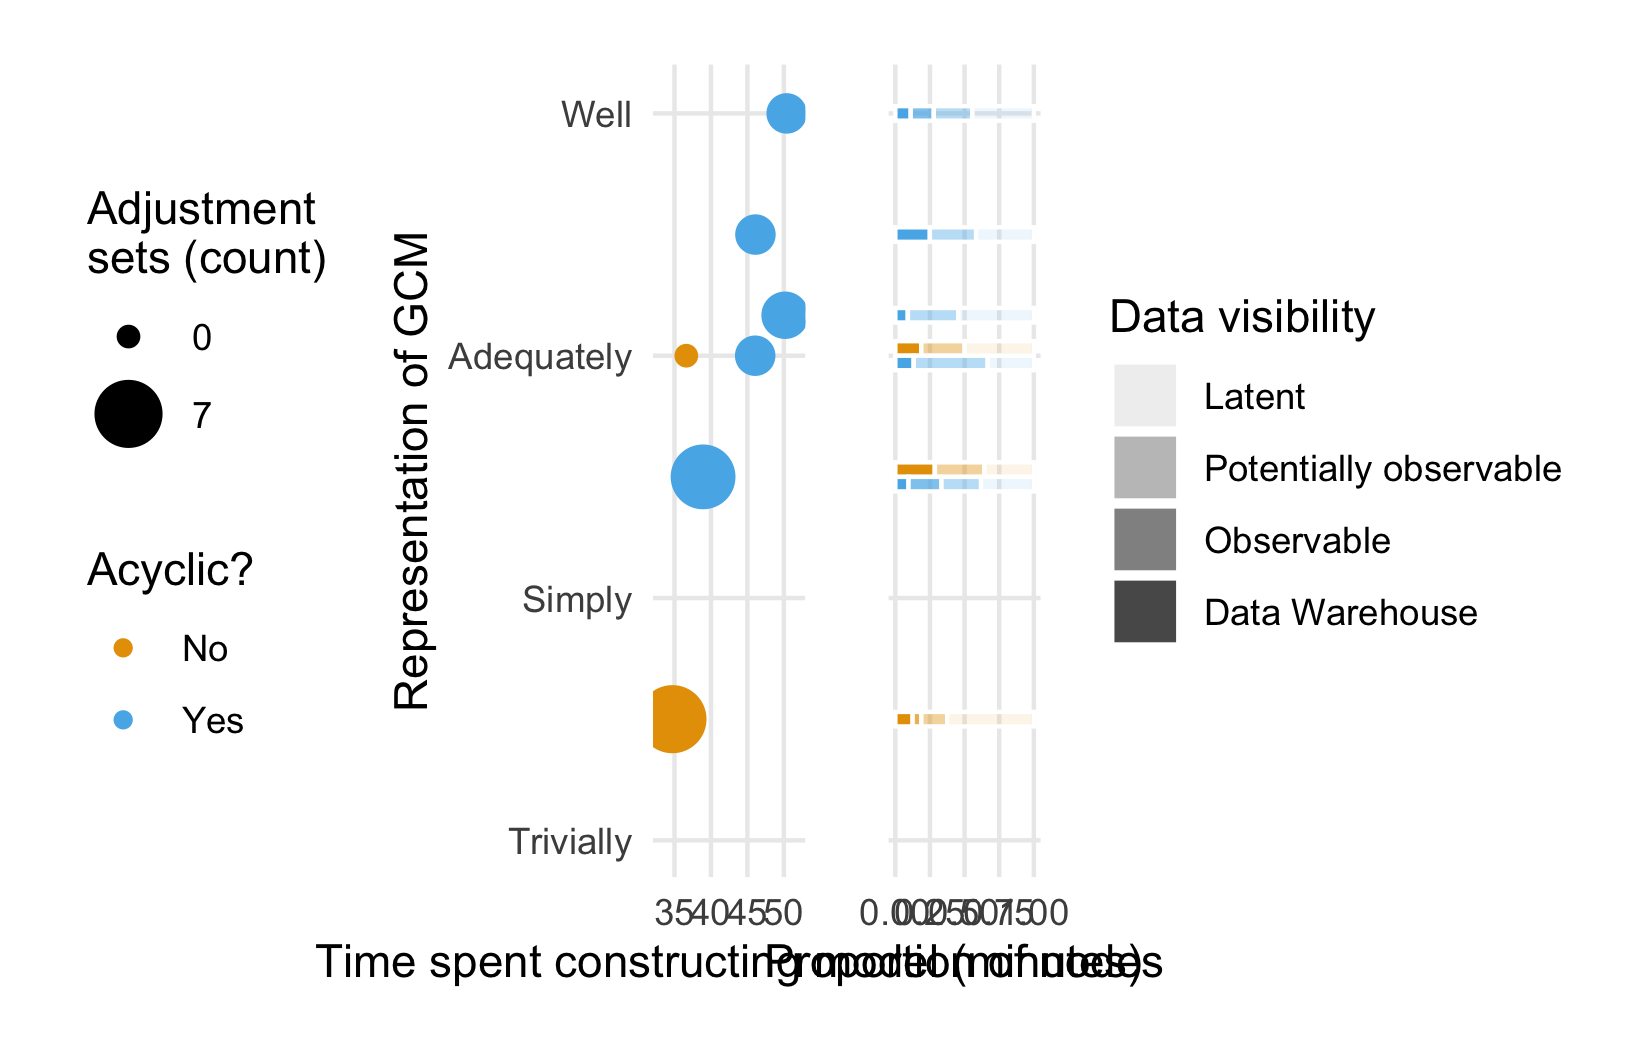
\includegraphics[keepaspectratio]{elicited-DAG-analysis_files/figure-pdf/unnamed-chunk-19-1.png}}

\begin{Shaded}
\begin{Highlighting}[]
\FunctionTok{ggsave}\NormalTok{(}\StringTok{"figures/FIG{-}{-}time{-}modelling{-}and{-}representation.jpg"}\NormalTok{, }
       \AttributeTok{plot =}\NormalTok{ p\_time\_and\_representation\_1,}
       \AttributeTok{width =} \DecValTok{10}\NormalTok{, }\AttributeTok{height =} \DecValTok{5}\NormalTok{, }
       \AttributeTok{dpi =} \DecValTok{300}\NormalTok{)}

\FunctionTok{ggsave}\NormalTok{(}\StringTok{"figures/FIG{-}{-}time{-}modelling{-}and{-}representation.svg"}\NormalTok{, }
       \AttributeTok{plot =}\NormalTok{ p\_time\_and\_representation\_1,}
       \AttributeTok{width =} \DecValTok{25}\NormalTok{, }\AttributeTok{height =} \DecValTok{10}\NormalTok{, }\AttributeTok{units =} \StringTok{"cm"}\NormalTok{)}
\end{Highlighting}
\end{Shaded}

This version displays all in one (is a little dense)

\begin{Shaded}
\begin{Highlighting}[]
\CommentTok{\# denser option {-} radial arc bars for observable}
\FunctionTok{library}\NormalTok{(scales)}
\FunctionTok{library}\NormalTok{(ggforce)}
\FunctionTok{library}\NormalTok{(patchwork)}
\FunctionTok{library}\NormalTok{(cowplot)}

\NormalTok{hue1 }\OtherTok{\textless{}{-}} \FunctionTok{palette.colors}\NormalTok{(}\DecValTok{3}\NormalTok{, }\AttributeTok{palette =} \StringTok{"Okabe{-}Ito"}\NormalTok{)[[}\DecValTok{2}\NormalTok{]]}
\NormalTok{hue2 }\OtherTok{\textless{}{-}} \FunctionTok{palette.colors}\NormalTok{(}\DecValTok{3}\NormalTok{, }\AttributeTok{palette =} \StringTok{"Okabe{-}Ito"}\NormalTok{)[[}\DecValTok{3}\NormalTok{]]}

\CommentTok{\# Main plot {-} hide all legends}
\NormalTok{p\_main }\OtherTok{\textless{}{-}}\NormalTok{ gcm\_metrics }\SpecialCharTok{|\textgreater{}} 
    \FunctionTok{mutate}\NormalTok{(}
        \AttributeTok{x\_duration =} \FunctionTok{as.numeric}\NormalTok{(Modelling.duration, }\AttributeTok{units =} \StringTok{"minutes"}\NormalTok{),}
        \AttributeTok{y\_validity =}\NormalTok{ GCM.validity }\SpecialCharTok{*} \DecValTok{10} \SpecialCharTok{+} \DecValTok{20}
\NormalTok{    ) }\SpecialCharTok{|\textgreater{}} 
    \FunctionTok{mutate}\NormalTok{(}\AttributeTok{acyclic =} \FunctionTok{if\_else}\NormalTok{(acyclic, }\StringTok{"Yes, DAG"}\NormalTok{, }\StringTok{"No, contained cycles"}\NormalTok{)) }\SpecialCharTok{|\textgreater{}} 
    \FunctionTok{ggplot}\NormalTok{(}\FunctionTok{aes}\NormalTok{(}
        \AttributeTok{color =}\NormalTok{ acyclic,}
        \AttributeTok{size =}\NormalTok{ n\_adj\_sets}
\NormalTok{    )) }\SpecialCharTok{+}
    \FunctionTok{geom\_arc\_bar}\NormalTok{(}\FunctionTok{aes}\NormalTok{(}
        \AttributeTok{x0 =}\NormalTok{ x\_duration,}
        \AttributeTok{y0 =}\NormalTok{ y\_validity,}
        \AttributeTok{r0 =} \DecValTok{0}\NormalTok{,}
        \AttributeTok{r =} \FloatTok{1.1}\NormalTok{,}
        \AttributeTok{start =}\NormalTok{ pi }\SpecialCharTok{+} \DecValTok{2} \SpecialCharTok{*}\NormalTok{ (p\_dw }\SpecialCharTok{+}\NormalTok{ p\_o }\SpecialCharTok{+}\NormalTok{ p\_po) }\SpecialCharTok{*}\NormalTok{ pi,}
        \AttributeTok{end =} \DecValTok{3} \SpecialCharTok{*}\NormalTok{ pi}
\NormalTok{    ),}
        \AttributeTok{fill =} \StringTok{"white"}\NormalTok{,}
        \AttributeTok{linewidth =} \DecValTok{0}\NormalTok{,}
    \AttributeTok{alpha =} \FloatTok{0.8}\NormalTok{, }\AttributeTok{show.legend =} \ConstantTok{FALSE}\NormalTok{) }\SpecialCharTok{+}
    \FunctionTok{geom\_arc\_bar}\NormalTok{(}\FunctionTok{aes}\NormalTok{(}
        \AttributeTok{x0 =}\NormalTok{ x\_duration, }
        \AttributeTok{y0 =}\NormalTok{ y\_validity,}
        \AttributeTok{fill =}\NormalTok{ acyclic,}
        \AttributeTok{size =} \DecValTok{1}\NormalTok{,}
        \AttributeTok{r0 =} \DecValTok{0}\NormalTok{,}
        \AttributeTok{r =} \FloatTok{1.5}\NormalTok{,}
        \AttributeTok{start =}\NormalTok{ pi, }
        \AttributeTok{end =}\NormalTok{ pi }\SpecialCharTok{+} \DecValTok{2} \SpecialCharTok{*}\NormalTok{ p\_dw }\SpecialCharTok{*}\NormalTok{ pi}
\NormalTok{    ), }
        \AttributeTok{linewidth =} \DecValTok{0}\NormalTok{,}
    \AttributeTok{alpha =} \DecValTok{1}\NormalTok{, }\AttributeTok{show.legend =} \ConstantTok{FALSE}\NormalTok{) }\SpecialCharTok{+} 
    \FunctionTok{geom\_arc\_bar}\NormalTok{(}\FunctionTok{aes}\NormalTok{(}
        \AttributeTok{x0 =}\NormalTok{ x\_duration, }
        \AttributeTok{y0 =}\NormalTok{ y\_validity,}
        \AttributeTok{fill =}\NormalTok{ acyclic,}
        \AttributeTok{r0 =} \DecValTok{0}\NormalTok{,}
        \AttributeTok{r =} \FloatTok{1.3}\NormalTok{,}
        \AttributeTok{start =}\NormalTok{ pi }\SpecialCharTok{+} \DecValTok{2} \SpecialCharTok{*}\NormalTok{ p\_dw }\SpecialCharTok{*}\NormalTok{ pi, }
        \AttributeTok{end =}\NormalTok{ pi }\SpecialCharTok{+} \DecValTok{2} \SpecialCharTok{*}\NormalTok{ (p\_dw }\SpecialCharTok{+}\NormalTok{ p\_o) }\SpecialCharTok{*}\NormalTok{ pi}
\NormalTok{    ), }
        \AttributeTok{linewidth =} \DecValTok{0}\NormalTok{,}
    \AttributeTok{alpha =} \FloatTok{0.6}\NormalTok{, }\AttributeTok{show.legend =} \ConstantTok{FALSE}\NormalTok{) }\SpecialCharTok{+} 
    \FunctionTok{geom\_arc\_bar}\NormalTok{(}\FunctionTok{aes}\NormalTok{(}
        \AttributeTok{x0 =}\NormalTok{ x\_duration, }
        \AttributeTok{y0 =}\NormalTok{ y\_validity,}
        \AttributeTok{fill =}\NormalTok{ acyclic,}
        \AttributeTok{r0 =} \DecValTok{0}\NormalTok{,}
        \AttributeTok{r =} \FloatTok{1.1}\NormalTok{,}
        \AttributeTok{start =}\NormalTok{ pi }\SpecialCharTok{+} \DecValTok{2} \SpecialCharTok{*}\NormalTok{ (p\_dw }\SpecialCharTok{+}\NormalTok{ p\_o) }\SpecialCharTok{*}\NormalTok{ pi, }
        \AttributeTok{end =}\NormalTok{ pi }\SpecialCharTok{+} \DecValTok{2} \SpecialCharTok{*}\NormalTok{ (p\_dw }\SpecialCharTok{+}\NormalTok{ p\_o }\SpecialCharTok{+}\NormalTok{ p\_po) }\SpecialCharTok{*}\NormalTok{ pi}
\NormalTok{    ), }
        \AttributeTok{linewidth =} \DecValTok{0}\NormalTok{,}
    \AttributeTok{alpha =} \FloatTok{0.4}\NormalTok{, }\AttributeTok{show.legend =} \ConstantTok{FALSE}\NormalTok{) }\SpecialCharTok{+} 
    \FunctionTok{geom\_point}\NormalTok{(}\FunctionTok{aes}\NormalTok{(}
        \AttributeTok{x =}\NormalTok{ x\_duration,}
        \AttributeTok{y =}\NormalTok{ y\_validity)) }\SpecialCharTok{+}
    \FunctionTok{scale\_y\_continuous}\NormalTok{(}
        \AttributeTok{limits =} \FunctionTok{c}\NormalTok{(}\DecValTok{30}\NormalTok{, }\DecValTok{61}\NormalTok{),}
        \AttributeTok{breaks =} \FunctionTok{c}\NormalTok{(}\DecValTok{30}\NormalTok{, }\DecValTok{40}\NormalTok{, }\DecValTok{50}\NormalTok{, }\DecValTok{60}\NormalTok{),}
        \AttributeTok{labels =} \FunctionTok{c}\NormalTok{(}\StringTok{"Trivially"}\NormalTok{, }\StringTok{"Simply"}\NormalTok{, }\StringTok{"Adequately"}\NormalTok{, }\StringTok{"Well"}\NormalTok{),}
        \AttributeTok{name =} \StringTok{"Representation of GCM"}\NormalTok{) }\SpecialCharTok{+}
    \FunctionTok{scale\_x\_continuous}\NormalTok{(}
        \AttributeTok{limits =} \FunctionTok{c}\NormalTok{(}\DecValTok{30}\NormalTok{, }\DecValTok{55}\NormalTok{),  }\CommentTok{\# was 55 to  Keep original limits for the data}
        \AttributeTok{breaks =} \FunctionTok{c}\NormalTok{(}\DecValTok{30}\NormalTok{, }\DecValTok{40}\NormalTok{, }\DecValTok{50}\NormalTok{),}
        \AttributeTok{name =} \StringTok{"Time spent constructing model (minutes)"}\NormalTok{) }\SpecialCharTok{+}
    \FunctionTok{scale\_size}\NormalTok{(}\AttributeTok{range =} \FunctionTok{c}\NormalTok{(}\DecValTok{2}\NormalTok{, }\DecValTok{7}\NormalTok{),}
               \AttributeTok{breaks =} \FunctionTok{range}\NormalTok{(gcm\_metrics}\SpecialCharTok{$}\NormalTok{n\_adj\_sets),}
               \AttributeTok{name =} \StringTok{"Adjustment}\SpecialCharTok{\textbackslash{}n}\StringTok{sets"}\NormalTok{) }\SpecialCharTok{+}
    \FunctionTok{scale\_color\_manual}\NormalTok{(}\AttributeTok{values =} \FunctionTok{c}\NormalTok{(hue1, hue2), }\AttributeTok{name =} \StringTok{"Is DAG?"}\NormalTok{) }\SpecialCharTok{+}
    \FunctionTok{scale\_fill\_manual}\NormalTok{(}\AttributeTok{values =} \FunctionTok{c}\NormalTok{(hue1, hue2), }\AttributeTok{guide =} \StringTok{"none"}\NormalTok{) }\SpecialCharTok{+}
    \FunctionTok{theme\_minimal}\NormalTok{() }\SpecialCharTok{+}
    \FunctionTok{coord\_fixed}\NormalTok{(}\AttributeTok{ratio =} \DecValTok{1}\NormalTok{, }\AttributeTok{clip =} \StringTok{"off"}\NormalTok{) }\SpecialCharTok{+}
    \FunctionTok{theme}\NormalTok{(}
        \AttributeTok{legend.position =} \StringTok{"none"}\NormalTok{,  }\CommentTok{\# Hide legends from main plot}
        \CommentTok{\# panel.grid.major.x = element\_blank(),  \# Remove vertical gridlines}
        \AttributeTok{panel.grid.minor =} \FunctionTok{element\_blank}\NormalTok{(),}
        \AttributeTok{plot.margin =} \FunctionTok{margin}\NormalTok{(}\DecValTok{10}\NormalTok{, }\DecValTok{10}\NormalTok{, }\DecValTok{10}\NormalTok{, }\DecValTok{10}\NormalTok{)}
\NormalTok{    )}
\end{Highlighting}
\end{Shaded}

\begin{verbatim}
Warning: Using `size` aesthetic for lines was deprecated in ggplot2 3.4.0.
i Please use `linewidth` instead.
\end{verbatim}

\begin{Shaded}
\begin{Highlighting}[]
\CommentTok{\# Create a dummy plot just to extract the legends}
\NormalTok{p\_for\_legend }\OtherTok{\textless{}{-}}\NormalTok{ gcm\_metrics }\SpecialCharTok{|\textgreater{}} 
    \FunctionTok{mutate}\NormalTok{(}
        \AttributeTok{x\_duration =} \FunctionTok{as.numeric}\NormalTok{(Modelling.duration, }\AttributeTok{units =} \StringTok{"minutes"}\NormalTok{),}
        \AttributeTok{y\_validity =}\NormalTok{ GCM.validity }\SpecialCharTok{*} \DecValTok{10} \SpecialCharTok{+} \DecValTok{20}
\NormalTok{    ) }\SpecialCharTok{|\textgreater{}} 
    \FunctionTok{mutate}\NormalTok{(}\AttributeTok{acyclic =} \FunctionTok{if\_else}\NormalTok{(acyclic, }\StringTok{"Yes, DAG"}\NormalTok{, }\StringTok{"No, contained cycles"}\NormalTok{)) }\SpecialCharTok{|\textgreater{}} 
    \FunctionTok{ggplot}\NormalTok{(}\FunctionTok{aes}\NormalTok{(}
        \AttributeTok{x =}\NormalTok{ x\_duration,}
        \AttributeTok{y =}\NormalTok{ y\_validity,}
        \AttributeTok{color =}\NormalTok{ acyclic,}
        \AttributeTok{size =}\NormalTok{ n\_adj\_sets}
\NormalTok{    )) }\SpecialCharTok{+}
    \FunctionTok{geom\_point}\NormalTok{() }\SpecialCharTok{+}
    \FunctionTok{scale\_size}\NormalTok{(}\AttributeTok{range =} \FunctionTok{c}\NormalTok{(}\DecValTok{2}\NormalTok{, }\DecValTok{7}\NormalTok{),}
               \AttributeTok{breaks =} \FunctionTok{range}\NormalTok{(gcm\_metrics}\SpecialCharTok{$}\NormalTok{n\_adj\_sets),}
               \AttributeTok{name =} \StringTok{"N adjustment sets"}\NormalTok{) }\SpecialCharTok{+}
    \FunctionTok{scale\_color\_manual}\NormalTok{(}\AttributeTok{values =} \FunctionTok{c}\NormalTok{(hue1, hue2), }\AttributeTok{name =} \StringTok{"Is DAG?"}\NormalTok{) }\SpecialCharTok{+}
    \FunctionTok{theme\_minimal}\NormalTok{() }\SpecialCharTok{+}
    \FunctionTok{theme}\NormalTok{(}\AttributeTok{legend.box =} \StringTok{"vertical"}\NormalTok{)}

\CommentTok{\# Extract the legend}
\NormalTok{legend\_extracted }\OtherTok{\textless{}{-}}\NormalTok{ cowplot}\SpecialCharTok{::}\FunctionTok{get\_legend}\NormalTok{(p\_for\_legend)}

\CommentTok{\# Custom legend plot showing the arc explanation}
\NormalTok{p\_legend\_arcs }\OtherTok{\textless{}{-}} \FunctionTok{ggplot}\NormalTok{() }\SpecialCharTok{+}
    \FunctionTok{geom\_arc\_bar}\NormalTok{(}\FunctionTok{aes}\NormalTok{(}\AttributeTok{x0 =} \DecValTok{0}\NormalTok{, }\AttributeTok{y0 =} \DecValTok{0}\NormalTok{, }\AttributeTok{r0 =} \FloatTok{0.1}\NormalTok{, }\AttributeTok{r =} \FloatTok{0.8}\NormalTok{, }\AttributeTok{start =}\NormalTok{ pi, }\AttributeTok{end =}\NormalTok{ pi }\SpecialCharTok{+}\NormalTok{ pi}\SpecialCharTok{/}\DecValTok{3}\NormalTok{),}
             \AttributeTok{fill =} \StringTok{"black"}\NormalTok{, }\AttributeTok{alpha =} \DecValTok{1}\NormalTok{, }\AttributeTok{linewidth =} \DecValTok{0}\NormalTok{) }\SpecialCharTok{+}
    \FunctionTok{geom\_arc\_bar}\NormalTok{(}\FunctionTok{aes}\NormalTok{(}\AttributeTok{x0 =} \DecValTok{0}\NormalTok{, }\AttributeTok{y0 =} \DecValTok{0}\NormalTok{, }\AttributeTok{r0 =} \FloatTok{0.1}\NormalTok{, }\AttributeTok{r =} \FloatTok{0.6}\NormalTok{, }\AttributeTok{start =}\NormalTok{ pi }\SpecialCharTok{+}\NormalTok{ pi}\SpecialCharTok{/}\DecValTok{3}\NormalTok{, }\AttributeTok{end =}\NormalTok{ pi }\SpecialCharTok{+}\NormalTok{ (}\DecValTok{2}\SpecialCharTok{*}\NormalTok{pi}\SpecialCharTok{/}\DecValTok{3}\NormalTok{)),}
             \AttributeTok{fill =} \StringTok{"black"}\NormalTok{, }\AttributeTok{alpha =} \FloatTok{0.6}\NormalTok{, }\AttributeTok{linewidth =} \DecValTok{0}\NormalTok{) }\SpecialCharTok{+}
    \FunctionTok{geom\_arc\_bar}\NormalTok{(}\FunctionTok{aes}\NormalTok{(}\AttributeTok{x0 =} \DecValTok{0}\NormalTok{, }\AttributeTok{y0 =} \DecValTok{0}\NormalTok{, }\AttributeTok{r0 =} \FloatTok{0.1}\NormalTok{, }\AttributeTok{r =} \FloatTok{0.4}\NormalTok{, }\AttributeTok{start =}\NormalTok{ pi }\SpecialCharTok{+}\NormalTok{ (}\DecValTok{2}\SpecialCharTok{*}\NormalTok{pi}\SpecialCharTok{/}\DecValTok{3}\NormalTok{), }\AttributeTok{end =} \DecValTok{2} \SpecialCharTok{*}\NormalTok{ pi),}
             \AttributeTok{fill =} \StringTok{"black"}\NormalTok{, }\AttributeTok{alpha =} \FloatTok{0.4}\NormalTok{, }\AttributeTok{linewidth =} \DecValTok{0}\NormalTok{) }\SpecialCharTok{+}
    \FunctionTok{annotate}\NormalTok{(}\StringTok{"text"}\NormalTok{, }
             \AttributeTok{x =} \FloatTok{0.5}\NormalTok{, }\AttributeTok{y =} \SpecialCharTok{{-}}\FloatTok{0.9}\NormalTok{,}
             \AttributeTok{label =} \StringTok{"In data}\SpecialCharTok{\textbackslash{}n}\StringTok{warehouse"}\NormalTok{, }
             \AttributeTok{hjust =} \DecValTok{0}\NormalTok{, }\AttributeTok{size =} \DecValTok{3}\NormalTok{, }\AttributeTok{color =} \StringTok{"black"}\NormalTok{) }\SpecialCharTok{+}
    \FunctionTok{annotate}\NormalTok{(}\StringTok{"text"}\NormalTok{, }
             \AttributeTok{x =} \FloatTok{0.5}\NormalTok{, }\AttributeTok{y =} \DecValTok{0}\NormalTok{, }
             \AttributeTok{label =} \StringTok{"Observable"}\NormalTok{, }
             \AttributeTok{hjust =} \DecValTok{0}\NormalTok{, }\AttributeTok{size =} \DecValTok{3}\NormalTok{, }\AttributeTok{color =} \FunctionTok{adjustcolor}\NormalTok{(}\StringTok{"black"}\NormalTok{, }\AttributeTok{alpha.f =} \FloatTok{0.8}\NormalTok{)) }\SpecialCharTok{+}
    \FunctionTok{annotate}\NormalTok{(}\StringTok{"text"}\NormalTok{, }\AttributeTok{x =} \FloatTok{0.5}\NormalTok{, }\AttributeTok{y =} \FloatTok{0.9}\NormalTok{, }\AttributeTok{label =} \StringTok{"Potentially}\SpecialCharTok{\textbackslash{}n}\StringTok{observable"}\NormalTok{, }
             \AttributeTok{hjust =} \DecValTok{0}\NormalTok{, }\AttributeTok{size =} \DecValTok{3}\NormalTok{, }\AttributeTok{color =} \FunctionTok{adjustcolor}\NormalTok{(}\StringTok{"black"}\NormalTok{, }\AttributeTok{alpha.f =} \FloatTok{0.6}\NormalTok{)) }\SpecialCharTok{+}
    \FunctionTok{annotate}\NormalTok{(}\StringTok{"segment"}\NormalTok{, }\AttributeTok{x =} \FloatTok{0.1}\NormalTok{, }\AttributeTok{xend =} \FloatTok{0.4}\NormalTok{, }\AttributeTok{y =} \SpecialCharTok{{-}}\FloatTok{0.5}\NormalTok{, }\AttributeTok{yend =} \SpecialCharTok{{-}}\FloatTok{0.6}\NormalTok{, }\AttributeTok{color =} \StringTok{"black"}\NormalTok{) }\SpecialCharTok{+}
    \FunctionTok{annotate}\NormalTok{(}\StringTok{"segment"}\NormalTok{, }\AttributeTok{x =} \DecValTok{0}\NormalTok{, }\AttributeTok{xend =} \FloatTok{0.4}\NormalTok{, }\AttributeTok{y =} \DecValTok{0}\NormalTok{, }\AttributeTok{yend =} \DecValTok{0}\NormalTok{, }
             \AttributeTok{color =} \StringTok{"black"}\NormalTok{, }\AttributeTok{alpha =} \FloatTok{0.6}\NormalTok{) }\SpecialCharTok{+}
    \FunctionTok{annotate}\NormalTok{(}\StringTok{"segment"}\NormalTok{, }\AttributeTok{x =} \FloatTok{0.1}\NormalTok{, }\AttributeTok{xend =} \FloatTok{0.4}\NormalTok{, }\AttributeTok{y =} \FloatTok{0.4}\NormalTok{, }\AttributeTok{yend =} \FloatTok{0.6}\NormalTok{, }
             \AttributeTok{color =} \StringTok{"black"}\NormalTok{, }\AttributeTok{alpha =} \FloatTok{0.4}\NormalTok{) }\SpecialCharTok{+}
    \FunctionTok{coord\_fixed}\NormalTok{() }\SpecialCharTok{+}
    \FunctionTok{xlim}\NormalTok{(}\SpecialCharTok{{-}}\DecValTok{1}\NormalTok{, }\FloatTok{2.5}\NormalTok{) }\SpecialCharTok{+}
    \FunctionTok{ylim}\NormalTok{(}\SpecialCharTok{{-}}\FloatTok{1.3}\NormalTok{, }\FloatTok{1.3}\NormalTok{) }\SpecialCharTok{+}
    \FunctionTok{labs}\NormalTok{(}\AttributeTok{title =} \StringTok{"Proportion of nodes:"}\NormalTok{) }\SpecialCharTok{+}
    \FunctionTok{theme\_void}\NormalTok{() }\SpecialCharTok{+}
    \FunctionTok{theme}\NormalTok{(}\AttributeTok{plot.title =} \FunctionTok{element\_text}\NormalTok{(}\AttributeTok{size =} \DecValTok{9}\NormalTok{, }\AttributeTok{face =} \StringTok{"bold"}\NormalTok{))}

\CommentTok{\# Combine the arc legend and extracted legends vertically}
\NormalTok{legend\_column }\OtherTok{\textless{}{-}}\NormalTok{ cowplot}\SpecialCharTok{::}\FunctionTok{plot\_grid}\NormalTok{(}
\NormalTok{    legend\_extracted,}
\NormalTok{    p\_legend\_arcs,}
    \AttributeTok{ncol =} \DecValTok{2}\NormalTok{,}
    \AttributeTok{rel\_heights =} \FunctionTok{c}\NormalTok{(}\DecValTok{1}\NormalTok{, }\DecValTok{1}\NormalTok{)}
\NormalTok{)}

\CommentTok{\# Combine main plot with legend column}
\NormalTok{p\_time\_and\_representation }\OtherTok{\textless{}{-}}\NormalTok{ cowplot}\SpecialCharTok{::}\FunctionTok{plot\_grid}\NormalTok{(}
\NormalTok{    p\_main,}
\NormalTok{    legend\_column,}
    \AttributeTok{ncol =} \DecValTok{2}\NormalTok{,}
    \AttributeTok{rel\_widths =} \FunctionTok{c}\NormalTok{(}\DecValTok{1}\NormalTok{, }\DecValTok{1}\NormalTok{)  }\CommentTok{\# Adjust ratio as needed}
\NormalTok{)}

\NormalTok{p\_time\_and\_representation}
\end{Highlighting}
\end{Shaded}

\pandocbounded{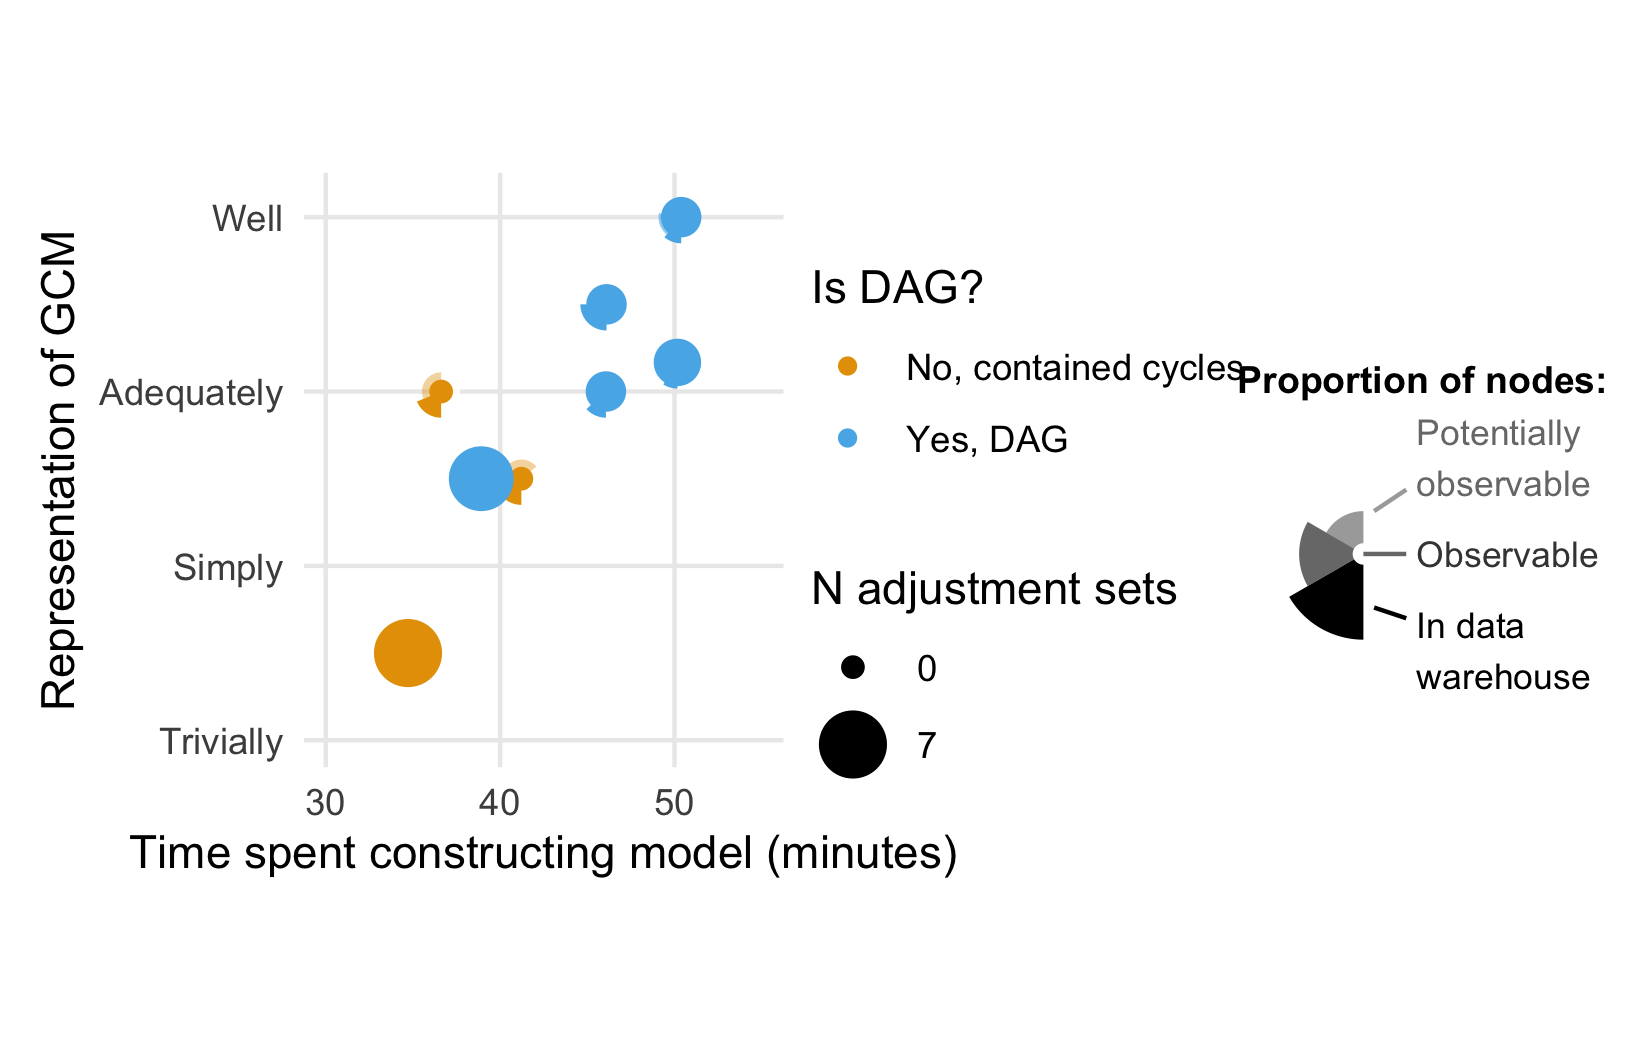
\includegraphics[keepaspectratio]{elicited-DAG-analysis_files/figure-pdf/unnamed-chunk-20-1.png}}

\begin{Shaded}
\begin{Highlighting}[]
\FunctionTok{ggsave}\NormalTok{(}\StringTok{"figures/FIG{-}{-}time{-}modelling{-}and{-}representation{-}arc{-}bars.jpg"}\NormalTok{, }
       \AttributeTok{plot =}\NormalTok{ p\_time\_and\_representation,}
       \AttributeTok{width =} \DecValTok{10}\NormalTok{, }\AttributeTok{height =} \DecValTok{5}\NormalTok{, }
       \AttributeTok{dpi =} \DecValTok{900}\NormalTok{)}
\end{Highlighting}
\end{Shaded}

As a table:

\begin{Shaded}
\begin{Highlighting}[]
\NormalTok{gcm\_metrics }\SpecialCharTok{|\textgreater{}} 
    \FunctionTok{mutate}\NormalTok{(}\AttributeTok{acyclic =} \FunctionTok{if\_else}\NormalTok{(acyclic, }\StringTok{"Yes, DAG"}\NormalTok{, }\StringTok{"No, contained cycles"}\NormalTok{)) }\SpecialCharTok{|\textgreater{}} 
    \FunctionTok{arrange}\NormalTok{(}\FunctionTok{desc}\NormalTok{(Modelling.duration)) }\SpecialCharTok{|\textgreater{}} 
    \FunctionTok{select}\NormalTok{(Modelling.duration, GCM.validity, acyclic, n\_adj\_sets, p\_dw, p\_o, p\_po, p\_l)}
\end{Highlighting}
\end{Shaded}

\begin{verbatim}
# A tibble: 8 x 8
  Modelling.duration GCM.validity acyclic   n_adj_sets   p_dw    p_o  p_po   p_l
  <Period>                  <dbl> <chr>          <int>  <dbl>  <dbl> <dbl> <dbl>
1 50M 23S                    4    Yes, DAG           1 0.111  0.167  0.278 0.444
2 50M 10S                    3.17 Yes, DAG           2 0.0909 0      0.364 0.545
3 46M 6S                     3.5  Yes, DAG           1 0.25   0      0.333 0.417
4 46M 4S                     3    Yes, DAG           1 0.133  0      0.533 0.333
5 41M 13S                    2.5  No, cont~          0 0.286  0      0.357 0.357
6 38M 55S                    2.5  Yes, DAG           6 0.0952 0.238  0.286 0.381
7 36M 37S                    3    No, cont~          0 0.188  0      0.312 0.5  
8 34M 43S                    1.5  No, cont~          7 0.125  0.0625 0.188 0.625
\end{verbatim}

\paragraph{Figure (OPTIONAL): Time spent with model and modelling
utility - including graph
similarity}\label{figure-optional-time-spent-with-model-and-modelling-utility---including-graph-similarity}

Graph similarity computed with d-Measure.

Only showing the upper 50\% of edges

\begin{Shaded}
\begin{Highlighting}[]
\NormalTok{d\_between\_models\_median }\OtherTok{\textless{}{-}} \FunctionTok{median}\NormalTok{(}\FunctionTok{pull}\NormalTok{(d\_edges, edge\_d))}

\FunctionTok{print}\NormalTok{(}\FunctionTok{str\_c}\NormalTok{(}\StringTok{"Median d{-}measure between models is "}\NormalTok{, }\FunctionTok{round}\NormalTok{(d\_between\_models\_median, }\DecValTok{3}\NormalTok{)))}
\end{Highlighting}
\end{Shaded}

\begin{verbatim}
[1] "Median d-measure between models is 0.281"
\end{verbatim}

\begin{Shaded}
\begin{Highlighting}[]
\NormalTok{d\_edges }\SpecialCharTok{|\textgreater{}} 
    \FunctionTok{slice}\NormalTok{(}\DecValTok{1}\NormalTok{)}
\end{Highlighting}
\end{Shaded}

\begin{verbatim}
# A tibble: 1 x 4
  from  to    edge_d edge_w
  <fct> <fct>  <dbl>  <dbl>
1 S3    S4     0.172   5.82
\end{verbatim}

\begin{Shaded}
\begin{Highlighting}[]
\NormalTok{d\_edges }\SpecialCharTok{|\textgreater{}} 
    \FunctionTok{arrange}\NormalTok{(edge\_w) }\SpecialCharTok{|\textgreater{}} 
    \FunctionTok{slice}\NormalTok{(}\DecValTok{1}\NormalTok{)}
\end{Highlighting}
\end{Shaded}

\begin{verbatim}
# A tibble: 1 x 4
  from  to    edge_d edge_w
  <fct> <fct>  <dbl>  <dbl>
1 S2    S5     0.475   2.10
\end{verbatim}

\begin{Shaded}
\begin{Highlighting}[]
\NormalTok{d\_between\_models\_by\_time\_and\_utility }\OtherTok{\textless{}{-}} 
\NormalTok{    d\_edges }\SpecialCharTok{|\textgreater{}} 
    \FunctionTok{inner\_join}\NormalTok{(}
\NormalTok{        gcm\_metrics }\SpecialCharTok{|\textgreater{}} 
            \FunctionTok{mutate}\NormalTok{(}\AttributeTok{from =}\NormalTok{ Model) }\SpecialCharTok{|\textgreater{}} 
            \FunctionTok{select}\NormalTok{(from, }\AttributeTok{xfrom =}\NormalTok{ Modelling.duration, }\AttributeTok{yfrom =}\NormalTok{ GCM.validity)}
\NormalTok{    ) }\SpecialCharTok{|\textgreater{}} 
    \FunctionTok{inner\_join}\NormalTok{(}
\NormalTok{        gcm\_metrics }\SpecialCharTok{|\textgreater{}} 
            \FunctionTok{mutate}\NormalTok{(}\AttributeTok{to =}\NormalTok{ Model) }\SpecialCharTok{|\textgreater{}} 
            \FunctionTok{select}\NormalTok{(to, }\AttributeTok{xto =}\NormalTok{ Modelling.duration, }\AttributeTok{yto =}\NormalTok{ GCM.validity)}
\NormalTok{    ) }
\end{Highlighting}
\end{Shaded}

\begin{verbatim}
Joining with `by = join_by(from)`
Joining with `by = join_by(to)`
\end{verbatim}

\begin{Shaded}
\begin{Highlighting}[]
\NormalTok{p\_time\_and\_representaion\_with\_distance }\OtherTok{\textless{}{-}} 
\NormalTok{    gcm\_metrics }\SpecialCharTok{|\textgreater{}} 
    \FunctionTok{mutate}\NormalTok{(}\AttributeTok{acyclic =} \FunctionTok{if\_else}\NormalTok{(acyclic, }\StringTok{"Yes, DAG"}\NormalTok{, }\StringTok{"No, contained cycles"}\NormalTok{)) }\SpecialCharTok{|\textgreater{}} 
    \FunctionTok{ggplot}\NormalTok{() }\SpecialCharTok{+}
    \FunctionTok{geom\_segment}\NormalTok{(}
        \AttributeTok{data =}\NormalTok{ d\_between\_models\_by\_time\_and\_utility }\SpecialCharTok{|\textgreater{}} 
            \FunctionTok{filter}\NormalTok{(edge\_d }\SpecialCharTok{\textless{}}\NormalTok{ d\_between\_models\_median),}
        \FunctionTok{aes}\NormalTok{(}\AttributeTok{x =}\NormalTok{ xfrom, }\AttributeTok{xend =}\NormalTok{ xto, }\AttributeTok{y =}\NormalTok{ yfrom, }\AttributeTok{yend =}\NormalTok{ yto,}
            \AttributeTok{alpha =}\NormalTok{ edge\_w), }\AttributeTok{size =} \FloatTok{0.5}\NormalTok{, }\AttributeTok{color =} \StringTok{"black"}\NormalTok{) }\SpecialCharTok{+}
    \FunctionTok{geom\_point}\NormalTok{(}\AttributeTok{data =}\NormalTok{ gcm\_metrics, }
               \FunctionTok{aes}\NormalTok{(}\AttributeTok{x =}\NormalTok{ Modelling.duration, }\AttributeTok{y =}\NormalTok{ GCM.validity, }\AttributeTok{size =}\NormalTok{ n\_adj\_sets, }\AttributeTok{colour =}\NormalTok{ acyclic)) }\SpecialCharTok{+}
    \CommentTok{\# geom\_text(aes(label = Model), nudge\_y = {-}.1) +}
    \FunctionTok{scale\_y\_continuous}\NormalTok{(}\AttributeTok{limits =} \FunctionTok{c}\NormalTok{(}\DecValTok{1}\NormalTok{, }\DecValTok{4}\NormalTok{),}
                       \AttributeTok{breaks =} \FunctionTok{c}\NormalTok{(}\DecValTok{1}\SpecialCharTok{:}\DecValTok{4}\NormalTok{),}
                       \AttributeTok{labels =} \FunctionTok{c}\NormalTok{(}\StringTok{"Trivially"}\NormalTok{, }\StringTok{"Simply"}\NormalTok{, }\StringTok{"Adequately"}\NormalTok{, }\StringTok{"Well"}\NormalTok{),}
                       \AttributeTok{name =} \StringTok{"Representation of GCM"}\NormalTok{) }\SpecialCharTok{+}
     \FunctionTok{scale\_x\_time}\NormalTok{(}\AttributeTok{labels =} \FunctionTok{label\_time}\NormalTok{(}\AttributeTok{format =} \StringTok{"\%M:\%S"}\NormalTok{),}
                  \AttributeTok{name =} \StringTok{"Time spent constructing model (minutes)"}\NormalTok{) }\SpecialCharTok{+}
    \FunctionTok{scale\_size}\NormalTok{(}\AttributeTok{range =} \FunctionTok{c}\NormalTok{(}\DecValTok{2}\NormalTok{,}\DecValTok{7}\NormalTok{),}
               \AttributeTok{breaks =} \FunctionTok{range}\NormalTok{(gcm\_metrics}\SpecialCharTok{$}\NormalTok{n\_adj\_sets),}
               \CommentTok{\# labels = c("None", )}
               \AttributeTok{name =} \StringTok{"N adjustment sets"}\NormalTok{) }\SpecialCharTok{+}
    \FunctionTok{scale\_alpha\_continuous}\NormalTok{(}\AttributeTok{range =} \FunctionTok{c}\NormalTok{(}\FloatTok{0.1}\NormalTok{, }\FloatTok{0.7}\NormalTok{), }\AttributeTok{guide =} \StringTok{"none"}\NormalTok{) }\SpecialCharTok{+}
    \FunctionTok{scale\_color\_npg}\NormalTok{(}\AttributeTok{name =} \StringTok{"Is DAG?"}\NormalTok{) }\SpecialCharTok{+}
    \FunctionTok{theme\_minimal}\NormalTok{() }\SpecialCharTok{+}
    \FunctionTok{theme}\NormalTok{(}\AttributeTok{legend.position =} \StringTok{"bottom"}\NormalTok{,}
          \AttributeTok{legend.direction =} \StringTok{"vertical"}\NormalTok{,}
          \AttributeTok{panel.grid.major =} \FunctionTok{element\_line}\NormalTok{(}\AttributeTok{color =} \StringTok{"grey85"}\NormalTok{, }\AttributeTok{linewidth =} \FloatTok{0.2}\NormalTok{),}
          \AttributeTok{panel.grid.minor =} \FunctionTok{element\_line}\NormalTok{(}\AttributeTok{color =} \StringTok{"grey92"}\NormalTok{, }\AttributeTok{linewidth =} \FloatTok{0.1}\NormalTok{)}
\NormalTok{    )}

\NormalTok{p\_time\_and\_representaion\_with\_distance}
\end{Highlighting}
\end{Shaded}

\pandocbounded{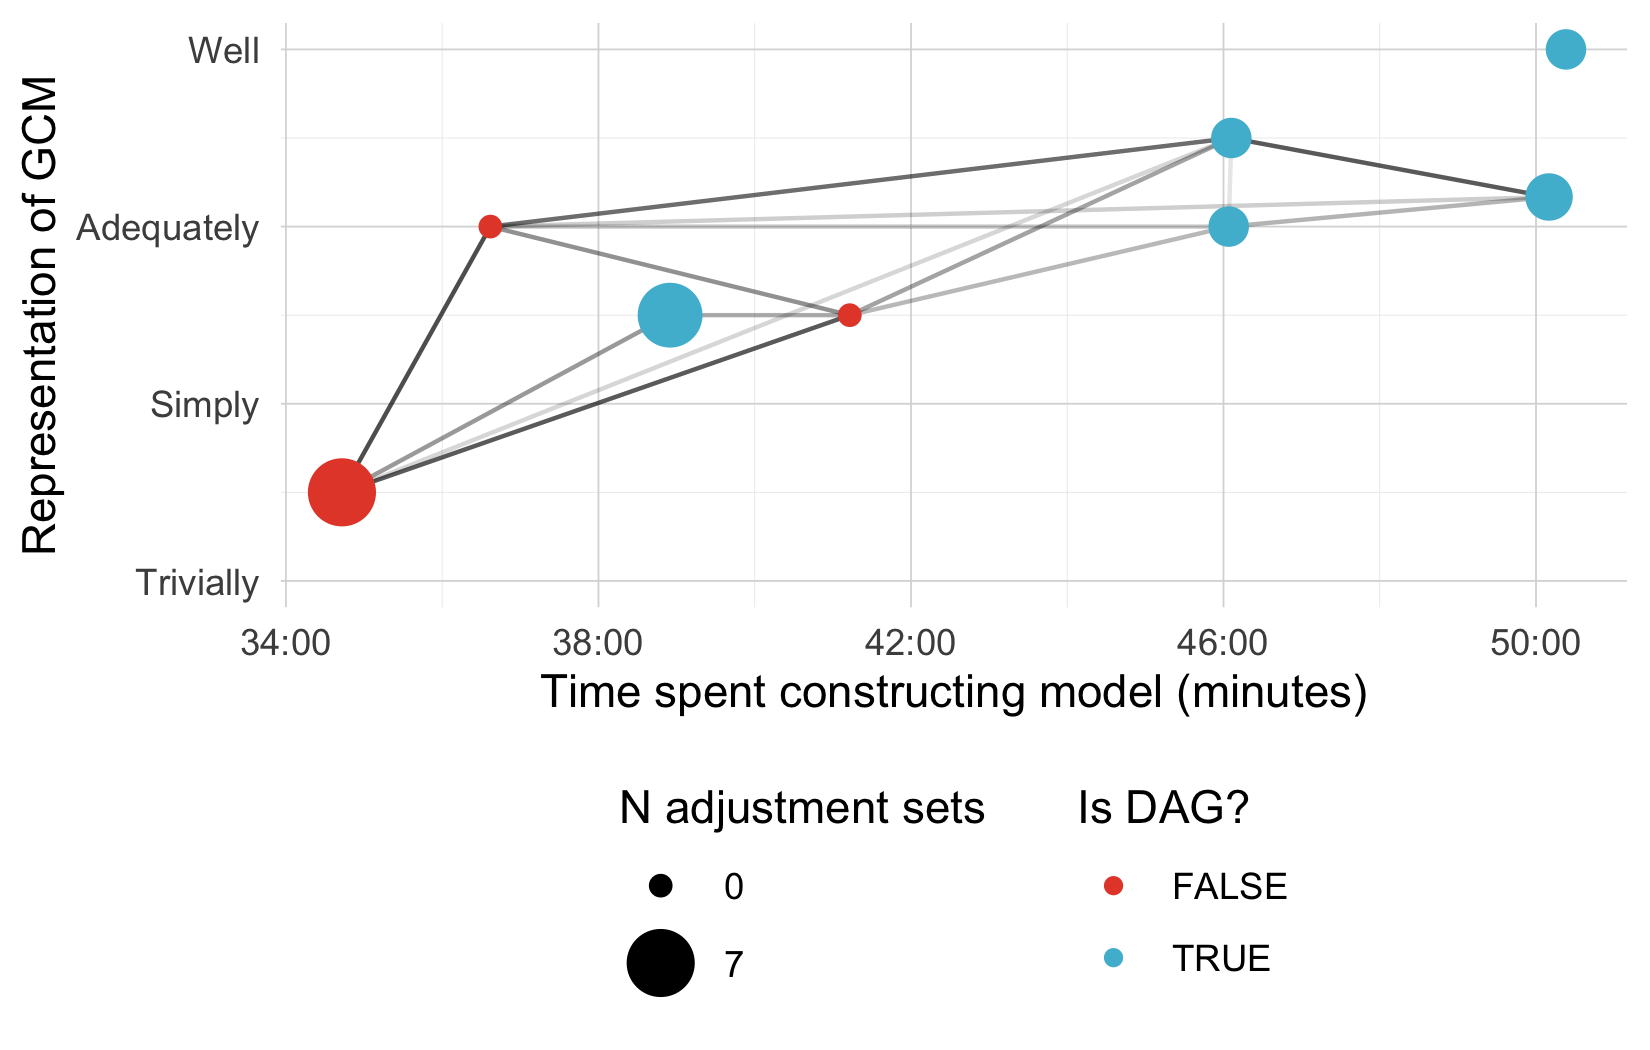
\includegraphics[keepaspectratio]{elicited-DAG-analysis_files/figure-pdf/unnamed-chunk-22-1.png}}

\begin{Shaded}
\begin{Highlighting}[]
\CommentTok{\# ggsave("figures/FIG{-}{-}time{-}modelling{-}and{-}representation{-}with{-}distances.jpg", }
\CommentTok{\#        width = 5, height = 4, }
\CommentTok{\#        dpi = 900)}
\end{Highlighting}
\end{Shaded}

\subsection{DAG networks}\label{dag-networks}

\subsubsection{Visualising model
dissimilarities}\label{visualising-model-dissimilarities}

\begin{Shaded}
\begin{Highlighting}[]
\FunctionTok{tbl\_graph}\NormalTok{(}
    \AttributeTok{nodes =}\NormalTok{ dag\_complexity\_metrics }\SpecialCharTok{|\textgreater{}} \FunctionTok{rename}\NormalTok{(}\AttributeTok{name =}\NormalTok{ Model),}
    \AttributeTok{edges =}\NormalTok{ d\_edges) }\SpecialCharTok{|\textgreater{}} 
    \FunctionTok{activate}\NormalTok{(}\StringTok{"edges"}\NormalTok{) }\SpecialCharTok{|\textgreater{}} 
    \FunctionTok{filter}\NormalTok{(edge\_d }\SpecialCharTok{\textless{}} \FloatTok{0.33}\NormalTok{) }\SpecialCharTok{|\textgreater{}} 
    \FunctionTok{ggraph}\NormalTok{(}\AttributeTok{layout =} \StringTok{"fr"}\NormalTok{) }\SpecialCharTok{+}
    \FunctionTok{geom\_edge\_fan}\NormalTok{(}\FunctionTok{aes}\NormalTok{(}\AttributeTok{alpha =}\NormalTok{ edge\_w)) }\SpecialCharTok{+}
    \FunctionTok{geom\_node\_point}\NormalTok{(}\FunctionTok{aes}\NormalTok{(}\AttributeTok{size =}\NormalTok{ density, }\AttributeTok{color =} \FunctionTok{factor}\NormalTok{(acyclic))) }\SpecialCharTok{+}
    \FunctionTok{geom\_node\_text}\NormalTok{(}\FunctionTok{aes}\NormalTok{(}\AttributeTok{label =}\NormalTok{ name), }\AttributeTok{repel =}\NormalTok{ T) }\SpecialCharTok{+}
    \FunctionTok{theme\_graph}\NormalTok{() }\SpecialCharTok{+}
    \FunctionTok{ggtitle}\NormalTok{(}\StringTok{"Graph dissimilarities"}\NormalTok{)}
\end{Highlighting}
\end{Shaded}

\pandocbounded{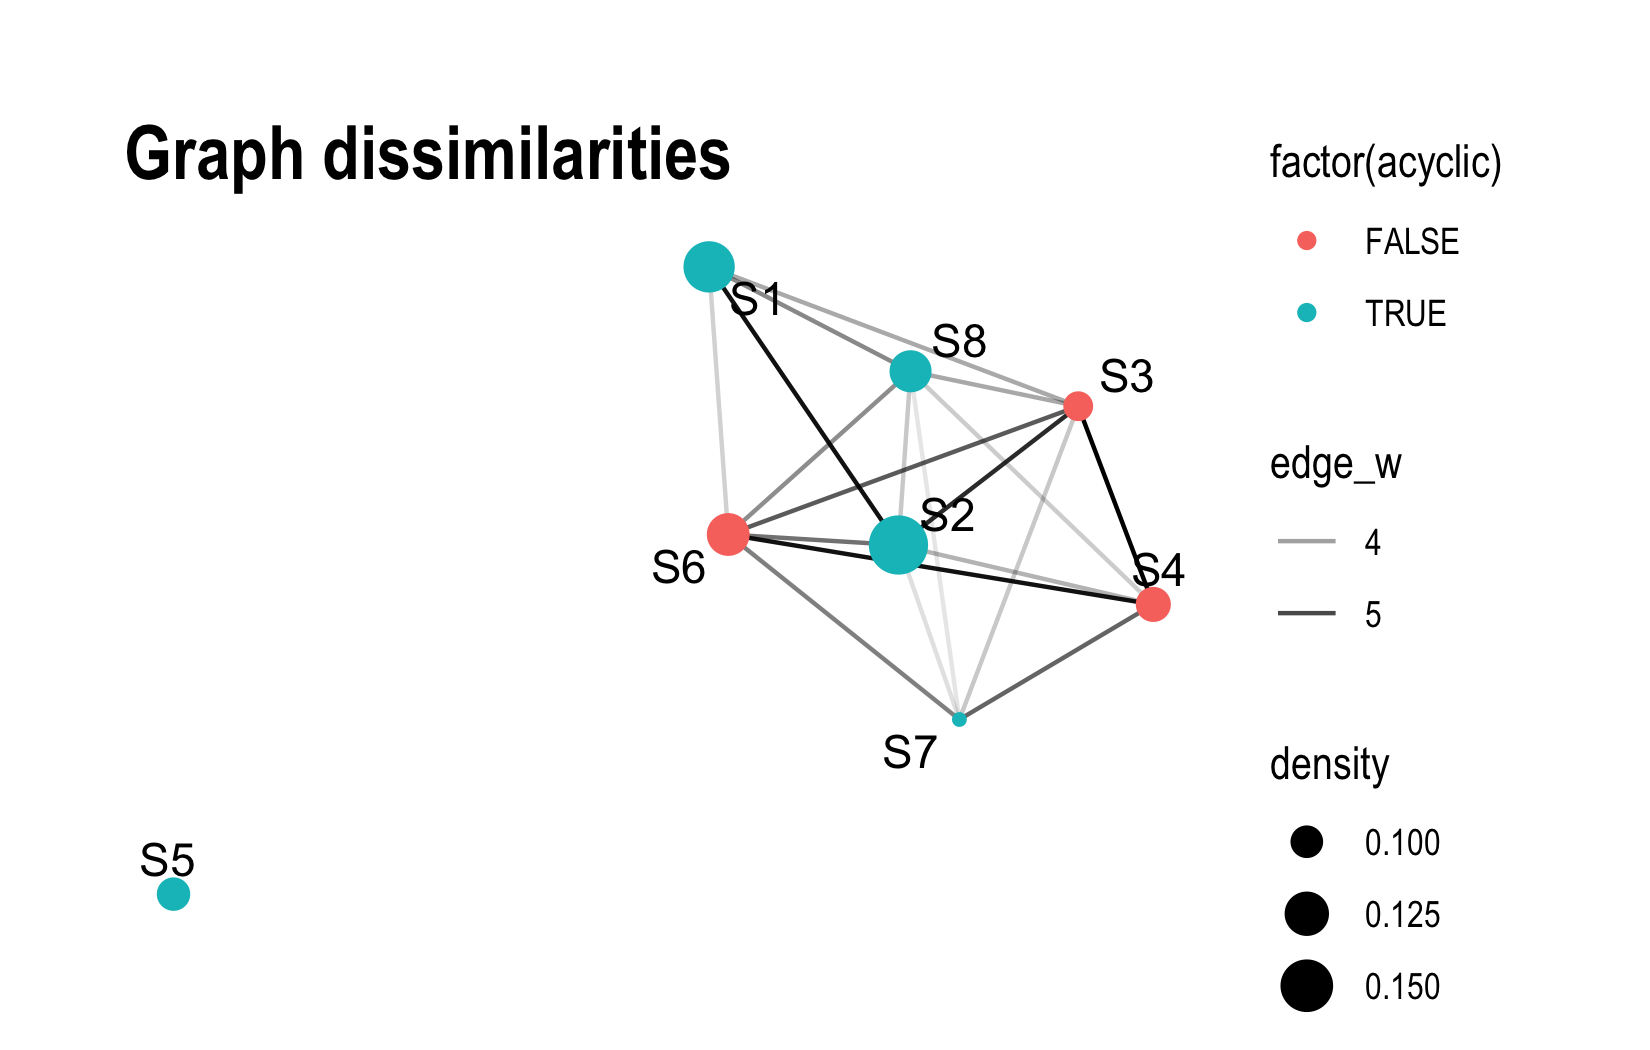
\includegraphics[keepaspectratio]{elicited-DAG-analysis_files/figure-pdf/unnamed-chunk-23-1.png}}

Same again, but hierarchical clustering

\begin{Shaded}
\begin{Highlighting}[]
\NormalTok{hc }\OtherTok{\textless{}{-}} \FunctionTok{hclust}\NormalTok{(d\_matrix }\SpecialCharTok{|\textgreater{}} \FunctionTok{select}\NormalTok{(}\SpecialCharTok{{-}}\NormalTok{from) }\SpecialCharTok{|\textgreater{}} \FunctionTok{as.dist}\NormalTok{())}
\FunctionTok{plot}\NormalTok{(hc)}
\end{Highlighting}
\end{Shaded}

\pandocbounded{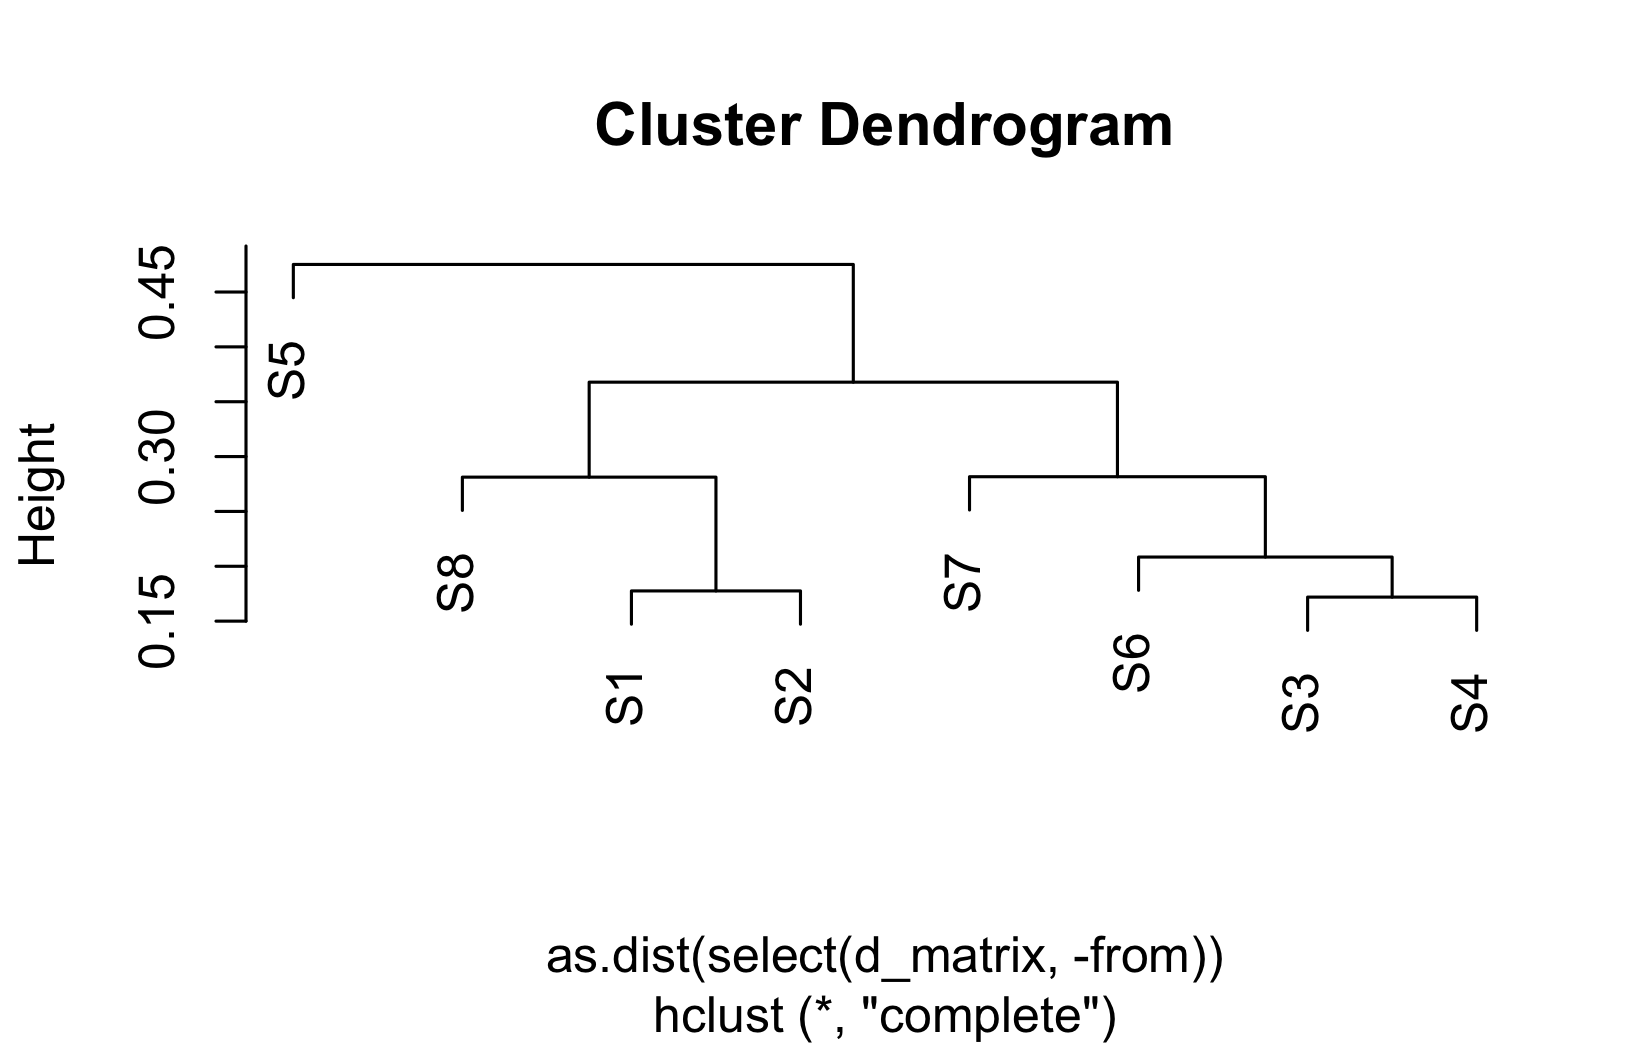
\includegraphics[keepaspectratio]{elicited-DAG-analysis_files/figure-pdf/unnamed-chunk-24-1.png}}

\subsubsection{Edge coherence}\label{edge-coherence}

\begin{Shaded}
\begin{Highlighting}[]
\NormalTok{tb\_edge\_coherence }\OtherTok{\textless{}{-}} 
\NormalTok{    edges\_with\_metrics }\SpecialCharTok{|\textgreater{}} 
    \FunctionTok{summarise}\NormalTok{(}
        \AttributeTok{n =} \FunctionTok{sum}\NormalTok{(n),}
        \AttributeTok{n\_desc =} \FunctionTok{sum}\NormalTok{(n\_desc),}
        \AttributeTok{max\_n =} \FunctionTok{sum}\NormalTok{(max\_n),}
        \AttributeTok{aligned =} \FunctionTok{mean}\NormalTok{(switched }\SpecialCharTok{==} \StringTok{"aligned"}\NormalTok{),}
        \AttributeTok{contested =} \FunctionTok{mean}\NormalTok{(switched }\SpecialCharTok{!=} \StringTok{"aligned"}\NormalTok{)}
\NormalTok{    ) }\SpecialCharTok{|\textgreater{}} 
    \FunctionTok{mutate}\NormalTok{(}\AttributeTok{edges\_included =}\NormalTok{ n }\SpecialCharTok{/}\NormalTok{ max\_n,}
           \AttributeTok{desc\_incllude =}\NormalTok{ n\_desc }\SpecialCharTok{/}\NormalTok{ max\_n)}
\NormalTok{tb\_edge\_coherence}
\end{Highlighting}
\end{Shaded}

\begin{verbatim}
# A tibble: 1 x 7
      n n_desc max_n aligned contested edges_included desc_incllude
  <int>  <int> <int>   <dbl>     <dbl>          <dbl>         <dbl>
1   204    258   258   0.938    0.0622          0.791             1
\end{verbatim}

Generally when two nodes in the model were selected by different
participants the same edge was drawn in 79.07\% of the time. A handful
of potential edges (6.22\%) were included, but asigned a different
direction of causal flow. In 100\% of the cases where a path
\(A \rightarrow B\) was included in a model, then there existed a path
from \(A\) to \(B\) in every other model that included those two nodes,
just sometimes through a mediator(s) variable.

\subsubsection{Merging graphs}\label{merging-graphs}

\begin{Shaded}
\begin{Highlighting}[]
\NormalTok{merged\_all\_graph\_layout }\OtherTok{\textless{}{-}} \FunctionTok{create\_layout}\NormalTok{(merged\_all\_graph, }\AttributeTok{layout =} \StringTok{"sugiyama"}\NormalTok{)}
\NormalTok{merged\_all\_graph\_layout\_adjusted }\OtherTok{\textless{}{-}} 
\NormalTok{    merged\_all\_graph\_layout }\SpecialCharTok{|\textgreater{}} 
    \FunctionTok{mutate}\NormalTok{(}
        \CommentTok{\# x = if\_else(name == "S.Post.Fb",x + 20,x),}
        \AttributeTok{y =} \FunctionTok{if\_else}\NormalTok{(name }\SpecialCharTok{==} \StringTok{"S.Act.Fb.Post"}\NormalTok{,y }\SpecialCharTok{+} \DecValTok{4}\NormalTok{,y)}
\NormalTok{           ) }\SpecialCharTok{|\textgreater{}} 
    \FunctionTok{mutate}\NormalTok{(}
        \AttributeTok{x =} \FunctionTok{if\_else}\NormalTok{(name }\SpecialCharTok{==} \StringTok{"S.Act"}\NormalTok{,x }\SpecialCharTok{+} \DecValTok{20}\NormalTok{,x),}
        \AttributeTok{y =} \FunctionTok{if\_else}\NormalTok{(name }\SpecialCharTok{==} \StringTok{"S.Act"}\NormalTok{,y }\SpecialCharTok{{-}} \DecValTok{4}\NormalTok{,y)}
\NormalTok{           ) }
\NormalTok{ptemp }\OtherTok{\textless{}{-}}\NormalTok{ merged\_all\_graph\_layout\_adjusted }\SpecialCharTok{|\textgreater{}} 
    \FunctionTok{ggraph}\NormalTok{() }\SpecialCharTok{+}
        \FunctionTok{geom\_edge\_fan}\NormalTok{(}\FunctionTok{aes}\NormalTok{(}\AttributeTok{alpha =}\NormalTok{ edge\_w), }\AttributeTok{strength =} \FloatTok{0.2}\NormalTok{,}
            \AttributeTok{arrow =} \FunctionTok{arrow}\NormalTok{(}\AttributeTok{length =} \FunctionTok{unit}\NormalTok{(}\DecValTok{2}\NormalTok{, }\StringTok{\textquotesingle{}mm\textquotesingle{}}\NormalTok{), }\AttributeTok{type =} \StringTok{"closed"}\NormalTok{),}
            \AttributeTok{start\_cap =} \FunctionTok{circle}\NormalTok{(}\DecValTok{3}\NormalTok{, }\StringTok{\textquotesingle{}mm\textquotesingle{}}\NormalTok{),}
            \AttributeTok{end\_cap =} \FunctionTok{circle}\NormalTok{(}\DecValTok{3}\NormalTok{, }\StringTok{\textquotesingle{}mm\textquotesingle{}}\NormalTok{)) }\SpecialCharTok{+}
        \FunctionTok{geom\_node\_point}\NormalTok{(}\FunctionTok{aes}\NormalTok{(}\AttributeTok{colour =}\NormalTok{ node\_type, }\AttributeTok{size =}\NormalTok{ node\_w)) }\SpecialCharTok{+}
        \CommentTok{\# geom\_node\_text(aes(label = name, size = node\_w, alpha = node\_w), nudge\_y = {-}.5) +}
        \FunctionTok{theme\_graph}\NormalTok{() }\SpecialCharTok{+}
        \FunctionTok{scale\_edge\_alpha\_continuous}\NormalTok{(}\AttributeTok{range =} \FunctionTok{c}\NormalTok{(}\FloatTok{0.15}\NormalTok{,}\FloatTok{0.8}\NormalTok{)) }\SpecialCharTok{+}
        \FunctionTok{scale\_alpha\_continuous}\NormalTok{(}\AttributeTok{range =} \FunctionTok{c}\NormalTok{(}\FloatTok{0.3}\NormalTok{,}\DecValTok{1}\NormalTok{)) }\SpecialCharTok{+}
        \FunctionTok{theme}\NormalTok{(}\AttributeTok{legend.position =} \StringTok{"none"}\NormalTok{)}

\NormalTok{b }\OtherTok{\textless{}{-}} \FunctionTok{ggplot\_build}\NormalTok{(ptemp)}
\NormalTok{x\_limits\_fine }\OtherTok{\textless{}{-}}\NormalTok{ b}\SpecialCharTok{$}\NormalTok{layout}\SpecialCharTok{$}\NormalTok{panel\_params[[}\DecValTok{1}\NormalTok{]]}\SpecialCharTok{$}\NormalTok{x.range}
\NormalTok{y\_limits\_fine }\OtherTok{\textless{}{-}}\NormalTok{ b}\SpecialCharTok{$}\NormalTok{layout}\SpecialCharTok{$}\NormalTok{panel\_params[[}\DecValTok{1}\NormalTok{]]}\SpecialCharTok{$}\NormalTok{y.range}



\NormalTok{plot\_fine\_graph\_from\_layout }\OtherTok{\textless{}{-}} \ControlFlowTok{function}\NormalTok{(lyt, }\AttributeTok{weight\_nodes =} \ConstantTok{TRUE}\NormalTok{) \{}
\NormalTok{    ppp }\OtherTok{\textless{}{-}} 
\NormalTok{        lyt }\SpecialCharTok{|\textgreater{}} 
        \FunctionTok{ggraph}\NormalTok{() }
    
    \ControlFlowTok{if}\NormalTok{ (weight\_nodes) \{}
\NormalTok{        pp }\OtherTok{\textless{}{-}}\NormalTok{ ppp }\SpecialCharTok{+}
            \FunctionTok{geom\_node\_point}\NormalTok{(}\FunctionTok{aes}\NormalTok{(}\AttributeTok{colour =}\NormalTok{ node\_type,}
                                \AttributeTok{size =}\NormalTok{ node\_w)) }\SpecialCharTok{+}
            \FunctionTok{scale\_size}\NormalTok{(}\AttributeTok{name =} \StringTok{"point{-}size"}\NormalTok{) }\SpecialCharTok{+}
            \FunctionTok{geom\_edge\_fan}\NormalTok{(}\FunctionTok{aes}\NormalTok{(}
                \AttributeTok{alpha =}\NormalTok{ edge\_p\_w }\SpecialCharTok{*}\NormalTok{ edge\_w }\SpecialCharTok{+}\NormalTok{ edge\_w, }
                \AttributeTok{edge\_linetype =} \FunctionTok{factor}\NormalTok{(switched)), }
                \AttributeTok{strength =} \FloatTok{0.2}\NormalTok{,}
                \AttributeTok{arrow =} \FunctionTok{arrow}\NormalTok{(}\AttributeTok{length =} \FunctionTok{unit}\NormalTok{(}\DecValTok{1}\NormalTok{, }\StringTok{\textquotesingle{}mm\textquotesingle{}}\NormalTok{),}
                              \AttributeTok{type =} \StringTok{"closed"}\NormalTok{),}
                \AttributeTok{start\_cap =} \FunctionTok{circle}\NormalTok{(}\DecValTok{3}\NormalTok{, }\StringTok{\textquotesingle{}mm\textquotesingle{}}\NormalTok{),}
                \AttributeTok{end\_cap =} \FunctionTok{circle}\NormalTok{(}\DecValTok{3}\NormalTok{, }\StringTok{\textquotesingle{}mm\textquotesingle{}}\NormalTok{))}
\NormalTok{    \} }\ControlFlowTok{else}\NormalTok{ \{}
\NormalTok{        pp }\OtherTok{\textless{}{-}}\NormalTok{ ppp }\SpecialCharTok{+}
            \FunctionTok{geom\_node\_point}\NormalTok{(}\FunctionTok{aes}\NormalTok{(}\AttributeTok{colour =}\NormalTok{ node\_type)) }\SpecialCharTok{+}
            \FunctionTok{geom\_edge\_fan}\NormalTok{(}\AttributeTok{strength =} \FloatTok{0.2}\NormalTok{, }\AttributeTok{alpha =} \FloatTok{0.5}\NormalTok{,}
                          \AttributeTok{arrow =} \FunctionTok{arrow}\NormalTok{(}\AttributeTok{length =} \FunctionTok{unit}\NormalTok{(}\DecValTok{1}\NormalTok{, }\StringTok{\textquotesingle{}mm\textquotesingle{}}\NormalTok{),}
                                        \AttributeTok{type =} \StringTok{"closed"}\NormalTok{),}
                          \AttributeTok{start\_cap =} \FunctionTok{circle}\NormalTok{(}\DecValTok{1}\NormalTok{, }\StringTok{\textquotesingle{}mm\textquotesingle{}}\NormalTok{),}
                          \AttributeTok{end\_cap =} \FunctionTok{circle}\NormalTok{(}\DecValTok{1}\NormalTok{, }\StringTok{\textquotesingle{}mm\textquotesingle{}}\NormalTok{))}
            
\NormalTok{    \}}
\NormalTok{    pp }\SpecialCharTok{+}
        \FunctionTok{scale\_colour\_okabe\_ito}\NormalTok{() }\SpecialCharTok{+}
        \CommentTok{\# geom\_node\_text(aes(label = name, size = node\_w, alpha = node\_w), nudge\_y = {-}.5) +}
        \FunctionTok{theme\_graph}\NormalTok{() }\SpecialCharTok{+}
        \FunctionTok{scale\_edge\_alpha\_continuous}\NormalTok{(}\AttributeTok{range =} \FunctionTok{c}\NormalTok{(}\FloatTok{0.15}\NormalTok{,}\FloatTok{0.8}\NormalTok{)) }\SpecialCharTok{+}
        \FunctionTok{scale\_alpha\_continuous}\NormalTok{(}\AttributeTok{range =} \FunctionTok{c}\NormalTok{(}\FloatTok{0.3}\NormalTok{,}\DecValTok{1}\NormalTok{)) }\SpecialCharTok{+}
        \FunctionTok{theme}\NormalTok{(}\AttributeTok{legend.position =} \StringTok{"none"}\NormalTok{,}
              \AttributeTok{plot.margin =} \FunctionTok{margin}\NormalTok{(}\AttributeTok{t =} \DecValTok{0}\NormalTok{, }\AttributeTok{r =} \DecValTok{0}\NormalTok{, }\AttributeTok{b =} \DecValTok{0}\NormalTok{, }\AttributeTok{l =} \DecValTok{0}\NormalTok{, }\AttributeTok{unit =} \StringTok{"pt"}\NormalTok{)) }\SpecialCharTok{+}
        \FunctionTok{xlim}\NormalTok{(x\_limits\_fine) }\SpecialCharTok{+}
        \FunctionTok{ylim}\NormalTok{(y\_limits\_fine)}
\NormalTok{\}}

\NormalTok{g\_plot\_fine }\OtherTok{\textless{}{-}} \ControlFlowTok{function}\NormalTok{(g, }\AttributeTok{lyt =}\NormalTok{ merged\_all\_graph\_layout\_adjusted, }\AttributeTok{weight\_nodes =} \ConstantTok{TRUE}\NormalTok{) \{}
    \FunctionTok{create\_layout}\NormalTok{(g, }\AttributeTok{layout =} \StringTok{"sugiyama"}\NormalTok{) }\SpecialCharTok{|\textgreater{}} 
        \FunctionTok{left\_join}\NormalTok{(lyt }\SpecialCharTok{|\textgreater{}} \FunctionTok{select}\NormalTok{(x,y,name,node\_group,node\_type,node\_w), }\AttributeTok{by =} \StringTok{"name"}\NormalTok{,}
                  \AttributeTok{suffix =} \FunctionTok{c}\NormalTok{(}\StringTok{".default"}\NormalTok{, }\StringTok{""}\NormalTok{)) }\SpecialCharTok{|\textgreater{}} 
        \FunctionTok{plot\_fine\_graph\_from\_layout}\NormalTok{(}\AttributeTok{weight\_nodes =}\NormalTok{ weight\_nodes)}
\NormalTok{\}}

\NormalTok{pMergedFineLegend }\OtherTok{\textless{}{-}}\NormalTok{ merged\_all\_graph\_layout\_adjusted }\SpecialCharTok{|\textgreater{}} 
    \FunctionTok{g\_plot\_fine}\NormalTok{() }\SpecialCharTok{+} 
    \FunctionTok{theme}\NormalTok{(}\AttributeTok{legend.position =} \StringTok{"bottom"}\NormalTok{) }\SpecialCharTok{+}
    \FunctionTok{guides}\NormalTok{(}\AttributeTok{size =} \StringTok{"none"}\NormalTok{, }\AttributeTok{edge\_width =} \StringTok{"none"}\NormalTok{, }\AttributeTok{alpha =} \StringTok{"none"}\NormalTok{, }\AttributeTok{edge\_alpha =} \StringTok{"none"}\NormalTok{,}
           \AttributeTok{color =} \FunctionTok{guide\_legend}\NormalTok{(}\AttributeTok{nrow =} \DecValTok{1}\NormalTok{)) }\SpecialCharTok{+}
    \FunctionTok{theme}\NormalTok{(}\AttributeTok{legend.title =} \FunctionTok{element\_blank}\NormalTok{())}
\NormalTok{pMergedFineLegend}
\end{Highlighting}
\end{Shaded}

\pandocbounded{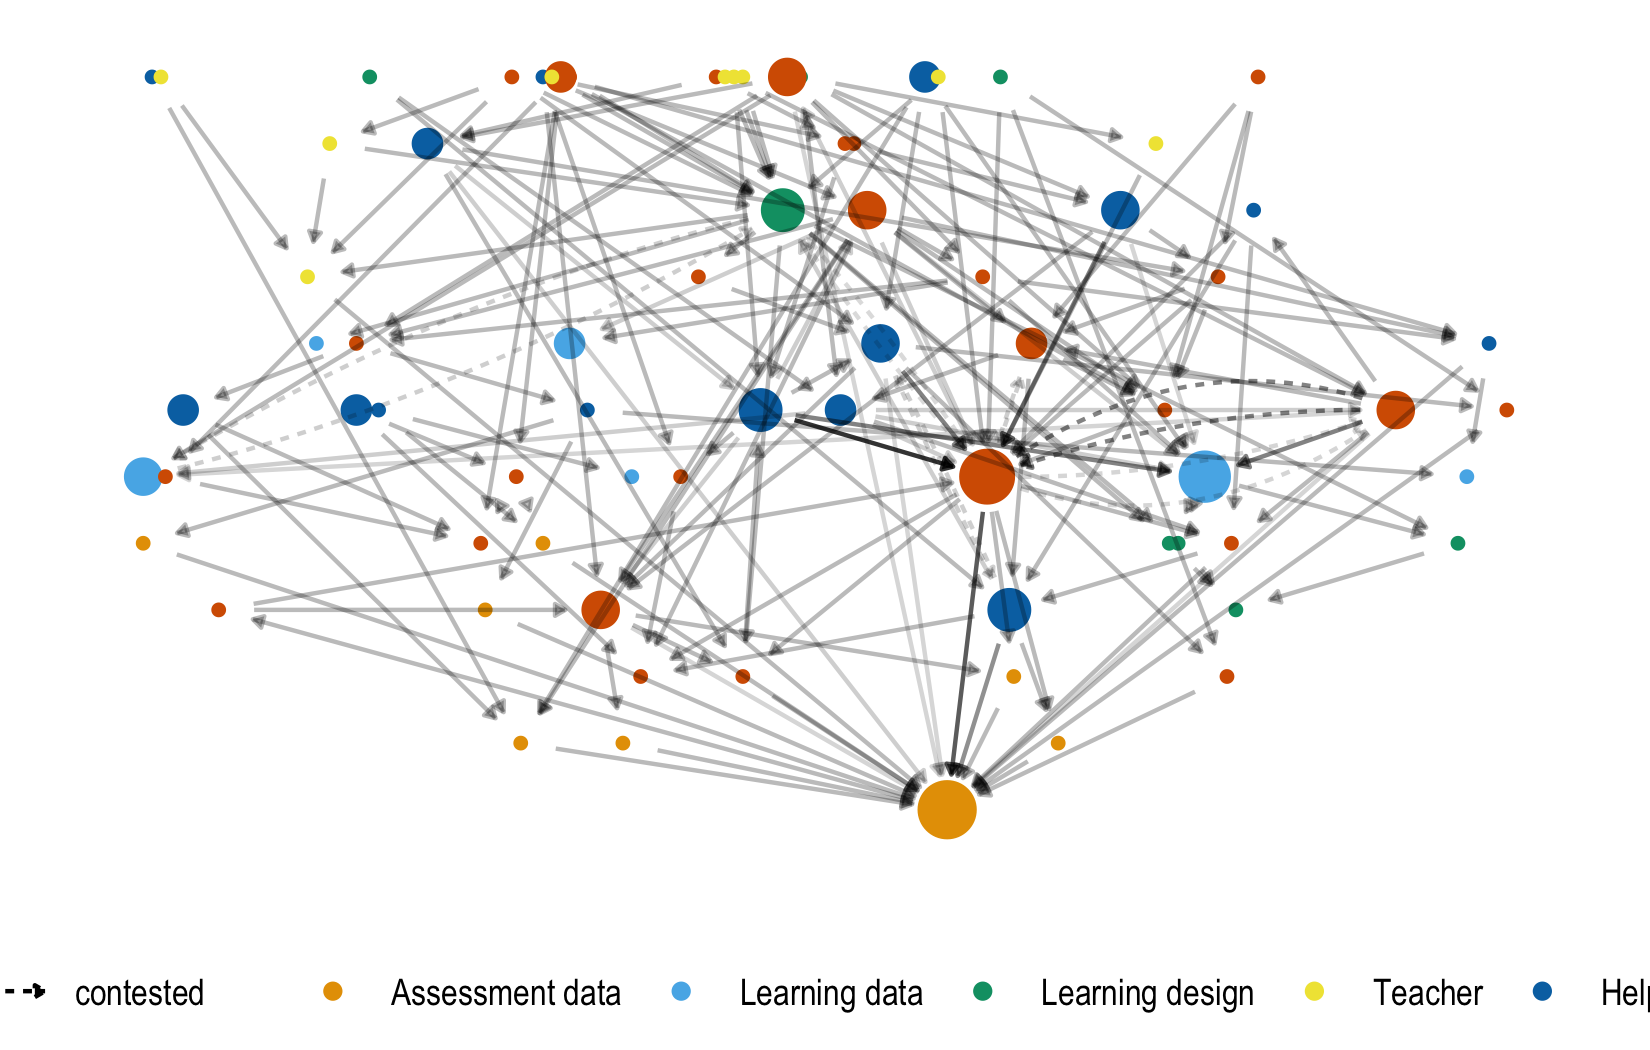
\includegraphics[keepaspectratio]{elicited-DAG-analysis_files/figure-pdf/plotting-merged-graph-1.png}}

\begin{Shaded}
\begin{Highlighting}[]
\NormalTok{pMergedFineLegendTall }\OtherTok{\textless{}{-}}\NormalTok{ merged\_all\_graph\_layout\_adjusted }\SpecialCharTok{|\textgreater{}} 
    \FunctionTok{g\_plot\_fine}\NormalTok{() }\SpecialCharTok{+} 
    \FunctionTok{theme}\NormalTok{(}\AttributeTok{legend.position =} \StringTok{"right"}\NormalTok{) }\SpecialCharTok{+}
    \FunctionTok{guides}\NormalTok{(}\AttributeTok{size =} \StringTok{"none"}\NormalTok{, }\AttributeTok{alpha =} \StringTok{"none"}\NormalTok{, }\AttributeTok{edge\_alpha =} \StringTok{"none"}\NormalTok{, }\AttributeTok{edge\_width =} \StringTok{"none"}\NormalTok{,}
           \AttributeTok{color =} \FunctionTok{guide\_legend}\NormalTok{(}\AttributeTok{ncol =} \DecValTok{2}\NormalTok{)) }\SpecialCharTok{+}
    \FunctionTok{theme}\NormalTok{(}\AttributeTok{legend.title =} \FunctionTok{element\_blank}\NormalTok{())}
\NormalTok{pMergedFine }\OtherTok{\textless{}{-}}\NormalTok{ pMergedFineLegend }\SpecialCharTok{+}
    \FunctionTok{theme}\NormalTok{(}\AttributeTok{legend.position =} \StringTok{"none"}\NormalTok{)}

\NormalTok{pMergedFineLabelled }\OtherTok{\textless{}{-}}\NormalTok{ pMergedFine }\SpecialCharTok{+} 
    \FunctionTok{geom\_node\_text}\NormalTok{(}
        \FunctionTok{aes}\NormalTok{(}\AttributeTok{label =}\NormalTok{ nice\_name, }\AttributeTok{size =}\NormalTok{ node\_w, }\AttributeTok{colour =}\NormalTok{ node\_type), }\AttributeTok{alpha =} \FloatTok{0.6}\NormalTok{, }
        \AttributeTok{data =}\NormalTok{ merged\_all\_graph\_layout\_adjusted }\SpecialCharTok{|\textgreater{}}  \FunctionTok{filter}\NormalTok{(node\_w }\SpecialCharTok{\textgreater{}} \DecValTok{0}\NormalTok{), }\AttributeTok{repel =} \ConstantTok{TRUE}\NormalTok{, }\AttributeTok{max.overlaps =} \DecValTok{4}\NormalTok{) }\SpecialCharTok{+}
\NormalTok{    ggnewscale}\SpecialCharTok{::}\FunctionTok{new\_scale}\NormalTok{(}\StringTok{"size"}\NormalTok{) }\SpecialCharTok{+}
    \FunctionTok{scale\_size}\NormalTok{(}\AttributeTok{range =} \FunctionTok{c}\NormalTok{(}\DecValTok{3}\NormalTok{,}\DecValTok{6}\NormalTok{), }\AttributeTok{name =} \StringTok{"text{-}size"}\NormalTok{)}
\NormalTok{pMergedFineLabelled}
\end{Highlighting}
\end{Shaded}

\begin{verbatim}
Warning: ggrepel: 22 unlabeled data points (too many overlaps). Consider
increasing max.overlaps
\end{verbatim}

\pandocbounded{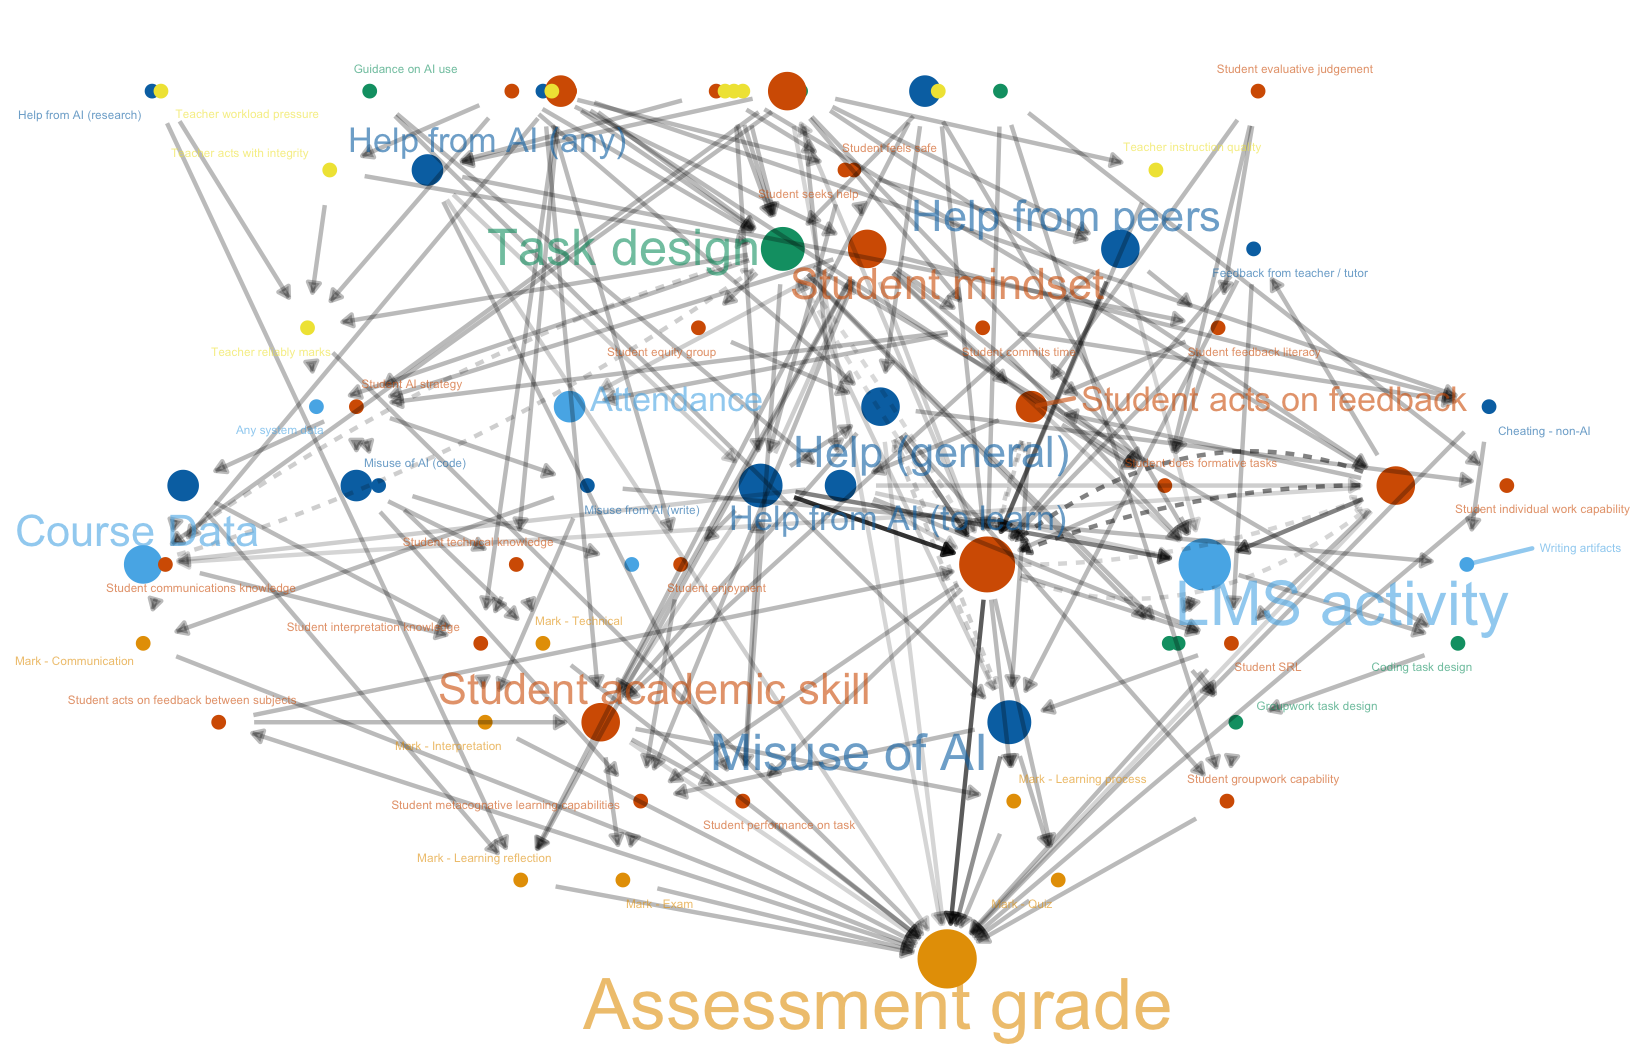
\includegraphics[keepaspectratio]{elicited-DAG-analysis_files/figure-pdf/plotting-merged-graph-2.png}}

\begin{Shaded}
\begin{Highlighting}[]
\CommentTok{\# Extract legend}
\NormalTok{leg }\OtherTok{\textless{}{-}}\NormalTok{ cowplot}\SpecialCharTok{::}\FunctionTok{get\_legend}\NormalTok{(pMergedFineLegend)}
\end{Highlighting}
\end{Shaded}

\begin{verbatim}
Warning in grid.Call(C_stringMetric, as.graphicsAnnot(x$label)): font family
'Arial Narrow' not found in PostScript font database
\end{verbatim}

\begin{verbatim}
Warning in grid.Call(C_stringMetric, as.graphicsAnnot(x$label)): font family
'Arial Narrow' not found in PostScript font database
Warning in grid.Call(C_stringMetric, as.graphicsAnnot(x$label)): font family
'Arial Narrow' not found in PostScript font database
Warning in grid.Call(C_stringMetric, as.graphicsAnnot(x$label)): font family
'Arial Narrow' not found in PostScript font database
Warning in grid.Call(C_stringMetric, as.graphicsAnnot(x$label)): font family
'Arial Narrow' not found in PostScript font database
Warning in grid.Call(C_stringMetric, as.graphicsAnnot(x$label)): font family
'Arial Narrow' not found in PostScript font database
Warning in grid.Call(C_stringMetric, as.graphicsAnnot(x$label)): font family
'Arial Narrow' not found in PostScript font database
Warning in grid.Call(C_stringMetric, as.graphicsAnnot(x$label)): font family
'Arial Narrow' not found in PostScript font database
Warning in grid.Call(C_stringMetric, as.graphicsAnnot(x$label)): font family
'Arial Narrow' not found in PostScript font database
Warning in grid.Call(C_stringMetric, as.graphicsAnnot(x$label)): font family
'Arial Narrow' not found in PostScript font database
Warning in grid.Call(C_stringMetric, as.graphicsAnnot(x$label)): font family
'Arial Narrow' not found in PostScript font database
Warning in grid.Call(C_stringMetric, as.graphicsAnnot(x$label)): font family
'Arial Narrow' not found in PostScript font database
Warning in grid.Call(C_stringMetric, as.graphicsAnnot(x$label)): font family
'Arial Narrow' not found in PostScript font database
Warning in grid.Call(C_stringMetric, as.graphicsAnnot(x$label)): font family
'Arial Narrow' not found in PostScript font database
\end{verbatim}

\begin{verbatim}
Warning in grid.Call(C_textBounds, as.graphicsAnnot(x$label), x$x, x$y, : font
family 'Arial Narrow' not found in PostScript font database
Warning in grid.Call(C_textBounds, as.graphicsAnnot(x$label), x$x, x$y, : font
family 'Arial Narrow' not found in PostScript font database
Warning in grid.Call(C_textBounds, as.graphicsAnnot(x$label), x$x, x$y, : font
family 'Arial Narrow' not found in PostScript font database
Warning in grid.Call(C_textBounds, as.graphicsAnnot(x$label), x$x, x$y, : font
family 'Arial Narrow' not found in PostScript font database
Warning in grid.Call(C_textBounds, as.graphicsAnnot(x$label), x$x, x$y, : font
family 'Arial Narrow' not found in PostScript font database
Warning in grid.Call(C_textBounds, as.graphicsAnnot(x$label), x$x, x$y, : font
family 'Arial Narrow' not found in PostScript font database
Warning in grid.Call(C_textBounds, as.graphicsAnnot(x$label), x$x, x$y, : font
family 'Arial Narrow' not found in PostScript font database
Warning in grid.Call(C_textBounds, as.graphicsAnnot(x$label), x$x, x$y, : font
family 'Arial Narrow' not found in PostScript font database
Warning in grid.Call(C_textBounds, as.graphicsAnnot(x$label), x$x, x$y, : font
family 'Arial Narrow' not found in PostScript font database
Warning in grid.Call(C_textBounds, as.graphicsAnnot(x$label), x$x, x$y, : font
family 'Arial Narrow' not found in PostScript font database
Warning in grid.Call(C_textBounds, as.graphicsAnnot(x$label), x$x, x$y, : font
family 'Arial Narrow' not found in PostScript font database
Warning in grid.Call(C_textBounds, as.graphicsAnnot(x$label), x$x, x$y, : font
family 'Arial Narrow' not found in PostScript font database
Warning in grid.Call(C_textBounds, as.graphicsAnnot(x$label), x$x, x$y, : font
family 'Arial Narrow' not found in PostScript font database
Warning in grid.Call(C_textBounds, as.graphicsAnnot(x$label), x$x, x$y, : font
family 'Arial Narrow' not found in PostScript font database
Warning in grid.Call(C_textBounds, as.graphicsAnnot(x$label), x$x, x$y, : font
family 'Arial Narrow' not found in PostScript font database
Warning in grid.Call(C_textBounds, as.graphicsAnnot(x$label), x$x, x$y, : font
family 'Arial Narrow' not found in PostScript font database
Warning in grid.Call(C_textBounds, as.graphicsAnnot(x$label), x$x, x$y, : font
family 'Arial Narrow' not found in PostScript font database
Warning in grid.Call(C_textBounds, as.graphicsAnnot(x$label), x$x, x$y, : font
family 'Arial Narrow' not found in PostScript font database
Warning in grid.Call(C_textBounds, as.graphicsAnnot(x$label), x$x, x$y, : font
family 'Arial Narrow' not found in PostScript font database
Warning in grid.Call(C_textBounds, as.graphicsAnnot(x$label), x$x, x$y, : font
family 'Arial Narrow' not found in PostScript font database
Warning in grid.Call(C_textBounds, as.graphicsAnnot(x$label), x$x, x$y, : font
family 'Arial Narrow' not found in PostScript font database
Warning in grid.Call(C_textBounds, as.graphicsAnnot(x$label), x$x, x$y, : font
family 'Arial Narrow' not found in PostScript font database
Warning in grid.Call(C_textBounds, as.graphicsAnnot(x$label), x$x, x$y, : font
family 'Arial Narrow' not found in PostScript font database
Warning in grid.Call(C_textBounds, as.graphicsAnnot(x$label), x$x, x$y, : font
family 'Arial Narrow' not found in PostScript font database
\end{verbatim}

\begin{Shaded}
\begin{Highlighting}[]
\CommentTok{\# Turn it into a ggplot object for saving}
\NormalTok{legplot }\OtherTok{\textless{}{-}}\NormalTok{ cowplot}\SpecialCharTok{::}\FunctionTok{ggdraw}\NormalTok{(leg)}
\CommentTok{\# Save just the legend}
\FunctionTok{ggsave}\NormalTok{(}\StringTok{"dag\_legend.jpg"}\NormalTok{, legplot, }\AttributeTok{width =} \DecValTok{6}\NormalTok{, }\AttributeTok{height =} \DecValTok{1}\NormalTok{)}

\NormalTok{leg\_tall }\OtherTok{\textless{}{-}}\NormalTok{ cowplot}\SpecialCharTok{::}\FunctionTok{get\_legend}\NormalTok{(pMergedFineLegendTall)}
\end{Highlighting}
\end{Shaded}

\begin{verbatim}
Warning in grid.Call(C_textBounds, as.graphicsAnnot(x$label), x$x, x$y, : font
family 'Arial Narrow' not found in PostScript font database
Warning in grid.Call(C_textBounds, as.graphicsAnnot(x$label), x$x, x$y, : font
family 'Arial Narrow' not found in PostScript font database
Warning in grid.Call(C_textBounds, as.graphicsAnnot(x$label), x$x, x$y, : font
family 'Arial Narrow' not found in PostScript font database
Warning in grid.Call(C_textBounds, as.graphicsAnnot(x$label), x$x, x$y, : font
family 'Arial Narrow' not found in PostScript font database
Warning in grid.Call(C_textBounds, as.graphicsAnnot(x$label), x$x, x$y, : font
family 'Arial Narrow' not found in PostScript font database
Warning in grid.Call(C_textBounds, as.graphicsAnnot(x$label), x$x, x$y, : font
family 'Arial Narrow' not found in PostScript font database
Warning in grid.Call(C_textBounds, as.graphicsAnnot(x$label), x$x, x$y, : font
family 'Arial Narrow' not found in PostScript font database
Warning in grid.Call(C_textBounds, as.graphicsAnnot(x$label), x$x, x$y, : font
family 'Arial Narrow' not found in PostScript font database
Warning in grid.Call(C_textBounds, as.graphicsAnnot(x$label), x$x, x$y, : font
family 'Arial Narrow' not found in PostScript font database
Warning in grid.Call(C_textBounds, as.graphicsAnnot(x$label), x$x, x$y, : font
family 'Arial Narrow' not found in PostScript font database
Warning in grid.Call(C_textBounds, as.graphicsAnnot(x$label), x$x, x$y, : font
family 'Arial Narrow' not found in PostScript font database
Warning in grid.Call(C_textBounds, as.graphicsAnnot(x$label), x$x, x$y, : font
family 'Arial Narrow' not found in PostScript font database
Warning in grid.Call(C_textBounds, as.graphicsAnnot(x$label), x$x, x$y, : font
family 'Arial Narrow' not found in PostScript font database
Warning in grid.Call(C_textBounds, as.graphicsAnnot(x$label), x$x, x$y, : font
family 'Arial Narrow' not found in PostScript font database
Warning in grid.Call(C_textBounds, as.graphicsAnnot(x$label), x$x, x$y, : font
family 'Arial Narrow' not found in PostScript font database
Warning in grid.Call(C_textBounds, as.graphicsAnnot(x$label), x$x, x$y, : font
family 'Arial Narrow' not found in PostScript font database
Warning in grid.Call(C_textBounds, as.graphicsAnnot(x$label), x$x, x$y, : font
family 'Arial Narrow' not found in PostScript font database
\end{verbatim}

\begin{Shaded}
\begin{Highlighting}[]
\NormalTok{leg\_tall\_plot }\OtherTok{\textless{}{-}}\NormalTok{ cowplot}\SpecialCharTok{::}\FunctionTok{ggdraw}\NormalTok{(leg\_tall)}


\CommentTok{\# ggsave("dag\_merged\_fine.svg", pMergedFine, width = 6, height = 4)}
\CommentTok{\# ggsave("dag\_merged\_fine\_labelled.svg", pMergedFineLabelled, width = 6, height = 4)}
\end{Highlighting}
\end{Shaded}

\begin{Shaded}
\begin{Highlighting}[]
\NormalTok{p1 }\OtherTok{\textless{}{-}} \FunctionTok{g\_plot\_fine}\NormalTok{(tdag\_s1, }\AttributeTok{weight\_nodes =} \ConstantTok{FALSE}\NormalTok{)}
\NormalTok{p2 }\OtherTok{\textless{}{-}} \FunctionTok{g\_plot\_fine}\NormalTok{(tdag\_s2, }\AttributeTok{weight\_nodes =} \ConstantTok{FALSE}\NormalTok{)}
\NormalTok{p3 }\OtherTok{\textless{}{-}} \FunctionTok{g\_plot\_fine}\NormalTok{(tdag\_s3, }\AttributeTok{weight\_nodes =} \ConstantTok{FALSE}\NormalTok{)}
\NormalTok{p4 }\OtherTok{\textless{}{-}} \FunctionTok{g\_plot\_fine}\NormalTok{(tdag\_s4, }\AttributeTok{weight\_nodes =} \ConstantTok{FALSE}\NormalTok{)}
\NormalTok{p5 }\OtherTok{\textless{}{-}} \FunctionTok{g\_plot\_fine}\NormalTok{(tdag\_s5, }\AttributeTok{weight\_nodes =} \ConstantTok{FALSE}\NormalTok{)}
\NormalTok{p6 }\OtherTok{\textless{}{-}} \FunctionTok{g\_plot\_fine}\NormalTok{(tdag\_s6, }\AttributeTok{weight\_nodes =} \ConstantTok{FALSE}\NormalTok{)}
\NormalTok{p7 }\OtherTok{\textless{}{-}} \FunctionTok{g\_plot\_fine}\NormalTok{(tdag\_s7, }\AttributeTok{weight\_nodes =} \ConstantTok{FALSE}\NormalTok{)}
\NormalTok{p8 }\OtherTok{\textless{}{-}} \FunctionTok{g\_plot\_fine}\NormalTok{(tdag\_s8, }\AttributeTok{weight\_nodes =} \ConstantTok{FALSE}\NormalTok{)}

\CommentTok{\# Plot border }
    \CommentTok{\# theme(}
    \CommentTok{\#   plot.background = element\_rect(}
    \CommentTok{\#     colour = "grey70", }
    \CommentTok{\#     fill = NA,}
    \CommentTok{\#     linewidth = 1}
    \CommentTok{\#   )}
    \CommentTok{\# )}

\NormalTok{hl\_text\_size }\OtherTok{\textless{}{-}} \FloatTok{1.5}
\NormalTok{hl\_text\_alpha }\OtherTok{\textless{}{-}} \FloatTok{0.7}

\NormalTok{p2peerHighlight }\OtherTok{\textless{}{-}}\NormalTok{ p2 }\SpecialCharTok{+} 
    \FunctionTok{geom\_node\_point}\NormalTok{(}\AttributeTok{size =} \DecValTok{3}\NormalTok{, }\AttributeTok{shape =} \DecValTok{1}\NormalTok{, }\AttributeTok{alpha =} \FloatTok{0.6}\NormalTok{,}
    \AttributeTok{data =}\NormalTok{ p2}\SpecialCharTok{$}\NormalTok{data }\SpecialCharTok{|\textgreater{}}  \FunctionTok{filter}\NormalTok{(name }\SpecialCharTok{==} \StringTok{"H.Peer"}\NormalTok{)) }\SpecialCharTok{+}
    \FunctionTok{geom\_node\_point}\NormalTok{(}\AttributeTok{size =} \DecValTok{5}\NormalTok{, }\AttributeTok{shape =} \DecValTok{1}\NormalTok{, }\AttributeTok{alpha =} \FloatTok{0.3}\NormalTok{,}
    \AttributeTok{data =}\NormalTok{ p2}\SpecialCharTok{$}\NormalTok{data }\SpecialCharTok{|\textgreater{}}  \FunctionTok{filter}\NormalTok{(name }\SpecialCharTok{==} \StringTok{"H.Peer"}\NormalTok{)) }\SpecialCharTok{+}
    \FunctionTok{geom\_node\_point}\NormalTok{(}\AttributeTok{size =} \DecValTok{7}\NormalTok{, }\AttributeTok{shape =} \DecValTok{1}\NormalTok{, }\AttributeTok{alpha =} \FloatTok{0.1}\NormalTok{,}
    \AttributeTok{data =}\NormalTok{ p2}\SpecialCharTok{$}\NormalTok{data }\SpecialCharTok{|\textgreater{}}  \FunctionTok{filter}\NormalTok{(name }\SpecialCharTok{==} \StringTok{"H.Peer"}\NormalTok{)) }\SpecialCharTok{+}
    \FunctionTok{geom\_node\_text}\NormalTok{(}\FunctionTok{aes}\NormalTok{(}\AttributeTok{label =}\NormalTok{ nice\_name, }\AttributeTok{colour =}\NormalTok{ node\_type), }
                   \AttributeTok{size =}\NormalTok{ hl\_text\_size , }\AttributeTok{alpha =}\NormalTok{ hl\_text\_alpha,}
    \AttributeTok{data =}\NormalTok{ p2}\SpecialCharTok{$}\NormalTok{data }\SpecialCharTok{|\textgreater{}}  \FunctionTok{filter}\NormalTok{(name }\SpecialCharTok{==} \StringTok{"H.Peer"}\NormalTok{) }\SpecialCharTok{|\textgreater{}} 
        \FunctionTok{inner\_join}\NormalTok{(name\_node\_nice\_name, }\AttributeTok{by =} \StringTok{"name"}\NormalTok{), }\AttributeTok{repel =}\NormalTok{ T) }
\NormalTok{p3peerHighlight }\OtherTok{\textless{}{-}}\NormalTok{ p3 }\SpecialCharTok{+} 
    \FunctionTok{geom\_node\_point}\NormalTok{(}\AttributeTok{size =} \DecValTok{3}\NormalTok{, }\AttributeTok{shape =} \DecValTok{1}\NormalTok{, }\AttributeTok{alpha =} \FloatTok{0.6}\NormalTok{,}
    \AttributeTok{data =}\NormalTok{ p3}\SpecialCharTok{$}\NormalTok{data }\SpecialCharTok{|\textgreater{}}  \FunctionTok{filter}\NormalTok{(name }\SpecialCharTok{==} \StringTok{"H.Peer"}\NormalTok{)) }\SpecialCharTok{+}
    \FunctionTok{geom\_node\_point}\NormalTok{(}\AttributeTok{size =} \DecValTok{5}\NormalTok{, }\AttributeTok{shape =} \DecValTok{1}\NormalTok{, }\AttributeTok{alpha =} \FloatTok{0.3}\NormalTok{,}
    \AttributeTok{data =}\NormalTok{ p3}\SpecialCharTok{$}\NormalTok{data }\SpecialCharTok{|\textgreater{}}  \FunctionTok{filter}\NormalTok{(name }\SpecialCharTok{==} \StringTok{"H.Peer"}\NormalTok{)) }\SpecialCharTok{+}
    \FunctionTok{geom\_node\_point}\NormalTok{(}\AttributeTok{size =} \DecValTok{7}\NormalTok{, }\AttributeTok{shape =} \DecValTok{1}\NormalTok{, }\AttributeTok{alpha =} \FloatTok{0.1}\NormalTok{,}
    \AttributeTok{data =}\NormalTok{ p3}\SpecialCharTok{$}\NormalTok{data }\SpecialCharTok{|\textgreater{}}  \FunctionTok{filter}\NormalTok{(name }\SpecialCharTok{==} \StringTok{"H.Peer"}\NormalTok{)) }\SpecialCharTok{+}
    \FunctionTok{geom\_node\_text}\NormalTok{(}\FunctionTok{aes}\NormalTok{(}\AttributeTok{label =}\NormalTok{ nice\_name, }\AttributeTok{colour =}\NormalTok{ node\_type), }
                   \AttributeTok{size =}\NormalTok{ hl\_text\_size , }\AttributeTok{alpha =}\NormalTok{ hl\_text\_alpha,}
    \AttributeTok{data =}\NormalTok{ p3}\SpecialCharTok{$}\NormalTok{data }\SpecialCharTok{|\textgreater{}}  \FunctionTok{filter}\NormalTok{(name }\SpecialCharTok{==} \StringTok{"H.Peer"}\NormalTok{) }\SpecialCharTok{|\textgreater{}} 
        \FunctionTok{inner\_join}\NormalTok{(name\_node\_nice\_name, }\AttributeTok{by =} \StringTok{"name"}\NormalTok{), }\AttributeTok{repel =}\NormalTok{ T) }
\NormalTok{p4peerHighlight }\OtherTok{\textless{}{-}}\NormalTok{ p4 }\SpecialCharTok{+}
    \FunctionTok{geom\_node\_point}\NormalTok{(}\AttributeTok{size =} \DecValTok{3}\NormalTok{, }\AttributeTok{shape =} \DecValTok{1}\NormalTok{, }\AttributeTok{alpha =} \FloatTok{0.6}\NormalTok{,}
    \AttributeTok{data =}\NormalTok{ p4}\SpecialCharTok{$}\NormalTok{data }\SpecialCharTok{|\textgreater{}}  \FunctionTok{filter}\NormalTok{(name }\SpecialCharTok{==} \StringTok{"H.Peer"}\NormalTok{)) }\SpecialCharTok{+}
    \FunctionTok{geom\_node\_point}\NormalTok{(}\AttributeTok{size =} \DecValTok{5}\NormalTok{, }\AttributeTok{shape =} \DecValTok{1}\NormalTok{, }\AttributeTok{alpha =} \FloatTok{0.3}\NormalTok{,}
    \AttributeTok{data =}\NormalTok{ p4}\SpecialCharTok{$}\NormalTok{data }\SpecialCharTok{|\textgreater{}}  \FunctionTok{filter}\NormalTok{(name }\SpecialCharTok{==} \StringTok{"H.Peer"}\NormalTok{)) }\SpecialCharTok{+}
    \FunctionTok{geom\_node\_point}\NormalTok{(}\AttributeTok{size =} \DecValTok{7}\NormalTok{, }\AttributeTok{shape =} \DecValTok{1}\NormalTok{, }\AttributeTok{alpha =} \FloatTok{0.1}\NormalTok{,}
    \AttributeTok{data =}\NormalTok{ p4}\SpecialCharTok{$}\NormalTok{data }\SpecialCharTok{|\textgreater{}}  \FunctionTok{filter}\NormalTok{(name }\SpecialCharTok{==} \StringTok{"H.Peer"}\NormalTok{)) }\SpecialCharTok{+}
    \FunctionTok{geom\_node\_text}\NormalTok{(}\FunctionTok{aes}\NormalTok{(}\AttributeTok{label =}\NormalTok{ nice\_name, }\AttributeTok{colour =}\NormalTok{ node\_type), }
                   \AttributeTok{size =}\NormalTok{ hl\_text\_size , }\AttributeTok{alpha =}\NormalTok{ hl\_text\_alpha,}
    \AttributeTok{data =}\NormalTok{ p4}\SpecialCharTok{$}\NormalTok{data }\SpecialCharTok{|\textgreater{}}  \FunctionTok{filter}\NormalTok{(name }\SpecialCharTok{==} \StringTok{"H.Peer"}\NormalTok{) }\SpecialCharTok{|\textgreater{}} 
        \FunctionTok{inner\_join}\NormalTok{(name\_node\_nice\_name, }\AttributeTok{by =} \StringTok{"name"}\NormalTok{), }\AttributeTok{repel =}\NormalTok{ T) }

\NormalTok{p7KnHighlight }\OtherTok{\textless{}{-}}\NormalTok{ p7 }\SpecialCharTok{+}
    \FunctionTok{geom\_node\_point}\NormalTok{(}\AttributeTok{size =} \DecValTok{3}\NormalTok{, }\AttributeTok{shape =} \DecValTok{5}\NormalTok{, }\AttributeTok{alpha =} \FloatTok{0.6}\NormalTok{,}
    \AttributeTok{data =}\NormalTok{ p7}\SpecialCharTok{$}\NormalTok{data }\SpecialCharTok{|\textgreater{}}  \FunctionTok{filter}\NormalTok{(}\FunctionTok{str\_detect}\NormalTok{(name, }\StringTok{"Kn"}\NormalTok{))) }\SpecialCharTok{+}
    \FunctionTok{geom\_node\_point}\NormalTok{(}\AttributeTok{size =} \DecValTok{5}\NormalTok{, }\AttributeTok{shape =} \DecValTok{5}\NormalTok{, }\AttributeTok{alpha =} \FloatTok{0.3}\NormalTok{,}
    \AttributeTok{data =}\NormalTok{ p7}\SpecialCharTok{$}\NormalTok{data }\SpecialCharTok{|\textgreater{}}  \FunctionTok{filter}\NormalTok{(}\FunctionTok{str\_detect}\NormalTok{(name, }\StringTok{"Kn"}\NormalTok{))) }\SpecialCharTok{+}
    \FunctionTok{geom\_node\_point}\NormalTok{(}\AttributeTok{size =} \DecValTok{7}\NormalTok{, }\AttributeTok{shape =} \DecValTok{5}\NormalTok{, }\AttributeTok{alpha =} \FloatTok{0.1}\NormalTok{,}
    \AttributeTok{data =}\NormalTok{ p7}\SpecialCharTok{$}\NormalTok{data }\SpecialCharTok{|\textgreater{}}  \FunctionTok{filter}\NormalTok{(}\FunctionTok{str\_detect}\NormalTok{(name, }\StringTok{"Kn"}\NormalTok{))) }\SpecialCharTok{+}
    \FunctionTok{geom\_node\_text}\NormalTok{(}\FunctionTok{aes}\NormalTok{(}\AttributeTok{label =}\NormalTok{ nice\_name, }\AttributeTok{colour =}\NormalTok{ node\_type), }
                   \AttributeTok{size =}\NormalTok{ hl\_text\_size , }\AttributeTok{alpha =}\NormalTok{ hl\_text\_alpha,}
    \AttributeTok{data =}\NormalTok{ p7}\SpecialCharTok{$}\NormalTok{data }\SpecialCharTok{|\textgreater{}}  \FunctionTok{filter}\NormalTok{(}\FunctionTok{str\_detect}\NormalTok{(name, }\StringTok{"Kn"}\NormalTok{)) }\SpecialCharTok{|\textgreater{}} 
        \FunctionTok{inner\_join}\NormalTok{(name\_node\_nice\_name, }\AttributeTok{by =} \StringTok{"name"}\NormalTok{), }\AttributeTok{repel =}\NormalTok{ T) }

\NormalTok{p5KnHighlight }\OtherTok{\textless{}{-}}\NormalTok{ p5 }\SpecialCharTok{+}
    \FunctionTok{geom\_node\_point}\NormalTok{(}\AttributeTok{size =} \DecValTok{3}\NormalTok{, }\AttributeTok{shape =} \DecValTok{5}\NormalTok{, }\AttributeTok{alpha =} \FloatTok{0.6}\NormalTok{,}
    \AttributeTok{data =}\NormalTok{ p5}\SpecialCharTok{$}\NormalTok{data }\SpecialCharTok{|\textgreater{}}  \FunctionTok{filter}\NormalTok{(}\FunctionTok{str\_detect}\NormalTok{(name, }\StringTok{"Kn"}\NormalTok{))) }\SpecialCharTok{+}
    \FunctionTok{geom\_node\_point}\NormalTok{(}\AttributeTok{size =} \DecValTok{5}\NormalTok{, }\AttributeTok{shape =} \DecValTok{5}\NormalTok{, }\AttributeTok{alpha =} \FloatTok{0.3}\NormalTok{,}
    \AttributeTok{data =}\NormalTok{ p5}\SpecialCharTok{$}\NormalTok{data }\SpecialCharTok{|\textgreater{}}  \FunctionTok{filter}\NormalTok{(}\FunctionTok{str\_detect}\NormalTok{(name, }\StringTok{"Kn"}\NormalTok{))) }\SpecialCharTok{+}
    \FunctionTok{geom\_node\_point}\NormalTok{(}\AttributeTok{size =} \DecValTok{7}\NormalTok{, }\AttributeTok{shape =} \DecValTok{5}\NormalTok{, }\AttributeTok{alpha =} \FloatTok{0.1}\NormalTok{,}
    \AttributeTok{data =}\NormalTok{ p5}\SpecialCharTok{$}\NormalTok{data }\SpecialCharTok{|\textgreater{}}  \FunctionTok{filter}\NormalTok{(}\FunctionTok{str\_detect}\NormalTok{(name, }\StringTok{"Kn"}\NormalTok{))) }\SpecialCharTok{+}
    \FunctionTok{geom\_node\_text}\NormalTok{(}\FunctionTok{aes}\NormalTok{(}\AttributeTok{label =}\NormalTok{ nice\_name, }\AttributeTok{colour =}\NormalTok{ node\_type), }
                   \AttributeTok{size =}\NormalTok{ hl\_text\_size , }\AttributeTok{alpha =}\NormalTok{ hl\_text\_alpha,}
    \AttributeTok{data =}\NormalTok{ p5}\SpecialCharTok{$}\NormalTok{data }\SpecialCharTok{|\textgreater{}}  \FunctionTok{filter}\NormalTok{(}\FunctionTok{str\_detect}\NormalTok{(name, }\StringTok{"Kn"}\NormalTok{)) }\SpecialCharTok{|\textgreater{}} 
        \FunctionTok{inner\_join}\NormalTok{(name\_node\_nice\_name, }\AttributeTok{by =} \StringTok{"name"}\NormalTok{), }\AttributeTok{repel =}\NormalTok{ T) }

\NormalTok{p6KnHighlight }\OtherTok{\textless{}{-}}\NormalTok{ p6 }\SpecialCharTok{+}
    \FunctionTok{geom\_node\_point}\NormalTok{(}\AttributeTok{size =} \DecValTok{3}\NormalTok{, }\AttributeTok{shape =} \DecValTok{5}\NormalTok{, }\AttributeTok{alpha =} \FloatTok{0.6}\NormalTok{,}
    \AttributeTok{data =}\NormalTok{ p6}\SpecialCharTok{$}\NormalTok{data }\SpecialCharTok{|\textgreater{}}  \FunctionTok{filter}\NormalTok{(}\FunctionTok{str\_detect}\NormalTok{(name, }\StringTok{"Kn"}\NormalTok{))) }\SpecialCharTok{+}
    \FunctionTok{geom\_node\_point}\NormalTok{(}\AttributeTok{size =} \DecValTok{5}\NormalTok{, }\AttributeTok{shape =} \DecValTok{5}\NormalTok{, }\AttributeTok{alpha =} \FloatTok{0.3}\NormalTok{,}
    \AttributeTok{data =}\NormalTok{ p6}\SpecialCharTok{$}\NormalTok{data }\SpecialCharTok{|\textgreater{}}  \FunctionTok{filter}\NormalTok{(}\FunctionTok{str\_detect}\NormalTok{(name, }\StringTok{"Kn"}\NormalTok{))) }\SpecialCharTok{+}
    \FunctionTok{geom\_node\_point}\NormalTok{(}\AttributeTok{size =} \DecValTok{7}\NormalTok{, }\AttributeTok{shape =} \DecValTok{5}\NormalTok{, }\AttributeTok{alpha =} \FloatTok{0.1}\NormalTok{,}
    \AttributeTok{data =}\NormalTok{ p6}\SpecialCharTok{$}\NormalTok{data }\SpecialCharTok{|\textgreater{}}  \FunctionTok{filter}\NormalTok{(}\FunctionTok{str\_detect}\NormalTok{(name, }\StringTok{"Kn"}\NormalTok{))) }\SpecialCharTok{+}
    \FunctionTok{geom\_node\_text}\NormalTok{(}\FunctionTok{aes}\NormalTok{(}\AttributeTok{label =}\NormalTok{ nice\_name, }\AttributeTok{colour =}\NormalTok{ node\_type), }
                   \AttributeTok{size =}\NormalTok{ hl\_text\_size , }\AttributeTok{alpha =}\NormalTok{ hl\_text\_alpha,}
    \AttributeTok{data =}\NormalTok{ p6}\SpecialCharTok{$}\NormalTok{data }\SpecialCharTok{|\textgreater{}}  \FunctionTok{filter}\NormalTok{(}\FunctionTok{str\_detect}\NormalTok{(name, }\StringTok{"Kn"}\NormalTok{)) }\SpecialCharTok{|\textgreater{}} 
        \FunctionTok{inner\_join}\NormalTok{(name\_node\_nice\_name, }\AttributeTok{by =} \StringTok{"name"}\NormalTok{), }\AttributeTok{repel =}\NormalTok{ T) }
\CommentTok{\# }
\end{Highlighting}
\end{Shaded}

\begin{Shaded}
\begin{Highlighting}[]
\NormalTok{pAllFine }\OtherTok{\textless{}{-}}\NormalTok{ (p1 }\SpecialCharTok{|}\NormalTok{ p2 }\SpecialCharTok{|}\NormalTok{ p3 }\SpecialCharTok{|}\NormalTok{ p4) }\SpecialCharTok{/}\NormalTok{ (p5 }\SpecialCharTok{|}\NormalTok{ p6 }\SpecialCharTok{|}\NormalTok{ p7 }\SpecialCharTok{|}\NormalTok{ p8)}
\NormalTok{pAllFine}
\end{Highlighting}
\end{Shaded}

\pandocbounded{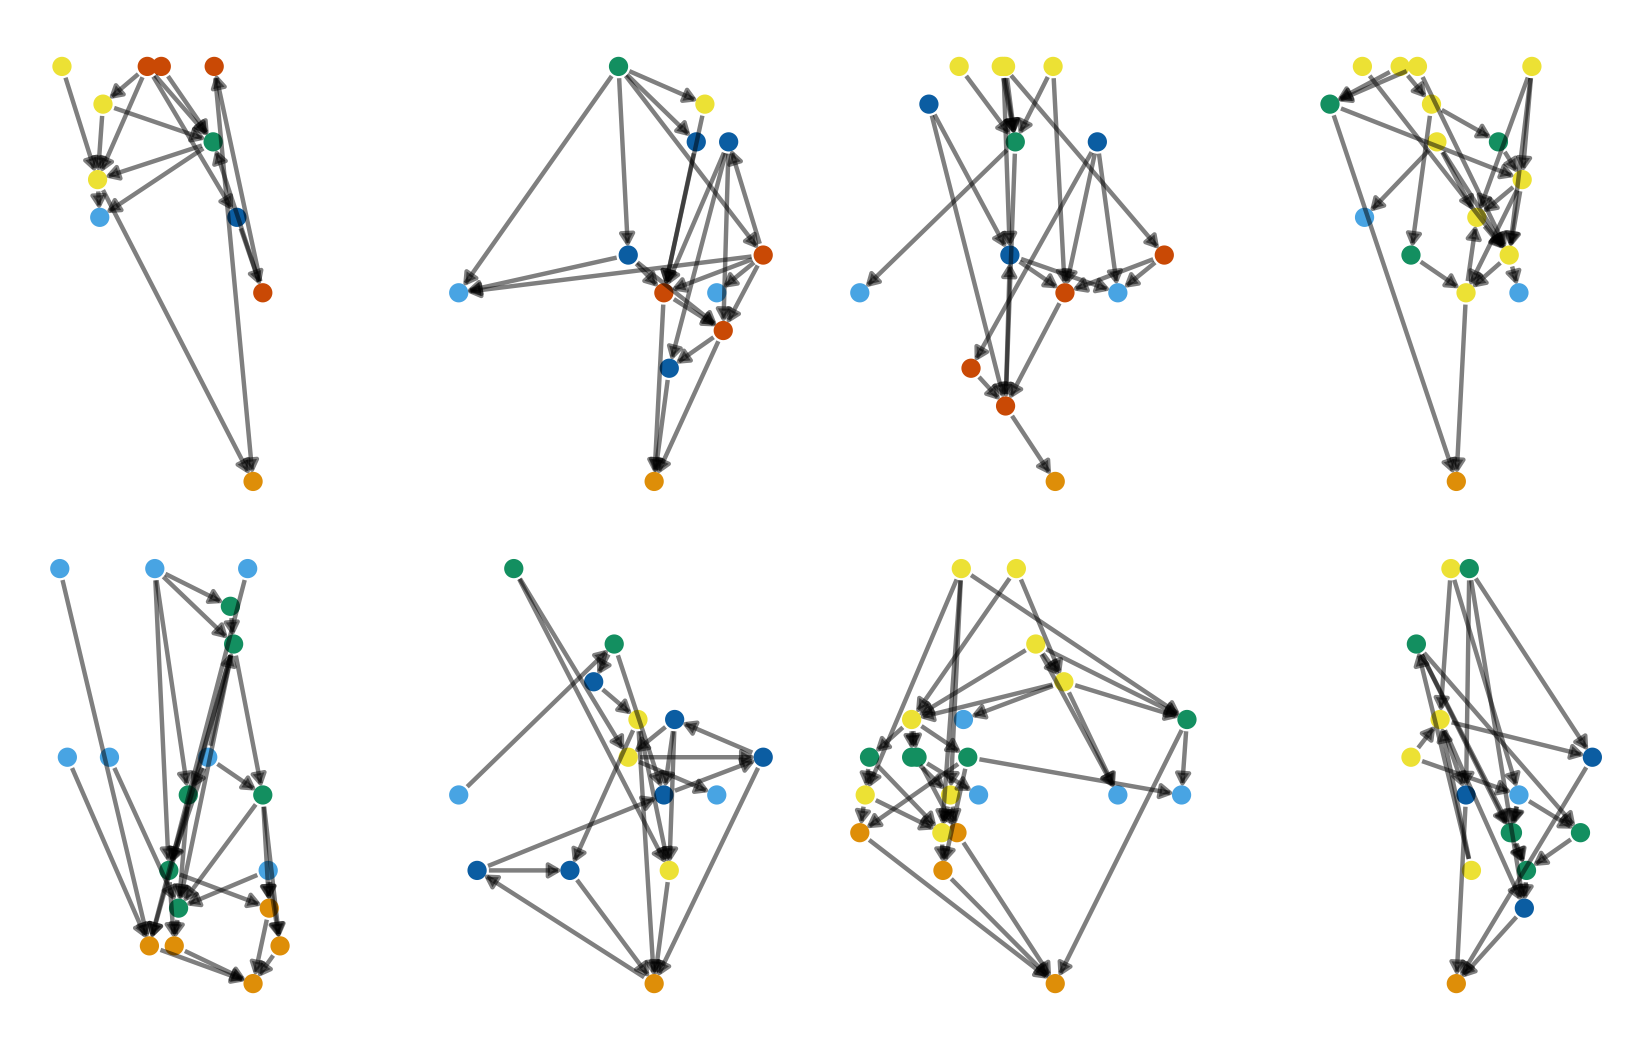
\includegraphics[keepaspectratio]{elicited-DAG-analysis_files/figure-pdf/unnamed-chunk-27-1.png}}

\begin{Shaded}
\begin{Highlighting}[]
\CommentTok{\# ggsave("dags\_All\_fine.svg", pAllFine, width = 18, height = 9)}
\end{Highlighting}
\end{Shaded}

\paragraph{Figure: Model graphs, all and
merged}\label{figure-model-graphs-all-and-merged}

\begin{Shaded}
\begin{Highlighting}[]
\FunctionTok{library}\NormalTok{(grid)}
\NormalTok{tag\_plot }\OtherTok{\textless{}{-}} \ControlFlowTok{function}\NormalTok{(p, tag, }\AttributeTok{x =} \DecValTok{0}\NormalTok{, }\AttributeTok{y =} \FloatTok{0.9}\NormalTok{, }\AttributeTok{fontsize =} \DecValTok{8}\NormalTok{) \{}
\NormalTok{  p }\SpecialCharTok{+} \FunctionTok{annotation\_custom}\NormalTok{(}
\NormalTok{    grid}\SpecialCharTok{::}\FunctionTok{textGrob}\NormalTok{(tag, }\AttributeTok{x =}\NormalTok{ x, }\AttributeTok{y =}\NormalTok{ y, }
                   \AttributeTok{hjust =} \DecValTok{0}\NormalTok{, }\AttributeTok{vjust =} \DecValTok{1}\NormalTok{, }\AttributeTok{gp =} \FunctionTok{gpar}\NormalTok{(}\AttributeTok{fontsize =}\NormalTok{ fontsize))}
\NormalTok{  )}
\NormalTok{\}}

\NormalTok{pAll3by3 }\OtherTok{\textless{}{-}} 
\NormalTok{    (}
        \FunctionTok{tag\_plot}\NormalTok{(p2peerHighlight,}\StringTok{"a"}\NormalTok{)}\SpecialCharTok{|} 
            \FunctionTok{tag\_plot}\NormalTok{(p8, }\StringTok{"b"}\NormalTok{) }\SpecialCharTok{|} 
            \FunctionTok{tag\_plot}\NormalTok{(p7KnHighlight, }\StringTok{"c"}\NormalTok{)) }\SpecialCharTok{/} 
\NormalTok{    (}
        \FunctionTok{tag\_plot}\NormalTok{(p4peerHighlight, }\StringTok{"d"}\NormalTok{) }\SpecialCharTok{|} 
            \FunctionTok{tag\_plot}\NormalTok{(p1, }\StringTok{"e"}\NormalTok{) }\SpecialCharTok{|} 
            \FunctionTok{tag\_plot}\NormalTok{(p5KnHighlight, }\StringTok{"f"}\NormalTok{)) }\SpecialCharTok{/} 
\NormalTok{    (}
        \FunctionTok{tag\_plot}\NormalTok{(p3peerHighlight, }\StringTok{"g"}\NormalTok{) }\SpecialCharTok{|} 
\NormalTok{            leg\_tall\_plot }\SpecialCharTok{|} 
            \FunctionTok{tag\_plot}\NormalTok{(p6KnHighlight, }\StringTok{"h"}\NormalTok{)) }
     

\NormalTok{pFineTogetherLabelled }\OtherTok{\textless{}{-}}\NormalTok{ pAll3by3 }\SpecialCharTok{/} \FunctionTok{tag\_plot}\NormalTok{(pMergedFineLabelled, }\StringTok{"i"}\NormalTok{) }\SpecialCharTok{+} \FunctionTok{plot\_layout}\NormalTok{(}\AttributeTok{heights =} \FunctionTok{c}\NormalTok{(}\DecValTok{1}\NormalTok{,}\DecValTok{1}\NormalTok{,}\DecValTok{1}\NormalTok{,}\DecValTok{3}\NormalTok{))}
\NormalTok{pFineTogether }\OtherTok{\textless{}{-}}\NormalTok{ pAll3by3 }\SpecialCharTok{/}\NormalTok{ pMergedFine }\SpecialCharTok{+} \FunctionTok{plot\_layout}\NormalTok{(}\AttributeTok{heights =} \FunctionTok{c}\NormalTok{(}\DecValTok{1}\NormalTok{,}\DecValTok{1}\NormalTok{,}\DecValTok{1}\NormalTok{,}\DecValTok{3}\NormalTok{))}
\NormalTok{pFineTogetherLabelled}
\end{Highlighting}
\end{Shaded}

\begin{verbatim}
Warning: ggrepel: 58 unlabeled data points (too many overlaps). Consider
increasing max.overlaps
\end{verbatim}

\pandocbounded{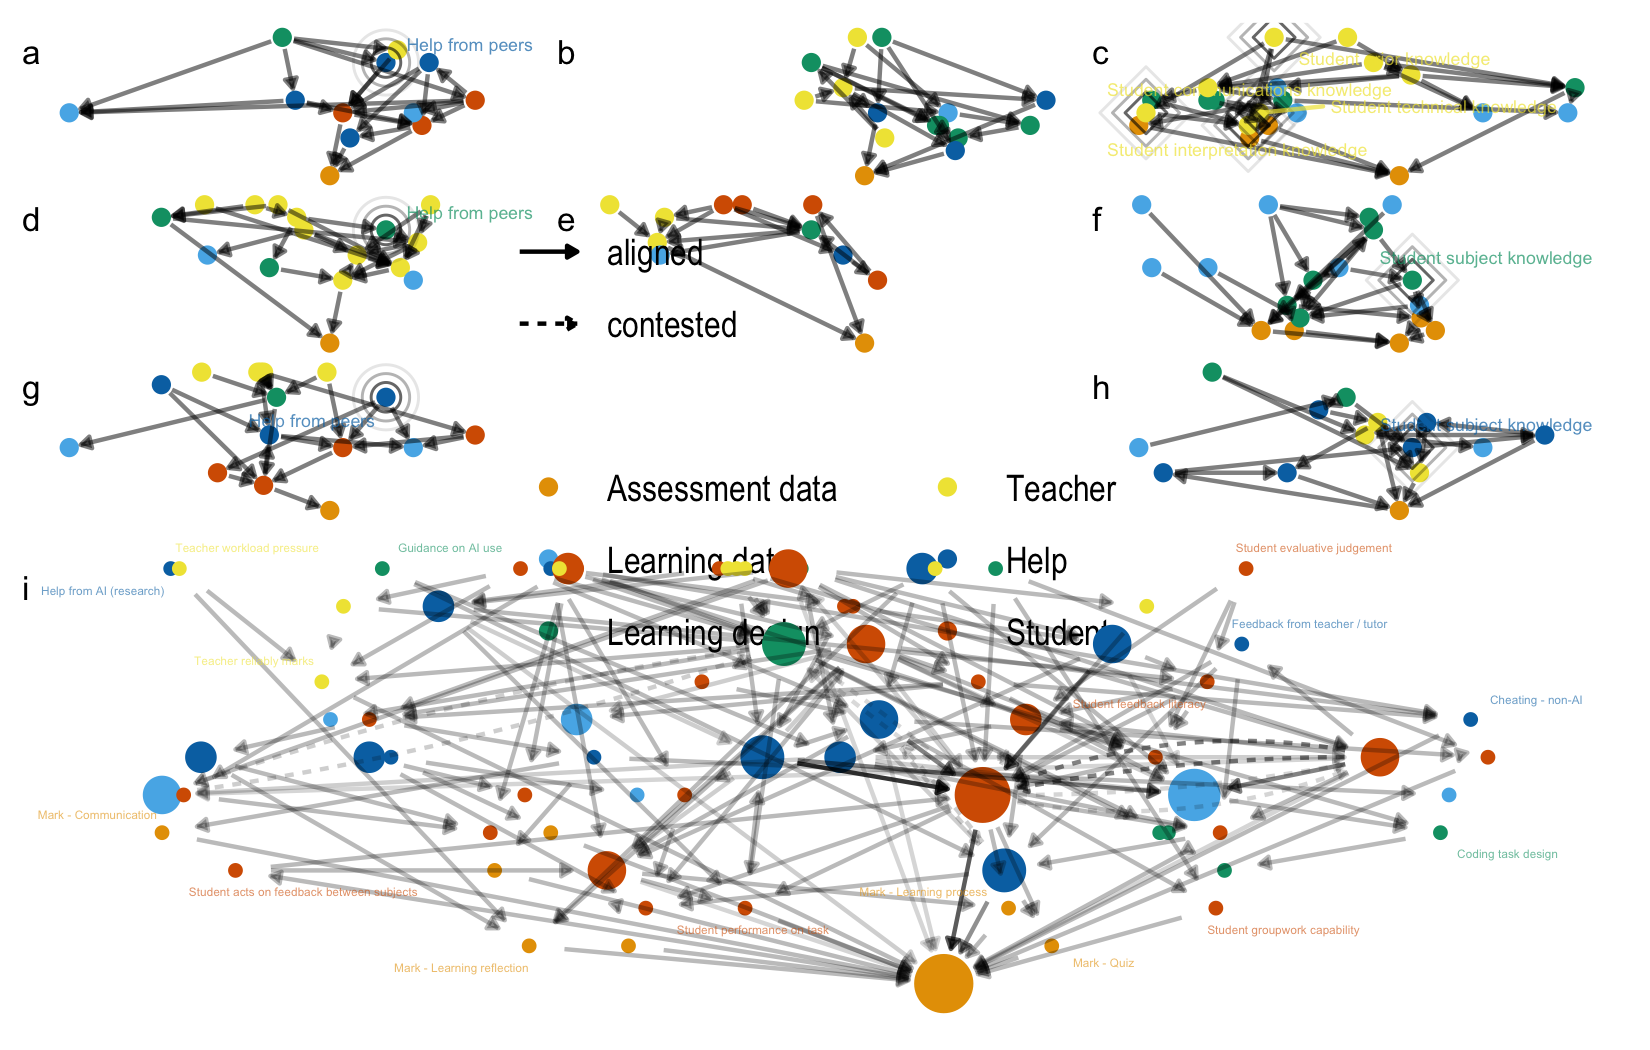
\includegraphics[keepaspectratio]{elicited-DAG-analysis_files/figure-pdf/unnamed-chunk-28-1.png}}

\begin{Shaded}
\begin{Highlighting}[]
\CommentTok{\# ggsave("dags\_fine\_all\_and\_merged.png", pFineTogether, width = 9, height = 10, dpi = 900)}
\CommentTok{\# ggsave("dags\_fine\_all\_and\_merged.svg", pFineTogether, width = 9, height = 10)}
\FunctionTok{ggsave}\NormalTok{(}\StringTok{"figures/FIG{-}{-}dags\_fine\_all\_and\_merged\_labelled.jpg"}\NormalTok{, pFineTogetherLabelled, }\AttributeTok{width =} \DecValTok{9}\NormalTok{, }\AttributeTok{height =} \DecValTok{10}\NormalTok{, }\AttributeTok{dpi =} \DecValTok{900}\NormalTok{)}
\end{Highlighting}
\end{Shaded}

\begin{verbatim}
Warning: ggrepel: 14 unlabeled data points (too many overlaps). Consider
increasing max.overlaps
\end{verbatim}

\begin{Shaded}
\begin{Highlighting}[]
\CommentTok{\# ggsave("dags\_fine\_all\_and\_merged\_labelled.svg", pFineTogetherLabelled, width = 9, height = 10)}

\FunctionTok{print}\NormalTok{(}\StringTok{"a, d, g are models S2, S3, S4; b, e are S8 and S1; c, f, h are S7, S5, S6. Closest models are therefore d and g (D{-}measure 0.105) and the furthest are e and 7 (D{-}measure 0.324)"}\NormalTok{)}
\end{Highlighting}
\end{Shaded}

\begin{verbatim}
[1] "a, d, g are models S2, S3, S4; b, e are S8 and S1; c, f, h are S7, S5, S6. Closest models are therefore d and g (D-measure 0.105) and the furthest are e and 7 (D-measure 0.324)"
\end{verbatim}

\paragraph{Common patterns - fine}\label{common-patterns---fine}

Most common three-node patterns.

\begin{Shaded}
\begin{Highlighting}[]
\NormalTok{merged\_all\_graph }\SpecialCharTok{|\textgreater{}} 
    \FunctionTok{activate}\NormalTok{(}\StringTok{"nodes"}\NormalTok{) }\SpecialCharTok{|\textgreater{}} 
    \FunctionTok{filter}\NormalTok{(node\_w }\SpecialCharTok{\textgreater{}} \DecValTok{3}\NormalTok{) }\SpecialCharTok{|\textgreater{}} 
    \FunctionTok{activate}\NormalTok{(}\StringTok{"edges"}\NormalTok{) }\SpecialCharTok{|\textgreater{}}
    \FunctionTok{filter}\NormalTok{(edge\_w }\SpecialCharTok{\textgreater{}} \DecValTok{1}\NormalTok{) }\SpecialCharTok{|\textgreater{}}
    \FunctionTok{g\_plot\_fine}\NormalTok{() }\SpecialCharTok{+}
    \FunctionTok{geom\_node\_text}\NormalTok{(}\FunctionTok{aes}\NormalTok{(}\AttributeTok{label =}\NormalTok{ nice\_name, }\AttributeTok{colour =}\NormalTok{ node\_type), }
                   \AttributeTok{alpha =}\NormalTok{ hl\_text\_alpha, }\AttributeTok{repel =} \ConstantTok{TRUE}\NormalTok{)}
\end{Highlighting}
\end{Shaded}

\pandocbounded{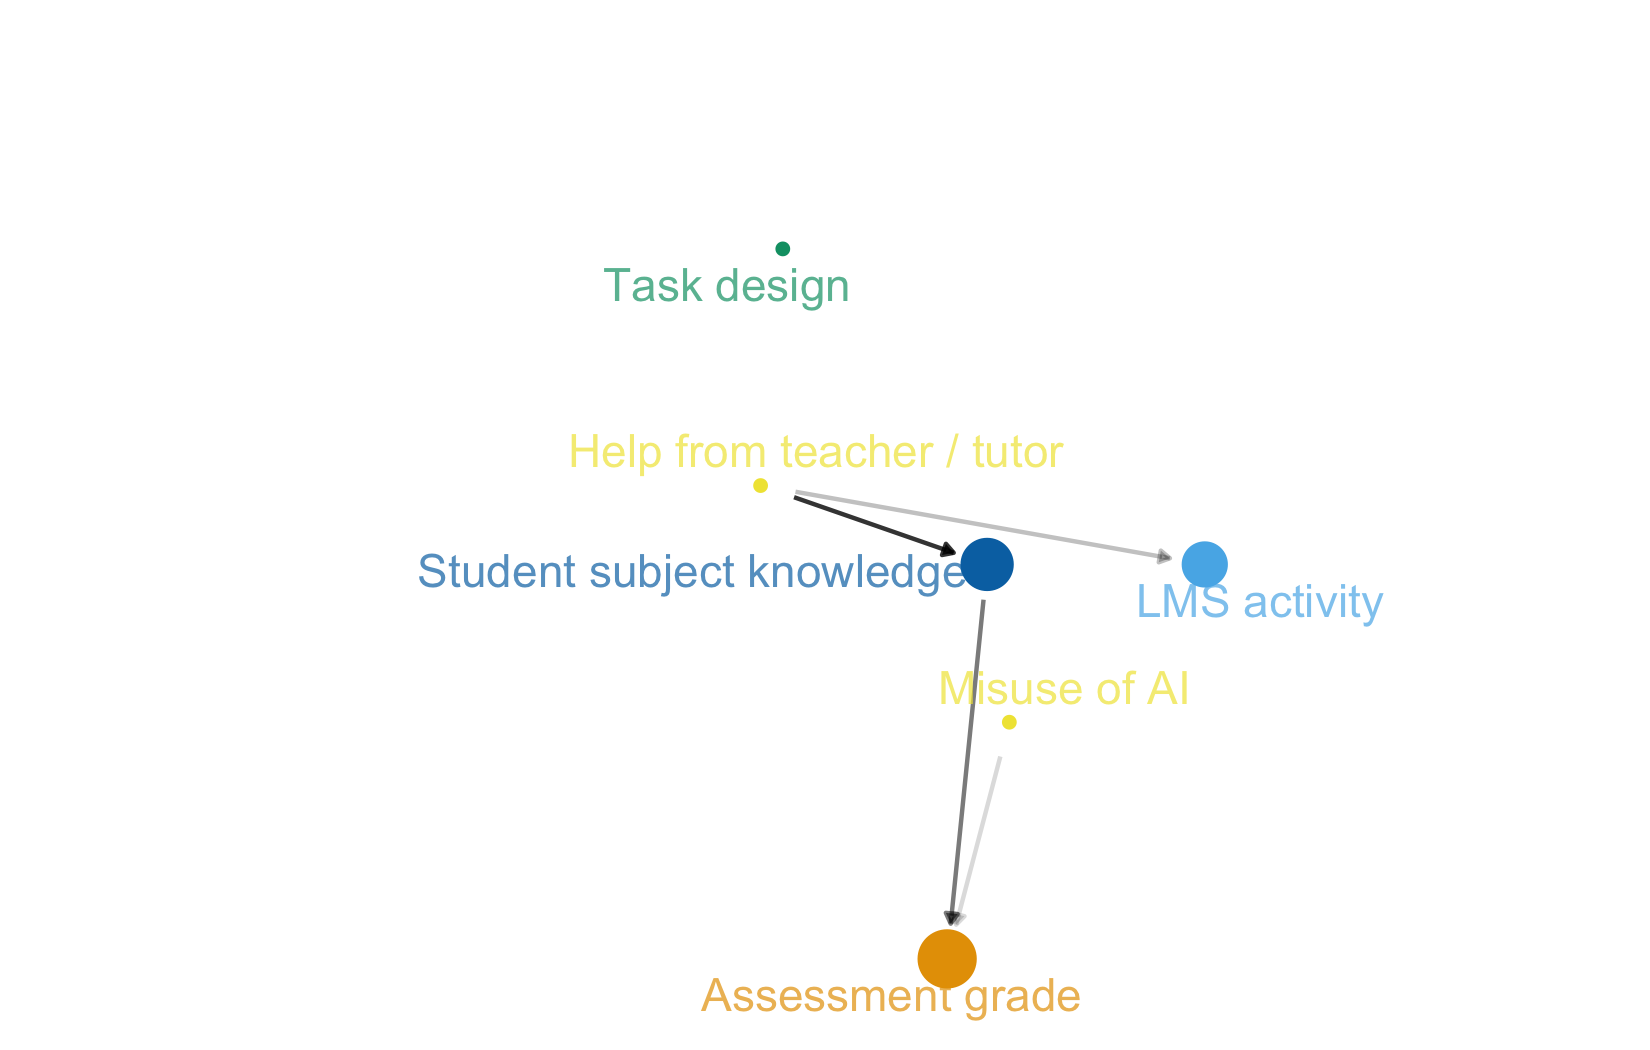
\includegraphics[keepaspectratio]{elicited-DAG-analysis_files/figure-pdf/unnamed-chunk-29-1.png}}

\subsubsection{Figure - all graphs, single
highlight}\label{figure---all-graphs-single-highlight}

\begin{Shaded}
\begin{Highlighting}[]
\NormalTok{plot\_highlighted\_fine\_graph }\OtherTok{\textless{}{-}} \ControlFlowTok{function}\NormalTok{(}\AttributeTok{model =} \DecValTok{1}\NormalTok{, }\AttributeTok{LEGEND\_POSITION =} \StringTok{"none"}\NormalTok{) \{}
\NormalTok{    MODEL }\OtherTok{\textless{}{-}} \FunctionTok{paste0}\NormalTok{(}\StringTok{"s"}\NormalTok{, model)}
\NormalTok{    nodes\_in\_graph }\OtherTok{\textless{}{-}}\NormalTok{ all\_nodes }\SpecialCharTok{|\textgreater{}} 
        \FunctionTok{filter}\NormalTok{(Model }\SpecialCharTok{==}\NormalTok{ MODEL) }\SpecialCharTok{|\textgreater{}} 
        \FunctionTok{pull}\NormalTok{(name)}
\NormalTok{    edges\_in\_graph }\OtherTok{\textless{}{-}}\NormalTok{ all\_edges }\SpecialCharTok{|\textgreater{}} 
        \FunctionTok{filter}\NormalTok{(Model }\SpecialCharTok{==}\NormalTok{ MODEL) }\SpecialCharTok{|\textgreater{}} 
        \FunctionTok{select}\NormalTok{(from, to)}
    
\NormalTok{    edges\_in\_graph\_indexed }\OtherTok{\textless{}{-}} 
\NormalTok{        edges\_in\_graph }\SpecialCharTok{|\textgreater{}} 
        \FunctionTok{mutate}\NormalTok{(}
            \AttributeTok{from =} \FunctionTok{match}\NormalTok{(from, merged\_all\_graph }\SpecialCharTok{\%N\textgreater{}\%} \FunctionTok{as\_tibble}\NormalTok{() }\SpecialCharTok{|\textgreater{}} \FunctionTok{pull}\NormalTok{(name)),}
            \AttributeTok{to =} \FunctionTok{match}\NormalTok{(to, merged\_all\_graph }\SpecialCharTok{\%N\textgreater{}\%} \FunctionTok{as\_tibble}\NormalTok{() }\SpecialCharTok{|\textgreater{}} \FunctionTok{pull}\NormalTok{(name))}
\NormalTok{        )}
    
\NormalTok{    g\_highlight }\OtherTok{\textless{}{-}}\NormalTok{ merged\_all\_graph }\SpecialCharTok{\%N\textgreater{}\%}
        \FunctionTok{mutate}\NormalTok{(}
            \AttributeTok{node\_highlight =} \FunctionTok{if\_else}\NormalTok{(}
\NormalTok{                name }\SpecialCharTok{\%in\%}\NormalTok{ nodes\_in\_graph, }\DecValTok{2}\NormalTok{, }\DecValTok{1}
\NormalTok{            )) }\SpecialCharTok{\%E\textgreater{}\%}
        \FunctionTok{left\_join}\NormalTok{(}
\NormalTok{            edges\_in\_graph\_indexed }\SpecialCharTok{|\textgreater{}} 
                \FunctionTok{mutate}\NormalTok{(}\AttributeTok{edge\_highlight =} \DecValTok{2}\NormalTok{)}
\NormalTok{        ) }\SpecialCharTok{|\textgreater{}} 
        \FunctionTok{mutate}\NormalTok{(}\AttributeTok{edge\_highlight =} \FunctionTok{replace\_na}\NormalTok{(edge\_highlight, }\DecValTok{1}\NormalTok{)) }\SpecialCharTok{|\textgreater{}} 
        \FunctionTok{create\_layout}\NormalTok{(}\StringTok{"sugiyama"}\NormalTok{)}
    
\NormalTok{    g\_highlight }\SpecialCharTok{|\textgreater{}}
        \FunctionTok{ggraph}\NormalTok{() }\SpecialCharTok{+}
        \FunctionTok{geom\_edge\_fan}\NormalTok{(}\FunctionTok{aes}\NormalTok{(}
            \CommentTok{\# edge\_linetype = factor(switched),}
            \AttributeTok{alpha =}\NormalTok{ edge\_highlight), }
            \AttributeTok{strength =} \FloatTok{0.2}\NormalTok{,}
            \AttributeTok{arrow =} \FunctionTok{arrow}\NormalTok{(}\AttributeTok{length =} \FunctionTok{unit}\NormalTok{(}\DecValTok{1}\NormalTok{, }\StringTok{\textquotesingle{}mm\textquotesingle{}}\NormalTok{),}
                          \AttributeTok{type =} \StringTok{"closed"}\NormalTok{),}
            \AttributeTok{start\_cap =} \FunctionTok{circle}\NormalTok{(}\DecValTok{3}\NormalTok{, }\StringTok{\textquotesingle{}mm\textquotesingle{}}\NormalTok{),}
            \AttributeTok{end\_cap =} \FunctionTok{circle}\NormalTok{(}\DecValTok{3}\NormalTok{, }\StringTok{\textquotesingle{}mm\textquotesingle{}}\NormalTok{)) }\SpecialCharTok{+}
        \FunctionTok{geom\_node\_label}\NormalTok{(}
            \FunctionTok{aes}\NormalTok{(}\AttributeTok{label =}\NormalTok{ nice\_name, }
                \AttributeTok{color =}\NormalTok{ node\_type,}
                \AttributeTok{size =}\NormalTok{ node\_w),}
            \AttributeTok{alpha =} \FloatTok{0.95}\NormalTok{,}
            \AttributeTok{data =}\NormalTok{ g\_highlight }\SpecialCharTok{|\textgreater{}} 
                \FunctionTok{filter}\NormalTok{(node\_highlight }\SpecialCharTok{==} \DecValTok{2}\NormalTok{),}
            \AttributeTok{repel =}\NormalTok{ T, }\AttributeTok{max.overlaps =} \DecValTok{30}\NormalTok{,}
            \AttributeTok{show.legend =} \ConstantTok{FALSE}\NormalTok{) }\SpecialCharTok{+}
        \FunctionTok{geom\_node\_point}\NormalTok{(}\FunctionTok{aes}\NormalTok{(}\AttributeTok{colour =}\NormalTok{ node\_type,}
                            \AttributeTok{size =}\NormalTok{ node\_w,}
                            \AttributeTok{alpha =}\NormalTok{ node\_highlight)) }\SpecialCharTok{+}
        \FunctionTok{scale\_size}\NormalTok{(}\AttributeTok{name =} \StringTok{"point{-}size"}\NormalTok{, }\AttributeTok{range =} \FunctionTok{c}\NormalTok{(}\DecValTok{2}\NormalTok{,}\DecValTok{5}\NormalTok{)) }\SpecialCharTok{+}
        \FunctionTok{scale\_color\_okabe\_ito}\NormalTok{(}\AttributeTok{order =} \FunctionTok{c}\NormalTok{(}\DecValTok{9}\NormalTok{, }\DecValTok{7}\NormalTok{,}\DecValTok{1}\NormalTok{, }\DecValTok{2}\NormalTok{,}\DecValTok{3}\NormalTok{, }\DecValTok{6}\NormalTok{, }\DecValTok{8}\NormalTok{,}\DecValTok{5}\NormalTok{, }\DecValTok{4}\NormalTok{)) }\SpecialCharTok{+}
        \CommentTok{\# scale\_color\_npg() +}
        \FunctionTok{theme\_graph}\NormalTok{() }\SpecialCharTok{+}
        \FunctionTok{scale\_edge\_alpha\_continuous}\NormalTok{(}\AttributeTok{range =} \FunctionTok{c}\NormalTok{(}\FloatTok{0.08}\NormalTok{,}\FloatTok{0.8}\NormalTok{)) }\SpecialCharTok{+}
        \FunctionTok{scale\_alpha\_continuous}\NormalTok{(}\AttributeTok{range =} \FunctionTok{c}\NormalTok{(}\FloatTok{0.1}\NormalTok{,}\FloatTok{1.0}\NormalTok{)) }\SpecialCharTok{+}
        \CommentTok{\# theme(legend.position = "none",}
        \CommentTok{\#       plot.margin = margin(t = 0, r = 0, b = 0, l = 0, unit = "pt")) +}
        \FunctionTok{theme}\NormalTok{(}\AttributeTok{legend.position =}\NormalTok{ LEGEND\_POSITION) }\SpecialCharTok{+}
        \FunctionTok{guides}\NormalTok{(}\AttributeTok{size =} \StringTok{"none"}\NormalTok{, }\AttributeTok{edge\_width =} \StringTok{"none"}\NormalTok{, }\AttributeTok{alpha =} \StringTok{"none"}\NormalTok{, }\AttributeTok{edge\_alpha =} \StringTok{"none"}\NormalTok{,}
               \AttributeTok{color =} \FunctionTok{guide\_legend}\NormalTok{(}\AttributeTok{ncol =} \DecValTok{1}\NormalTok{)) }\SpecialCharTok{+}
        \FunctionTok{theme}\NormalTok{(}\AttributeTok{legend.title =} \FunctionTok{element\_blank}\NormalTok{())}
\NormalTok{\}}

\FunctionTok{plot\_highlighted\_fine\_graph}\NormalTok{(}\DecValTok{4}\NormalTok{)}
\end{Highlighting}
\end{Shaded}

\begin{verbatim}
Joining with `by = join_by(from, to)`
\end{verbatim}

\pandocbounded{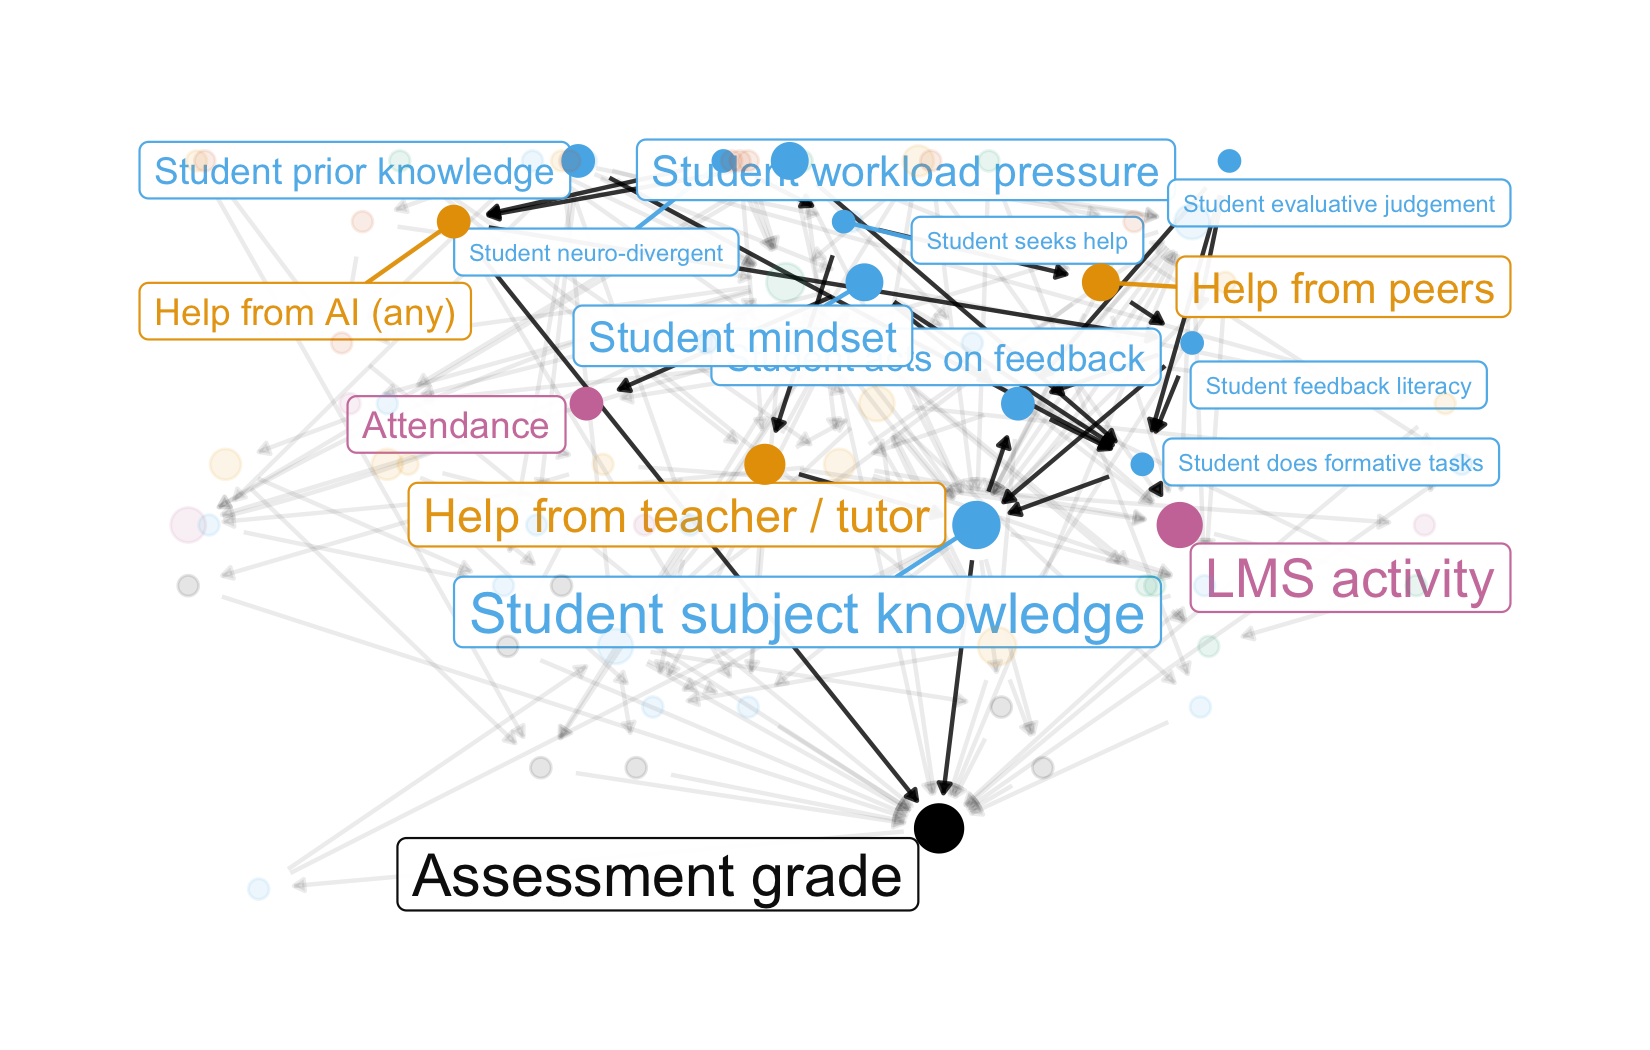
\includegraphics[keepaspectratio]{elicited-DAG-analysis_files/figure-pdf/unnamed-chunk-30-1.png}}

\begin{Shaded}
\begin{Highlighting}[]
\CommentTok{\# +}
\CommentTok{\#     xlim(x\_limits\_fine) +}
\CommentTok{\#     ylim(y\_limits\_fine)}



\NormalTok{plot\_highlighted\_coarse\_graph }\OtherTok{\textless{}{-}} \ControlFlowTok{function}\NormalTok{(}\AttributeTok{model =} \DecValTok{1}\NormalTok{, }\AttributeTok{LEGEND\_POSITION =} \StringTok{"none"}\NormalTok{) \{}
\NormalTok{    MODEL }\OtherTok{\textless{}{-}} \FunctionTok{paste0}\NormalTok{(}\StringTok{"s"}\NormalTok{, model)}
\NormalTok{    node\_groups\_in\_graph }\OtherTok{\textless{}{-}}\NormalTok{ all\_nodes }\SpecialCharTok{|\textgreater{}} 
        \FunctionTok{filter}\NormalTok{(Model }\SpecialCharTok{==}\NormalTok{ MODEL) }\SpecialCharTok{|\textgreater{}} 
        \FunctionTok{mutate}\NormalTok{(}\AttributeTok{name =} \FunctionTok{code\_node\_group}\NormalTok{(name)) }\SpecialCharTok{|\textgreater{}} 
        \FunctionTok{distinct}\NormalTok{(name) }\SpecialCharTok{|\textgreater{}} 
        \FunctionTok{pull}\NormalTok{(name) }
\NormalTok{    edges\_in\_coarse\_graph }\OtherTok{\textless{}{-}}\NormalTok{ all\_edges }\SpecialCharTok{|\textgreater{}} 
        \FunctionTok{filter}\NormalTok{(Model }\SpecialCharTok{==}\NormalTok{ MODEL) }\SpecialCharTok{|\textgreater{}} 
        \FunctionTok{select}\NormalTok{(from, to) }\SpecialCharTok{|\textgreater{}} 
        \FunctionTok{mutate}\NormalTok{(}\FunctionTok{across}\NormalTok{(from}\SpecialCharTok{:}\NormalTok{to, code\_node\_group))}
    
\NormalTok{    edges\_in\_graph\_indexed }\OtherTok{\textless{}{-}} 
\NormalTok{        edges\_in\_coarse\_graph }\SpecialCharTok{|\textgreater{}} 
        \FunctionTok{mutate}\NormalTok{(}
            \AttributeTok{from =} \FunctionTok{match}\NormalTok{(from, merged\_coarse\_models }\SpecialCharTok{\%N\textgreater{}\%} \FunctionTok{as\_tibble}\NormalTok{() }\SpecialCharTok{|\textgreater{}} \FunctionTok{pull}\NormalTok{(name)),}
            \AttributeTok{to =} \FunctionTok{match}\NormalTok{(to, merged\_coarse\_models }\SpecialCharTok{\%N\textgreater{}\%} \FunctionTok{as\_tibble}\NormalTok{() }\SpecialCharTok{|\textgreater{}} \FunctionTok{pull}\NormalTok{(name))}
\NormalTok{        )}
    
\NormalTok{    edge\_integers }\OtherTok{\textless{}{-}} 
\NormalTok{        edges\_in\_graph\_indexed }\SpecialCharTok{|\textgreater{}} 
        \FunctionTok{mutate}\NormalTok{(}\AttributeTok{p2p3 =}\NormalTok{ (}\DecValTok{2} \SpecialCharTok{**}\NormalTok{ from) }\SpecialCharTok{*}\NormalTok{ (}\DecValTok{3} \SpecialCharTok{**}\NormalTok{ to) ) }\SpecialCharTok{|\textgreater{}} 
        \FunctionTok{pull}\NormalTok{(p2p3)}
    
\NormalTok{    node\_types }\OtherTok{\textless{}{-}}\NormalTok{ merged\_all\_graph }\SpecialCharTok{\%N\textgreater{}\%}
        \FunctionTok{as\_tibble}\NormalTok{() }\SpecialCharTok{|\textgreater{}} 
        \FunctionTok{distinct}\NormalTok{(node\_group, node\_type) }
    
\NormalTok{    g\_highlight }\OtherTok{\textless{}{-}}\NormalTok{ merged\_coarse\_models }\SpecialCharTok{\%N\textgreater{}\%}
        \FunctionTok{inner\_join}\NormalTok{(node\_types }\SpecialCharTok{|\textgreater{}} \FunctionTok{rename}\NormalTok{(}\AttributeTok{name =}\NormalTok{ node\_group),}
                   \AttributeTok{by =} \StringTok{"name"}\NormalTok{) }\SpecialCharTok{|\textgreater{}}
        \FunctionTok{mutate}\NormalTok{(}
            \AttributeTok{node\_highlight =} \FunctionTok{if\_else}\NormalTok{(}
\NormalTok{                name }\SpecialCharTok{\%in\%}\NormalTok{ node\_groups\_in\_graph, }\DecValTok{2}\NormalTok{, }\DecValTok{1}
\NormalTok{            )) }\SpecialCharTok{\%E\textgreater{}\%}
        \FunctionTok{mutate}\NormalTok{(}\AttributeTok{edge\_highlight =} \FunctionTok{if\_else}\NormalTok{(}
\NormalTok{            ((}\DecValTok{2} \SpecialCharTok{**}\NormalTok{ from )}\SpecialCharTok{*}\NormalTok{(}\DecValTok{3} \SpecialCharTok{**}\NormalTok{ to)) }\SpecialCharTok{\%in\%}\NormalTok{ edge\_integers, }\DecValTok{2}\NormalTok{, }\DecValTok{1}
\NormalTok{        )) }\SpecialCharTok{|\textgreater{}} 
        \FunctionTok{create\_layout}\NormalTok{(}\StringTok{"sugiyama"}\NormalTok{)}
    
\NormalTok{    g\_highlight }\SpecialCharTok{|\textgreater{}}
        \FunctionTok{ggraph}\NormalTok{() }\SpecialCharTok{+}
        \FunctionTok{geom\_edge\_fan}\NormalTok{(}\FunctionTok{aes}\NormalTok{(}
            \CommentTok{\# edge\_linetype = factor(switched),}
            \AttributeTok{alpha =}\NormalTok{ edge\_highlight), }
            \AttributeTok{strength =} \FloatTok{0.2}\NormalTok{,}
            \AttributeTok{arrow =} \FunctionTok{arrow}\NormalTok{(}\AttributeTok{length =} \FunctionTok{unit}\NormalTok{(}\DecValTok{1}\NormalTok{, }\StringTok{\textquotesingle{}mm\textquotesingle{}}\NormalTok{),}
                          \AttributeTok{type =} \StringTok{"closed"}\NormalTok{),}
            \AttributeTok{start\_cap =} \FunctionTok{circle}\NormalTok{(}\DecValTok{3}\NormalTok{, }\StringTok{\textquotesingle{}mm\textquotesingle{}}\NormalTok{),}
            \AttributeTok{end\_cap =} \FunctionTok{circle}\NormalTok{(}\DecValTok{3}\NormalTok{, }\StringTok{\textquotesingle{}mm\textquotesingle{}}\NormalTok{)) }\SpecialCharTok{+}
        \FunctionTok{geom\_node\_label}\NormalTok{(}
            \FunctionTok{aes}\NormalTok{(}\AttributeTok{label =}\NormalTok{ nice\_name, }
                \AttributeTok{color =}\NormalTok{ node\_type,}
                \AttributeTok{size =}\NormalTok{ node\_w),}
            \AttributeTok{alpha =} \FloatTok{0.95}\NormalTok{,}
            \AttributeTok{data =}\NormalTok{ g\_highlight }\SpecialCharTok{|\textgreater{}} 
                \FunctionTok{filter}\NormalTok{(node\_highlight }\SpecialCharTok{==} \DecValTok{2}\NormalTok{),}
            \AttributeTok{repel =}\NormalTok{ T, }\AttributeTok{max.overlaps =} \DecValTok{30}\NormalTok{,}
            \AttributeTok{show.legend =} \ConstantTok{FALSE}\NormalTok{) }\SpecialCharTok{+}
        \FunctionTok{geom\_node\_point}\NormalTok{(}\FunctionTok{aes}\NormalTok{(}\AttributeTok{colour =}\NormalTok{ node\_type,}
                            \AttributeTok{size =}\NormalTok{ node\_w,}
                            \AttributeTok{alpha =}\NormalTok{ node\_highlight)) }\SpecialCharTok{+}
        \FunctionTok{scale\_size}\NormalTok{(}\AttributeTok{name =} \StringTok{"point{-}size"}\NormalTok{, }\AttributeTok{range =} \FunctionTok{c}\NormalTok{(}\DecValTok{2}\NormalTok{,}\DecValTok{5}\NormalTok{)) }\SpecialCharTok{+}
        \CommentTok{\# scale\_color\_npg() +}
        \FunctionTok{scale\_color\_okabe\_ito}\NormalTok{(}\AttributeTok{order =} \FunctionTok{c}\NormalTok{(}\DecValTok{9}\NormalTok{, }\DecValTok{7}\NormalTok{,}\DecValTok{1}\NormalTok{, }\DecValTok{2}\NormalTok{,}\DecValTok{3}\NormalTok{, }\DecValTok{6}\NormalTok{, }\DecValTok{8}\NormalTok{,}\DecValTok{5}\NormalTok{, }\DecValTok{4}\NormalTok{)) }\SpecialCharTok{+}
        \FunctionTok{theme\_graph}\NormalTok{() }\SpecialCharTok{+}
        \FunctionTok{scale\_edge\_alpha\_continuous}\NormalTok{(}\AttributeTok{range =} \FunctionTok{c}\NormalTok{(}\FloatTok{0.08}\NormalTok{,}\FloatTok{0.8}\NormalTok{)) }\SpecialCharTok{+}
        \FunctionTok{scale\_alpha\_continuous}\NormalTok{(}\AttributeTok{range =} \FunctionTok{c}\NormalTok{(}\FloatTok{0.1}\NormalTok{,}\FloatTok{1.0}\NormalTok{)) }\SpecialCharTok{+}
        \CommentTok{\# theme(legend.position = "none",}
        \CommentTok{\#       plot.margin = margin(t = 0, r = 0, b = 0, l = 0, unit = "pt")) +}
        \FunctionTok{theme}\NormalTok{(}\AttributeTok{legend.position =}\NormalTok{ LEGEND\_POSITION) }\SpecialCharTok{+}
        \FunctionTok{guides}\NormalTok{(}\AttributeTok{size =} \StringTok{"none"}\NormalTok{, }\AttributeTok{edge\_width =} \StringTok{"none"}\NormalTok{, }\AttributeTok{alpha =} \StringTok{"none"}\NormalTok{, }\AttributeTok{edge\_alpha =} \StringTok{"none"}\NormalTok{,}
               \AttributeTok{label =} \StringTok{"none"}\NormalTok{,}
               \AttributeTok{color =} \FunctionTok{guide\_legend}\NormalTok{(}\AttributeTok{ncol =} \DecValTok{1}\NormalTok{)) }\SpecialCharTok{+}
        \FunctionTok{theme}\NormalTok{(}\AttributeTok{legend.title =} \FunctionTok{element\_blank}\NormalTok{())}
\NormalTok{\}}

\CommentTok{\# Model used in paper}
\NormalTok{p\_merged\_highlighted\_fine }\OtherTok{\textless{}{-}} \FunctionTok{plot\_highlighted\_fine\_graph}\NormalTok{(}\DecValTok{5}\NormalTok{, }\AttributeTok{LEGEND\_POSITION =} \StringTok{"right"}\NormalTok{)}
\end{Highlighting}
\end{Shaded}

\begin{verbatim}
Joining with `by = join_by(from, to)`
\end{verbatim}

\begin{Shaded}
\begin{Highlighting}[]
\NormalTok{p\_merged\_highlighted\_coarse }\OtherTok{\textless{}{-}} \FunctionTok{plot\_highlighted\_coarse\_graph}\NormalTok{(}\DecValTok{5}\NormalTok{, }\AttributeTok{LEGEND\_POSITION =} \StringTok{"right"}\NormalTok{)}
\NormalTok{p\_merged\_highlighted\_fine }\SpecialCharTok{+} \FunctionTok{ggtitle}\NormalTok{(}\StringTok{"Model used in paper (5)"}\NormalTok{)}
\end{Highlighting}
\end{Shaded}

\pandocbounded{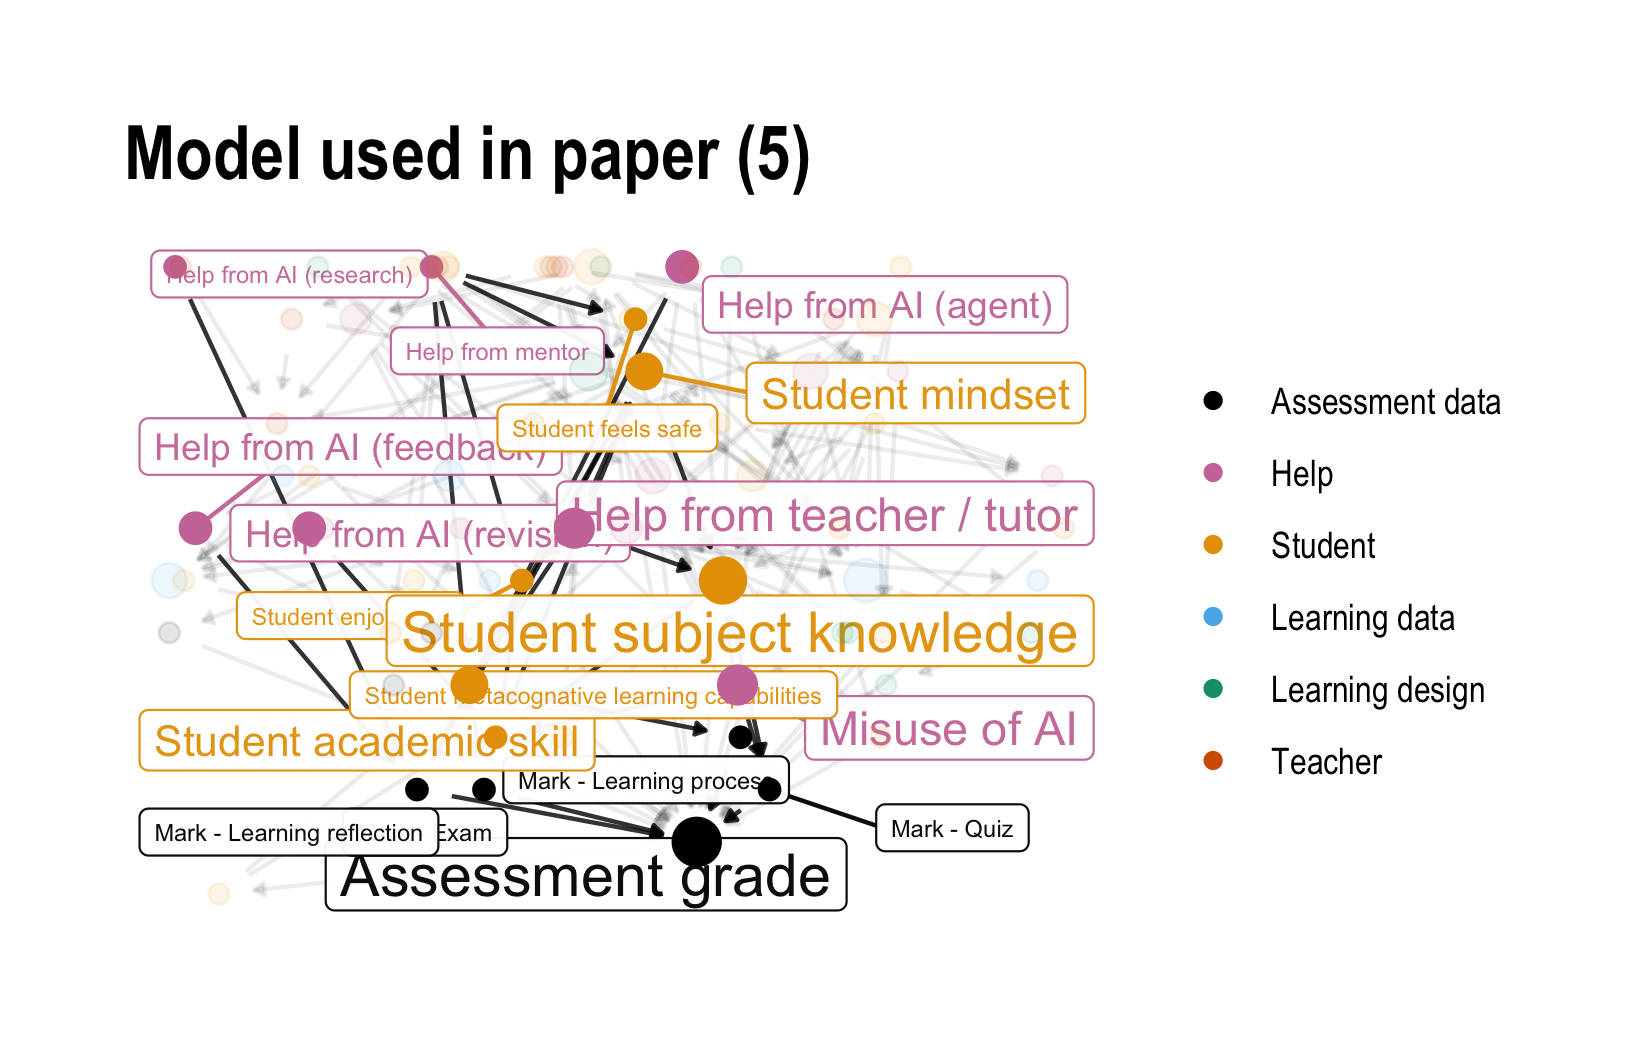
\includegraphics[keepaspectratio]{elicited-DAG-analysis_files/figure-pdf/unnamed-chunk-30-2.png}}

\begin{Shaded}
\begin{Highlighting}[]
\NormalTok{p\_merged\_highlighted\_coarse }
\end{Highlighting}
\end{Shaded}

\pandocbounded{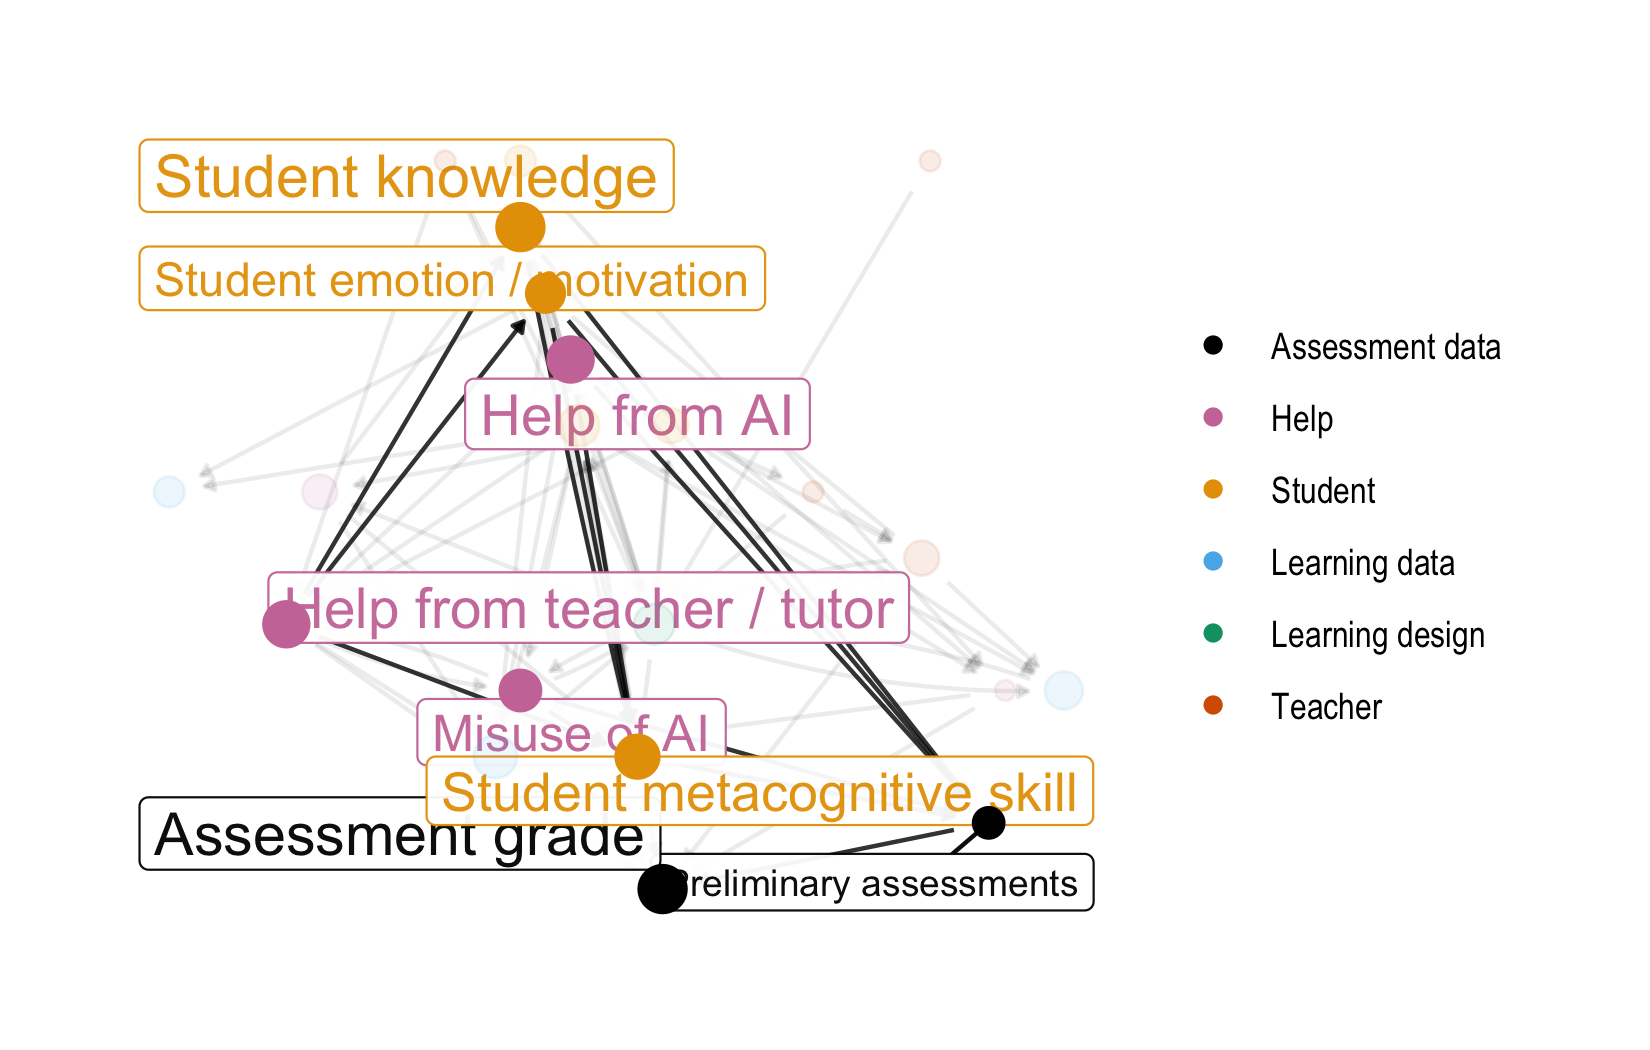
\includegraphics[keepaspectratio]{elicited-DAG-analysis_files/figure-pdf/unnamed-chunk-30-3.png}}

\begin{Shaded}
\begin{Highlighting}[]
\FunctionTok{ggsave}\NormalTok{(}\AttributeTok{plot =}\NormalTok{ p\_merged\_highlighted\_fine, }
       \AttributeTok{filename =} \StringTok{"figures/FIG{-}{-}merged{-}fine{-}with{-}1{-}highlighted.jpg"}\NormalTok{,}
       \AttributeTok{width =} \DecValTok{8}\NormalTok{, }\AttributeTok{height =} \DecValTok{5}\NormalTok{, }\AttributeTok{dpi =} \DecValTok{600}\NormalTok{)}

\FunctionTok{ggsave}\NormalTok{(}\AttributeTok{plot =}\NormalTok{ p\_merged\_highlighted\_coarse, }
       \AttributeTok{filename =} \StringTok{"figures/FIG{-}{-}merged{-}coarse{-}with{-}1{-}highlighted.jpg"}\NormalTok{,}
       \AttributeTok{width =} \DecValTok{8}\NormalTok{, }\AttributeTok{height =} \DecValTok{5}\NormalTok{, }\AttributeTok{dpi =} \DecValTok{600}\NormalTok{)}
\end{Highlighting}
\end{Shaded}

\begin{Shaded}
\begin{Highlighting}[]
\CommentTok{\# Generating all}
\NormalTok{p\_fine\_show\_and\_save }\OtherTok{\textless{}{-}} \ControlFlowTok{function}\NormalTok{(n)\{}
\NormalTok{    p\_temp }\OtherTok{\textless{}{-}} \FunctionTok{plot\_highlighted\_fine\_graph}\NormalTok{(n, }\AttributeTok{LEGEND\_POSITION =} \StringTok{"right"}\NormalTok{) }\SpecialCharTok{+} \FunctionTok{ggtitle}\NormalTok{(}\FunctionTok{paste0}\NormalTok{(}\StringTok{"Model "}\NormalTok{, n, }\StringTok{" highlighted"}\NormalTok{))}
    \FunctionTok{ggsave}\NormalTok{(}\AttributeTok{plot =}\NormalTok{ p\_temp, }
           \AttributeTok{filename =} \FunctionTok{paste0}\NormalTok{(}\StringTok{"figures/plt{-}{-}merged{-}fine{-}with{-}"}\NormalTok{, n, }\StringTok{"{-}highlighted.jpg"}\NormalTok{),}
           \AttributeTok{width =} \DecValTok{5}\NormalTok{, }\AttributeTok{height =} \DecValTok{3}\NormalTok{, }\AttributeTok{dpi =} \DecValTok{600}\NormalTok{)}
    \FunctionTok{return}\NormalTok{(p\_temp)}
\NormalTok{\}}
\NormalTok{p\_coarse\_show\_and\_save }\OtherTok{\textless{}{-}} \ControlFlowTok{function}\NormalTok{(n)\{}
\NormalTok{    p\_temp }\OtherTok{\textless{}{-}} \FunctionTok{plot\_highlighted\_coarse\_graph}\NormalTok{(n, }\AttributeTok{LEGEND\_POSITION =} \StringTok{"right"}\NormalTok{) }\SpecialCharTok{+} \FunctionTok{ggtitle}\NormalTok{(}\FunctionTok{paste0}\NormalTok{(}\StringTok{"Coarsened model "}\NormalTok{, n, }\StringTok{" highlighted"}\NormalTok{))}
    \FunctionTok{ggsave}\NormalTok{(}\AttributeTok{plot =}\NormalTok{ p\_temp, }
           \AttributeTok{filename =} \FunctionTok{paste0}\NormalTok{(}\StringTok{"figures/plt{-}{-}merged{-}coarse{-}with{-}"}\NormalTok{, n, }\StringTok{"{-}highlighted.jpg"}\NormalTok{),}
           \AttributeTok{width =} \DecValTok{5}\NormalTok{, }\AttributeTok{height =} \DecValTok{3}\NormalTok{, }\AttributeTok{dpi =} \DecValTok{600}\NormalTok{)}
    \FunctionTok{return}\NormalTok{(p\_temp)}
\NormalTok{\}}
\end{Highlighting}
\end{Shaded}

Highlighting all models in turn

\begin{Shaded}
\begin{Highlighting}[]
\FunctionTok{p\_fine\_show\_and\_save}\NormalTok{(}\DecValTok{1}\NormalTok{)}
\end{Highlighting}
\end{Shaded}

\begin{verbatim}
Joining with `by = join_by(from, to)`
\end{verbatim}

\pandocbounded{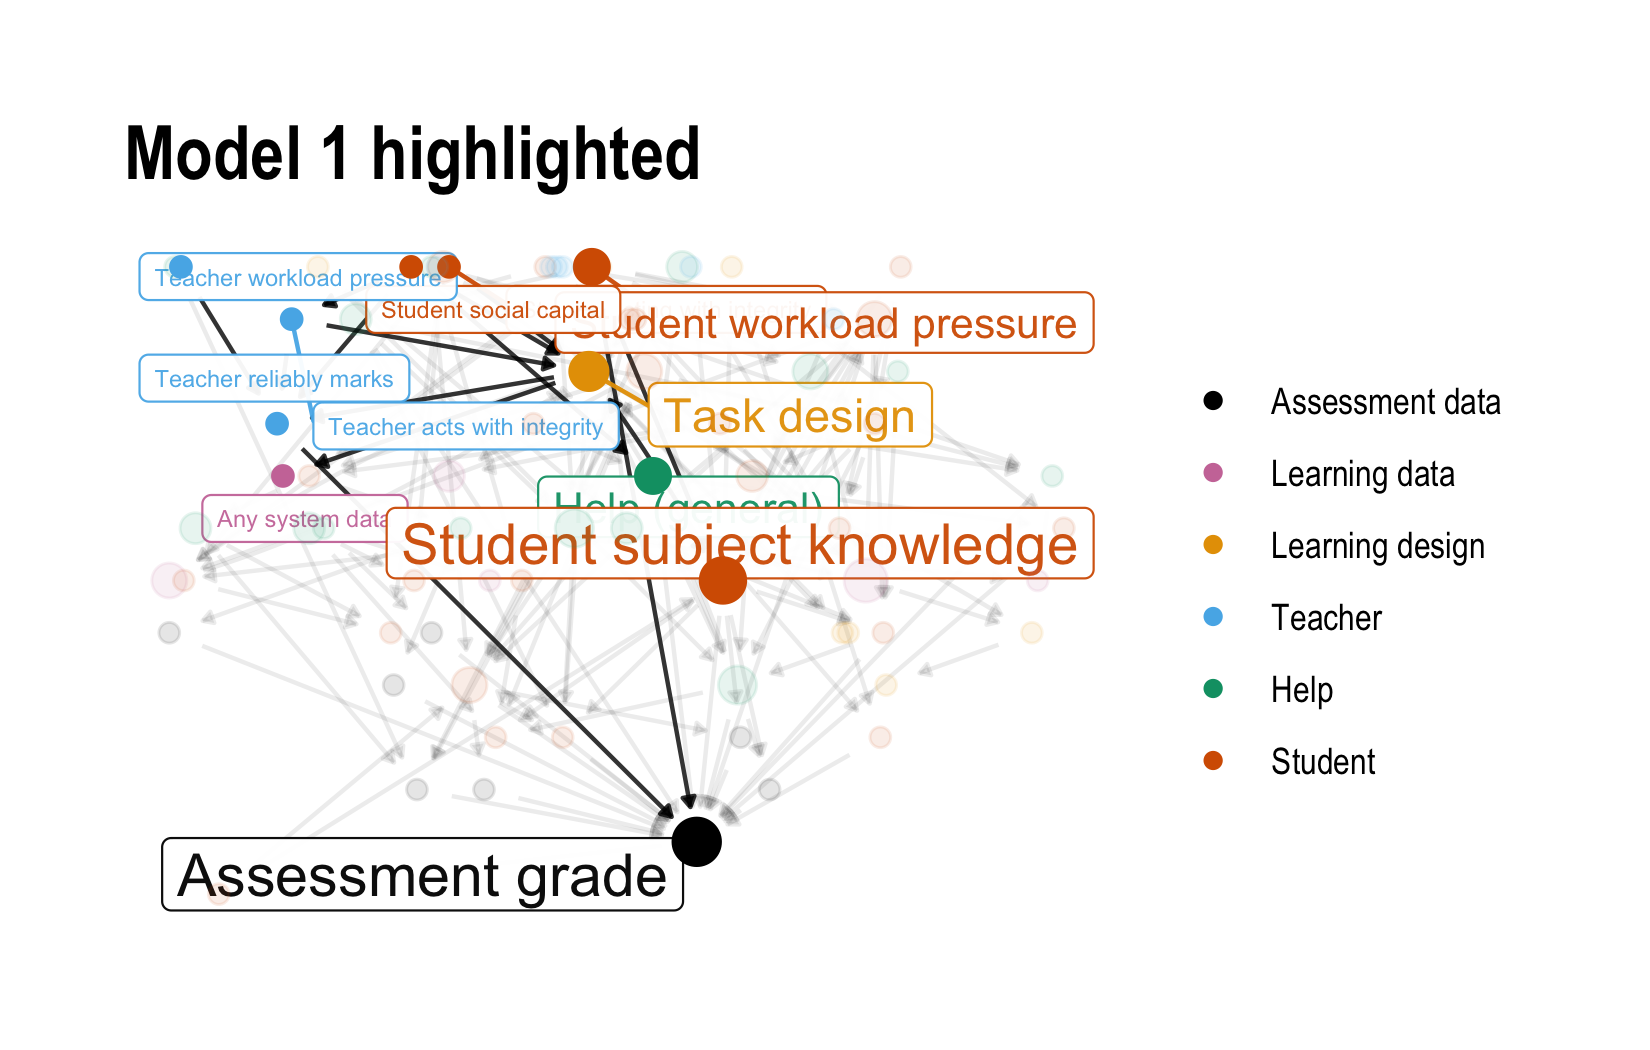
\includegraphics[keepaspectratio]{elicited-DAG-analysis_files/figure-pdf/unnamed-chunk-32-1.png}}

\begin{Shaded}
\begin{Highlighting}[]
\FunctionTok{p\_fine\_show\_and\_save}\NormalTok{(}\DecValTok{2}\NormalTok{)}
\end{Highlighting}
\end{Shaded}

\begin{verbatim}
Joining with `by = join_by(from, to)`
\end{verbatim}

\pandocbounded{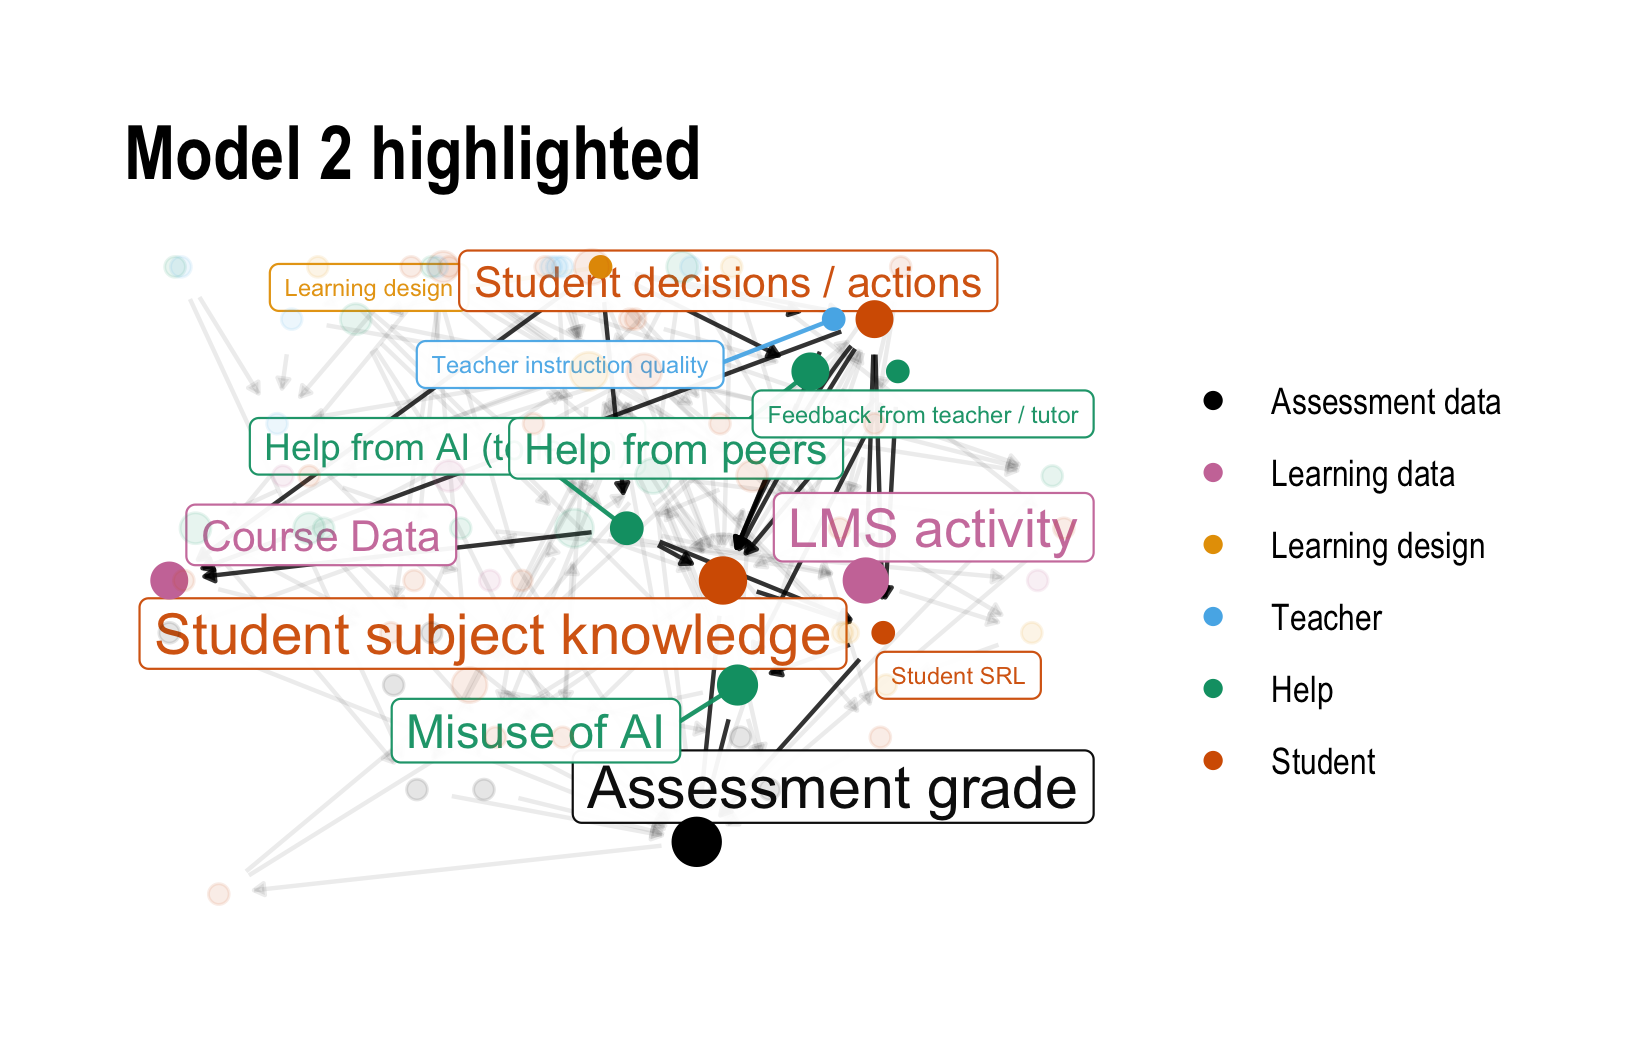
\includegraphics[keepaspectratio]{elicited-DAG-analysis_files/figure-pdf/unnamed-chunk-32-2.png}}

\begin{Shaded}
\begin{Highlighting}[]
\FunctionTok{p\_fine\_show\_and\_save}\NormalTok{(}\DecValTok{3}\NormalTok{)}
\end{Highlighting}
\end{Shaded}

\begin{verbatim}
Joining with `by = join_by(from, to)`
\end{verbatim}

\pandocbounded{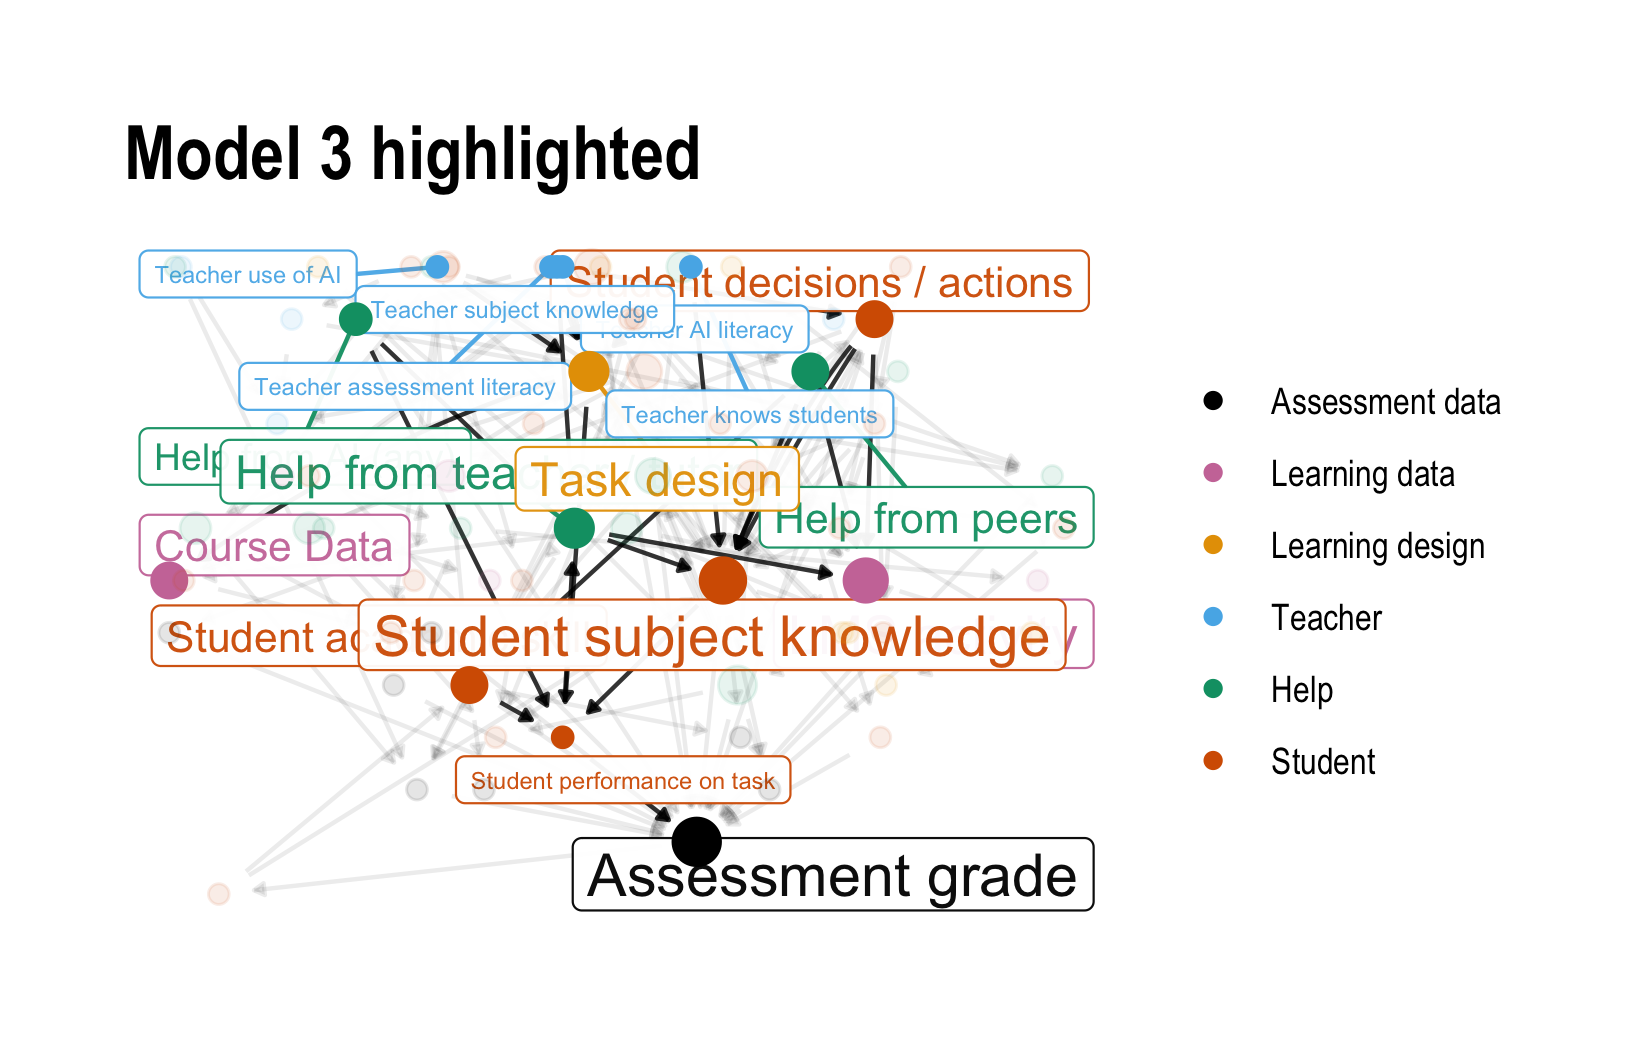
\includegraphics[keepaspectratio]{elicited-DAG-analysis_files/figure-pdf/unnamed-chunk-32-3.png}}

\begin{Shaded}
\begin{Highlighting}[]
\FunctionTok{p\_fine\_show\_and\_save}\NormalTok{(}\DecValTok{4}\NormalTok{)}
\end{Highlighting}
\end{Shaded}

\begin{verbatim}
Joining with `by = join_by(from, to)`
\end{verbatim}

\pandocbounded{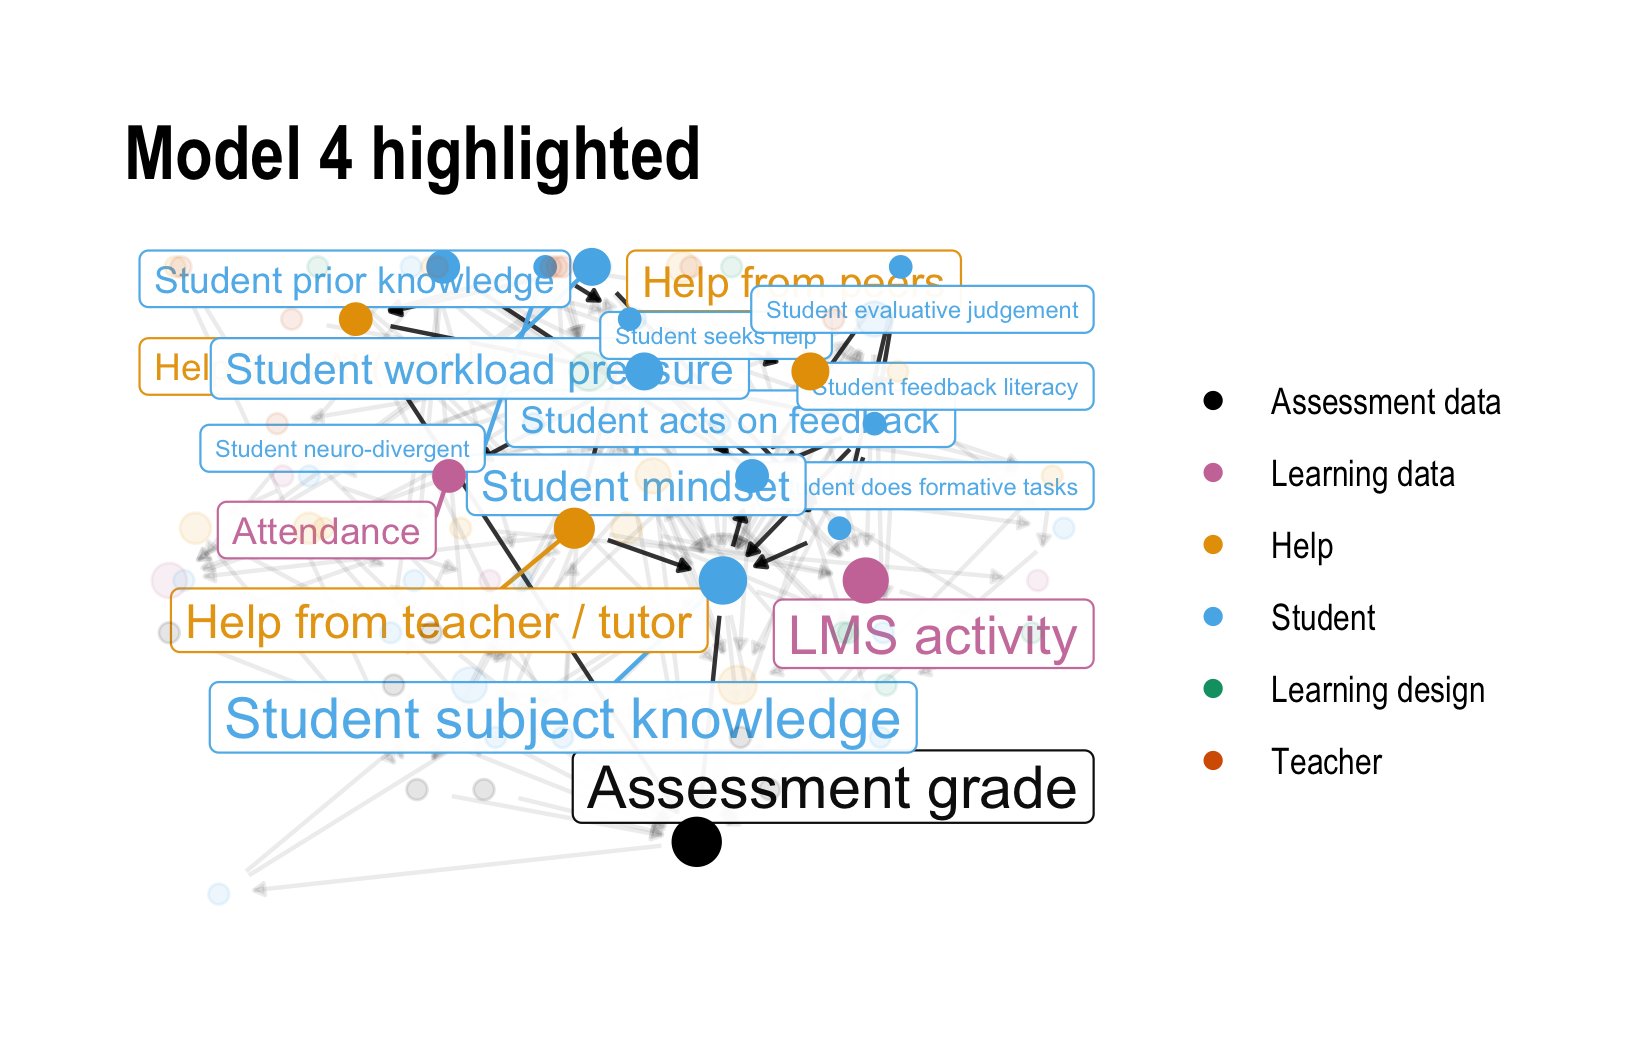
\includegraphics[keepaspectratio]{elicited-DAG-analysis_files/figure-pdf/unnamed-chunk-32-4.png}}

\begin{Shaded}
\begin{Highlighting}[]
\FunctionTok{p\_fine\_show\_and\_save}\NormalTok{(}\DecValTok{5}\NormalTok{)}
\end{Highlighting}
\end{Shaded}

\begin{verbatim}
Joining with `by = join_by(from, to)`
\end{verbatim}

\pandocbounded{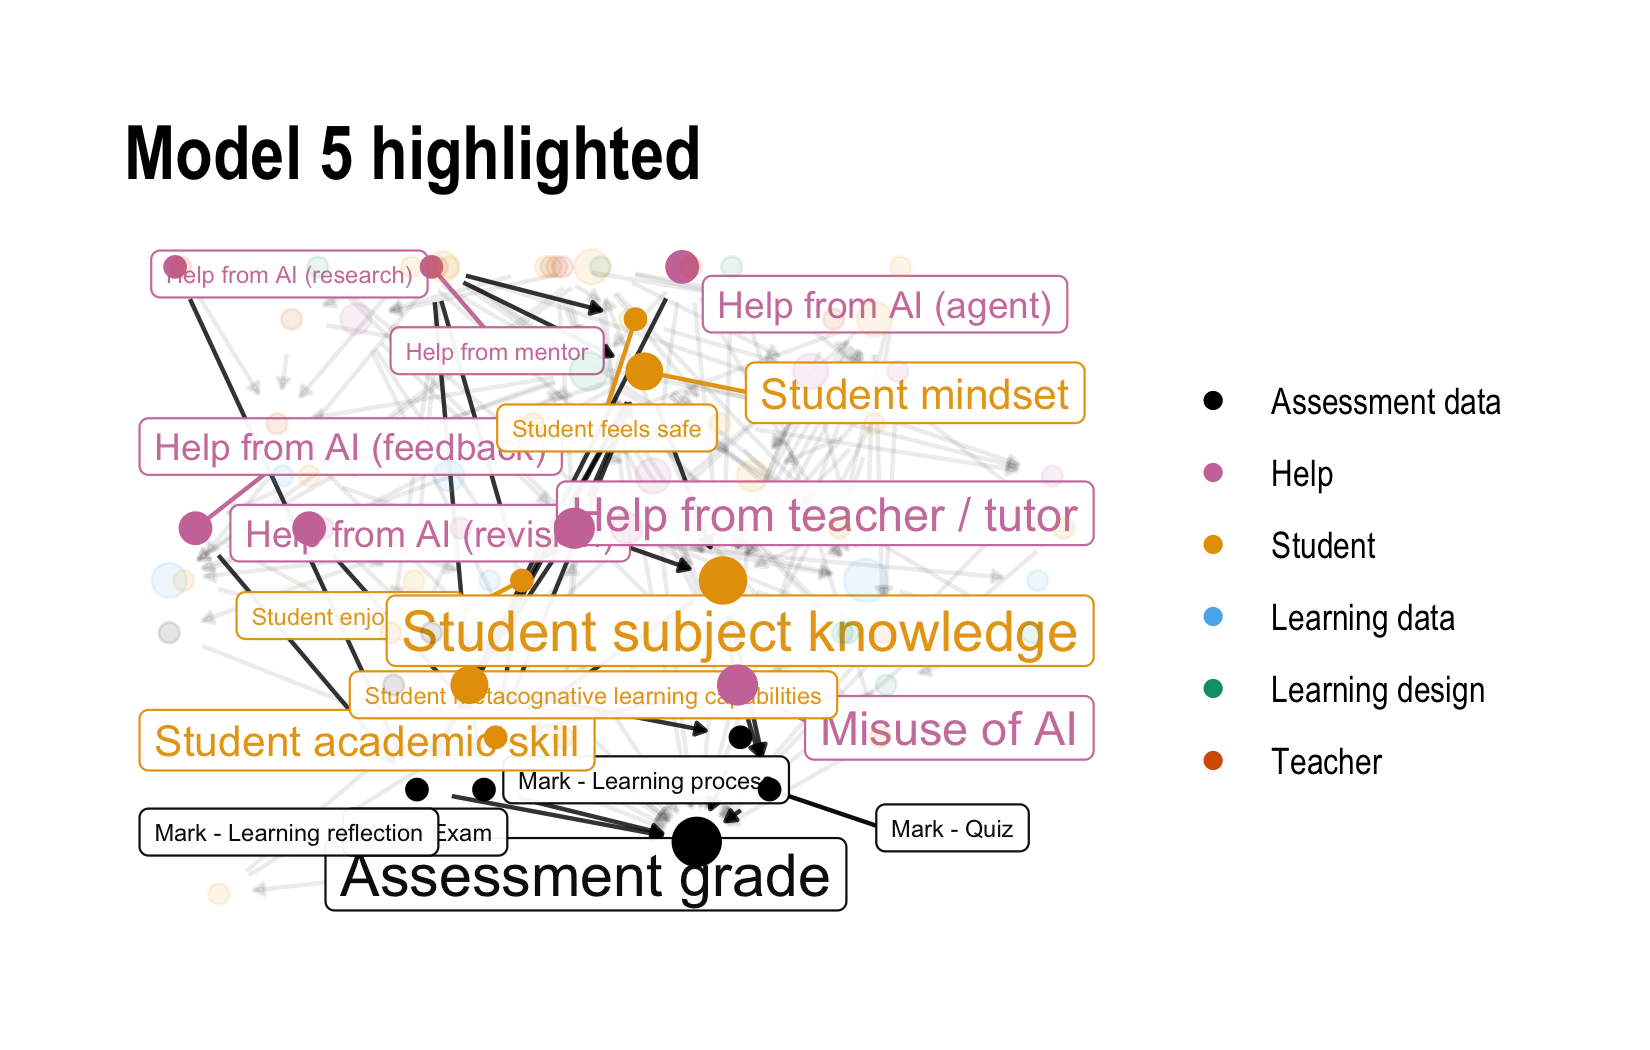
\includegraphics[keepaspectratio]{elicited-DAG-analysis_files/figure-pdf/unnamed-chunk-32-5.png}}

\begin{Shaded}
\begin{Highlighting}[]
\FunctionTok{p\_fine\_show\_and\_save}\NormalTok{(}\DecValTok{6}\NormalTok{)}
\end{Highlighting}
\end{Shaded}

\begin{verbatim}
Joining with `by = join_by(from, to)`
\end{verbatim}

\pandocbounded{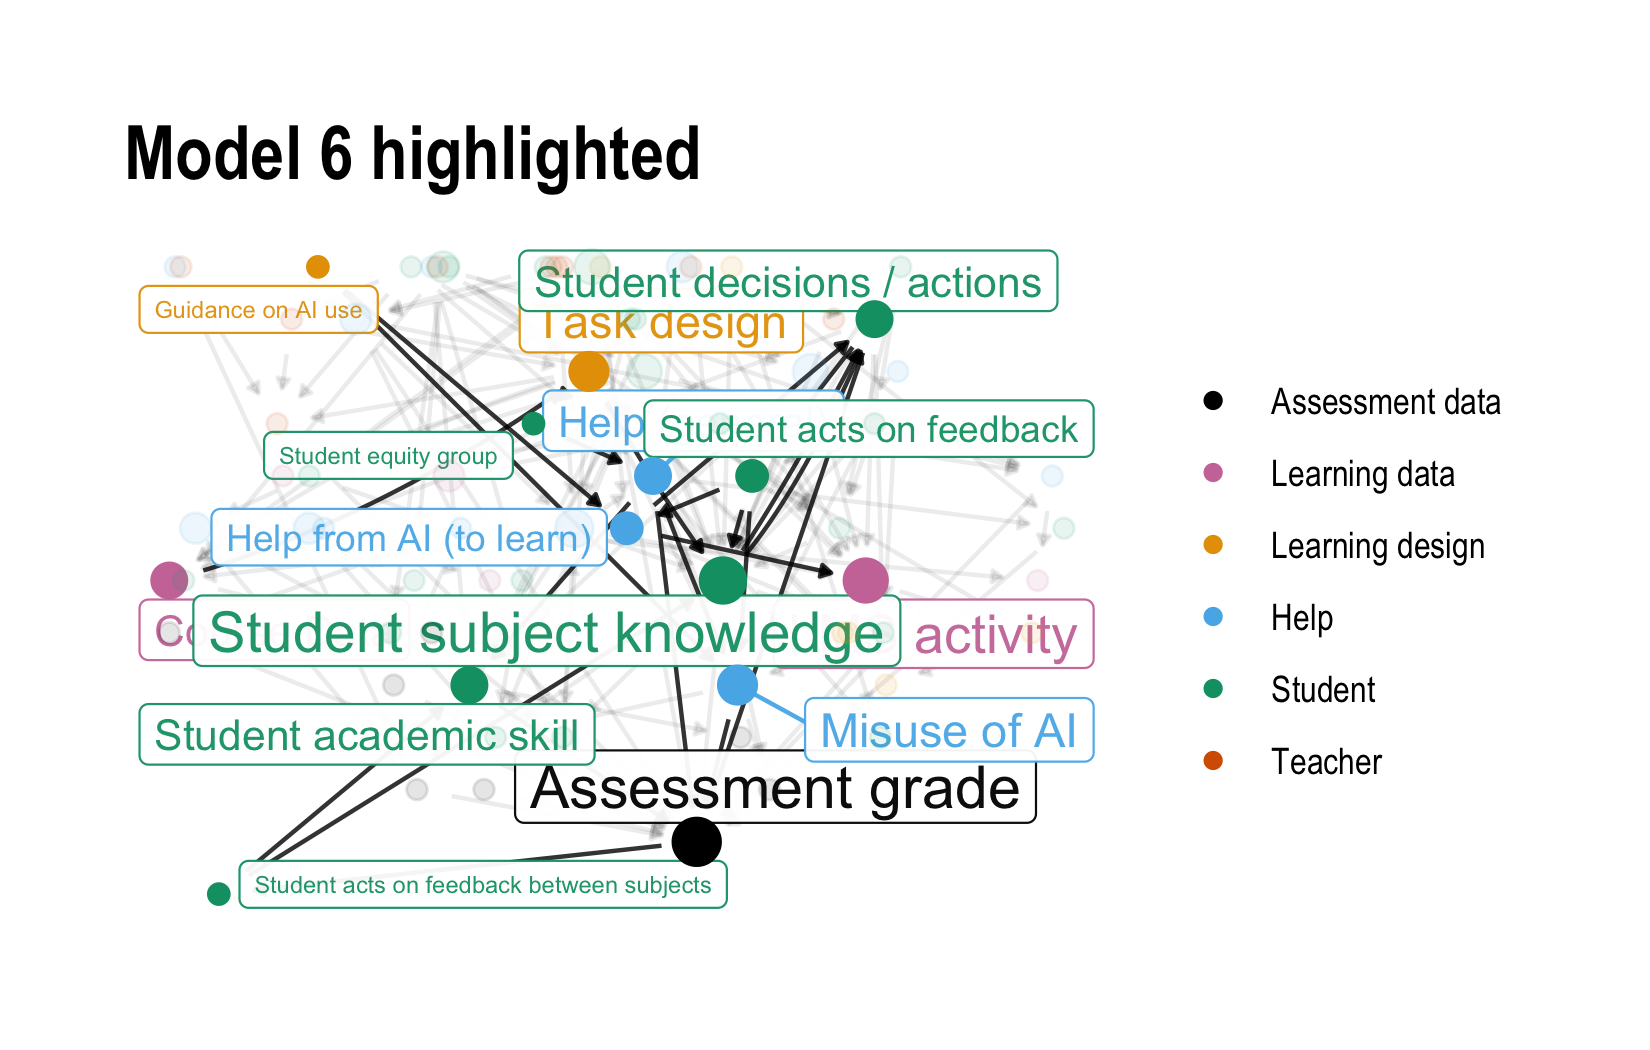
\includegraphics[keepaspectratio]{elicited-DAG-analysis_files/figure-pdf/unnamed-chunk-32-6.png}}

\begin{Shaded}
\begin{Highlighting}[]
\FunctionTok{p\_fine\_show\_and\_save}\NormalTok{(}\DecValTok{7}\NormalTok{)}
\end{Highlighting}
\end{Shaded}

\begin{verbatim}
Joining with `by = join_by(from, to)`
\end{verbatim}

\pandocbounded{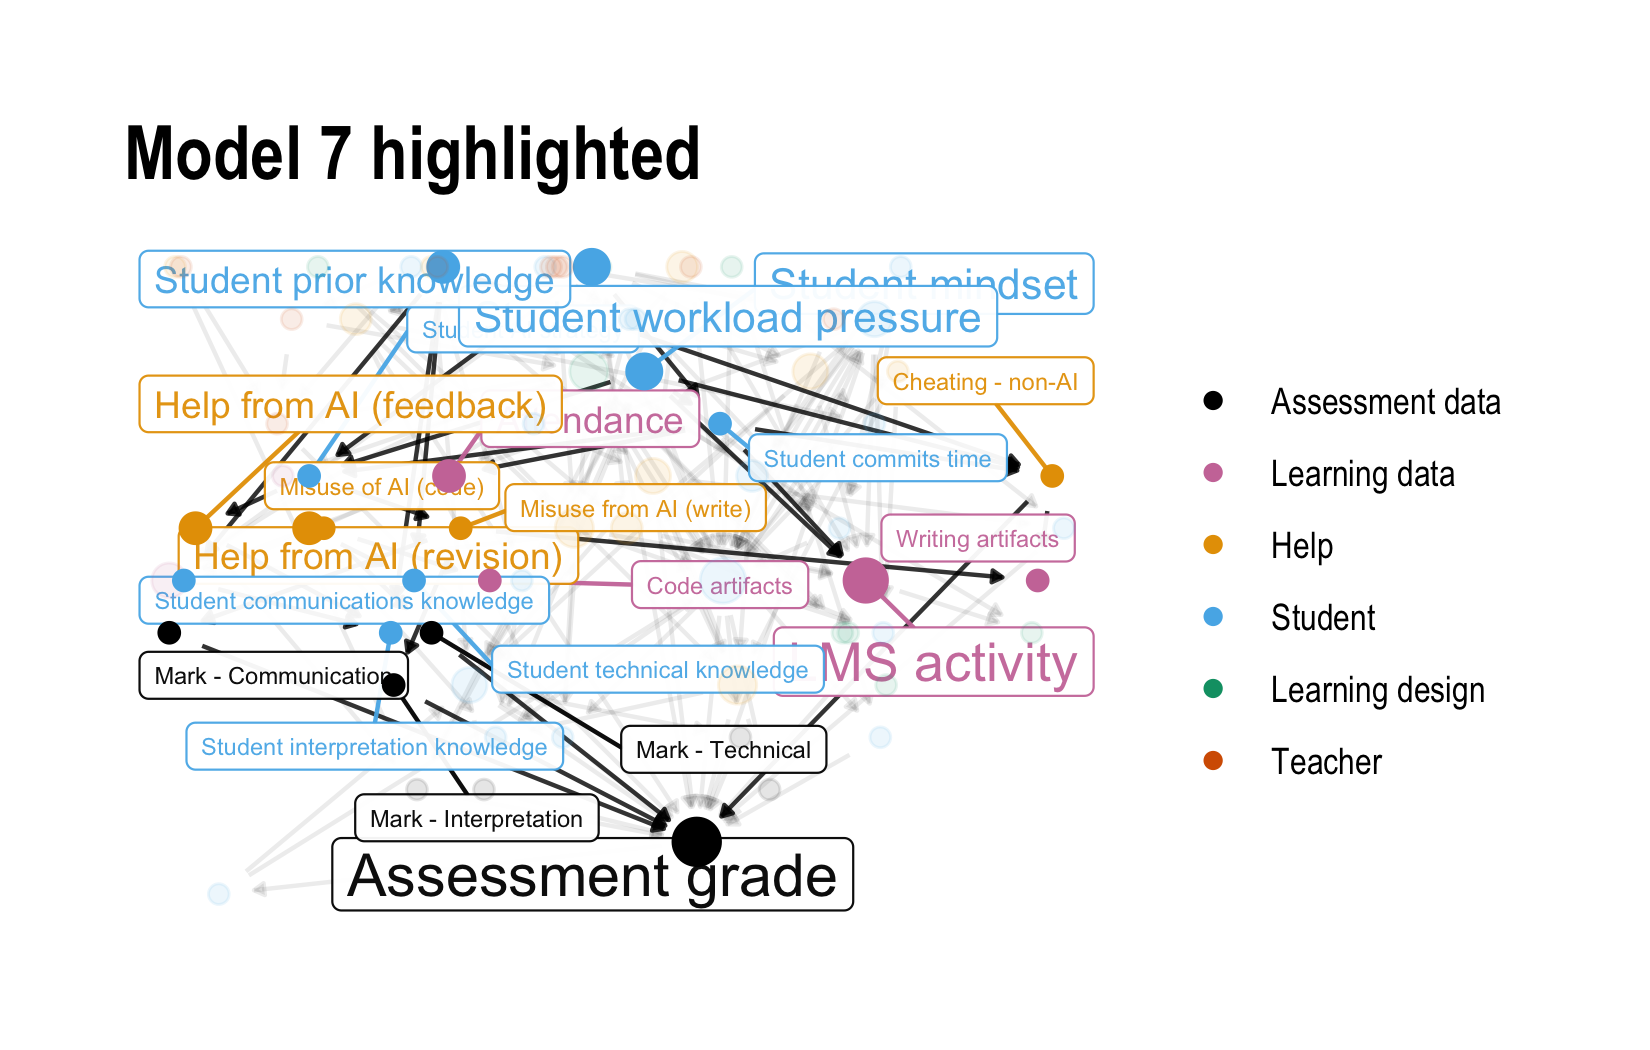
\includegraphics[keepaspectratio]{elicited-DAG-analysis_files/figure-pdf/unnamed-chunk-32-7.png}}

\begin{Shaded}
\begin{Highlighting}[]
\FunctionTok{p\_fine\_show\_and\_save}\NormalTok{(}\DecValTok{8}\NormalTok{)}
\end{Highlighting}
\end{Shaded}

\begin{verbatim}
Joining with `by = join_by(from, to)`
\end{verbatim}

\pandocbounded{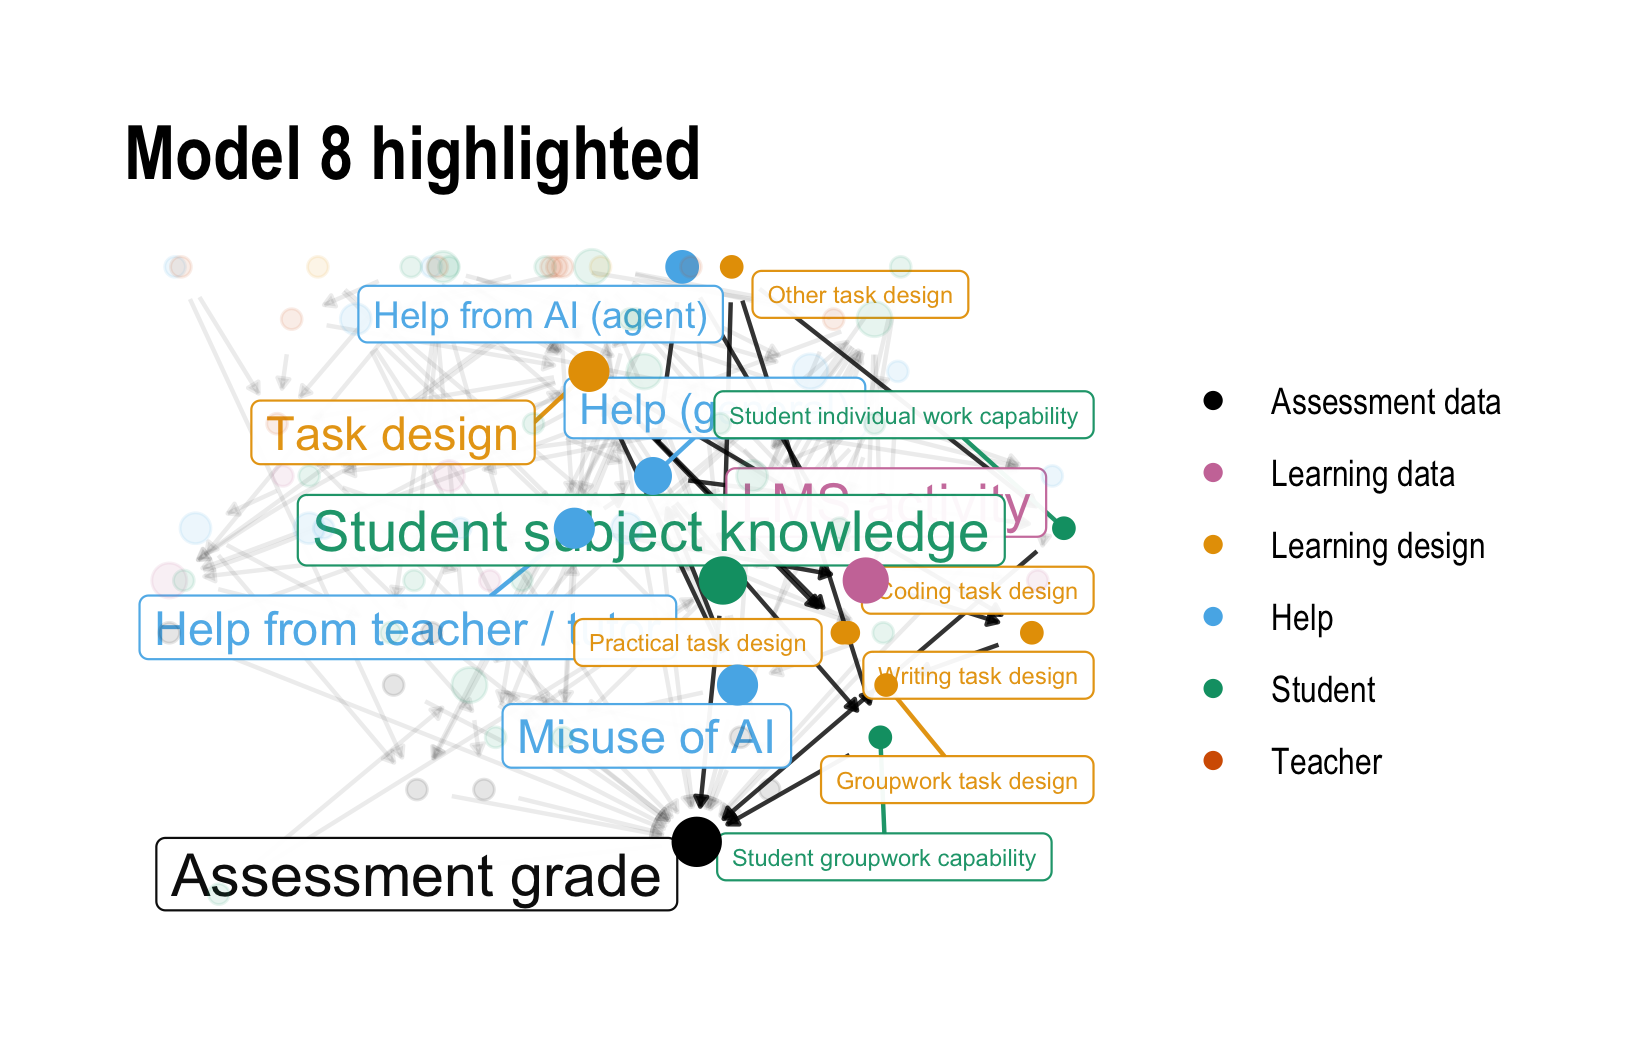
\includegraphics[keepaspectratio]{elicited-DAG-analysis_files/figure-pdf/unnamed-chunk-32-8.png}}

Highlighting all coarsened models in turn

\begin{Shaded}
\begin{Highlighting}[]
\FunctionTok{p\_coarse\_show\_and\_save}\NormalTok{(}\DecValTok{1}\NormalTok{)}
\end{Highlighting}
\end{Shaded}

\pandocbounded{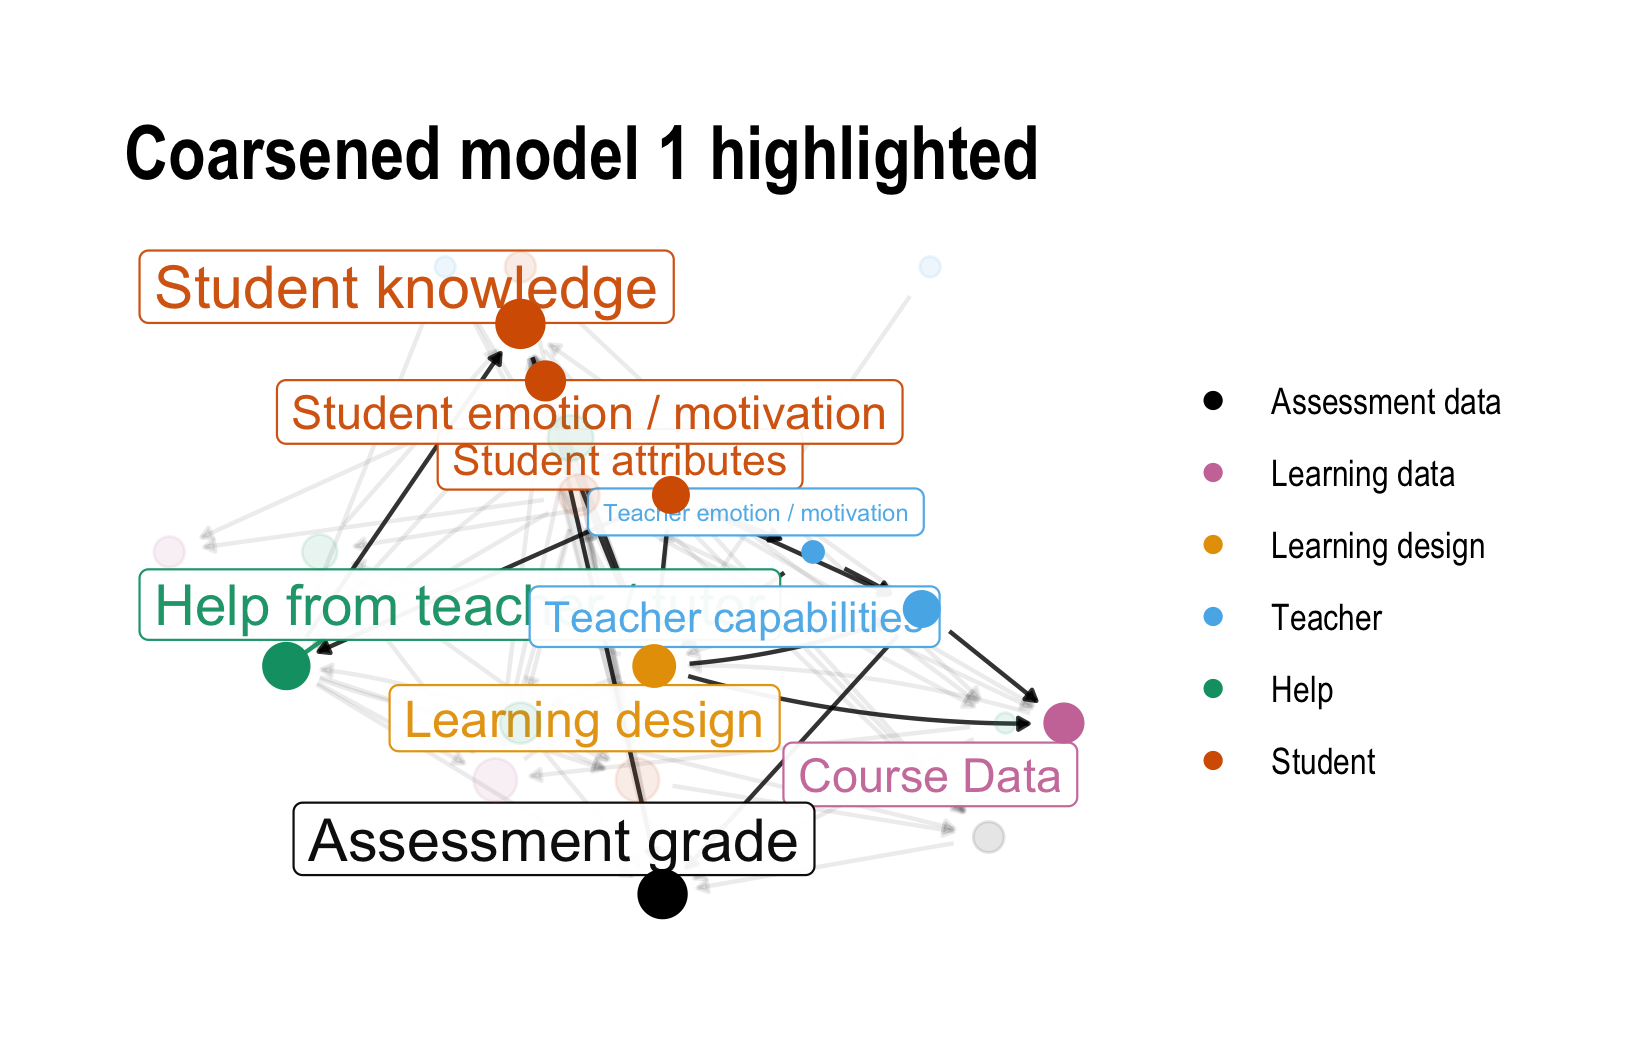
\includegraphics[keepaspectratio]{elicited-DAG-analysis_files/figure-pdf/unnamed-chunk-33-1.png}}

\begin{Shaded}
\begin{Highlighting}[]
\FunctionTok{p\_coarse\_show\_and\_save}\NormalTok{(}\DecValTok{2}\NormalTok{)}
\end{Highlighting}
\end{Shaded}

\pandocbounded{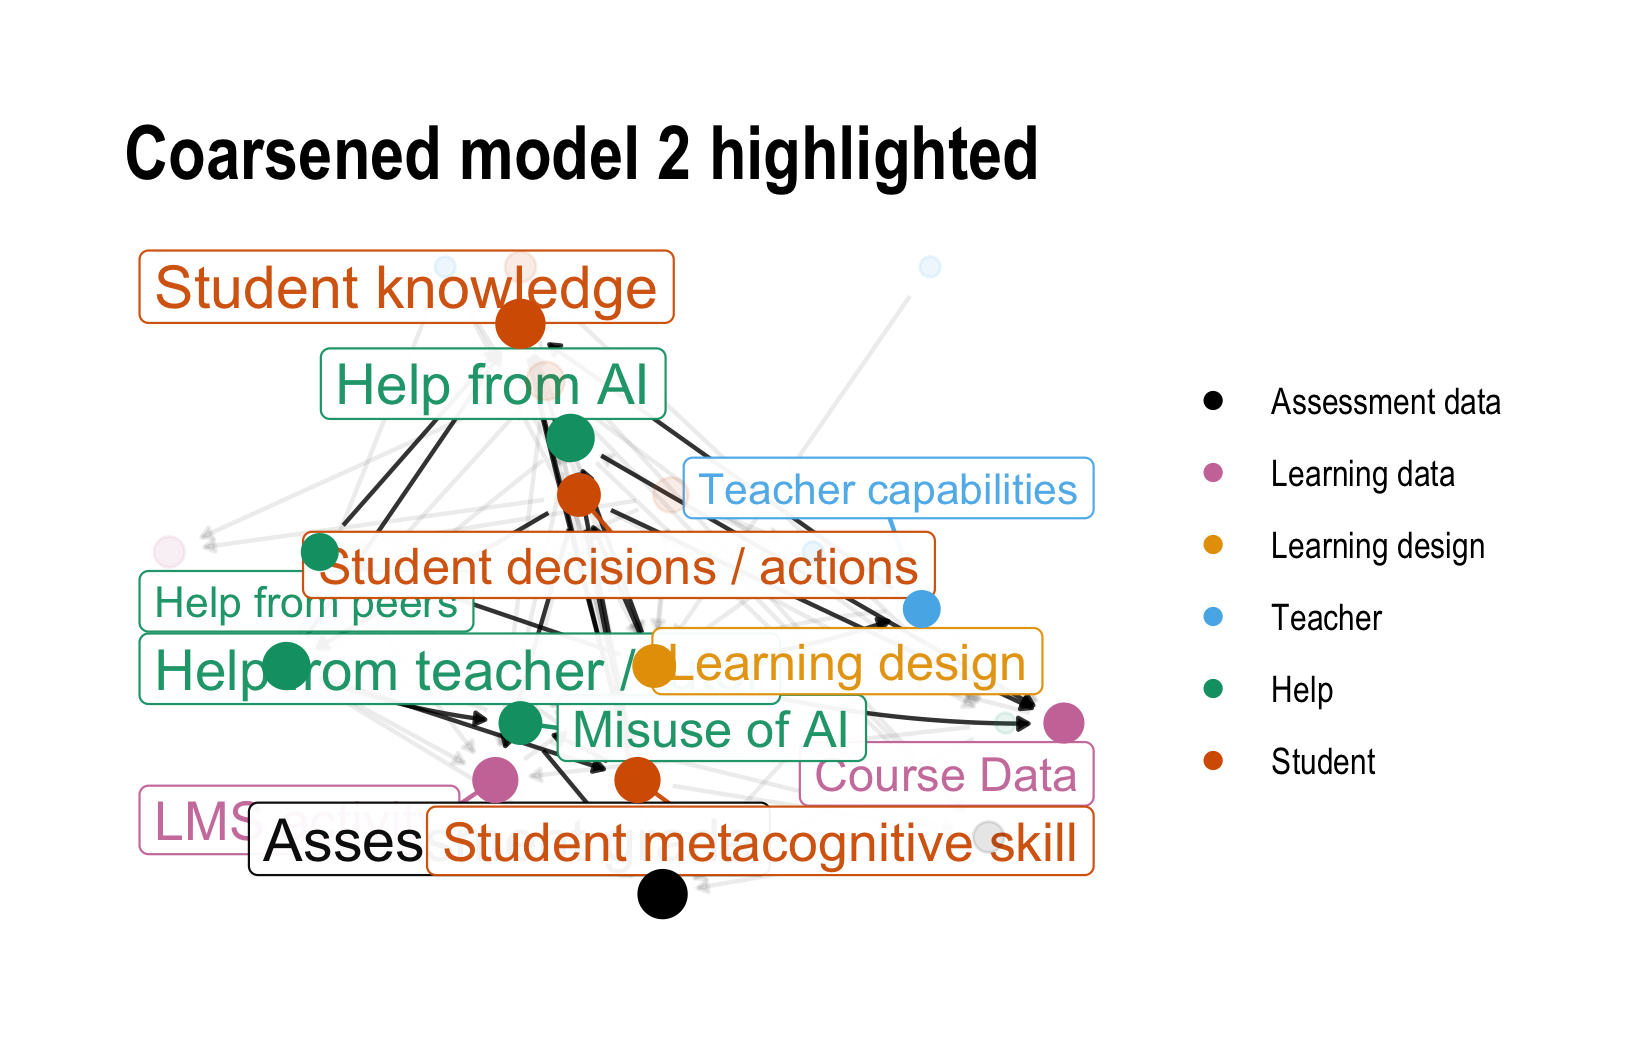
\includegraphics[keepaspectratio]{elicited-DAG-analysis_files/figure-pdf/unnamed-chunk-33-2.png}}

\begin{Shaded}
\begin{Highlighting}[]
\FunctionTok{p\_coarse\_show\_and\_save}\NormalTok{(}\DecValTok{3}\NormalTok{)}
\end{Highlighting}
\end{Shaded}

\pandocbounded{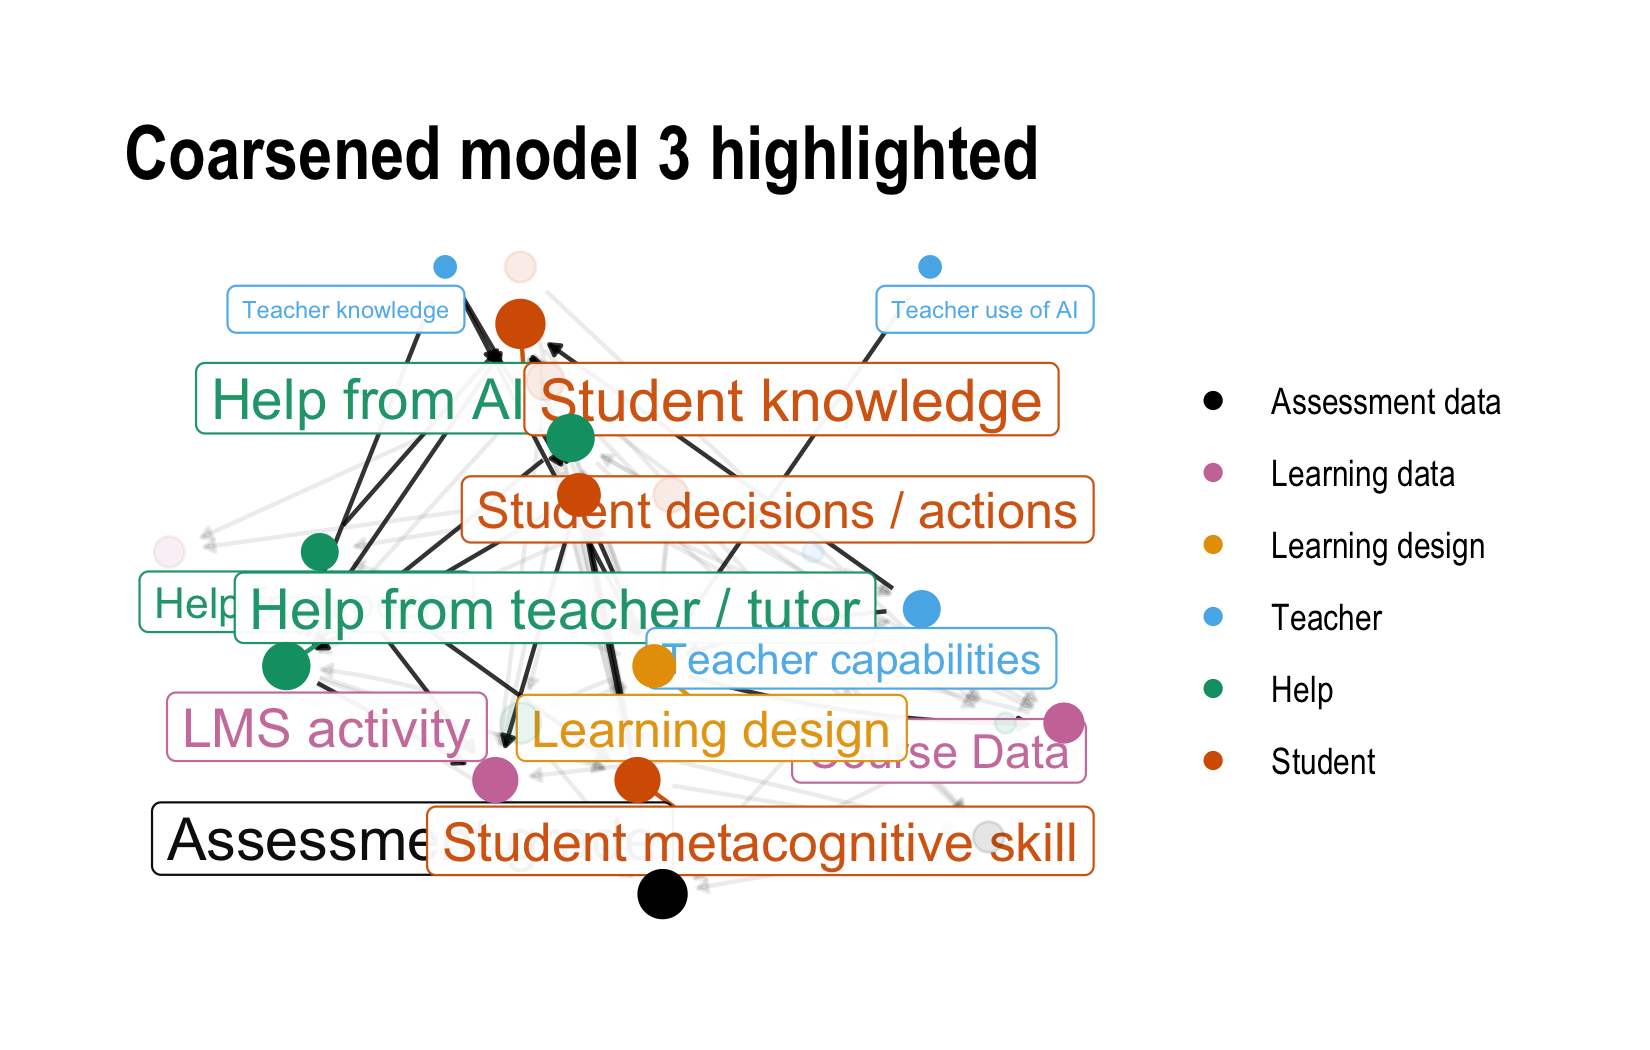
\includegraphics[keepaspectratio]{elicited-DAG-analysis_files/figure-pdf/unnamed-chunk-33-3.png}}

\begin{Shaded}
\begin{Highlighting}[]
\FunctionTok{p\_coarse\_show\_and\_save}\NormalTok{(}\DecValTok{4}\NormalTok{)}
\end{Highlighting}
\end{Shaded}

\pandocbounded{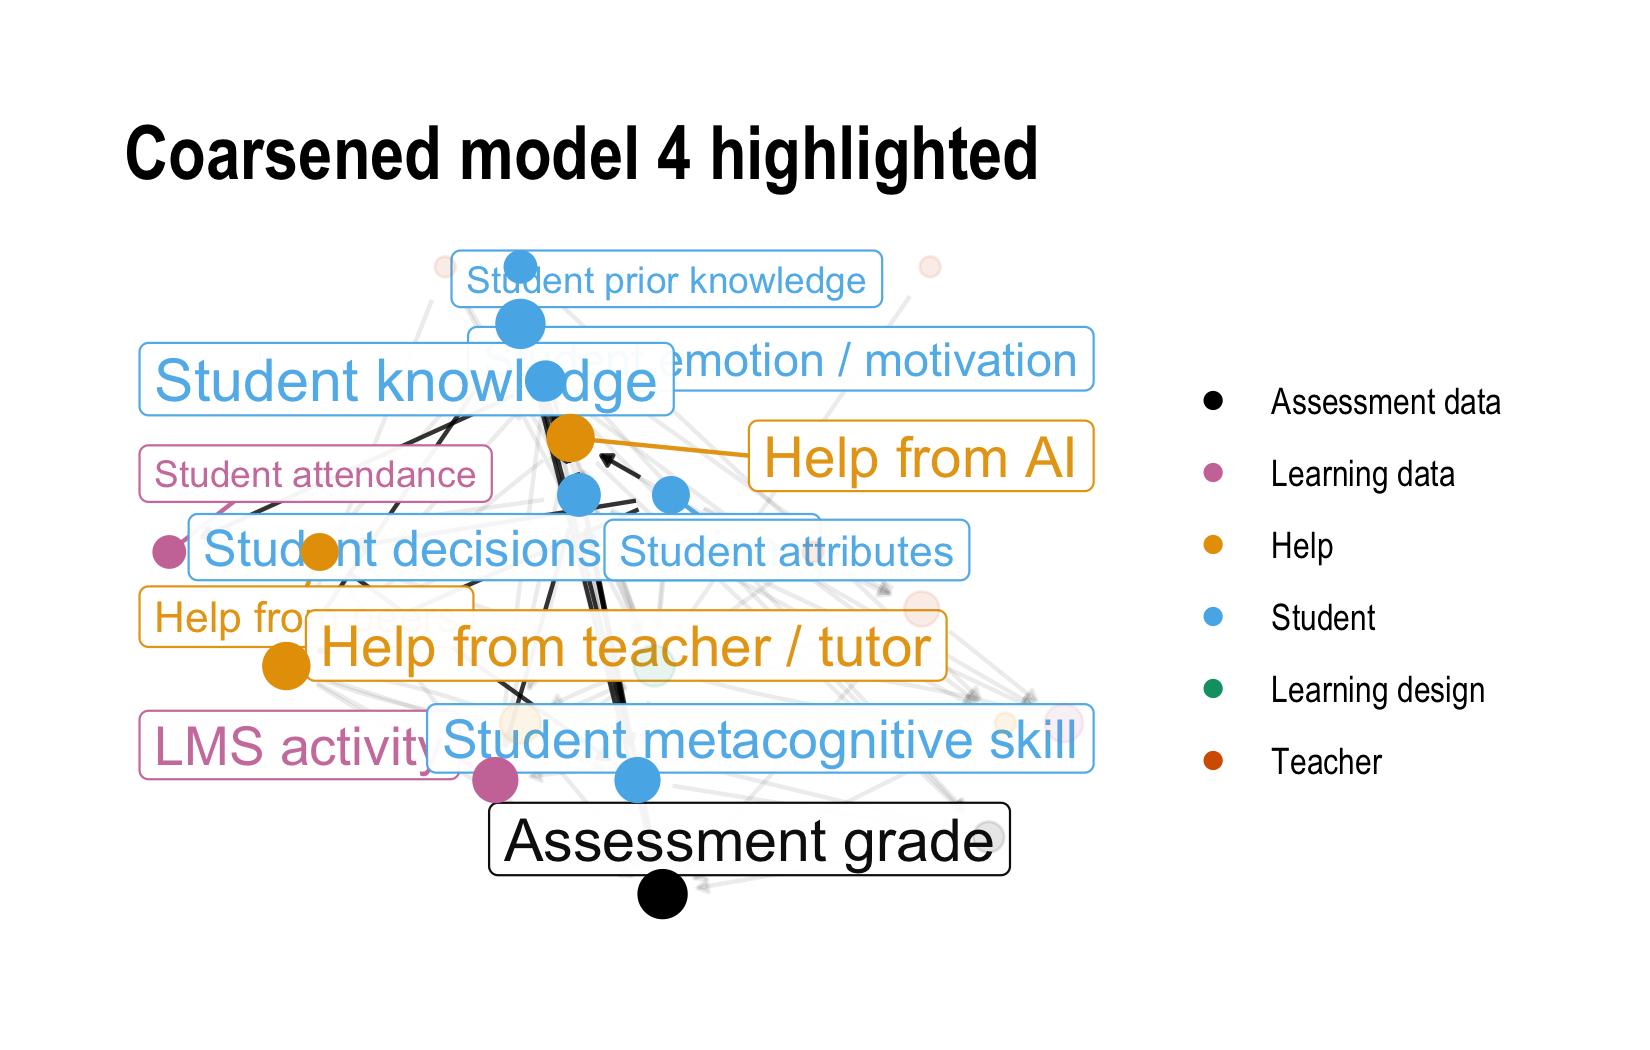
\includegraphics[keepaspectratio]{elicited-DAG-analysis_files/figure-pdf/unnamed-chunk-33-4.png}}

\begin{Shaded}
\begin{Highlighting}[]
\FunctionTok{p\_coarse\_show\_and\_save}\NormalTok{(}\DecValTok{5}\NormalTok{)}
\end{Highlighting}
\end{Shaded}

\pandocbounded{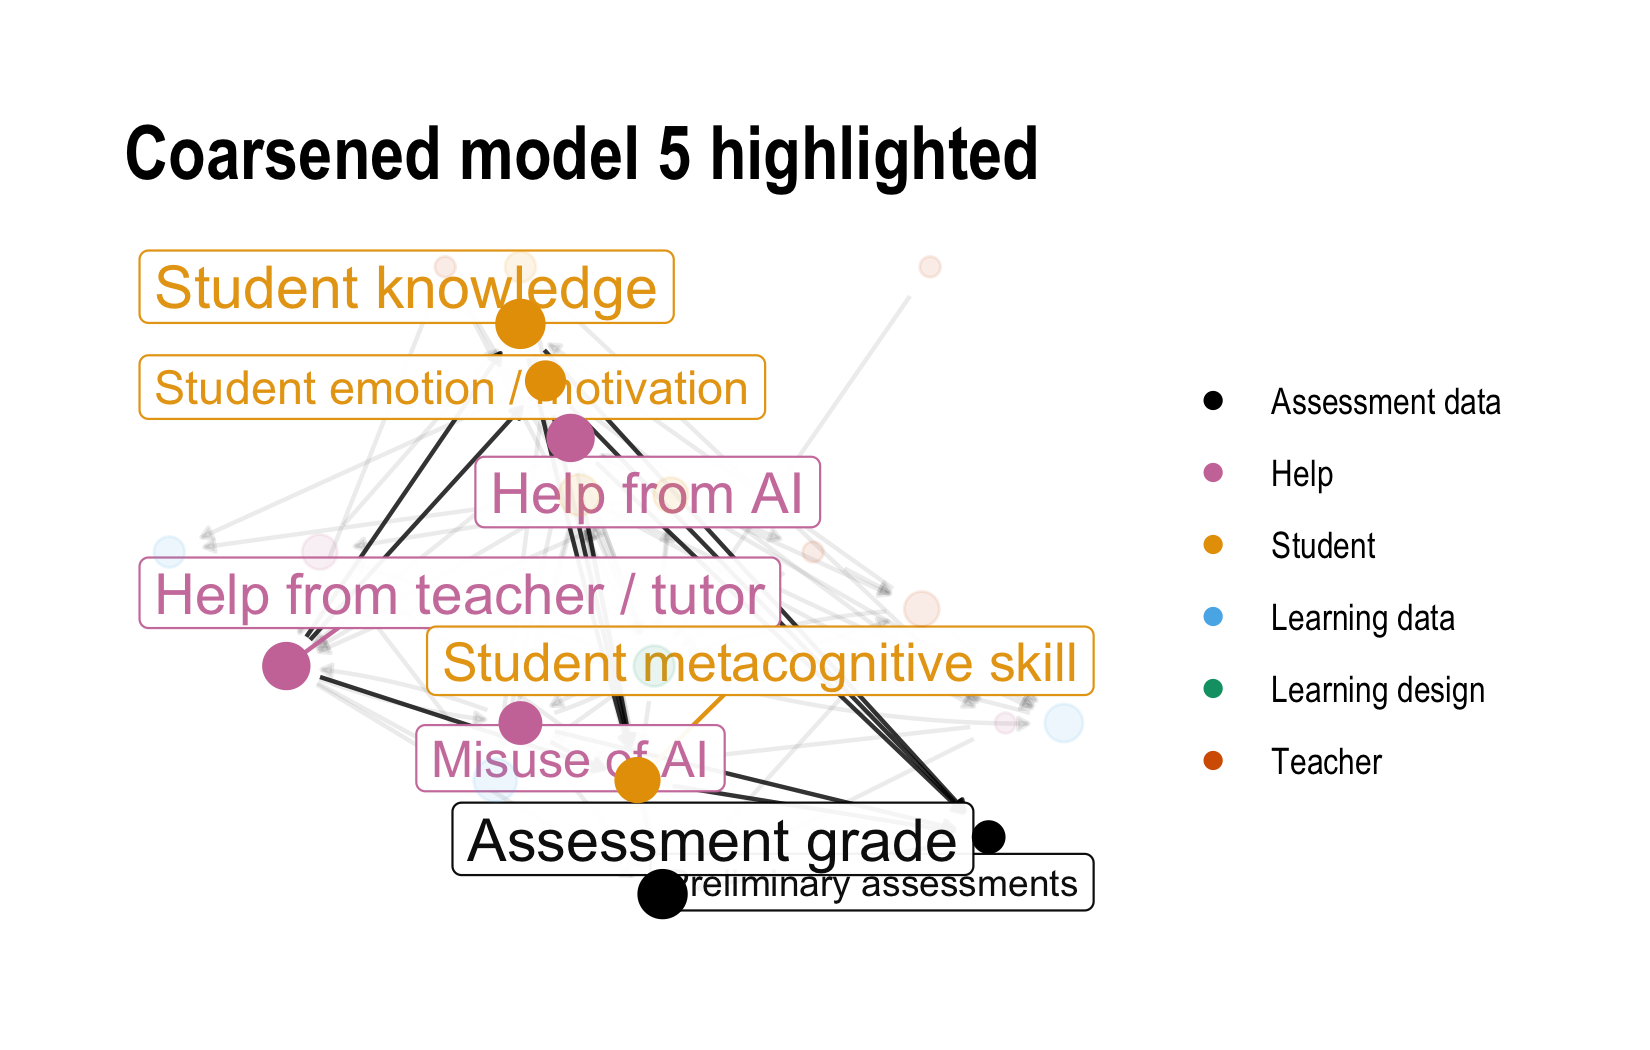
\includegraphics[keepaspectratio]{elicited-DAG-analysis_files/figure-pdf/unnamed-chunk-33-5.png}}

\begin{Shaded}
\begin{Highlighting}[]
\FunctionTok{p\_coarse\_show\_and\_save}\NormalTok{(}\DecValTok{6}\NormalTok{)}
\end{Highlighting}
\end{Shaded}

\pandocbounded{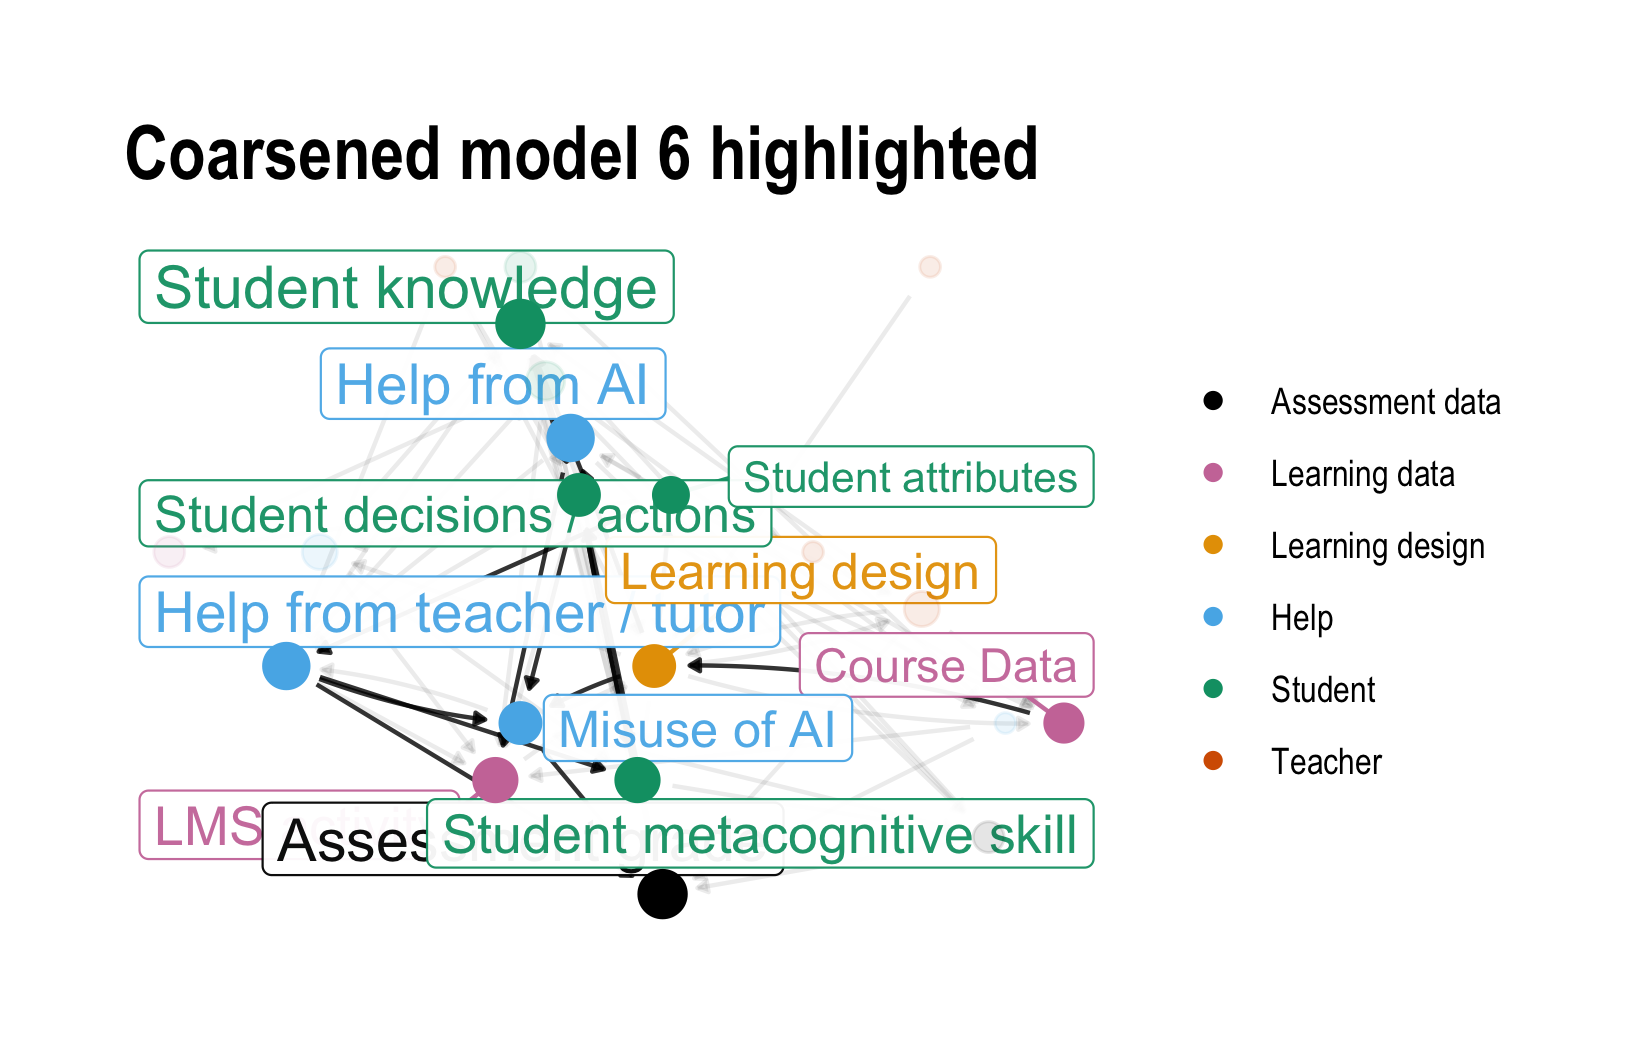
\includegraphics[keepaspectratio]{elicited-DAG-analysis_files/figure-pdf/unnamed-chunk-33-6.png}}

\begin{Shaded}
\begin{Highlighting}[]
\FunctionTok{p\_coarse\_show\_and\_save}\NormalTok{(}\DecValTok{7}\NormalTok{)}
\end{Highlighting}
\end{Shaded}

\pandocbounded{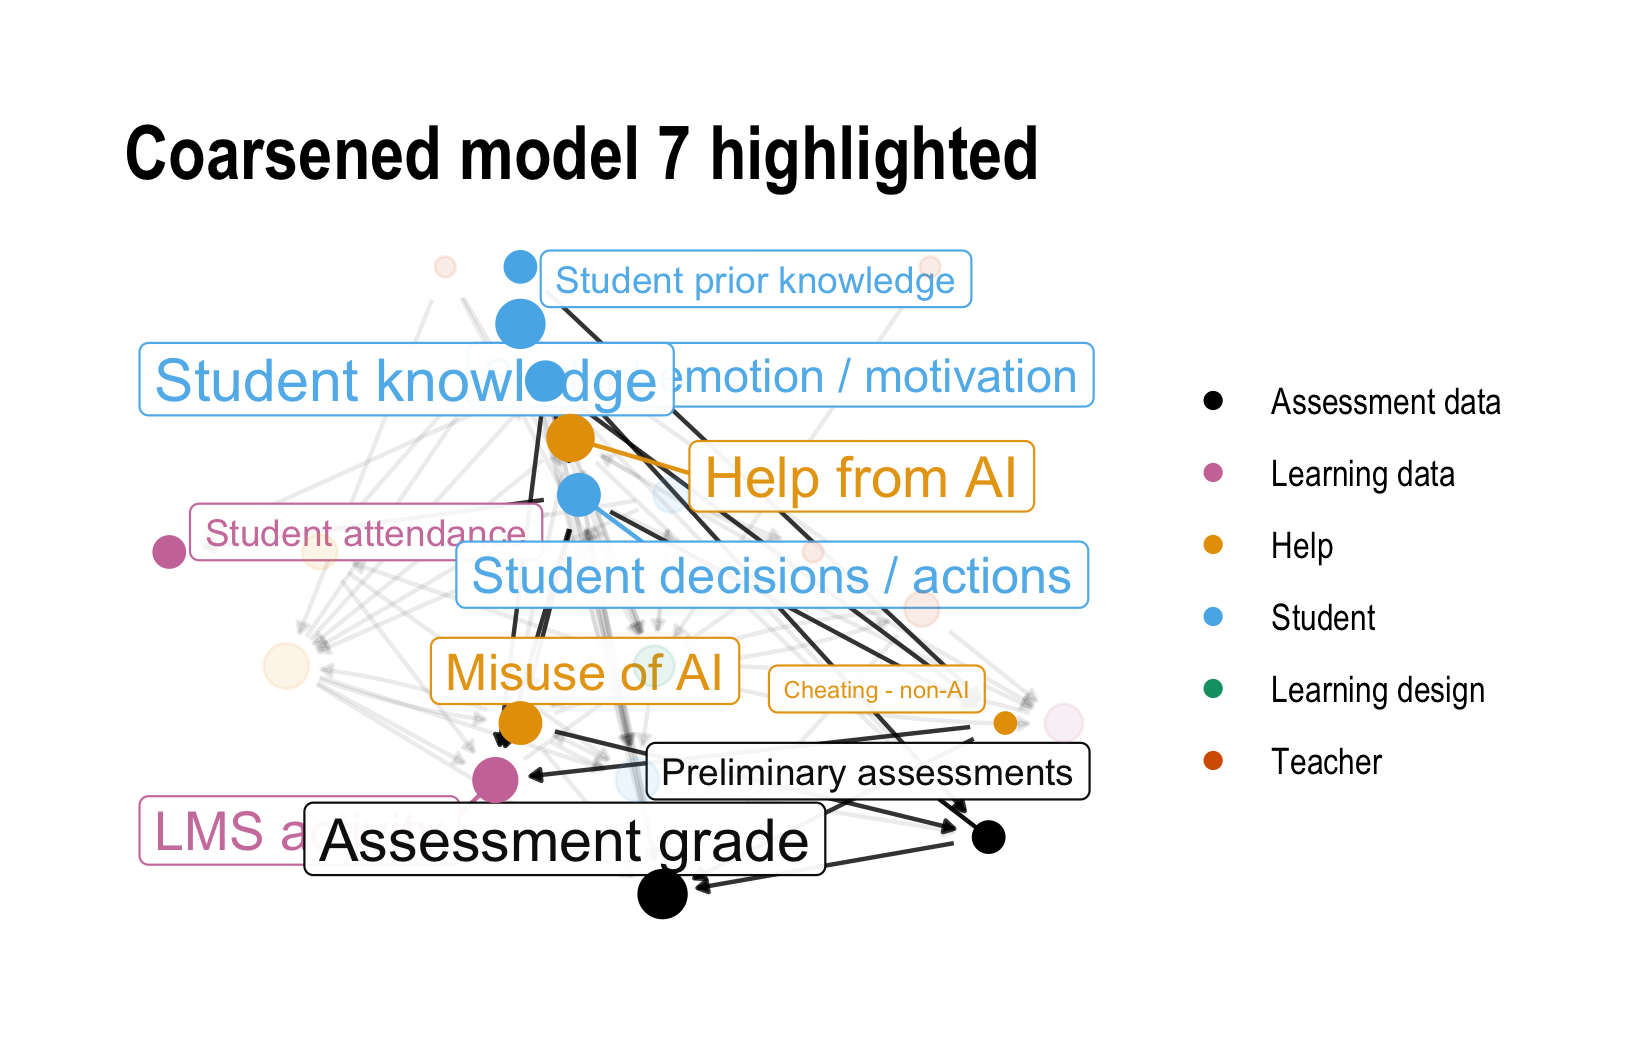
\includegraphics[keepaspectratio]{elicited-DAG-analysis_files/figure-pdf/unnamed-chunk-33-7.png}}

\begin{Shaded}
\begin{Highlighting}[]
\FunctionTok{p\_coarse\_show\_and\_save}\NormalTok{(}\DecValTok{8}\NormalTok{)}
\end{Highlighting}
\end{Shaded}

\pandocbounded{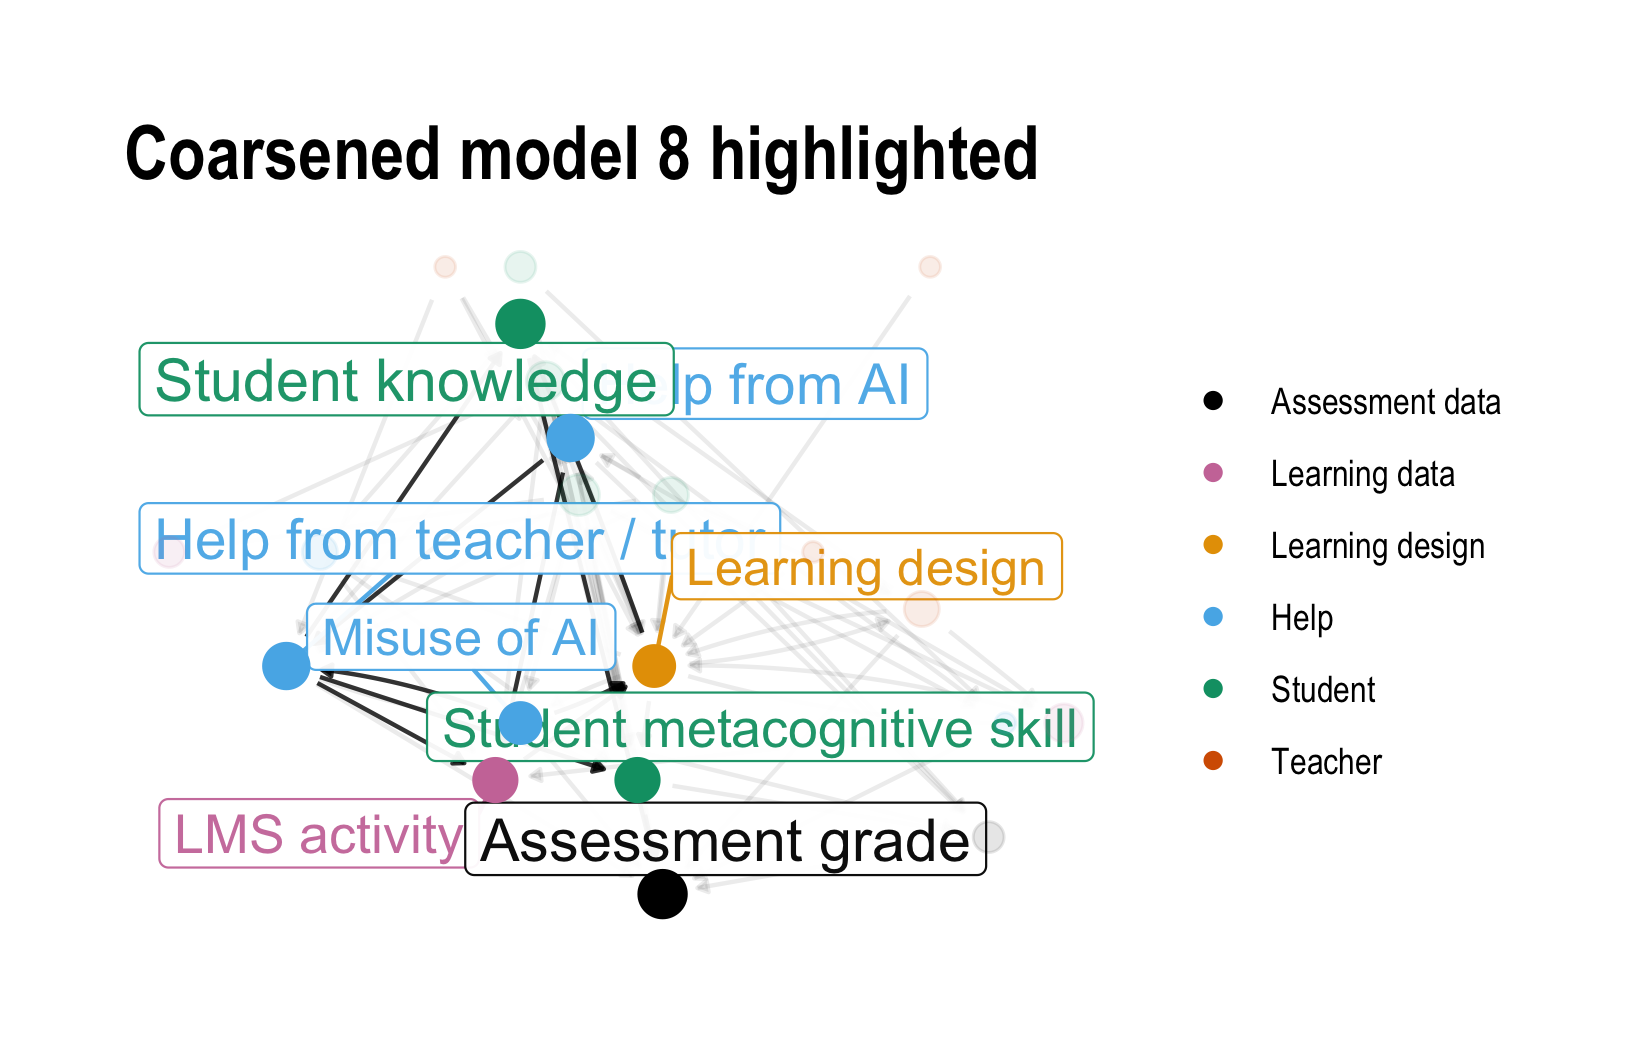
\includegraphics[keepaspectratio]{elicited-DAG-analysis_files/figure-pdf/unnamed-chunk-33-8.png}}

\subsubsection{Visualising coarsened
graphs}\label{visualising-coarsened-graphs}

\begin{Shaded}
\begin{Highlighting}[]
\NormalTok{merged\_coarse\_layout }\OtherTok{\textless{}{-}} 
\NormalTok{    merged\_all\_graph }\SpecialCharTok{|\textgreater{}} 
    \FunctionTok{g\_coarsen\_dag\_by\_ng}\NormalTok{() }\SpecialCharTok{|\textgreater{}} 
    \FunctionTok{create\_layout}\NormalTok{(}\AttributeTok{layout =} \StringTok{"sugiyama"}\NormalTok{) }\SpecialCharTok{|\textgreater{}} 
    \FunctionTok{mutate}\NormalTok{(}
        \AttributeTok{x =} \FunctionTok{case\_when}\NormalTok{(}
\NormalTok{            name }\SpecialCharTok{==} \StringTok{"CD.Att"} \SpecialCharTok{\textasciitilde{}} \FloatTok{18.5}\NormalTok{,}
\NormalTok{            name }\SpecialCharTok{==} \StringTok{"T.Aff.WrkLd"} \SpecialCharTok{\textasciitilde{}}\NormalTok{ x }\SpecialCharTok{{-}} \DecValTok{5}\NormalTok{,}
\NormalTok{            name }\SpecialCharTok{==} \StringTok{"H.AI.good"} \SpecialCharTok{\textasciitilde{}} \DecValTok{27}\NormalTok{,}
            \ConstantTok{TRUE} \SpecialCharTok{\textasciitilde{}}\NormalTok{ x),}
        \AttributeTok{y =} \FunctionTok{case\_when}\NormalTok{(}
\NormalTok{            name }\SpecialCharTok{==} \StringTok{"CD.Att"} \SpecialCharTok{\textasciitilde{}}\NormalTok{ y }\SpecialCharTok{+} \DecValTok{1}\NormalTok{,}
\NormalTok{            name }\SpecialCharTok{==} \StringTok{"Grade"} \SpecialCharTok{\textasciitilde{}}\NormalTok{ y }\SpecialCharTok{{-}} \FloatTok{2.5}\NormalTok{,}
\NormalTok{            name }\SpecialCharTok{==} \StringTok{"CD.Str"} \SpecialCharTok{\textasciitilde{}} \DecValTok{3}\NormalTok{,}
\NormalTok{            name }\SpecialCharTok{==} \StringTok{"S.EM"} \SpecialCharTok{\textasciitilde{}} \DecValTok{5}\NormalTok{,}
            \ConstantTok{TRUE} \SpecialCharTok{\textasciitilde{}}\NormalTok{ y)}
\NormalTok{           )}

\NormalTok{p\_temp }\OtherTok{\textless{}{-}}\NormalTok{ merged\_coarse\_layout }\SpecialCharTok{|\textgreater{}} 
     \FunctionTok{ggraph}\NormalTok{() }\SpecialCharTok{+}
        \FunctionTok{geom\_edge\_fan}\NormalTok{(}\FunctionTok{aes}\NormalTok{(}\AttributeTok{alpha =}\NormalTok{ edge\_w), }\AttributeTok{strength =} \FloatTok{0.2}\NormalTok{,}
            \AttributeTok{arrow =} \FunctionTok{arrow}\NormalTok{(}\AttributeTok{length =} \FunctionTok{unit}\NormalTok{(}\DecValTok{2}\NormalTok{, }\StringTok{\textquotesingle{}mm\textquotesingle{}}\NormalTok{)),}
            \AttributeTok{start\_cap =} \FunctionTok{circle}\NormalTok{(}\DecValTok{3}\NormalTok{, }\StringTok{\textquotesingle{}mm\textquotesingle{}}\NormalTok{),}
            \AttributeTok{end\_cap =} \FunctionTok{circle}\NormalTok{(}\DecValTok{3}\NormalTok{, }\StringTok{\textquotesingle{}mm\textquotesingle{}}\NormalTok{)) }\SpecialCharTok{+}
        \FunctionTok{geom\_node\_point}\NormalTok{(}\FunctionTok{aes}\NormalTok{(}\AttributeTok{colour =}\NormalTok{ node\_type, }\AttributeTok{size =}\NormalTok{ node\_w)) }\SpecialCharTok{+}
    \FunctionTok{scale\_color\_okabe\_ito}\NormalTok{(}\AttributeTok{order =} \FunctionTok{c}\NormalTok{(}\DecValTok{9}\NormalTok{, }\DecValTok{7}\NormalTok{,}\DecValTok{1}\NormalTok{, }\DecValTok{2}\NormalTok{,}\DecValTok{3}\NormalTok{, }\DecValTok{6}\NormalTok{, }\DecValTok{8}\NormalTok{,}\DecValTok{5}\NormalTok{, }\DecValTok{4}\NormalTok{)) }\SpecialCharTok{+}
        \CommentTok{\# scale\_color\_npg(drop = FALSE) +}
        \CommentTok{\# geom\_node\_text(aes(label = name, size = node\_w, alpha = node\_w), nudge\_y = {-}.5) +}
        \FunctionTok{theme\_graph}\NormalTok{() }\SpecialCharTok{+}
        \FunctionTok{scale\_edge\_alpha\_continuous}\NormalTok{(}\AttributeTok{range =} \FunctionTok{c}\NormalTok{(}\FloatTok{0.15}\NormalTok{,}\FloatTok{0.8}\NormalTok{)) }\SpecialCharTok{+}
        \FunctionTok{scale\_alpha\_continuous}\NormalTok{(}\AttributeTok{range =} \FunctionTok{c}\NormalTok{(}\FloatTok{0.2}\NormalTok{,}\FloatTok{0.6}\NormalTok{)) }\SpecialCharTok{+}
        \FunctionTok{theme}\NormalTok{(}\AttributeTok{legend.position =} \StringTok{"none"}\NormalTok{) }

\NormalTok{bc }\OtherTok{\textless{}{-}} \FunctionTok{ggplot\_build}\NormalTok{(p\_temp)}
\NormalTok{x\_limits\_course }\OtherTok{\textless{}{-}}\NormalTok{ bc}\SpecialCharTok{$}\NormalTok{layout}\SpecialCharTok{$}\NormalTok{panel\_params[[}\DecValTok{1}\NormalTok{]]}\SpecialCharTok{$}\NormalTok{x.range}
\NormalTok{y\_limits\_course }\OtherTok{\textless{}{-}}\NormalTok{ bc}\SpecialCharTok{$}\NormalTok{layout}\SpecialCharTok{$}\NormalTok{panel\_params[[}\DecValTok{1}\NormalTok{]]}\SpecialCharTok{$}\NormalTok{y.range}

\NormalTok{coarse\_plot\_from\_layout }\OtherTok{\textless{}{-}} \ControlFlowTok{function}\NormalTok{(lyt) \{}
\NormalTok{    lyt }\SpecialCharTok{|\textgreater{}} 
        \FunctionTok{ggraph}\NormalTok{() }\SpecialCharTok{+}
        \FunctionTok{geom\_edge\_fan}\NormalTok{(}\FunctionTok{aes}\NormalTok{(}\AttributeTok{alpha =}\NormalTok{ edge\_w), }\AttributeTok{strength =} \FloatTok{0.2}\NormalTok{,}
            \AttributeTok{arrow =} \FunctionTok{arrow}\NormalTok{(}\AttributeTok{length =} \FunctionTok{unit}\NormalTok{(}\DecValTok{2}\NormalTok{, }\StringTok{\textquotesingle{}mm\textquotesingle{}}\NormalTok{)),}
            \AttributeTok{start\_cap =} \FunctionTok{circle}\NormalTok{(}\DecValTok{3}\NormalTok{, }\StringTok{\textquotesingle{}mm\textquotesingle{}}\NormalTok{),}
            \AttributeTok{end\_cap =} \FunctionTok{circle}\NormalTok{(}\DecValTok{3}\NormalTok{, }\StringTok{\textquotesingle{}mm\textquotesingle{}}\NormalTok{)) }\SpecialCharTok{+}
        \FunctionTok{geom\_node\_point}\NormalTok{(}\FunctionTok{aes}\NormalTok{(}\AttributeTok{colour =}\NormalTok{ node\_type, }\AttributeTok{size =}\NormalTok{ node\_w)) }\SpecialCharTok{+}
        \FunctionTok{scale\_color\_okabe\_ito}\NormalTok{(}\AttributeTok{order =} \FunctionTok{c}\NormalTok{(}\DecValTok{9}\NormalTok{, }\DecValTok{7}\NormalTok{,}\DecValTok{1}\NormalTok{, }\DecValTok{2}\NormalTok{,}\DecValTok{3}\NormalTok{, }\DecValTok{6}\NormalTok{, }\DecValTok{8}\NormalTok{,}\DecValTok{5}\NormalTok{, }\DecValTok{4}\NormalTok{), }\AttributeTok{drop =} \ConstantTok{FALSE}\NormalTok{) }\SpecialCharTok{+}
        \CommentTok{\# ggsci::scale\_color\_npg(drop = FALSE) +}
        \CommentTok{\# geom\_node\_text(aes(label = name, size = node\_w, alpha = node\_w), nudge\_y = {-}.5) +}
        \FunctionTok{theme\_graph}\NormalTok{() }\SpecialCharTok{+}
        \FunctionTok{scale\_edge\_alpha\_continuous}\NormalTok{(}\AttributeTok{range =} \FunctionTok{c}\NormalTok{(}\FloatTok{0.15}\NormalTok{,}\FloatTok{0.8}\NormalTok{)) }\SpecialCharTok{+}
        \FunctionTok{scale\_alpha\_continuous}\NormalTok{(}\AttributeTok{range =} \FunctionTok{c}\NormalTok{(}\FloatTok{0.2}\NormalTok{,}\FloatTok{0.6}\NormalTok{)) }\SpecialCharTok{+}
        \FunctionTok{theme}\NormalTok{(}\AttributeTok{legend.position =} \StringTok{"none"}\NormalTok{) }\SpecialCharTok{+}
        \FunctionTok{xlim}\NormalTok{(x\_limits\_course) }\SpecialCharTok{+}
        \FunctionTok{ylim}\NormalTok{(y\_limits\_course)}
\NormalTok{\}}

\NormalTok{g\_plot\_coarse }\OtherTok{\textless{}{-}} \ControlFlowTok{function}\NormalTok{(g, }\AttributeTok{lyt =}\NormalTok{ merged\_coarse\_layout) \{}
    \FunctionTok{create\_layout}\NormalTok{(g, }\AttributeTok{layout =} \StringTok{"sugiyama"}\NormalTok{) }\SpecialCharTok{|\textgreater{}} 
        \FunctionTok{left\_join}\NormalTok{(lyt }\SpecialCharTok{|\textgreater{}} \FunctionTok{select}\NormalTok{(x,y,name, node\_type,node\_w), }\AttributeTok{by =} \StringTok{"name"}\NormalTok{,}
                  \AttributeTok{suffix =} \FunctionTok{c}\NormalTok{(}\StringTok{".default"}\NormalTok{, }\StringTok{""}\NormalTok{)) }\SpecialCharTok{|\textgreater{}} 
    \FunctionTok{coarse\_plot\_from\_layout}\NormalTok{()    }
\NormalTok{\}}

\NormalTok{pCoarseMerged }\OtherTok{\textless{}{-}}\NormalTok{ merged\_coarse\_layout }\SpecialCharTok{|\textgreater{}} 
    \FunctionTok{coarse\_plot\_from\_layout}\NormalTok{()}
\CommentTok{\# ggsave("dag\_merged\_course.svg", pCoarseMerged, , width = 6, height = 6)}
\end{Highlighting}
\end{Shaded}

Note the appearance of feedback loops - these are between S.Cp and S.Kn,
but also S.Cp and H.AI.evil. These metacognitive skills are clearly seen
as important feedback processes in this system.

\begin{Shaded}
\begin{Highlighting}[]
\NormalTok{pCoarseMerged }\SpecialCharTok{+} \FunctionTok{geom\_node\_text}\NormalTok{(}\FunctionTok{aes}\NormalTok{(}\AttributeTok{label =}\NormalTok{ name, }\AttributeTok{size =}\NormalTok{ node\_w, }\AttributeTok{alpha =}\NormalTok{ node\_w), }\AttributeTok{nudge\_x =} \DecValTok{1}\NormalTok{)}
\end{Highlighting}
\end{Shaded}

\begin{verbatim}
Warning: Removed 1 row containing missing values or values outside the scale range
(`geom_point()`).
\end{verbatim}

\pandocbounded{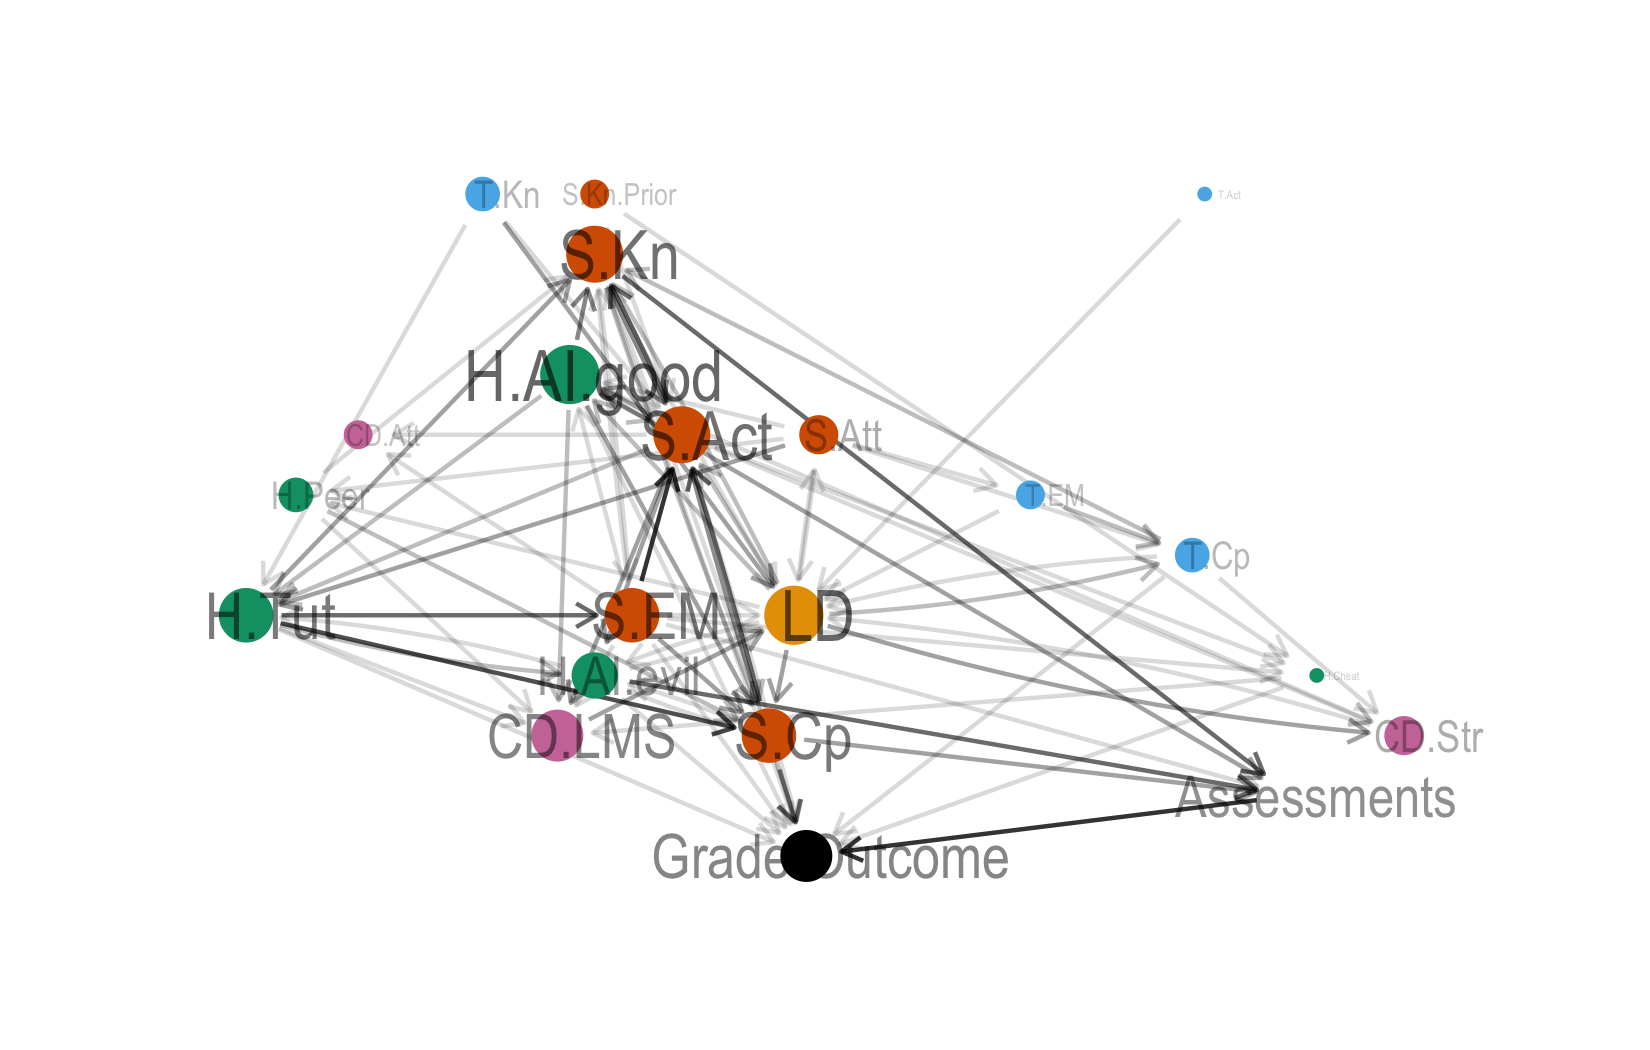
\includegraphics[keepaspectratio]{elicited-DAG-analysis_files/figure-pdf/unnamed-chunk-34-1.png}}

\begin{Shaded}
\begin{Highlighting}[]
\NormalTok{p1course }\OtherTok{\textless{}{-}} \FunctionTok{g\_coarsen\_dag\_by\_ng}\NormalTok{(tdag\_s1) }\SpecialCharTok{|\textgreater{}} \FunctionTok{g\_plot\_coarse}\NormalTok{()}
\NormalTok{p2course }\OtherTok{\textless{}{-}} \FunctionTok{g\_coarsen\_dag\_by\_ng}\NormalTok{(tdag\_s2) }\SpecialCharTok{|\textgreater{}} \FunctionTok{g\_plot\_coarse}\NormalTok{()}
\NormalTok{p3course }\OtherTok{\textless{}{-}} \FunctionTok{g\_coarsen\_dag\_by\_ng}\NormalTok{(tdag\_s3) }\SpecialCharTok{|\textgreater{}} \FunctionTok{g\_plot\_coarse}\NormalTok{()}
\NormalTok{p4course }\OtherTok{\textless{}{-}} \FunctionTok{g\_coarsen\_dag\_by\_ng}\NormalTok{(tdag\_s4) }\SpecialCharTok{|\textgreater{}} \FunctionTok{g\_plot\_coarse}\NormalTok{()}
\NormalTok{p5course }\OtherTok{\textless{}{-}} \FunctionTok{g\_coarsen\_dag\_by\_ng}\NormalTok{(tdag\_s5) }\SpecialCharTok{|\textgreater{}} \FunctionTok{g\_plot\_coarse}\NormalTok{()}
\NormalTok{p6course }\OtherTok{\textless{}{-}} \FunctionTok{g\_coarsen\_dag\_by\_ng}\NormalTok{(tdag\_s6) }\SpecialCharTok{|\textgreater{}} \FunctionTok{g\_plot\_coarse}\NormalTok{()}
\NormalTok{p7course }\OtherTok{\textless{}{-}} \FunctionTok{g\_coarsen\_dag\_by\_ng}\NormalTok{(tdag\_s7) }\SpecialCharTok{|\textgreater{}} \FunctionTok{g\_plot\_coarse}\NormalTok{()}
\NormalTok{p8course }\OtherTok{\textless{}{-}} \FunctionTok{g\_coarsen\_dag\_by\_ng}\NormalTok{(tdag\_s8) }\SpecialCharTok{|\textgreater{}} \FunctionTok{g\_plot\_coarse}\NormalTok{()}

\NormalTok{pAllcourse }\OtherTok{\textless{}{-}}\NormalTok{ (p1course }\SpecialCharTok{|}\NormalTok{ p2course }\SpecialCharTok{|}\NormalTok{ p3course }\SpecialCharTok{|}\NormalTok{ p4course) }\SpecialCharTok{/}\NormalTok{ (p5course }\SpecialCharTok{|}\NormalTok{ p6course }\SpecialCharTok{|}\NormalTok{ p7course }\SpecialCharTok{|}\NormalTok{ p8course)}
\CommentTok{\# ggsave("dags\_all\_course.svg", pAllcourse, width = 18, height = 9)}

\NormalTok{pAllcourse}
\end{Highlighting}
\end{Shaded}

\begin{verbatim}
Warning: Removed 1 row containing missing values or values outside the scale range
(`geom_point()`).
Removed 1 row containing missing values or values outside the scale range
(`geom_point()`).
\end{verbatim}

\pandocbounded{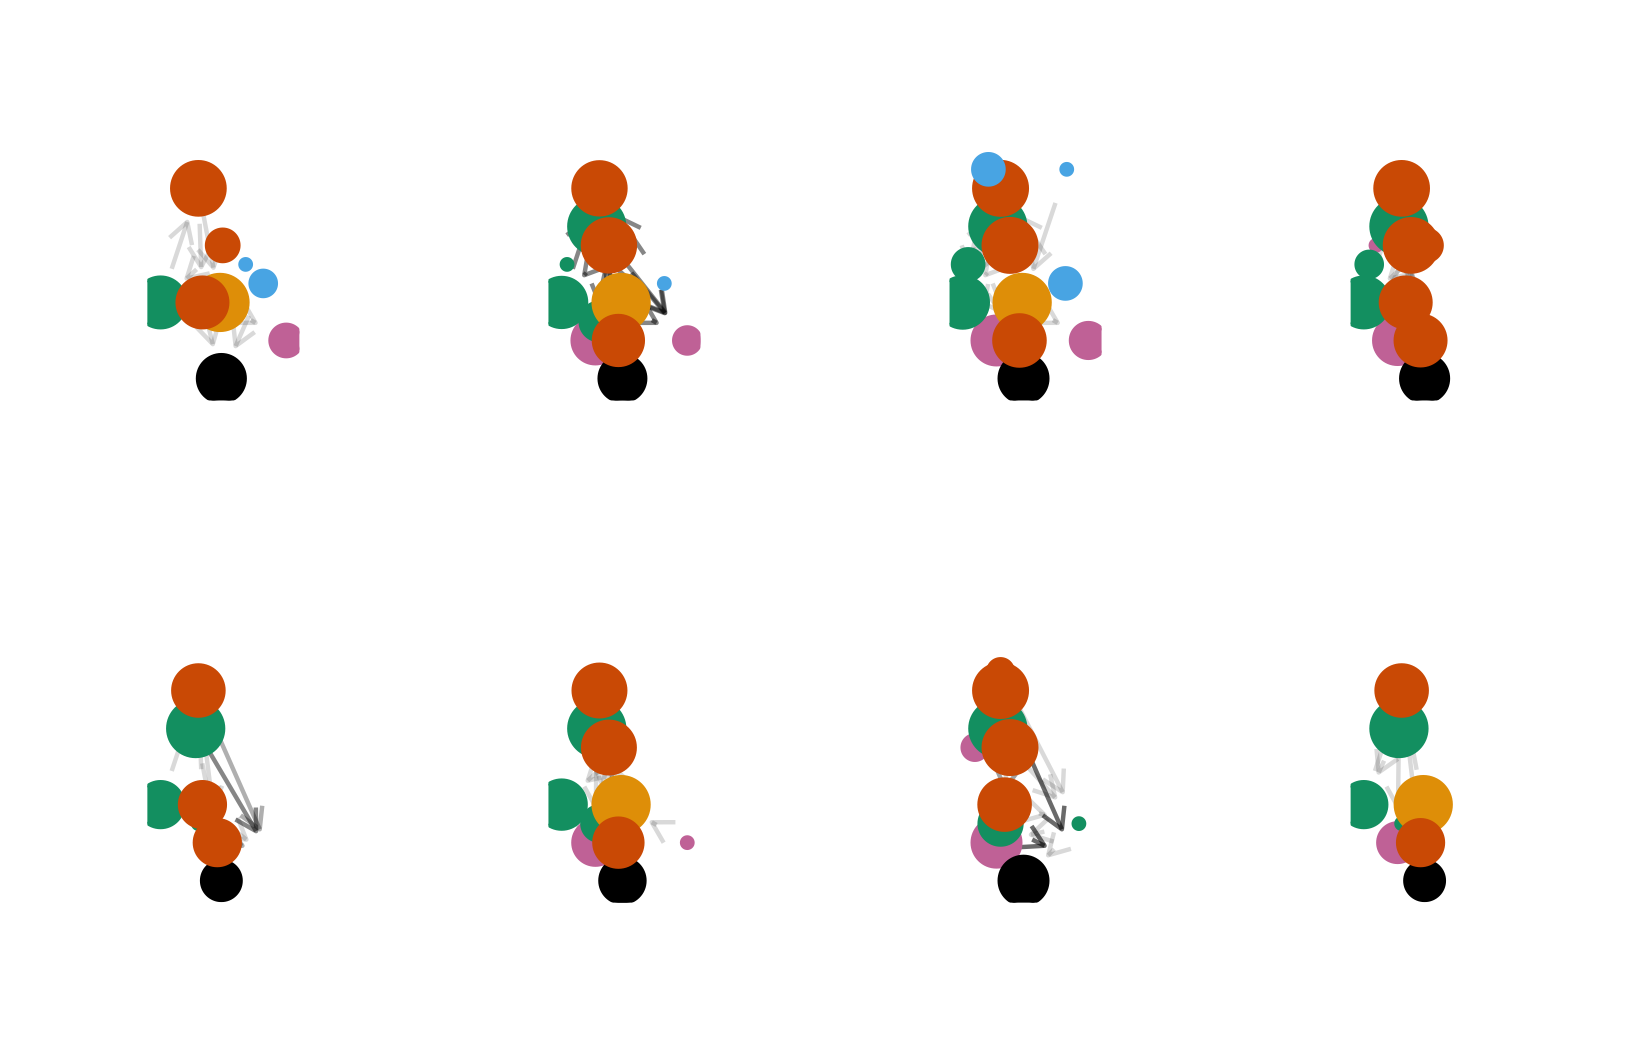
\includegraphics[keepaspectratio]{elicited-DAG-analysis_files/figure-pdf/unnamed-chunk-35-1.png}}

\begin{Shaded}
\begin{Highlighting}[]
\CommentTok{\# all node group edges}
\NormalTok{all\_edges }\SpecialCharTok{|\textgreater{}} 
    \FunctionTok{mutate}\NormalTok{(}
        \AttributeTok{from\_g =} \FunctionTok{code\_node\_group}\NormalTok{(from), }
        \AttributeTok{to\_g =} \FunctionTok{code\_node\_group}\NormalTok{(to)) }\SpecialCharTok{|\textgreater{}} 
    \FunctionTok{filter}\NormalTok{(to\_g }\SpecialCharTok{==} \StringTok{"LD"}\NormalTok{) }\SpecialCharTok{|\textgreater{}} 
    \FunctionTok{filter}\NormalTok{(from\_g }\SpecialCharTok{==} \StringTok{"CD.LMS"}\NormalTok{)}
\end{Highlighting}
\end{Shaded}

\begin{verbatim}
# A tibble: 3 x 5
  Model from   to            from_g to_g 
  <chr> <chr>  <chr>         <chr>  <chr>
1 s8    CD.LMS LD.Task.Code  CD.LMS LD   
2 s8    CD.LMS LD.Task.Prac  CD.LMS LD   
3 s8    CD.LMS LD.Task.Write CD.LMS LD   
\end{verbatim}

\paragraph{Figure: Consensus DAG}\label{figure-consensus-dag}

Most common node group patterns - nodes in at least half the models,
then looking at the resulting graph of node-groups.

\begin{Shaded}
\begin{Highlighting}[]
\NormalTok{node\_list\_majority\_of\_models }\OtherTok{\textless{}{-}} 
\NormalTok{    all\_nodes }\SpecialCharTok{|\textgreater{}} 
    \FunctionTok{count}\NormalTok{(name) }\SpecialCharTok{|\textgreater{}} 
    \FunctionTok{filter}\NormalTok{(n }\SpecialCharTok{\textgreater{}=} \DecValTok{4}\NormalTok{) }\SpecialCharTok{|\textgreater{}} 
    \FunctionTok{pull}\NormalTok{(name)}

\NormalTok{coarse\_filtered\_graph\_temp }\OtherTok{\textless{}{-}} 
\NormalTok{    merged\_all\_graph }\SpecialCharTok{|\textgreater{}} 
    \FunctionTok{activate}\NormalTok{(}\StringTok{"nodes"}\NormalTok{) }\SpecialCharTok{|\textgreater{}} 
    \FunctionTok{filter}\NormalTok{(name }\SpecialCharTok{\%in\%}\NormalTok{ node\_list\_majority\_of\_models)}

\NormalTok{coarse\_filtered\_graph }\OtherTok{\textless{}{-}} \FunctionTok{tbl\_graph}\NormalTok{(}
    \AttributeTok{nodes =}\NormalTok{ coarse\_filtered\_graph\_temp }\SpecialCharTok{\%N\textgreater{}\%}
        \FunctionTok{as\_tibble}\NormalTok{() }\SpecialCharTok{|\textgreater{}} 
        \FunctionTok{mutate}\NormalTok{(}\AttributeTok{name =} \FunctionTok{code\_node\_group}\NormalTok{(name),}
               \AttributeTok{node\_type =} \FunctionTok{code\_node\_type}\NormalTok{(name)) ,}
    \AttributeTok{edges =}\NormalTok{ coarse\_filtered\_graph\_temp }\SpecialCharTok{\%E\textgreater{}\%}
        \FunctionTok{as\_tibble}\NormalTok{() }\SpecialCharTok{\%\textgreater{}\%}
        \FunctionTok{mutate}\NormalTok{(}
            \AttributeTok{from =}\NormalTok{ coarse\_filtered\_graph\_temp }\SpecialCharTok{\%N\textgreater{}\%} \FunctionTok{pull}\NormalTok{(name) }\SpecialCharTok{\%\textgreater{}\%}\NormalTok{ .[from],}
            \AttributeTok{to   =}\NormalTok{ coarse\_filtered\_graph\_temp }\SpecialCharTok{\%N\textgreater{}\%} \FunctionTok{pull}\NormalTok{(name) }\SpecialCharTok{\%\textgreater{}\%}\NormalTok{ .[to]}
\NormalTok{        ) }\SpecialCharTok{\%\textgreater{}\%}
        \FunctionTok{select}\NormalTok{(from, to, edge\_w) }\SpecialCharTok{|\textgreater{}} 
        \FunctionTok{mutate}\NormalTok{(}\FunctionTok{across}\NormalTok{(from}\SpecialCharTok{:}\NormalTok{to, code\_node\_group))) }\SpecialCharTok{|\textgreater{}} 
    \FunctionTok{activate}\NormalTok{(edges) }\SpecialCharTok{|\textgreater{}} 
    \FunctionTok{mutate}\NormalTok{(}
        \AttributeTok{switched =} \FunctionTok{map\_lgl}\NormalTok{(}\FunctionTok{row\_number}\NormalTok{(), }\ControlFlowTok{function}\NormalTok{(i) \{}
\NormalTok{            from\_i }\OtherTok{\textless{}{-}} \FunctionTok{.E}\NormalTok{()}\SpecialCharTok{$}\NormalTok{from[i]}
\NormalTok{            to\_i   }\OtherTok{\textless{}{-}} \FunctionTok{.E}\NormalTok{()}\SpecialCharTok{$}\NormalTok{to[i]}
            \FunctionTok{any}\NormalTok{(from }\SpecialCharTok{==}\NormalTok{ to\_i }\SpecialCharTok{\&}\NormalTok{ to }\SpecialCharTok{==}\NormalTok{ from\_i)}
\NormalTok{        \})}
\NormalTok{    ) }
\end{Highlighting}
\end{Shaded}

\begin{Shaded}
\begin{Highlighting}[]
\CommentTok{\# Old {-} not used}
\NormalTok{lyt\_top\_node\_groups }\OtherTok{\textless{}{-}} \FunctionTok{create\_layout}\NormalTok{(coarse\_filtered\_graph, }\AttributeTok{layout =} \StringTok{"sugiyama"}\NormalTok{) }\SpecialCharTok{|\textgreater{}} 
    \FunctionTok{mutate}\NormalTok{(}
        \AttributeTok{x =} \FunctionTok{case\_when}\NormalTok{(}
\NormalTok{            nice\_name }\SpecialCharTok{==} \StringTok{"Student subject knowledge"} \SpecialCharTok{\textasciitilde{}} \FloatTok{0.5}\NormalTok{,}
\NormalTok{            nice\_name }\SpecialCharTok{==} \StringTok{"Assessment grade"} \SpecialCharTok{\textasciitilde{}} \FloatTok{0.5}\NormalTok{,}
\NormalTok{            nice\_name }\SpecialCharTok{==} \StringTok{"Help from teacher / tutor"} \SpecialCharTok{\textasciitilde{}} \DecValTok{1}\NormalTok{,}
\NormalTok{            nice\_name }\SpecialCharTok{==} \StringTok{"Task design"} \SpecialCharTok{\textasciitilde{}} \FloatTok{0.5}\NormalTok{,}
            \ConstantTok{TRUE} \SpecialCharTok{\textasciitilde{}}\NormalTok{ x}
\NormalTok{        ),}
        \AttributeTok{y =} \FunctionTok{case\_when}\NormalTok{(}
\NormalTok{            nice\_name }\SpecialCharTok{==} \StringTok{"Student subject knowledge"} \SpecialCharTok{\textasciitilde{}} \FloatTok{2.5}\NormalTok{,}
            \CommentTok{\# nice\_name == "Assessment grade" \textasciitilde{} 0.5,}
\NormalTok{            nice\_name }\SpecialCharTok{==} \StringTok{"LMS activity"} \SpecialCharTok{\textasciitilde{}} \DecValTok{1}\NormalTok{,}
\NormalTok{            nice\_name }\SpecialCharTok{==} \StringTok{"Task design"} \SpecialCharTok{\textasciitilde{}} \DecValTok{4}\NormalTok{,}
            \ConstantTok{TRUE} \SpecialCharTok{\textasciitilde{}}\NormalTok{ y}
\NormalTok{        )}
\NormalTok{    )}

\NormalTok{p\_top\_node\_groups }\OtherTok{\textless{}{-}} \FunctionTok{ggraph}\NormalTok{(lyt\_top\_node\_groups) }\SpecialCharTok{+}
    \FunctionTok{geom\_edge\_fan}\NormalTok{(}\FunctionTok{aes}\NormalTok{(}\AttributeTok{edge\_linetype =} \FunctionTok{factor}\NormalTok{(switched), }\AttributeTok{alpha =}\NormalTok{ edge\_w, ), }\CommentTok{\# alpha = edge\_w, }
                  \AttributeTok{strength =} \FloatTok{0.8}\NormalTok{,}
                  \AttributeTok{arrow =} \FunctionTok{arrow}\NormalTok{(}\AttributeTok{length =} \FunctionTok{unit}\NormalTok{(}\DecValTok{2}\NormalTok{, }\StringTok{\textquotesingle{}mm\textquotesingle{}}\NormalTok{), }\AttributeTok{type =} \StringTok{"closed"}\NormalTok{),}
                  \AttributeTok{start\_cap =} \FunctionTok{circle}\NormalTok{(}\DecValTok{3}\NormalTok{, }\StringTok{\textquotesingle{}mm\textquotesingle{}}\NormalTok{),}
                  \AttributeTok{end\_cap =} \FunctionTok{circle}\NormalTok{(}\DecValTok{3}\NormalTok{, }\StringTok{\textquotesingle{}mm\textquotesingle{}}\NormalTok{)) }\SpecialCharTok{+}
    \FunctionTok{geom\_node\_point}\NormalTok{(}\FunctionTok{aes}\NormalTok{(}\AttributeTok{colour =}\NormalTok{ node\_type, }\AttributeTok{size =}\NormalTok{ node\_w)) }\SpecialCharTok{+}
\NormalTok{        ggsci}\SpecialCharTok{::}\FunctionTok{scale\_color\_npg}\NormalTok{(}\AttributeTok{drop =} \ConstantTok{FALSE}\NormalTok{) }\SpecialCharTok{+}
        \CommentTok{\# geom\_node\_text(aes(label = name, size = node\_w, alpha = node\_w), nudge\_y = {-}.5) +}
        \FunctionTok{theme\_graph}\NormalTok{() }\SpecialCharTok{+}
        \FunctionTok{scale\_edge\_alpha\_continuous}\NormalTok{(}\AttributeTok{range =} \FunctionTok{c}\NormalTok{(}\FloatTok{0.15}\NormalTok{,}\FloatTok{0.8}\NormalTok{)) }\SpecialCharTok{+}
        \FunctionTok{scale\_alpha\_continuous}\NormalTok{(}\AttributeTok{range =} \FunctionTok{c}\NormalTok{(}\FloatTok{0.2}\NormalTok{,}\FloatTok{0.9}\NormalTok{)) }\SpecialCharTok{+}
        \FunctionTok{theme}\NormalTok{(}\AttributeTok{legend.position =} \StringTok{"none"}\NormalTok{) }\SpecialCharTok{+}
    \FunctionTok{geom\_node\_text}\NormalTok{(}\FunctionTok{aes}\NormalTok{(}\AttributeTok{label =}\NormalTok{ nice\_name, }\AttributeTok{colour =}\NormalTok{ node\_type), }
                   \AttributeTok{alpha =} \FloatTok{0.9}\NormalTok{, }\AttributeTok{nudge\_y =} \SpecialCharTok{{-}}\NormalTok{.}\DecValTok{3}\NormalTok{, }\AttributeTok{repel =}\NormalTok{ T)}

\CommentTok{\# p\_top\_node\_groups}
\CommentTok{\# ggsave("figures/FIG{-}{-}consensus{-}DAG.png", p\_top\_node\_groups, dpi = 600, height = 4, width = 6)}
\end{Highlighting}
\end{Shaded}

Weighting by num of models instead This one uses only nodes that are in
the majority of models, then coarsens the graph, then aggregates edges
based on the number of models that they appear in. The edges must also
appear in at least 2 models

\begin{Shaded}
\begin{Highlighting}[]
\NormalTok{node\_list\_majority\_of\_models }\OtherTok{\textless{}{-}} 
\NormalTok{    all\_nodes }\SpecialCharTok{|\textgreater{}} 
    \FunctionTok{count}\NormalTok{(name) }\SpecialCharTok{|\textgreater{}} 
    \FunctionTok{filter}\NormalTok{(n }\SpecialCharTok{\textgreater{}=} \DecValTok{4}\NormalTok{) }\SpecialCharTok{|\textgreater{}} 
    \FunctionTok{pull}\NormalTok{(name)}

\NormalTok{coarse\_filtered\_graph\_ng\_filled }\OtherTok{\textless{}{-}} 
    \FunctionTok{tbl\_graph}\NormalTok{( }\CommentTok{\# only nodes that are in most models (4 or more)}
        \AttributeTok{nodes =}\NormalTok{ all\_nodes }\SpecialCharTok{|\textgreater{}} 
            \FunctionTok{filter}\NormalTok{(name }\SpecialCharTok{\%in\%}\NormalTok{ node\_list\_majority\_of\_models) }\SpecialCharTok{|\textgreater{}} 
            \FunctionTok{mutate}\NormalTok{( }\CommentTok{\# but then coarsen into node groups}
                \AttributeTok{node\_group =} \FunctionTok{code\_node\_group}\NormalTok{(name),}
                   \AttributeTok{node\_type =} \FunctionTok{code\_node\_type}\NormalTok{(name)) }\SpecialCharTok{|\textgreater{}} 
            \FunctionTok{count}\NormalTok{(node\_group, node\_type) }\SpecialCharTok{|\textgreater{}} 
            \FunctionTok{rename}\NormalTok{(}\AttributeTok{node\_w =}\NormalTok{ n),}
        \AttributeTok{edges =}\NormalTok{     all\_edges }\SpecialCharTok{|\textgreater{}} \CommentTok{\# Only edges between node groups...}
            \FunctionTok{mutate}\NormalTok{(}\FunctionTok{across}\NormalTok{(from}\SpecialCharTok{:}\NormalTok{to, code\_node\_group)) }\SpecialCharTok{|\textgreater{}}
            \FunctionTok{distinct}\NormalTok{(Model, from, to) }\SpecialCharTok{|\textgreater{}} 
            \FunctionTok{count}\NormalTok{(from, to) }\SpecialCharTok{|\textgreater{}}
            \CommentTok{\# filter(n \textgreater{} 1) |\textgreater{} \# ...that occur in at least two models}
            \FunctionTok{filter}\NormalTok{(from }\SpecialCharTok{\%in\%} \FunctionTok{code\_node\_group}\NormalTok{(node\_list\_majority\_of\_models)) }\SpecialCharTok{|\textgreater{}}
            \FunctionTok{filter}\NormalTok{(to }\SpecialCharTok{\%in\%} \FunctionTok{code\_node\_group}\NormalTok{(node\_list\_majority\_of\_models)) }\SpecialCharTok{|\textgreater{}}
            \FunctionTok{rename}\NormalTok{(}\AttributeTok{edge\_w =}\NormalTok{ n)) }\SpecialCharTok{|\textgreater{}} 
    \FunctionTok{activate}\NormalTok{(}\StringTok{"edges"}\NormalTok{) }\SpecialCharTok{|\textgreater{}} 
    \FunctionTok{mutate}\NormalTok{(}
        \AttributeTok{switched =} \FunctionTok{map\_lgl}\NormalTok{(}\FunctionTok{row\_number}\NormalTok{(), }\ControlFlowTok{function}\NormalTok{(i) \{}
\NormalTok{            from\_i }\OtherTok{\textless{}{-}} \FunctionTok{.E}\NormalTok{()}\SpecialCharTok{$}\NormalTok{from[i]}
\NormalTok{            to\_i   }\OtherTok{\textless{}{-}} \FunctionTok{.E}\NormalTok{()}\SpecialCharTok{$}\NormalTok{to[i]}
            \FunctionTok{any}\NormalTok{(from }\SpecialCharTok{==}\NormalTok{ to\_i }\SpecialCharTok{\&}\NormalTok{ to }\SpecialCharTok{==}\NormalTok{ from\_i)}
\NormalTok{        \})}
\NormalTok{    ) }\SpecialCharTok{|\textgreater{}} 
    \FunctionTok{activate}\NormalTok{(}\StringTok{"nodes"}\NormalTok{) }\SpecialCharTok{|\textgreater{}} 
    \FunctionTok{inner\_join}\NormalTok{(node\_group\_nice\_name)}
\end{Highlighting}
\end{Shaded}

\begin{verbatim}
Joining with `by = join_by(node_group)`
\end{verbatim}

Filtered - edges must be in at least 2 models

\begin{Shaded}
\begin{Highlighting}[]
\NormalTok{lyt\_coarse\_filtered\_ng\_filtered }\OtherTok{\textless{}{-}} \FunctionTok{create\_layout}\NormalTok{(}
\NormalTok{    coarse\_filtered\_graph\_ng\_filled }\SpecialCharTok{|\textgreater{}} 
        \FunctionTok{activate}\NormalTok{(}\StringTok{"edges"}\NormalTok{) }\SpecialCharTok{|\textgreater{}} 
        \FunctionTok{filter}\NormalTok{(edge\_w }\SpecialCharTok{\textgreater{}} \DecValTok{1}\NormalTok{) }\SpecialCharTok{|\textgreater{}} 
        \FunctionTok{mutate}\NormalTok{(}
            \AttributeTok{switched =} \FunctionTok{map\_lgl}\NormalTok{(}\FunctionTok{row\_number}\NormalTok{(), }\ControlFlowTok{function}\NormalTok{(i) \{}
\NormalTok{                from\_i }\OtherTok{\textless{}{-}} \FunctionTok{.E}\NormalTok{()}\SpecialCharTok{$}\NormalTok{from[i]}
\NormalTok{                to\_i   }\OtherTok{\textless{}{-}} \FunctionTok{.E}\NormalTok{()}\SpecialCharTok{$}\NormalTok{to[i]}
                \FunctionTok{any}\NormalTok{(from }\SpecialCharTok{==}\NormalTok{ to\_i }\SpecialCharTok{\&}\NormalTok{ to }\SpecialCharTok{==}\NormalTok{ from\_i)}
\NormalTok{            \})}
\NormalTok{        ) , }
    \AttributeTok{layout =} \StringTok{"sugiyama"}\NormalTok{)}

\NormalTok{p\_top\_node\_groups\_filtered }\OtherTok{\textless{}{-}} \FunctionTok{ggraph}\NormalTok{(lyt\_coarse\_filtered\_ng\_filtered) }\SpecialCharTok{+}
    \FunctionTok{geom\_edge\_fan}\NormalTok{(}\FunctionTok{aes}\NormalTok{(}\AttributeTok{edge\_linetype =} \FunctionTok{factor}\NormalTok{(switched), }\AttributeTok{alpha =}\NormalTok{ edge\_w, ), }\CommentTok{\# alpha = edge\_w, }
                  \AttributeTok{strength =} \FloatTok{0.8}\NormalTok{,}
                  \AttributeTok{arrow =} \FunctionTok{arrow}\NormalTok{(}\AttributeTok{length =} \FunctionTok{unit}\NormalTok{(}\DecValTok{2}\NormalTok{, }\StringTok{\textquotesingle{}mm\textquotesingle{}}\NormalTok{), }\AttributeTok{type =} \StringTok{"closed"}\NormalTok{),}
                  \AttributeTok{start\_cap =} \FunctionTok{circle}\NormalTok{(}\DecValTok{3}\NormalTok{, }\StringTok{\textquotesingle{}mm\textquotesingle{}}\NormalTok{),}
                  \AttributeTok{end\_cap =} \FunctionTok{circle}\NormalTok{(}\DecValTok{3}\NormalTok{, }\StringTok{\textquotesingle{}mm\textquotesingle{}}\NormalTok{)) }\SpecialCharTok{+}
    \FunctionTok{geom\_node\_point}\NormalTok{(}\FunctionTok{aes}\NormalTok{(}\AttributeTok{colour =}\NormalTok{ node\_type, }\AttributeTok{size =}\NormalTok{ node\_w)) }\SpecialCharTok{+}
    \FunctionTok{scale\_color\_okabe\_ito}\NormalTok{(}\AttributeTok{order =} \FunctionTok{c}\NormalTok{(}\DecValTok{9}\NormalTok{, }\DecValTok{7}\NormalTok{,}\DecValTok{1}\NormalTok{, }\DecValTok{2}\NormalTok{,}\DecValTok{3}\NormalTok{, }\DecValTok{6}\NormalTok{, }\DecValTok{8}\NormalTok{,}\DecValTok{5}\NormalTok{, }\DecValTok{4}\NormalTok{), }\AttributeTok{drop =} \ConstantTok{FALSE}\NormalTok{) }\SpecialCharTok{+}
    \CommentTok{\# ggsci::scale\_color\_npg(drop = FALSE) +}
    \CommentTok{\# geom\_node\_text(aes(label = name, size = node\_w, alpha = node\_w), nudge\_y = {-}.5) +}
    \FunctionTok{theme\_graph}\NormalTok{() }\SpecialCharTok{+}
        \FunctionTok{scale\_edge\_alpha\_continuous}\NormalTok{(}\AttributeTok{range =} \FunctionTok{c}\NormalTok{(}\FloatTok{0.15}\NormalTok{,}\FloatTok{0.8}\NormalTok{)) }\SpecialCharTok{+}
        \FunctionTok{scale\_alpha\_continuous}\NormalTok{(}\AttributeTok{range =} \FunctionTok{c}\NormalTok{(}\FloatTok{0.2}\NormalTok{,}\FloatTok{0.9}\NormalTok{)) }\SpecialCharTok{+}
        \FunctionTok{theme}\NormalTok{(}\AttributeTok{legend.position =} \StringTok{"none"}\NormalTok{) }\SpecialCharTok{+}
    \FunctionTok{scale\_size}\NormalTok{(}\AttributeTok{range =} \FunctionTok{c}\NormalTok{(}\DecValTok{3}\NormalTok{,}\DecValTok{6}\NormalTok{)) }\SpecialCharTok{+}
    \FunctionTok{geom\_node\_text}\NormalTok{(}\FunctionTok{aes}\NormalTok{(}\AttributeTok{label =}\NormalTok{ nice\_name, }\AttributeTok{colour =}\NormalTok{ node\_type), }
                   \AttributeTok{alpha =} \FloatTok{0.9}\NormalTok{, }\AttributeTok{nudge\_y =} \SpecialCharTok{{-}}\NormalTok{.}\DecValTok{13}\NormalTok{, }\AttributeTok{repel =}\NormalTok{ F) }\SpecialCharTok{+}
    \FunctionTok{xlim}\NormalTok{(}\FunctionTok{c}\NormalTok{(}\FunctionTok{min}\NormalTok{(lyt\_coarse\_filtered\_ng\_filtered}\SpecialCharTok{$}\NormalTok{x) }\SpecialCharTok{{-}} \FloatTok{0.15}\NormalTok{, }\FunctionTok{max}\NormalTok{(lyt\_coarse\_filtered\_ng\_filtered}\SpecialCharTok{$}\NormalTok{x) }\SpecialCharTok{+} \FloatTok{0.15}\NormalTok{))}

\NormalTok{p\_top\_node\_groups\_filtered}
\end{Highlighting}
\end{Shaded}

\pandocbounded{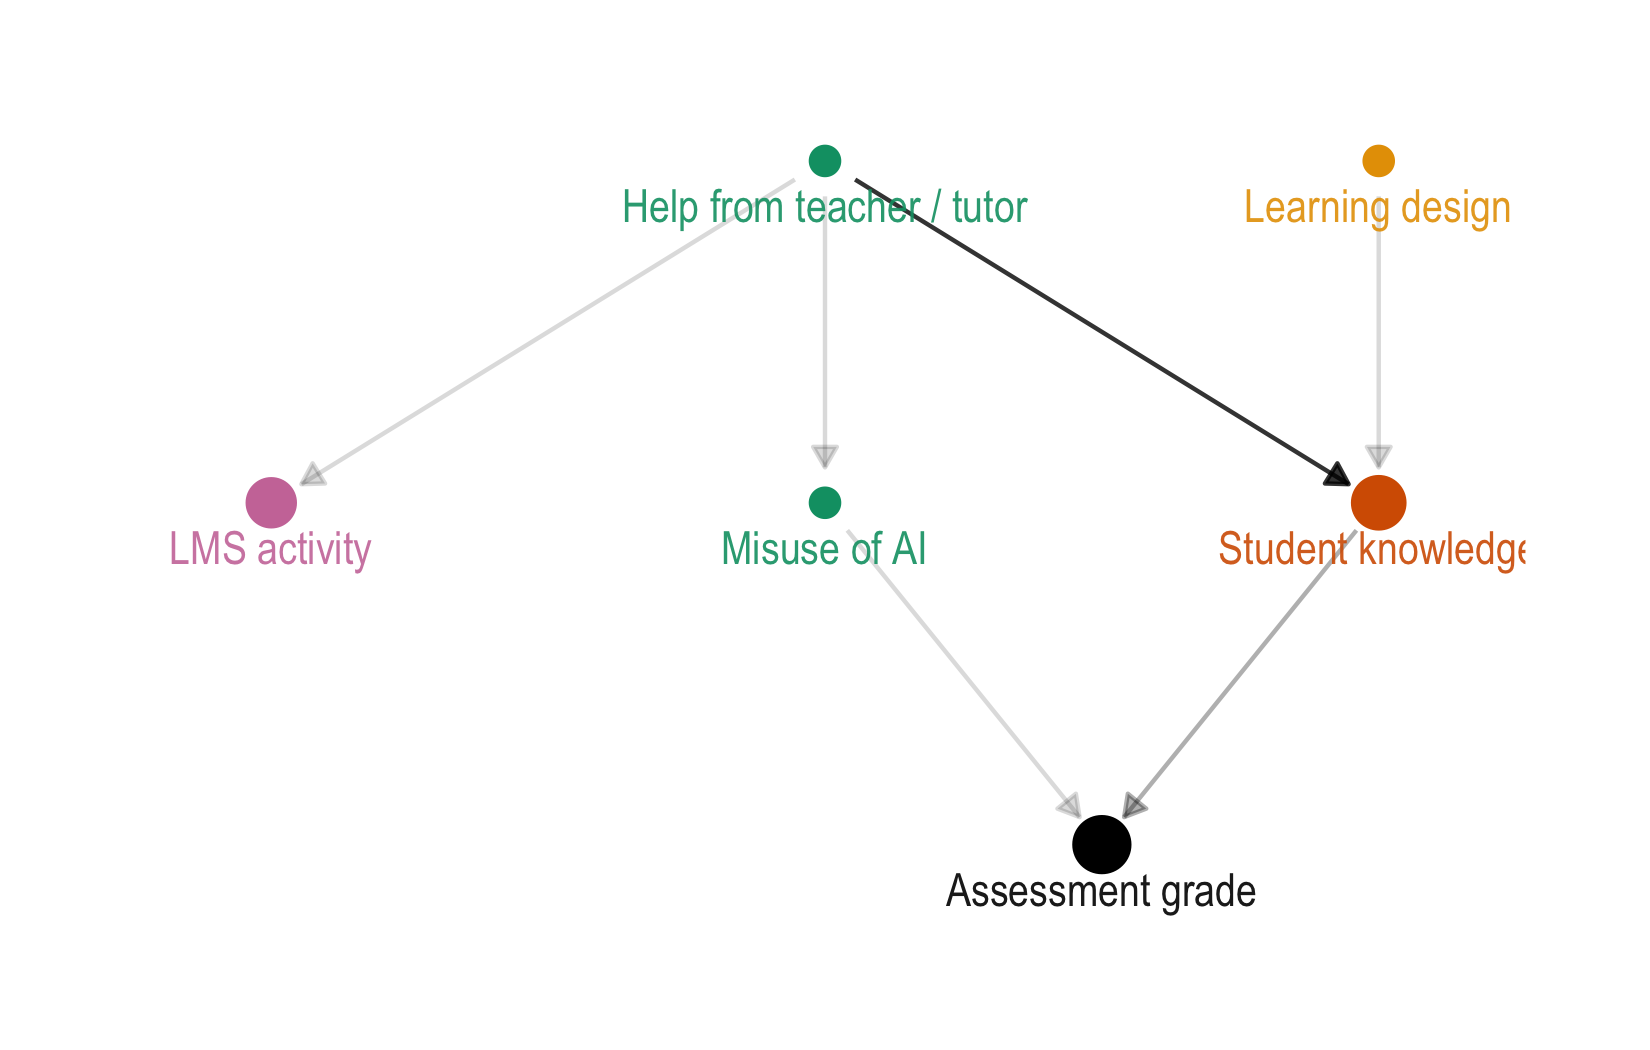
\includegraphics[keepaspectratio]{elicited-DAG-analysis_files/figure-pdf/unnamed-chunk-40-1.png}}

\begin{Shaded}
\begin{Highlighting}[]
\FunctionTok{ggsave}\NormalTok{(}\StringTok{"figures/FIG{-}{-}consensus{-}sub{-}model{-}filtered.jpg"}\NormalTok{, }
\NormalTok{       p\_top\_node\_groups\_filtered, }
       \AttributeTok{dpi =} \DecValTok{900}\NormalTok{, }
       \AttributeTok{height =} \DecValTok{4}\NormalTok{, }\AttributeTok{width =} \DecValTok{6}\NormalTok{)}
\end{Highlighting}
\end{Shaded}

All edges between node groups from the majority nodes

\begin{Shaded}
\begin{Highlighting}[]
\NormalTok{lyt\_coarse\_filtered\_ng\_full }\OtherTok{\textless{}{-}} \FunctionTok{create\_layout}\NormalTok{(}
\NormalTok{    coarse\_filtered\_graph\_ng\_filled, }
    \AttributeTok{layout =} \StringTok{"sugiyama"}\NormalTok{) }\SpecialCharTok{|\textgreater{}} 
    \FunctionTok{select}\NormalTok{(}\SpecialCharTok{{-}}\NormalTok{x, }\SpecialCharTok{{-}}\NormalTok{y) }\SpecialCharTok{|\textgreater{}} 
    \FunctionTok{inner\_join}\NormalTok{(lyt\_coarse\_filtered\_ng\_filtered }\SpecialCharTok{|\textgreater{}} \FunctionTok{select}\NormalTok{(x, y, node\_group))}
\end{Highlighting}
\end{Shaded}

\begin{verbatim}
Joining with `by = join_by(node_group)`
\end{verbatim}

\begin{Shaded}
\begin{Highlighting}[]
\NormalTok{p\_top\_node\_groups\_full }\OtherTok{\textless{}{-}} \FunctionTok{ggraph}\NormalTok{(lyt\_coarse\_filtered\_ng\_full) }\SpecialCharTok{+}
    \FunctionTok{geom\_edge\_fan}\NormalTok{(}\FunctionTok{aes}\NormalTok{(}\AttributeTok{edge\_linetype =} \FunctionTok{factor}\NormalTok{(switched), }\AttributeTok{alpha =}\NormalTok{ edge\_w, ), }\CommentTok{\# alpha = edge\_w, }
                  \AttributeTok{strength =} \FloatTok{0.8}\NormalTok{,}
                  \AttributeTok{arrow =} \FunctionTok{arrow}\NormalTok{(}\AttributeTok{length =} \FunctionTok{unit}\NormalTok{(}\DecValTok{2}\NormalTok{, }\StringTok{\textquotesingle{}mm\textquotesingle{}}\NormalTok{), }\AttributeTok{type =} \StringTok{"closed"}\NormalTok{),}
                  \AttributeTok{start\_cap =} \FunctionTok{circle}\NormalTok{(}\DecValTok{3}\NormalTok{, }\StringTok{\textquotesingle{}mm\textquotesingle{}}\NormalTok{),}
                  \AttributeTok{end\_cap =} \FunctionTok{circle}\NormalTok{(}\DecValTok{3}\NormalTok{, }\StringTok{\textquotesingle{}mm\textquotesingle{}}\NormalTok{)) }\SpecialCharTok{+}
    \FunctionTok{geom\_node\_point}\NormalTok{(}\FunctionTok{aes}\NormalTok{(}\AttributeTok{colour =}\NormalTok{ node\_type, }\AttributeTok{size =}\NormalTok{ node\_w)) }\SpecialCharTok{+}
    \FunctionTok{scale\_color\_okabe\_ito}\NormalTok{(}\AttributeTok{order =} \FunctionTok{c}\NormalTok{(}\DecValTok{9}\NormalTok{, }\DecValTok{7}\NormalTok{,}\DecValTok{1}\NormalTok{, }\DecValTok{2}\NormalTok{,}\DecValTok{3}\NormalTok{, }\DecValTok{6}\NormalTok{, }\DecValTok{8}\NormalTok{,}\DecValTok{5}\NormalTok{, }\DecValTok{4}\NormalTok{), }\AttributeTok{drop =} \ConstantTok{FALSE}\NormalTok{) }\SpecialCharTok{+}
        \CommentTok{\# ggsci::scale\_color\_npg(drop = FALSE) +}
        \CommentTok{\# geom\_node\_text(aes(label = name, size = node\_w, alpha = node\_w), nudge\_y = {-}.5) +}
        \FunctionTok{theme\_graph}\NormalTok{() }\SpecialCharTok{+}
        \FunctionTok{scale\_edge\_alpha\_continuous}\NormalTok{(}\AttributeTok{range =} \FunctionTok{c}\NormalTok{(}\FloatTok{0.15}\NormalTok{,}\FloatTok{0.8}\NormalTok{)) }\SpecialCharTok{+}
        \FunctionTok{scale\_alpha\_continuous}\NormalTok{(}\AttributeTok{range =} \FunctionTok{c}\NormalTok{(}\FloatTok{0.2}\NormalTok{,}\FloatTok{0.9}\NormalTok{)) }\SpecialCharTok{+}
        \FunctionTok{theme}\NormalTok{(}\AttributeTok{legend.position =} \StringTok{"none"}\NormalTok{) }\SpecialCharTok{+}
    \FunctionTok{scale\_size}\NormalTok{(}\AttributeTok{range =} \FunctionTok{c}\NormalTok{(}\DecValTok{3}\NormalTok{,}\DecValTok{6}\NormalTok{)) }\SpecialCharTok{+}
    \FunctionTok{geom\_node\_text}\NormalTok{(}\FunctionTok{aes}\NormalTok{(}\AttributeTok{label =}\NormalTok{ nice\_name, }\AttributeTok{colour =}\NormalTok{ node\_type), }
                   \AttributeTok{alpha =} \FloatTok{0.9}\NormalTok{, }\AttributeTok{nudge\_y =} \SpecialCharTok{{-}}\NormalTok{.}\DecValTok{13}\NormalTok{, }\AttributeTok{repel =}\NormalTok{ F) }\SpecialCharTok{+}
    \FunctionTok{xlim}\NormalTok{(}\FunctionTok{c}\NormalTok{(}
        \FunctionTok{min}\NormalTok{(lyt\_coarse\_filtered\_ng\_full}\SpecialCharTok{$}\NormalTok{x) }\SpecialCharTok{{-}} \FloatTok{0.15}\NormalTok{, }
        \FunctionTok{max}\NormalTok{(lyt\_coarse\_filtered\_ng\_full}\SpecialCharTok{$}\NormalTok{x) }\SpecialCharTok{+} \FloatTok{0.15}\NormalTok{))}

\NormalTok{p\_top\_node\_groups\_full}
\end{Highlighting}
\end{Shaded}

\pandocbounded{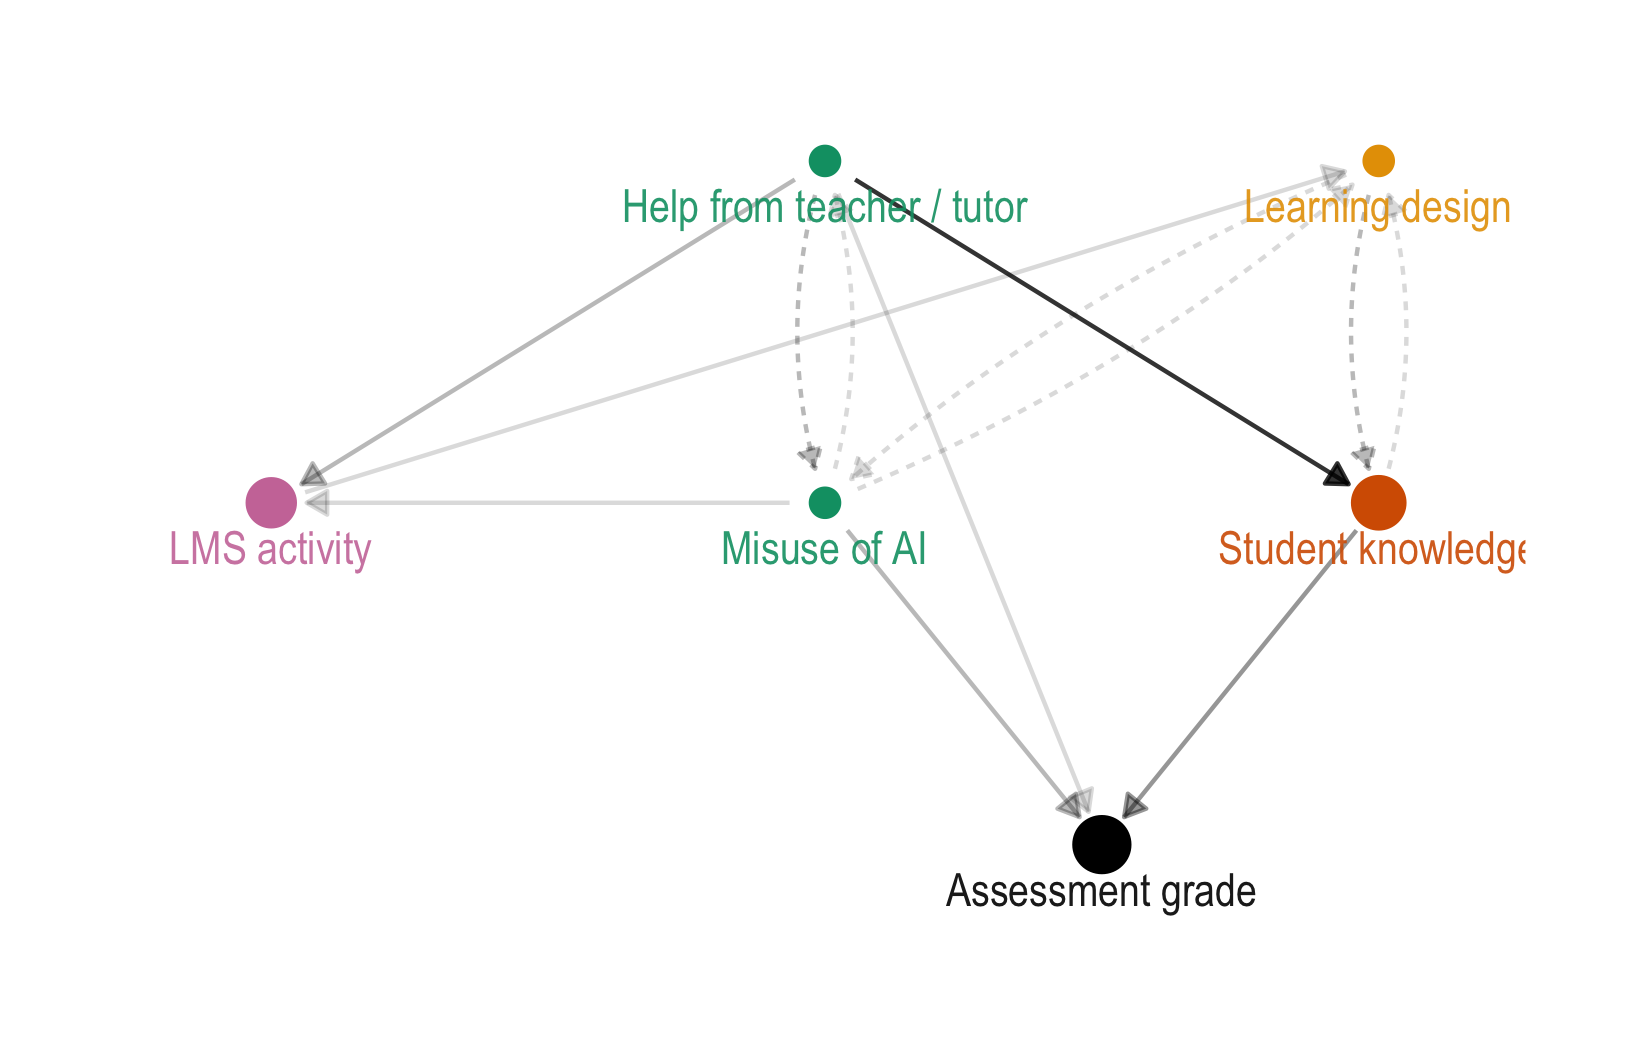
\includegraphics[keepaspectratio]{elicited-DAG-analysis_files/figure-pdf/unnamed-chunk-41-1.png}}

\begin{Shaded}
\begin{Highlighting}[]
\FunctionTok{ggsave}\NormalTok{(}\StringTok{"figures/FIG{-}{-}consensus{-}sub{-}model{-}full.jpg"}\NormalTok{,}
\NormalTok{       p\_top\_node\_groups\_full,}
       \AttributeTok{dpi =} \DecValTok{900}\NormalTok{,}
       \AttributeTok{height =} \DecValTok{4}\NormalTok{, }\AttributeTok{width =} \DecValTok{6}\NormalTok{)}
\end{Highlighting}
\end{Shaded}

Node groups close to the constructs: - Belonging - Mindset -
Collaboration

\begin{Shaded}
\begin{Highlighting}[]
\CommentTok{\# all nodes}
\NormalTok{all\_nodes\_with\_metrics }\SpecialCharTok{|\textgreater{}} 
    \FunctionTok{inner\_join}\NormalTok{(name\_node\_nice\_name) }\SpecialCharTok{|\textgreater{}} 
    \FunctionTok{inner\_join}\NormalTok{(node\_group\_nice\_name }\SpecialCharTok{|\textgreater{}} \FunctionTok{rename}\NormalTok{(}\AttributeTok{g\_nice\_name =}\NormalTok{ nice\_name)) }\SpecialCharTok{|\textgreater{}} 
    \FunctionTok{select}\NormalTok{(name, nice\_name, g\_nice\_name, node\_group, Model, pagerank\_no\_outcome, pagerank, btw\_rel\_rank) }\SpecialCharTok{|\textgreater{}} 
    \FunctionTok{arrange}\NormalTok{(name, Model) }\SpecialCharTok{|\textgreater{}} 
\NormalTok{    knitr}\SpecialCharTok{::}\FunctionTok{kable}\NormalTok{()}
\end{Highlighting}
\end{Shaded}

\begin{verbatim}
Joining with `by = join_by(name)`
Joining with `by = join_by(node_group)`
\end{verbatim}

\begin{longtable}[]{@{}
  >{\raggedright\arraybackslash}p{(\linewidth - 14\tabcolsep) * \real{0.1053}}
  >{\raggedright\arraybackslash}p{(\linewidth - 14\tabcolsep) * \real{0.2895}}
  >{\raggedright\arraybackslash}p{(\linewidth - 14\tabcolsep) * \real{0.1908}}
  >{\raggedright\arraybackslash}p{(\linewidth - 14\tabcolsep) * \real{0.0921}}
  >{\raggedright\arraybackslash}p{(\linewidth - 14\tabcolsep) * \real{0.0395}}
  >{\raggedleft\arraybackslash}p{(\linewidth - 14\tabcolsep) * \real{0.1316}}
  >{\raggedleft\arraybackslash}p{(\linewidth - 14\tabcolsep) * \real{0.0658}}
  >{\raggedleft\arraybackslash}p{(\linewidth - 14\tabcolsep) * \real{0.0855}}@{}}
\toprule\noalign{}
\begin{minipage}[b]{\linewidth}\raggedright
name
\end{minipage} & \begin{minipage}[b]{\linewidth}\raggedright
nice\_name
\end{minipage} & \begin{minipage}[b]{\linewidth}\raggedright
g\_nice\_name
\end{minipage} & \begin{minipage}[b]{\linewidth}\raggedright
node\_group
\end{minipage} & \begin{minipage}[b]{\linewidth}\raggedright
Model
\end{minipage} & \begin{minipage}[b]{\linewidth}\raggedleft
pagerank\_no\_outcome
\end{minipage} & \begin{minipage}[b]{\linewidth}\raggedleft
pagerank
\end{minipage} & \begin{minipage}[b]{\linewidth}\raggedleft
btw\_rel\_rank
\end{minipage} \\
\midrule\noalign{}
\endhead
\bottomrule\noalign{}
\endlastfoot
CD & Any system data & Course Data & CD.Str & S1 & 0.2598017 & 0.1254606
& 0.5000000 \\
CD.Att & Attendance & Student attendance & CD.Att & S4 & 0.0229468 &
0.0435213 & 0.5333333 \\
CD.Att & Attendance & Student attendance & CD.Att & S7 & 0.0348776 &
0.0360250 & 0.6500000 \\
CD.LMS & LMS activity & LMS activity & CD.LMS & S2 & 0.0489246 &
0.0601186 & 0.7272727 \\
CD.LMS & LMS activity & LMS activity & CD.LMS & S3 & 0.1242479 &
0.0777349 & 0.4000000 \\
CD.LMS & LMS activity & LMS activity & CD.LMS & S4 & 0.1161226 &
0.0715014 & 0.5333333 \\
CD.LMS & LMS activity & LMS activity & CD.LMS & S6 & 0.0633664 &
0.0518777 & 0.8461538 \\
CD.LMS & LMS activity & LMS activity & CD.LMS & S7 & 0.0403759 &
0.0398677 & 0.6500000 \\
CD.LMS & LMS activity & LMS activity & CD.LMS & S8 & 0.0576999 &
0.0576577 & 0.1428571 \\
CD.LMS.code & Code artifacts & LMS activity & CD.LMS & S7 & 0.0415103 &
0.0399127 & 0.6500000 \\
CD.LMS.write & Writing artifacts & LMS activity & CD.LMS & S7 &
0.0752913 & 0.0477832 & 0.6500000 \\
CD.Str & Course Data & Course Data & CD.Str & S2 & 0.0693898 & 0.0754642
& 0.7272727 \\
CD.Str & Course Data & Course Data & CD.Str & S3 & 0.0569482 & 0.0657501
& 0.4000000 \\
CD.Str & Course Data & Course Data & CD.Str & S6 & 0.0276203 & 0.0375671
& 0.8461538 \\
Grade & Assessment grade & Assessment grade & Grade.Outcome & S1 &
0.0000000 & 0.1323841 & 0.5000000 \\
Grade & Assessment grade & Assessment grade & Grade.Outcome & S2 &
0.0000000 & 0.1642797 & 0.7272727 \\
Grade & Assessment grade & Assessment grade & Grade.Outcome & S3 &
0.0000000 & 0.0732885 & 0.4000000 \\
Grade & Assessment grade & Assessment grade & Grade.Outcome & S4 &
0.0000000 & 0.0787048 & 0.5333333 \\
Grade & Assessment grade & Assessment grade & Grade.Outcome & S5 &
0.0000000 & 0.1730290 & 0.5294118 \\
Grade & Assessment grade & Assessment grade & Grade.Outcome & S6 &
0.0000000 & 0.1439293 & 0.0769231 \\
Grade & Assessment grade & Assessment grade & Grade.Outcome & S7 &
0.0000000 & 0.1275476 & 0.6500000 \\
Grade & Assessment grade & Assessment grade & Grade.Outcome & S8 &
0.0000000 & 0.1531532 & 0.7142857 \\
Grade.Coms & Mark - Communication & Preliminary assessments &
Assessments & S7 & 0.0562769 & 0.0477944 & 0.5500000 \\
Grade.Exam & Mark - Exam & Preliminary assessments & Assessments & S5 &
0.1621565 & 0.0893094 & 0.2941176 \\
Grade.Interp & Mark - Interpretation & Preliminary assessments &
Assessments & S7 & 0.1158678 & 0.0708185 & 0.5500000 \\
Grade.Proc & Mark - Learning process & Preliminary assessments &
Assessments & S5 & 0.0762812 & 0.0573829 & 0.3529412 \\
Grade.Quiz & Mark - Quiz & Preliminary assessments & Assessments & S5 &
0.0520260 & 0.0453547 & 0.4117647 \\
Grade.Ref & Mark - Learning reflection & Preliminary assessments &
Assessments & S5 & 0.1193653 & 0.0888427 & 0.2352941 \\
Grade.Tech & Mark - Technical & Preliminary assessments & Assessments &
S7 & 0.0681343 & 0.0531444 & 0.4500000 \\
H & Help (general) & Help from teacher / tutor & H.Tut & S1 & 0.0534232
& 0.0643216 & 0.3000000 \\
H & Help (general) & Help from teacher / tutor & H.Tut & S6 & 0.0695564
& 0.0633944 & 0.3846154 \\
H & Help (general) & Help from teacher / tutor & H.Tut & S8 & 0.0709553
& 0.0672673 & 0.0000000 \\
H.AI & Help from AI (any) & Help from AI & H.AI.good & S3 & 0.0202678 &
0.0380242 & 0.4000000 \\
H.AI & Help from AI (any) & Help from AI & H.AI.good & S4 & 0.0330791 &
0.0559560 & 0.2000000 \\
H.AI.Agent & Help from AI (agent) & Help from AI & H.AI.good & S5 &
0.0293150 & 0.0325841 & 0.5294118 \\
H.AI.Agent & Help from AI (agent) & Help from AI & H.AI.good & S8 &
0.0311891 & 0.0384384 & 0.7142857 \\
H.AI.Fb & Help from AI (feedback) & Help from AI & H.AI.good & S5 &
0.0293150 & 0.0325841 & 0.5294118 \\
H.AI.Fb & Help from AI (feedback) & Help from AI & H.AI.good & S7 &
0.0367908 & 0.0366855 & 0.1500000 \\
H.AI.Res & Help from AI (research) & Help from AI & H.AI.good & S5 &
0.0293150 & 0.0325841 & 0.5294118 \\
H.AI.Study & Help from AI (revision) & Help from AI & H.AI.good & S5 &
0.0293150 & 0.0325841 & 0.5294118 \\
H.AI.Study & Help from AI (revision) & Help from AI & H.AI.good & S7 &
0.0367908 & 0.0366855 & 0.4000000 \\
H.AI.evil & Misuse of AI & Misuse of AI & H.AI.evil & S2 & 0.2333173 &
0.0929255 & 0.6363636 \\
H.AI.evil & Misuse of AI & Misuse of AI & H.AI.evil & S5 & 0.0293150 &
0.0325841 & 0.5294118 \\
H.AI.evil & Misuse of AI & Misuse of AI & H.AI.evil & S6 & 0.1136701 &
0.0678082 & 0.6923077 \\
H.AI.evil & Misuse of AI & Misuse of AI & H.AI.evil & S8 & 0.0311891 &
0.0384384 & 0.7142857 \\
H.AI.evil.code & Misuse of AI (code) & Misuse of AI & H.AI.evil & S7 &
0.0367908 & 0.0366855 & 0.1000000 \\
H.AI.evil.write & Misuse from AI (write) & Misuse of AI & H.AI.evil & S7
& 0.0367908 & 0.0366855 & 0.0500000 \\
H.AI.good & Help from AI (to learn) & Help from AI & H.AI.good & S2 &
0.0477452 & 0.0595770 & 0.2727273 \\
H.AI.good & Help from AI (to learn) & Help from AI & H.AI.good & S6 &
0.0841086 & 0.0572424 & 0.3846154 \\
H.Ment & Help from mentor & Help from teacher / tutor & H.Tut & S5 &
0.0293150 & 0.0325841 & 0.5294118 \\
H.Peer & Help from peers & Help from peers & H.Peer & S2 & 0.0477452 &
0.0595770 & 0.4545455 \\
H.Peer & Help from peers & Help from peers & H.Peer & S3 & 0.0202678 &
0.0380242 & 0.4000000 \\
H.Peer & Help from peers & Help from peers & H.Peer & S4 & 0.0287095 &
0.0489615 & 0.3333333 \\
H.Tut & Help from teacher / tutor & Help from teacher / tutor & H.Tut &
S3 & 0.2051369 & 0.0891319 & 0.1333333 \\
H.Tut & Help from teacher / tutor & Help from teacher / tutor & H.Tut &
S4 & 0.0287095 & 0.0489615 & 0.4000000 \\
H.Tut & Help from teacher / tutor & Help from teacher / tutor & H.Tut &
S5 & 0.0293150 & 0.0325841 & 0.5294118 \\
H.Tut & Help from teacher / tutor & Help from teacher / tutor & H.Tut &
S8 & 0.0311891 & 0.0384384 & 0.7142857 \\
H.Tut.Fb & Feedback from teacher / tutor & Help from teacher / tutor &
H.Tut & S2 & 0.0489246 & 0.0601186 & 0.3636364 \\
H.other.evil & Cheating - non-AI & Cheating - non-AI & H.Cheat & S7 &
0.0458741 & 0.0437103 & 0.2000000 \\
LD & Learning design & Learning design & LD & S2 & 0.0408079 & 0.0541609
& 0.7272727 \\
LD.AIguide & Guidance on AI use & Learning design & LD & S6 & 0.0276203
& 0.0375671 & 0.8461538 \\
LD.Task & Task design & Learning design & LD & S1 & 0.1516042 &
0.1313233 & 0.0000000 \\
LD.Task & Task design & Learning design & LD & S3 & 0.0863070 &
0.1109038 & 0.0666667 \\
LD.Task & Task design & Learning design & LD & S6 & 0.0510975 &
0.0563506 & 0.5384615 \\
LD.Task & Task design & Learning design & LD & S8 & 0.0444445 &
0.0480480 & 0.2857143 \\
LD.Task.Code & Coding task design & Learning design & LD & S8 &
0.0601301 & 0.0560561 & 0.3571429 \\
LD.Task.Grp & Groupwork task design & Learning design & LD & S8 &
0.1845208 & 0.1225225 & 0.0714286 \\
LD.Task.Other & Other task design & Learning design & LD & S8 &
0.0311891 & 0.0384384 & 0.7142857 \\
LD.Task.Prac & Practical task design & Learning design & LD & S8 &
0.0601301 & 0.0560561 & 0.3571429 \\
LD.Task.Write & Writing task design & Learning design & LD & S8 &
0.0601301 & 0.0560561 & 0.3571429 \\
S.Act & Student decisions / actions & Student decisions / actions &
S.Act & S2 & 0.0477452 & 0.0595770 & 0.1818182 \\
S.Act & Student decisions / actions & Student decisions / actions &
S.Act & S3 & 0.0260103 & 0.0443615 & 0.3333333 \\
S.Act & Student decisions / actions & Student decisions / actions &
S.Act & S6 & 0.1533177 & 0.0965383 & 0.0000000 \\
S.Act.AIstrat & Student AI strategy & Student decisions / actions &
S.Act & S7 & 0.0513724 & 0.0475530 & 0.0000000 \\
S.Act.Fb & Student acts on feedback & Student decisions / actions &
S.Act & S4 & 0.1870171 & 0.0908156 & 0.2666667 \\
S.Act.Fb & Student acts on feedback & Student decisions / actions &
S.Act & S6 & 0.1579403 & 0.0617016 & 0.3076923 \\
S.Act.Fb.Post & Student acts on feedback between subjects & Student
decisions / actions & S.Act & S6 & 0.0276203 & 0.1095317 & 0.2307692 \\
S.Act.Frm & Student does formative tasks & Student decisions / actions &
S.Act & S4 & 0.2311575 & 0.1367896 & 0.0000000 \\
S.Act.Perf & Student performance on task & Student decisions / actions &
S.Act & S3 & 0.2006032 & 0.1410574 & 0.0000000 \\
S.Act.Time & Student commits time & Student decisions / actions & S.Act
& S7 & 0.0423690 & 0.0422693 & 0.2500000 \\
S.Aff.Integ & Student acting with integrity & Student emotion /
motivation & S.EM & S1 & 0.0440604 & 0.0571748 & 0.5000000 \\
S.Aff.Joy & Student enjoyment & Student emotion / motivation & S.EM & S5
& 0.0417738 & 0.0407302 & 0.4705882 \\
S.Aff.MindSet & Student mindset & Student emotion / motivation & S.EM &
S4 & 0.0178806 & 0.0373040 & 0.5333333 \\
S.Aff.MindSet & Student mindset & Student emotion / motivation & S.EM &
S5 & 0.0719866 & 0.0590588 & 0.0000000 \\
S.Aff.MindSet & Student mindset & Student emotion / motivation & S.EM &
S7 & 0.0258742 & 0.0307413 & 0.6500000 \\
S.Aff.Safe & Student feels safe & Student emotion / motivation & S.EM &
S5 & 0.0355444 & 0.0366572 & 0.5294118 \\
S.Aff.WrkLd & Student workload pressure & Student emotion / motivation &
S.EM & S1 & 0.0820852 & 0.0795087 & 0.3000000 \\
S.Aff.WrkLd & Student workload pressure & Student emotion / motivation &
S.EM & S4 & 0.0178806 & 0.0373040 & 0.5333333 \\
S.Aff.WrkLd & Student workload pressure & Student emotion / motivation &
S.EM & S7 & 0.0258742 & 0.0307413 & 0.6500000 \\
S.Att.Eq & Student equity group & Student attributes & S.Att & S6 &
0.0493367 & 0.0516547 & 0.6153846 \\
S.Att.HSk & Student seeks help & Student attributes & S.Att & S4 &
0.0254798 & 0.0466300 & 0.4666667 \\
S.Att.Nro & Student neuro-divergent & Student attributes & S.Att & S4 &
0.0178806 & 0.0373040 & 0.5333333 \\
S.Att.SocCap & Student social capital & Student attributes & S.Att & S1
& 0.0440604 & 0.0571748 & 0.5000000 \\
S.Cp.Aca & Student academic skill & Student metacognitive skill & S.Cp &
S3 & 0.0260103 & 0.0443615 & 0.2666667 \\
S.Cp.Aca & Student academic skill & Student metacognitive skill & S.Cp &
S5 & 0.0570710 & 0.0481125 & 0.1176471 \\
S.Cp.Aca & Student academic skill & Student metacognitive skill & S.Cp &
S6 & 0.0689204 & 0.0755157 & 0.7692308 \\
S.Cp.EvJdg & Student evaluative judgement & Student metacognitive skill
& S.Cp & S4 & 0.0178806 & 0.0373040 & 0.5333333 \\
S.Cp.Fb & Student feedback literacy & Student metacognitive skill & S.Cp
& S4 & 0.0754671 & 0.0819911 & 0.0666667 \\
S.Cp.Grp & Student groupwork capability & Student metacognitive skill &
S.Cp & S8 & 0.2169727 & 0.1173173 & 0.2142857 \\
S.Cp.Ind & Student individual work capability & Student metacognitive
skill & S.Cp & S8 & 0.0601301 & 0.0560561 & 0.5714286 \\
S.Cp.Lrn & Student metacognative learning capabilities & Student
metacognitive skill & S.Cp & S5 & 0.1277487 & 0.0893942 & 0.0588235 \\
S.Cp.SRL & Student SRL & Student metacognitive skill & S.Cp & S2 &
0.2101735 & 0.1149792 & 0.0909091 \\
S.Kn & Student subject knowledge & Student knowledge & S.Kn & S1 &
0.0894701 & 0.0893356 & 0.2000000 \\
S.Kn & Student subject knowledge & Student knowledge & S.Kn & S2 &
0.1574813 & 0.1396450 & 0.0000000 \\
S.Kn & Student subject knowledge & Student knowledge & S.Kn & S3 &
0.1328617 & 0.0872409 & 0.2000000 \\
S.Kn & Student subject knowledge & Student knowledge & S.Kn & S4 &
0.1619080 & 0.1096473 & 0.1333333 \\
S.Kn & Student subject knowledge & Student knowledge & S.Kn & S5 &
0.0508416 & 0.0440395 & 0.1764706 \\
S.Kn & Student subject knowledge & Student knowledge & S.Kn & S6 &
0.1058251 & 0.0893212 & 0.1538462 \\
S.Kn & Student subject knowledge & Student knowledge & S.Kn & S8 &
0.0601301 & 0.0560561 & 0.5714286 \\
S.Kn.Coms & Student communications knowledge & Student knowledge & S.Kn
& S7 & 0.0470086 & 0.0437554 & 0.5000000 \\
S.Kn.Interp & Student interpretation knowledge & Student knowledge &
S.Kn & S7 & 0.0936112 & 0.0679259 & 0.2500000 \\
S.Kn.Prior & Student prior knowledge & Student prior knowledge &
S.Kn.Prior & S4 & 0.0178806 & 0.0373040 & 0.5333333 \\
S.Kn.Prior & Student prior knowledge & Student prior knowledge &
S.Kn.Prior & S7 & 0.0258742 & 0.0307413 & 0.6500000 \\
S.Kn.Tech & Student technical knowledge & Student knowledge & S.Kn & S7
& 0.0626447 & 0.0529267 & 0.3500000 \\
T.Act.UseAI & Teacher use of AI & Teacher use of AI & T.Act & S3 &
0.0202678 & 0.0380242 & 0.4000000 \\
T.Aff.Integ & Teacher acts with integrity & Teacher emotion / motivation
& T.EM & S1 & 0.0534232 & 0.0643216 & 0.5000000 \\
T.Aff.WrkLd & Teacher workload pressure & Teacher emotion / motivation &
T.EM & S1 & 0.0440604 & 0.0571748 & 0.5000000 \\
T.Cp.Inst & Teacher instruction quality & Teacher capabilities & T.Cp &
S2 & 0.0477452 & 0.0595770 & 0.4545455 \\
T.Cp.KnStu & Teacher knows students & Teacher capabilities & T.Cp & S3 &
0.0202678 & 0.0380242 & 0.4000000 \\
T.Cp.Mark & Teacher reliably marks & Teacher capabilities & T.Cp & S1 &
0.1780112 & 0.1418202 & 0.1000000 \\
T.Kn.AI & Teacher AI literacy & Teacher knowledge & T.Kn & S3 &
0.0202678 & 0.0380242 & 0.4000000 \\
T.Kn.Ass & Teacher assessment literacy & Teacher knowledge & T.Kn & S3 &
0.0202678 & 0.0380242 & 0.4000000 \\
T.Kn.Sub & Teacher subject knowledge & Teacher knowledge & T.Kn & S3 &
0.0202678 & 0.0380242 & 0.4000000 \\
\end{longtable}

\subsection{Node importance and
measurability}\label{node-importance-and-measurability}

\begin{Shaded}
\begin{Highlighting}[]
\NormalTok{all\_node\_groups\_aggregated\_metrics }\OtherTok{\textless{}{-}} 
\NormalTok{    all\_nodes\_with\_metrics }\SpecialCharTok{|\textgreater{}} 
    \FunctionTok{group\_by}\NormalTok{(Model, node\_group, node\_type) }\SpecialCharTok{|\textgreater{}} 
    \FunctionTok{summarise}\NormalTok{(}
        \AttributeTok{p\_traced =} \FunctionTok{mean}\NormalTok{(measurability }\SpecialCharTok{==} \StringTok{"DW"}\NormalTok{),}
        \AttributeTok{measurability =}\NormalTok{ (}\DecValTok{3} \SpecialCharTok{*} \FunctionTok{mean}\NormalTok{(measurability }\SpecialCharTok{==} \StringTok{"DW"}\NormalTok{) }\SpecialCharTok{+}
                             \DecValTok{2} \SpecialCharTok{*} \FunctionTok{mean}\NormalTok{(measurability }\SpecialCharTok{==} \StringTok{"O"}\NormalTok{) }\SpecialCharTok{+}
                             \FunctionTok{mean}\NormalTok{(measurability }\SpecialCharTok{==} \StringTok{"PO"}\NormalTok{)) }\SpecialCharTok{/} \DecValTok{3}\NormalTok{,}
        \AttributeTok{pagerank =} \FunctionTok{sum}\NormalTok{(pagerank),}
              \AttributeTok{pagerank\_no\_outcome =} \FunctionTok{sum}\NormalTok{(pagerank\_no\_outcome),}
              \AttributeTok{btw\_rel =} \FunctionTok{sum}\NormalTok{(btw\_rel)) }\SpecialCharTok{|\textgreater{}} 
    \FunctionTok{group\_by}\NormalTok{(node\_group, node\_type) }\SpecialCharTok{|\textgreater{}} 
    \FunctionTok{mutate}\NormalTok{(}
        \AttributeTok{n =} \FunctionTok{n}\NormalTok{(),}
        \AttributeTok{overall\_pagerank =} \FunctionTok{sum}\NormalTok{(pagerank }\SpecialCharTok{/} \DecValTok{8}\NormalTok{),}
           \AttributeTok{overall\_pagerank\_no\_outcome =} \FunctionTok{sum}\NormalTok{(pagerank\_no\_outcome }\SpecialCharTok{/} \DecValTok{8}\NormalTok{),}
           \AttributeTok{overall\_btw =} \FunctionTok{sum}\NormalTok{(btw\_rel)) }\SpecialCharTok{|\textgreater{}} 
    \FunctionTok{ungroup}\NormalTok{()}
\end{Highlighting}
\end{Shaded}

\begin{verbatim}
`summarise()` has grouped output by 'Model', 'node_group'. You can override
using the `.groups` argument.
\end{verbatim}

\paragraph{Figure: Node importance and data
availability}\label{figure-node-importance-and-data-availability}

\begin{Shaded}
\begin{Highlighting}[]
\NormalTok{d\_ng\_measurability\_importance }\OtherTok{\textless{}{-}} 
\NormalTok{    all\_node\_groups\_aggregated\_metrics }\SpecialCharTok{|\textgreater{}} 
    \FunctionTok{filter}\NormalTok{(node\_group }\SpecialCharTok{!=} \StringTok{"Grade.Outcome"}\NormalTok{) }\SpecialCharTok{|\textgreater{}}
    \FunctionTok{inner\_join}\NormalTok{(node\_group\_nice\_name, }\AttributeTok{by =} \StringTok{"node\_group"}\NormalTok{) }\SpecialCharTok{|\textgreater{}}
    \FunctionTok{mutate}\NormalTok{(}\AttributeTok{node\_group =}\NormalTok{ nice\_name) }\SpecialCharTok{|\textgreater{}}
    \FunctionTok{group\_by}\NormalTok{(node\_group) }\SpecialCharTok{|\textgreater{}}
    \FunctionTok{mutate}\NormalTok{(}\AttributeTok{m\_group =} \FunctionTok{mean}\NormalTok{(measurability)) }\SpecialCharTok{|\textgreater{}}
    \FunctionTok{ungroup}\NormalTok{() }\SpecialCharTok{|\textgreater{}} 
    \FunctionTok{mutate}\NormalTok{(}\AttributeTok{node\_group =} \FunctionTok{fct\_reorder}\NormalTok{(node\_group, pagerank\_no\_outcome)) }\SpecialCharTok{|\textgreater{}} 
    \FunctionTok{arrange}\NormalTok{(}\FunctionTok{desc}\NormalTok{(node\_group)) }\SpecialCharTok{|\textgreater{}} 
    \FunctionTok{filter}\NormalTok{(n }\SpecialCharTok{\textgreater{}} \DecValTok{3}\NormalTok{) }\CommentTok{\# need at least half the models with node group}


\NormalTok{p\_top\_node\_pagerank\_no\_outcome\_measurability }\OtherTok{\textless{}{-}} 
\NormalTok{    d\_ng\_measurability\_importance }\SpecialCharTok{|\textgreater{}} 
    \CommentTok{\# arrange(Model, node\_group) |\textgreater{} }
    \FunctionTok{ggplot}\NormalTok{(}\FunctionTok{aes}\NormalTok{(}\AttributeTok{x =}\NormalTok{ pagerank\_no\_outcome, }\AttributeTok{y =}\NormalTok{ node\_group)) }\SpecialCharTok{+}
    \FunctionTok{geom\_boxplot}\NormalTok{(}\FunctionTok{aes}\NormalTok{(}\AttributeTok{fill =}\NormalTok{ m\_group), }\AttributeTok{colour =} \StringTok{"lightgray"}\NormalTok{, }\AttributeTok{size =} \FloatTok{0.4}\NormalTok{, }\AttributeTok{alpha =} \FloatTok{0.7}\NormalTok{) }\SpecialCharTok{+}
    \CommentTok{\# geom\_line(aes(x = pagerank\_no\_outcome, y = node\_group, group = Model), alpha = 0.6) +}
    \FunctionTok{geom\_point}\NormalTok{(}\FunctionTok{aes}\NormalTok{(}\AttributeTok{colour =}\NormalTok{ measurability), }\AttributeTok{alpha =} \FloatTok{0.9}\NormalTok{) }\SpecialCharTok{+}
    \FunctionTok{scale\_color\_gradient}\NormalTok{(}
        \AttributeTok{low =} \StringTok{"darkslateblue"}\NormalTok{, }
        \CommentTok{\# mid = "darkturquoise",}
        \AttributeTok{high =} \StringTok{"aquamarine"}\NormalTok{,}
        \CommentTok{\# midpoint = mean(range(d\_ng\_measurability\_importance$measurability)),}
        \AttributeTok{limits =} \FunctionTok{c}\NormalTok{(}\DecValTok{0}\NormalTok{,}\DecValTok{1}\NormalTok{),}
        \AttributeTok{breaks =} \FunctionTok{c}\NormalTok{(}\DecValTok{0}\NormalTok{, }\DecValTok{1}\SpecialCharTok{/}\DecValTok{3}\NormalTok{, }\DecValTok{2}\SpecialCharTok{/}\DecValTok{3}\NormalTok{, }\DecValTok{1}\NormalTok{),}
        \AttributeTok{labels =} \FunctionTok{c}\NormalTok{(}\StringTok{"Latent"}\NormalTok{,}\StringTok{"Potentially}\SpecialCharTok{\textbackslash{}n}\StringTok{observable"}\NormalTok{, }\StringTok{"Observable"}\NormalTok{, }\StringTok{"Data}\SpecialCharTok{\textbackslash{}n}\StringTok{Warehouse"}\NormalTok{),}
        \AttributeTok{name =} \StringTok{""}\NormalTok{,}
        \AttributeTok{guide =} \FunctionTok{guide\_colorbar}\NormalTok{(}\AttributeTok{reverse =} \ConstantTok{FALSE}\NormalTok{)}
\NormalTok{    ) }\SpecialCharTok{+}
    \FunctionTok{scale\_fill\_gradient}\NormalTok{(}
        \CommentTok{\# midpoint = mean(range(d\_ng\_measurability\_importance$m\_group)),}
        \AttributeTok{limits =} \FunctionTok{c}\NormalTok{(}\DecValTok{0}\NormalTok{,}\DecValTok{1}\NormalTok{),}
                \AttributeTok{low =} \StringTok{"darkslateblue"}\NormalTok{, }
        \CommentTok{\# mid = "darkturquoise",}
        \AttributeTok{high =} \StringTok{"aquamarine"}
\NormalTok{        ) }\SpecialCharTok{+}
    \FunctionTok{theme\_minimal}\NormalTok{() }\SpecialCharTok{+}
    \FunctionTok{ylab}\NormalTok{(}\StringTok{"Node group"}\NormalTok{) }\SpecialCharTok{+}
    \FunctionTok{xlab}\NormalTok{(}\StringTok{"Node groups combined Centrality (Pagerank)"}\NormalTok{) }\SpecialCharTok{+}
    \CommentTok{\# geom\_rug(aes(colour = m\_dist\_to\_trace), alpha = 0.6, sides = "b") +}
    \CommentTok{\# coord\_cartesian(clip = "off") +}
    \FunctionTok{guides}\NormalTok{(}\AttributeTok{fill =} \StringTok{"none"}\NormalTok{) }\SpecialCharTok{+}
    \FunctionTok{theme}\NormalTok{(}\AttributeTok{legend.position =} \StringTok{"bottom"}\NormalTok{,}
          \AttributeTok{legend.justification =} \StringTok{"center"}\NormalTok{,}
    \AttributeTok{legend.box.just =} \StringTok{"center"}\NormalTok{,}
          \AttributeTok{legend.text  =} \FunctionTok{element\_text}\NormalTok{(}\AttributeTok{size =} \DecValTok{8}\NormalTok{),}
          \AttributeTok{legend.key.width =} \FunctionTok{unit}\NormalTok{(}\DecValTok{1}\NormalTok{, }\StringTok{"cm"}\NormalTok{),}
          \AttributeTok{axis.ticks.y =} \FunctionTok{element\_blank}\NormalTok{(),}
          \AttributeTok{axis.line.y =} \FunctionTok{element\_blank}\NormalTok{(),}
          \AttributeTok{panel.grid.major.y =} \FunctionTok{element\_blank}\NormalTok{(),}
          \AttributeTok{panel.grid.minor.y =} \FunctionTok{element\_blank}\NormalTok{())}

\CommentTok{\# p\_top\_node\_pagerank\_no\_outcome\_measurability}

\CommentTok{\# extract legend}
\NormalTok{leg }\OtherTok{\textless{}{-}} \FunctionTok{get\_legend}\NormalTok{(p\_top\_node\_pagerank\_no\_outcome\_measurability)}

\CommentTok{\# arrange with relative heights (legend gets a small slice)}
\NormalTok{p\_node\_importance\_with\_measurability }\OtherTok{\textless{}{-}}\NormalTok{ (}\FunctionTok{wrap\_elements}\NormalTok{(leg) }\SpecialCharTok{/}
\NormalTok{    (p\_top\_node\_pagerank\_no\_outcome\_measurability }\SpecialCharTok{+} \FunctionTok{theme}\NormalTok{(}\AttributeTok{legend.position =} \StringTok{"none"}\NormalTok{))) }\SpecialCharTok{+}
  \FunctionTok{plot\_layout}\NormalTok{(}\AttributeTok{heights =} \FunctionTok{c}\NormalTok{(}\FloatTok{0.2}\NormalTok{, }\DecValTok{1}\NormalTok{))}

\CommentTok{\# p\_node\_importance\_with\_measurability}
\CommentTok{\# ggsave("figures/FIG{-}{-}node\_pagerank\_no\_outcome\_measurability.png", p\_node\_importance\_with\_measurability,}
\CommentTok{\#        width = 5,}
\CommentTok{\#        height = 4,}
\CommentTok{\#        dpi = 900)}
\end{Highlighting}
\end{Shaded}

With discrete scale instead

\begin{Shaded}
\begin{Highlighting}[]
\NormalTok{m\_pal }\OtherTok{\textless{}{-}} \FunctionTok{c}\NormalTok{(}\StringTok{"darkslateblue"}\NormalTok{,}
    \StringTok{"dodgerblue"}\NormalTok{,}\StringTok{"orange"}\NormalTok{,}\StringTok{"deeppink"}\NormalTok{)}
    

\NormalTok{p\_top\_node\_pagerank\_no\_outcome\_measurability\_discrete }\OtherTok{\textless{}{-}} 
\NormalTok{    d\_ng\_measurability\_importance }\SpecialCharTok{|\textgreater{}}
    \FunctionTok{mutate}\NormalTok{(}
        \AttributeTok{measurability =} \FunctionTok{case\_when}\NormalTok{(}
\NormalTok{            measurability }\SpecialCharTok{\textless{}}\NormalTok{ (}\DecValTok{1}\SpecialCharTok{/}\DecValTok{6}\NormalTok{) }\SpecialCharTok{\textasciitilde{}} \StringTok{"Latent"}\NormalTok{, }
\NormalTok{            measurability }\SpecialCharTok{\textless{}} \FloatTok{0.5} \SpecialCharTok{\textasciitilde{}} \StringTok{"Potentially observable"}\NormalTok{,}
\NormalTok{            measurability }\SpecialCharTok{\textless{}}\NormalTok{ (}\DecValTok{5}\SpecialCharTok{/}\DecValTok{6}\NormalTok{) }\SpecialCharTok{\textasciitilde{}} \StringTok{"Observable"}\NormalTok{,}
            \ConstantTok{TRUE} \SpecialCharTok{\textasciitilde{}} \StringTok{"Data warehouse"}\NormalTok{) }\SpecialCharTok{|\textgreater{}} 
            \FunctionTok{factor}\NormalTok{(}\AttributeTok{levels =} \FunctionTok{c}\NormalTok{(}\StringTok{"Latent"}\NormalTok{, }\StringTok{"Potentially observable"}\NormalTok{, }\StringTok{"Observable"}\NormalTok{, }\StringTok{"Data warehouse"}\NormalTok{))}
\NormalTok{    ) }\SpecialCharTok{|\textgreater{}} 
    \FunctionTok{arrange}\NormalTok{(Model, node\_group) }\SpecialCharTok{|\textgreater{}}
    \FunctionTok{ggplot}\NormalTok{(}\FunctionTok{aes}\NormalTok{(}\AttributeTok{x =}\NormalTok{ pagerank\_no\_outcome, }\AttributeTok{y =}\NormalTok{ node\_group)) }\SpecialCharTok{+}
    \FunctionTok{geom\_boxplot}\NormalTok{(}\FunctionTok{aes}\NormalTok{(}\AttributeTok{fill =}\NormalTok{ m\_group), }\AttributeTok{colour =} \StringTok{"lightgray"}\NormalTok{, }\AttributeTok{size =} \FloatTok{0.4}\NormalTok{, }\AttributeTok{alpha =} \FloatTok{0.7}\NormalTok{) }\SpecialCharTok{+}
    \CommentTok{\# geom\_line(aes(x = pagerank\_no\_outcome, y = node\_group, group = Model), alpha = 0.6) +}
    \FunctionTok{geom\_point}\NormalTok{(}\FunctionTok{aes}\NormalTok{(}\AttributeTok{colour =}\NormalTok{ measurability), }\AttributeTok{alpha =} \FloatTok{0.9}\NormalTok{) }\SpecialCharTok{+}
    \FunctionTok{scale\_color\_manual}\NormalTok{(}\AttributeTok{values =}\NormalTok{ m\_pal, }\CommentTok{\# or retro four}
                       \AttributeTok{labels =} \FunctionTok{c}\NormalTok{(}\StringTok{"Latent"}\NormalTok{,}\StringTok{"Potentially}\SpecialCharTok{\textbackslash{}n}\StringTok{observable"}\NormalTok{, }\StringTok{"Observable"}\NormalTok{, }\StringTok{"Data}\SpecialCharTok{\textbackslash{}n}\StringTok{Warehouse"}\NormalTok{),}
                       \AttributeTok{name =} \StringTok{""}
\NormalTok{    ) }\SpecialCharTok{+}
    \FunctionTok{scale\_fill\_gradientn}\NormalTok{(}
        \AttributeTok{colours =}\NormalTok{ m\_pal,}
        \AttributeTok{breaks =} \FunctionTok{c}\NormalTok{(}\DecValTok{0}\NormalTok{, }\DecValTok{1}\SpecialCharTok{/}\DecValTok{3}\NormalTok{, }\DecValTok{2}\SpecialCharTok{/}\DecValTok{3}\NormalTok{, }\DecValTok{5}\SpecialCharTok{/}\DecValTok{6}\NormalTok{)}
\NormalTok{        ) }\SpecialCharTok{+}
        \FunctionTok{theme\_minimal}\NormalTok{() }\SpecialCharTok{+}
            \FunctionTok{ylab}\NormalTok{(}\StringTok{"Node group"}\NormalTok{) }\SpecialCharTok{+}
            \FunctionTok{xlab}\NormalTok{(}\StringTok{"Node groups combined Centrality (Pagerank)"}\NormalTok{) }\SpecialCharTok{+}
            \CommentTok{\# geom\_rug(aes(colour = m\_dist\_to\_trace), alpha = 0.6, sides = "b") +}
            \CommentTok{\# coord\_cartesian(clip = "off") +}
            \FunctionTok{guides}\NormalTok{(}\AttributeTok{fill =} \StringTok{"none"}\NormalTok{,}
                   \AttributeTok{color =} \FunctionTok{guide\_legend}\NormalTok{(}\AttributeTok{nrow =} \DecValTok{2}\NormalTok{, }\AttributeTok{byrow =} \ConstantTok{FALSE}\NormalTok{)) }\SpecialCharTok{+}
            \FunctionTok{theme}\NormalTok{(}\AttributeTok{legend.position =} \StringTok{"bottom"}\NormalTok{,}
          \AttributeTok{legend.direction =} \StringTok{"vertical"}\NormalTok{,}
                  \AttributeTok{legend.justification =} \StringTok{"left"}\NormalTok{,}
                  \AttributeTok{legend.text  =} \FunctionTok{element\_text}\NormalTok{(}\AttributeTok{size =} \DecValTok{8}\NormalTok{),}
                  \AttributeTok{legend.key.width =} \FunctionTok{unit}\NormalTok{(}\DecValTok{1}\NormalTok{, }\StringTok{"cm"}\NormalTok{),}
                  \AttributeTok{axis.ticks.y =} \FunctionTok{element\_blank}\NormalTok{(),}
                  \AttributeTok{axis.line.y =} \FunctionTok{element\_blank}\NormalTok{(),}
                  \AttributeTok{panel.grid.major.y =} \FunctionTok{element\_blank}\NormalTok{(),}
          \AttributeTok{panel.grid.minor.y =} \FunctionTok{element\_blank}\NormalTok{())}
    
\NormalTok{p\_top\_node\_pagerank\_no\_outcome\_measurability\_discrete}
\end{Highlighting}
\end{Shaded}

\pandocbounded{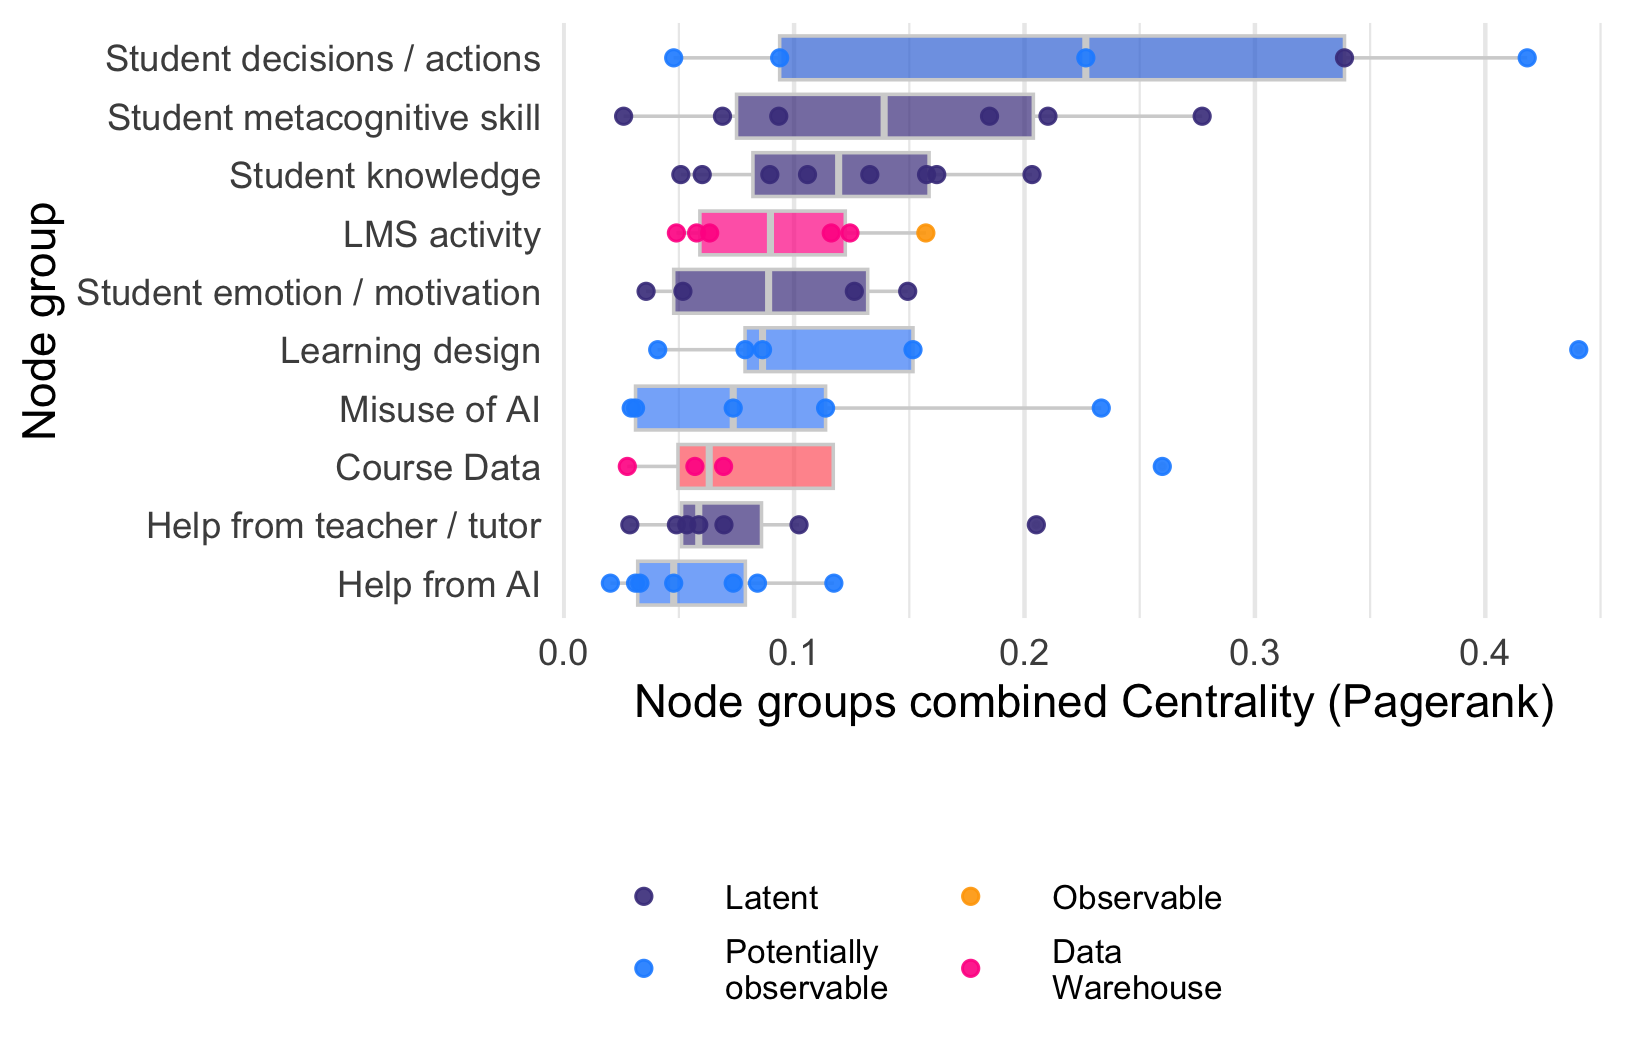
\includegraphics[keepaspectratio]{elicited-DAG-analysis_files/figure-pdf/unnamed-chunk-45-1.png}}

\begin{Shaded}
\begin{Highlighting}[]
\CommentTok{\# }
\CommentTok{\# \# extract legend}
\CommentTok{\# leg \textless{}{-} get\_legend(p\_top\_node\_pagerank\_no\_outcome\_measurability\_discrete)}
\CommentTok{\# }
\CommentTok{\# \# arrange with relative heights (legend gets a small slice)}
\CommentTok{\# p\_node\_importance\_with\_measurability \textless{}{-} (wrap\_elements(leg) /}
\CommentTok{\#     (p\_top\_node\_pagerank\_no\_outcome\_measurability\_discrete + theme(legend.position = "none"))) +}
\CommentTok{\#   plot\_layout(heights = c(0.2, 1))}


\FunctionTok{ggsave}\NormalTok{(}\StringTok{"figures/FIG{-}{-}node\_pagerank\_no\_outcome\_measurability.jpg"}\NormalTok{,}
\NormalTok{       p\_top\_node\_pagerank\_no\_outcome\_measurability\_discrete, }
       \AttributeTok{width =} \DecValTok{5}\NormalTok{, }
       \AttributeTok{height =} \DecValTok{4}\NormalTok{, }
       \AttributeTok{dpi =} \DecValTok{900}\NormalTok{)}
\end{Highlighting}
\end{Shaded}

As table

\begin{Shaded}
\begin{Highlighting}[]
\NormalTok{all\_nodes\_with\_metrics }\SpecialCharTok{|\textgreater{}} 
    \FunctionTok{distinct}\NormalTok{(name, measurability) }\SpecialCharTok{|\textgreater{}} 
\NormalTok{    janitor}\SpecialCharTok{::}\FunctionTok{tabyl}\NormalTok{(measurability) }\SpecialCharTok{|\textgreater{}} 
\NormalTok{    janitor}\SpecialCharTok{::}\FunctionTok{adorn\_totals}\NormalTok{(}\StringTok{"row"}\NormalTok{)}
\end{Highlighting}
\end{Shaded}

\begin{verbatim}
 measurability  n    percent
            DW  5 0.06756757
             O  9 0.12162162
            PO 26 0.35135135
             L 34 0.45945946
         Total 74 1.00000000
\end{verbatim}

\begin{Shaded}
\begin{Highlighting}[]
\CommentTok{\# Pagerank no outcome {-} dist to traced version {-} old}

\NormalTok{d\_ng\_trace\_importance }\OtherTok{\textless{}{-}} 
\NormalTok{    all\_node\_groups\_aggregated\_metrics }\SpecialCharTok{|\textgreater{}} 
    \FunctionTok{inner\_join}\NormalTok{(all\_node\_groups\_distance\_to\_traced, }\AttributeTok{by =} \FunctionTok{c}\NormalTok{(}\StringTok{"Model"}\NormalTok{, }\StringTok{"node\_group"}\NormalTok{)) }\SpecialCharTok{|\textgreater{}} 
    \FunctionTok{filter}\NormalTok{(node\_group }\SpecialCharTok{!=} \StringTok{"Grade.Outcome"}\NormalTok{) }\SpecialCharTok{|\textgreater{}}
    \FunctionTok{inner\_join}\NormalTok{(node\_group\_nice\_name, }\AttributeTok{by =} \StringTok{"node\_group"}\NormalTok{) }\SpecialCharTok{|\textgreater{}}
    \FunctionTok{mutate}\NormalTok{(}\AttributeTok{node\_group =}\NormalTok{ nice\_name) }\SpecialCharTok{|\textgreater{}}
    \FunctionTok{group\_by}\NormalTok{(node\_group) }\SpecialCharTok{|\textgreater{}}
    \FunctionTok{mutate}\NormalTok{(}\AttributeTok{p\_traced\_group =} \FunctionTok{mean}\NormalTok{(m\_dist\_to\_trace)) }\SpecialCharTok{|\textgreater{}}
    \FunctionTok{ungroup}\NormalTok{() }\SpecialCharTok{|\textgreater{}} 
    \FunctionTok{mutate}\NormalTok{(}\AttributeTok{node\_group =} \FunctionTok{fct\_reorder}\NormalTok{(node\_group, pagerank\_no\_outcome)) }\SpecialCharTok{|\textgreater{}} 
    \FunctionTok{arrange}\NormalTok{(}\FunctionTok{desc}\NormalTok{(node\_group)) }\SpecialCharTok{|\textgreater{}} 
    \FunctionTok{filter}\NormalTok{(n }\SpecialCharTok{\textgreater{}} \DecValTok{3}\NormalTok{) }\CommentTok{\# need at least half the models with node group}


\NormalTok{p\_top\_node\_pagerank\_no\_outcome\_trace\_dist }\OtherTok{\textless{}{-}} 
\NormalTok{    d\_ng\_trace\_importance }\SpecialCharTok{|\textgreater{}} 
    \CommentTok{\# arrange(Model, node\_group) |\textgreater{} }
    \FunctionTok{ggplot}\NormalTok{(}\FunctionTok{aes}\NormalTok{(}\AttributeTok{x =}\NormalTok{ pagerank\_no\_outcome, }\AttributeTok{y =}\NormalTok{ node\_group)) }\SpecialCharTok{+}
    \FunctionTok{geom\_boxplot}\NormalTok{(}\FunctionTok{aes}\NormalTok{(}\AttributeTok{fill =}\NormalTok{ p\_traced\_group), }\AttributeTok{colour =} \StringTok{"lightgray"}\NormalTok{, }\AttributeTok{size =} \FloatTok{0.4}\NormalTok{, }\AttributeTok{alpha =} \FloatTok{0.7}\NormalTok{) }\SpecialCharTok{+}
    \CommentTok{\# geom\_line(aes(x = pagerank\_no\_outcome, y = node\_group, group = Model), alpha = 0.6) +}
    \FunctionTok{geom\_point}\NormalTok{(}\FunctionTok{aes}\NormalTok{(}\AttributeTok{colour =}\NormalTok{ m\_dist\_to\_trace), }\AttributeTok{alpha =} \FloatTok{0.9}\NormalTok{) }\SpecialCharTok{+}
    \FunctionTok{scale\_color\_gradient2}\NormalTok{(}
        \AttributeTok{low =} \StringTok{"darkslateblue"}\NormalTok{, }
        \AttributeTok{mid =} \StringTok{"coral"}\NormalTok{,}
        \AttributeTok{high =} \StringTok{"deeppink"}\NormalTok{,}
        \AttributeTok{midpoint =} \FunctionTok{mean}\NormalTok{(}\FunctionTok{range}\NormalTok{(d\_ng\_trace\_importance}\SpecialCharTok{$}\NormalTok{m\_dist\_to\_trace)),}
                         \AttributeTok{breaks =} \FunctionTok{range}\NormalTok{(d\_ng\_trace\_importance}\SpecialCharTok{$}\NormalTok{m\_dist\_to\_trace),}
                         \AttributeTok{labels =} \FunctionTok{c}\NormalTok{(}\StringTok{"Observed"}\NormalTok{,}\StringTok{"Latent"}\NormalTok{),}
                         \AttributeTok{name =} \StringTok{""}\NormalTok{,}
        \AttributeTok{guide =} \FunctionTok{guide\_colorbar}\NormalTok{(}\AttributeTok{reverse =} \ConstantTok{TRUE}\NormalTok{)}
\NormalTok{        ) }\SpecialCharTok{+}
    \FunctionTok{scale\_fill\_gradient2}\NormalTok{(}
        \AttributeTok{midpoint =} \FunctionTok{mean}\NormalTok{(}\FunctionTok{range}\NormalTok{(d\_ng\_trace\_importance}\SpecialCharTok{$}\NormalTok{m\_dist\_to\_trace)),}
        \AttributeTok{low =} \StringTok{"darkslateblue"}\NormalTok{, }
        \AttributeTok{mid =} \StringTok{"coral"}\NormalTok{,}
        \AttributeTok{high =} \StringTok{"deeppink"}
\NormalTok{        ) }\SpecialCharTok{+}
    \FunctionTok{theme\_minimal}\NormalTok{() }\SpecialCharTok{+}
    \FunctionTok{ylab}\NormalTok{(}\StringTok{"Node group"}\NormalTok{) }\SpecialCharTok{+}
    \FunctionTok{xlab}\NormalTok{(}\StringTok{"Node groups combined Centrality (Pagerank)"}\NormalTok{) }\SpecialCharTok{+}
    \CommentTok{\# geom\_rug(aes(colour = m\_dist\_to\_trace), alpha = 0.6, sides = "b") +}
    \CommentTok{\# coord\_cartesian(clip = "off") +}
    \FunctionTok{guides}\NormalTok{(}\AttributeTok{fill =} \StringTok{"none"}\NormalTok{) }\SpecialCharTok{+}
    \FunctionTok{theme}\NormalTok{(}\AttributeTok{legend.position =} \StringTok{"bottom"}\NormalTok{,}
          \AttributeTok{axis.ticks.y =} \FunctionTok{element\_blank}\NormalTok{(),}
          \AttributeTok{axis.line.y =} \FunctionTok{element\_blank}\NormalTok{(),}
          \AttributeTok{panel.grid.major.y =} \FunctionTok{element\_blank}\NormalTok{(),}
          \AttributeTok{panel.grid.minor.y =} \FunctionTok{element\_blank}\NormalTok{())}

\NormalTok{p\_top\_node\_pagerank\_no\_outcome\_trace\_dist}
\end{Highlighting}
\end{Shaded}

\pandocbounded{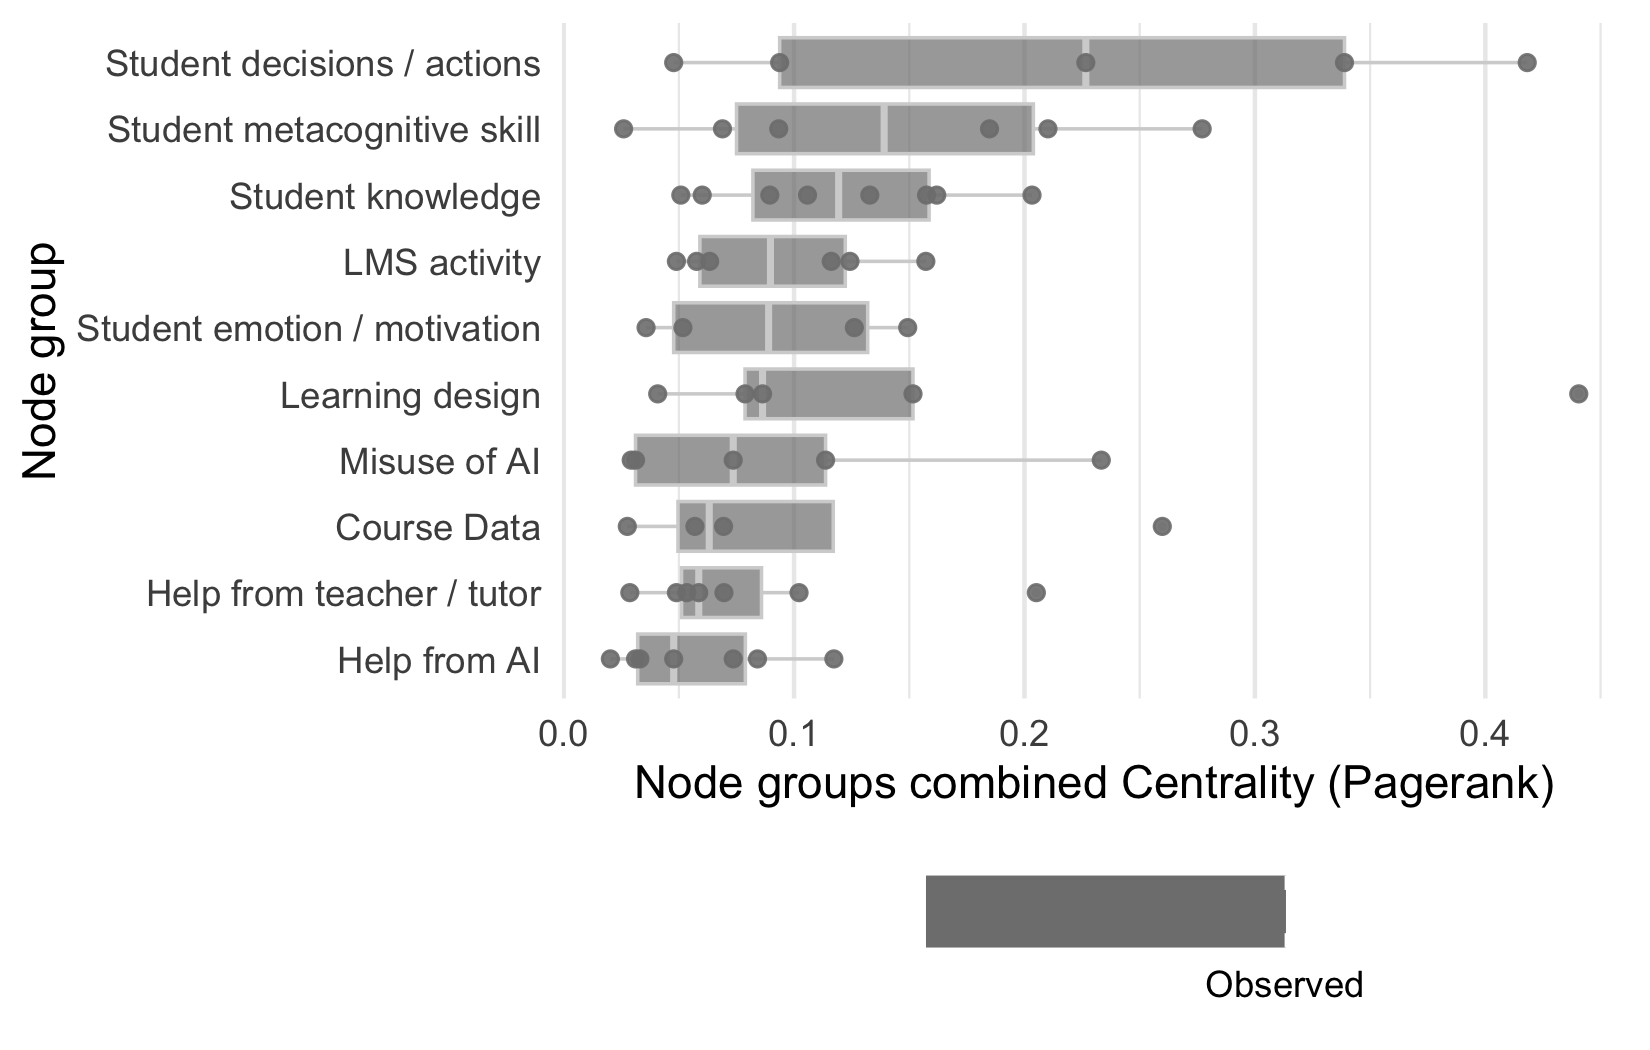
\includegraphics[keepaspectratio]{elicited-DAG-analysis_files/figure-pdf/unnamed-chunk-47-1.png}}

\begin{Shaded}
\begin{Highlighting}[]
\FunctionTok{ggsave}\NormalTok{(}\StringTok{"figures/FIG{-}{-}node\_pagerank\_no\_outcome\_trace\_distance.jpg"}\NormalTok{, p\_top\_node\_pagerank\_no\_outcome\_trace\_dist, }
       \AttributeTok{width =} \DecValTok{5}\NormalTok{, }
       \AttributeTok{height =} \DecValTok{4}\NormalTok{, }
       \AttributeTok{dpi =} \DecValTok{900}\NormalTok{)}

\NormalTok{d\_ng\_trace\_importance }\SpecialCharTok{|\textgreater{}} 
    \FunctionTok{group\_by}\NormalTok{(node\_group) }\SpecialCharTok{|\textgreater{}} 
    \FunctionTok{summarise}\NormalTok{(}\AttributeTok{m\_dist\_to\_trace =} \FunctionTok{mean}\NormalTok{(m\_dist\_to\_trace)) }\SpecialCharTok{|\textgreater{}} 
    \FunctionTok{arrange}\NormalTok{(}\FunctionTok{desc}\NormalTok{(m\_dist\_to\_trace)) }
\end{Highlighting}
\end{Shaded}

\begin{verbatim}
# A tibble: 10 x 2
   node_group                   m_dist_to_trace
   <fct>                                  <dbl>
 1 Course Data                           Inf   
 2 LMS activity                          Inf   
 3 Student emotion / motivation            1.96
 4 Misuse of AI                            1.8 
 5 Help from teacher / tutor               1.79
 6 Learning design                         1.67
 7 Student knowledge                       1.62
 8 Help from AI                            1.57
 9 Student decisions / actions             1.43
10 Student metacognitive skill             1.33
\end{verbatim}

Above plot but lines joining models that are like?

\paragraph{Table: Node lists, with types, groups and importance
metrics}\label{table-node-lists-with-types-groups-and-importance-metrics}

\begin{Shaded}
\begin{Highlighting}[]
\CommentTok{\# could add distance to traced}
\NormalTok{node\_groups\_table }\OtherTok{\textless{}{-}} 
\NormalTok{    all\_nodes\_with\_metrics }\SpecialCharTok{|\textgreater{}}
    \FunctionTok{inner\_join}\NormalTok{(name\_node\_nice\_name, }\AttributeTok{by =} \StringTok{"name"}\NormalTok{) }\SpecialCharTok{|\textgreater{}} 
    \FunctionTok{mutate}\NormalTok{(}\AttributeTok{name =} \FunctionTok{if\_else}\NormalTok{(}
\NormalTok{        node\_group }\SpecialCharTok{==} \StringTok{"H.AI.good"} \SpecialCharTok{\&}\NormalTok{ measurability }\SpecialCharTok{==} \StringTok{"Traced"}\NormalTok{,}
        \FunctionTok{str\_c}\NormalTok{(nice\_name, }\StringTok{"*"}\NormalTok{),}
\NormalTok{        nice\_name}
\NormalTok{    )) }\SpecialCharTok{|\textgreater{}} 
    \FunctionTok{inner\_join}\NormalTok{(node\_group\_nice\_name }\SpecialCharTok{|\textgreater{}} \FunctionTok{rename}\NormalTok{(}\AttributeTok{ng\_nice\_name =}\NormalTok{ nice\_name), }\AttributeTok{by =} \StringTok{"node\_group"}\NormalTok{) }\SpecialCharTok{|\textgreater{}} 
    \FunctionTok{mutate}\NormalTok{(}\AttributeTok{node\_group =}\NormalTok{ ng\_nice\_name) }\SpecialCharTok{|\textgreater{}} 
    \FunctionTok{group\_by}\NormalTok{(node\_type, node\_group) }\SpecialCharTok{|\textgreater{}}
    \FunctionTok{mutate}\NormalTok{(}\AttributeTok{measurability =} \FunctionTok{case\_when}\NormalTok{(}
        \FunctionTok{all}\NormalTok{(measurability }\SpecialCharTok{==} \StringTok{"Traced"}\NormalTok{) }\SpecialCharTok{\textasciitilde{}} \StringTok{"Traced"}\NormalTok{,}
        \FunctionTok{all}\NormalTok{(measurability }\SpecialCharTok{==} \StringTok{"Untraced"}\NormalTok{) }\SpecialCharTok{\textasciitilde{}} \StringTok{"Untraced"}\NormalTok{,}
        \ConstantTok{TRUE} \SpecialCharTok{\textasciitilde{}} \FunctionTok{str\_c}\NormalTok{(}\StringTok{"Some traced* ("}\NormalTok{, }\FunctionTok{sum}\NormalTok{(measurability }\SpecialCharTok{==} \StringTok{"Traced"}\NormalTok{), }\StringTok{" of "}\NormalTok{, }\FunctionTok{n}\NormalTok{(), }\StringTok{")"}\NormalTok{)}
\NormalTok{    )) }\SpecialCharTok{|\textgreater{}} 
    \FunctionTok{group\_by}\NormalTok{(node\_type, node\_group, measurability) }\SpecialCharTok{|\textgreater{}}
    \FunctionTok{summarise}\NormalTok{(}
        \AttributeTok{nodes =} \FunctionTok{str\_c}\NormalTok{(}\FunctionTok{unique}\NormalTok{(name), }\AttributeTok{collapse =} \StringTok{"; "}\NormalTok{),}
        \AttributeTok{n =} \FunctionTok{sum}\NormalTok{(node\_w),}
        \AttributeTok{pagerank =} \FunctionTok{round}\NormalTok{(}\FunctionTok{sum}\NormalTok{(pagerank\_no\_outcome) }\SpecialCharTok{/} \DecValTok{8}\NormalTok{, }\DecValTok{2}\NormalTok{)}
        \CommentTok{\# ,btw = round(sum(btw\_rel), 3)}
\NormalTok{    ) }\SpecialCharTok{|\textgreater{}} 
    \FunctionTok{mutate}\NormalTok{(}\AttributeTok{pagerank =} \FunctionTok{if\_else}\NormalTok{(node\_group }\SpecialCharTok{==} \StringTok{"Grade.Outcome"}\NormalTok{, }\ConstantTok{NA}\NormalTok{, pagerank)) }\SpecialCharTok{|\textgreater{}} 
    \CommentTok{\# mutate(node\_type = case\_when(}
    \CommentTok{\#     node\_type == "L" \textasciitilde{} "Learning Design",}
    \CommentTok{\#     node\_type == "S" \textasciitilde{} "Student",}
    \CommentTok{\#     node\_type == "T" \textasciitilde{} "Teacher",}
    \CommentTok{\#     node\_type == "C" \textasciitilde{} "Course Data",}
    \CommentTok{\#     node\_type == "G" \textasciitilde{} "Grade Data",}
    \CommentTok{\#     node\_type == "H" \textasciitilde{} "Help"}
    \CommentTok{\# )) |\textgreater{} }
    \FunctionTok{arrange}\NormalTok{(}\FunctionTok{desc}\NormalTok{(n), }\FunctionTok{desc}\NormalTok{(pagerank)) }\SpecialCharTok{|\textgreater{}} 
    \FunctionTok{select}\NormalTok{(node\_group, node\_type, nodes, n, measurability, pagerank) }\SpecialCharTok{|\textgreater{}} 
    \FunctionTok{ungroup}\NormalTok{()}
\end{Highlighting}
\end{Shaded}

\begin{verbatim}
`summarise()` has grouped output by 'node_type', 'node_group'. You can override
using the `.groups` argument.
\end{verbatim}

\begin{Shaded}
\begin{Highlighting}[]
\NormalTok{node\_groups\_table}
\end{Highlighting}
\end{Shaded}

\begin{verbatim}
# A tibble: 21 x 6
   node_group                   node_type     nodes     n measurability pagerank
   <chr>                        <fct>         <chr> <dbl> <chr>            <dbl>
 1 Learning design              Learning des~ Task~    11 Some traced*~     0.1 
 2 Help from AI                 Help          Help~    11 Some traced*~     0.05
 3 Student decisions / actions  Student       Stud~    10 Some traced*~     0.14
 4 Student knowledge            Student       Stud~    10 Some traced*~     0.12
 5 Student metacognitive skill  Student       Stud~     9 Some traced*~     0.11
 6 Help from teacher / tutor    Help          Help~     9 Some traced*~     0.07
 7 Student emotion / motivation Student       Stud~     9 Some traced*~     0.05
 8 LMS activity                 Learning data LMS ~     8 Some traced*~     0.07
 9 Assessment grade             Assessment d~ Asse~     8 Some traced*~     0   
10 Preliminary assessments      Assessment d~ Mark~     7 Some traced*~     0.08
# i 11 more rows
\end{verbatim}

\begin{Shaded}
\begin{Highlighting}[]
\NormalTok{all\_nodes\_with\_metrics }\SpecialCharTok{|\textgreater{}} 
    \FunctionTok{distinct}\NormalTok{(name) }\SpecialCharTok{|\textgreater{}} 
    \FunctionTok{nrow}\NormalTok{() }\SpecialCharTok{|\textgreater{}} 
    \FunctionTok{paste}\NormalTok{(}\StringTok{"distinct nodes"}\NormalTok{)}
\end{Highlighting}
\end{Shaded}

\begin{verbatim}
[1] "74 distinct nodes"
\end{verbatim}

\begin{Shaded}
\begin{Highlighting}[]
\NormalTok{all\_nodes\_with\_metrics }\SpecialCharTok{|\textgreater{}} 
    \FunctionTok{distinct}\NormalTok{(node\_group) }\SpecialCharTok{|\textgreater{}} 
    \FunctionTok{nrow}\NormalTok{() }\SpecialCharTok{|\textgreater{}} 
    \FunctionTok{paste}\NormalTok{(}\StringTok{"node groups"}\NormalTok{)}
\end{Highlighting}
\end{Shaded}

\begin{verbatim}
[1] "21 node groups"
\end{verbatim}

\begin{Shaded}
\begin{Highlighting}[]
\NormalTok{all\_nodes\_with\_metrics }\SpecialCharTok{|\textgreater{}} 
    \FunctionTok{distinct}\NormalTok{(name, measurability) }\SpecialCharTok{|\textgreater{}} \FunctionTok{count}\NormalTok{(measurability)}
\end{Highlighting}
\end{Shaded}

\begin{verbatim}
# A tibble: 4 x 2
  measurability     n
  <fct>         <int>
1 DW                5
2 O                 9
3 PO               26
4 L                34
\end{verbatim}

\begin{Shaded}
\begin{Highlighting}[]
\NormalTok{tb1 }\OtherTok{\textless{}{-}}\NormalTok{ node\_groups\_table }\SpecialCharTok{|\textgreater{}} \FunctionTok{filter}\NormalTok{(n }\SpecialCharTok{\textgreater{}=} \DecValTok{7}\NormalTok{) }\SpecialCharTok{|\textgreater{}} \FunctionTok{arrange}\NormalTok{(}\FunctionTok{desc}\NormalTok{(n))}
\NormalTok{tb2 }\OtherTok{\textless{}{-}}\NormalTok{ node\_groups\_table }\SpecialCharTok{|\textgreater{}} \FunctionTok{filter}\NormalTok{(n }\SpecialCharTok{\textless{}} \DecValTok{7}\NormalTok{) }\SpecialCharTok{|\textgreater{}} \FunctionTok{arrange}\NormalTok{(}\FunctionTok{desc}\NormalTok{(n))}
\NormalTok{tb1 }\SpecialCharTok{|\textgreater{}}\NormalTok{ clipr}\SpecialCharTok{::}\FunctionTok{write\_clip}\NormalTok{()}
\NormalTok{tb2 }\SpecialCharTok{|\textgreater{}}\NormalTok{ clipr}\SpecialCharTok{::}\FunctionTok{write\_clip}\NormalTok{()}
\end{Highlighting}
\end{Shaded}

What about grouping by the node category first, so it's hierarchical?

\begin{Shaded}
\begin{Highlighting}[]
\NormalTok{node\_types\_table }\OtherTok{\textless{}{-}} 
\NormalTok{    node\_groups\_table }\SpecialCharTok{|\textgreater{}} 
    \FunctionTok{group\_by}\NormalTok{(node\_type) }\SpecialCharTok{|\textgreater{}} 
    \FunctionTok{mutate}\NormalTok{(}\AttributeTok{nt =} \FunctionTok{sum}\NormalTok{(n)) }\SpecialCharTok{|\textgreater{}} 
    \FunctionTok{ungroup}\NormalTok{() }\SpecialCharTok{|\textgreater{}} 
    \FunctionTok{arrange}\NormalTok{(}\FunctionTok{desc}\NormalTok{(nt), }\FunctionTok{desc}\NormalTok{(n)) }\SpecialCharTok{|\textgreater{}} 
    \FunctionTok{select}\NormalTok{(node\_type, nt, node\_group, nodes, n, measurability, pagerank) }\SpecialCharTok{|\textgreater{}} 
    \FunctionTok{mutate}\NormalTok{(}\AttributeTok{node\_type =} \FunctionTok{str\_c}\NormalTok{(node\_type, }\StringTok{" ("}\NormalTok{, nt, }\StringTok{")"}\NormalTok{)) }\SpecialCharTok{|\textgreater{}} 
    \FunctionTok{select}\NormalTok{(}\SpecialCharTok{{-}}\NormalTok{nt)}

\NormalTok{node\_types\_table}
\end{Highlighting}
\end{Shaded}

\begin{verbatim}
# A tibble: 21 x 6
   node_type    node_group                   nodes      n measurability pagerank
   <chr>        <chr>                        <chr>  <dbl> <chr>            <dbl>
 1 Student (44) Student decisions / actions  Stude~    10 Some traced*~     0.14
 2 Student (44) Student knowledge            Stude~    10 Some traced*~     0.12
 3 Student (44) Student metacognitive skill  Stude~     9 Some traced*~     0.11
 4 Student (44) Student emotion / motivation Stude~     9 Some traced*~     0.05
 5 Student (44) Student attributes           Stude~     4 Some traced*~     0.02
 6 Student (44) Student prior knowledge      Stude~     2 Some traced*~     0.01
 7 Help (30)    Help from AI                 Help ~    11 Some traced*~     0.05
 8 Help (30)    Help from teacher / tutor    Help ~     9 Some traced*~     0.07
 9 Help (30)    Misuse of AI                 Misus~     6 Some traced*~     0.06
10 Help (30)    Help from peers              Help ~     3 Some traced*~     0.01
# i 11 more rows
\end{verbatim}

\begin{Shaded}
\begin{Highlighting}[]
\NormalTok{tbt1 }\OtherTok{\textless{}{-}}\NormalTok{ node\_types\_table }\SpecialCharTok{|\textgreater{}} \FunctionTok{filter}\NormalTok{(}\FunctionTok{str\_detect}\NormalTok{(node\_type, }\StringTok{"Student|Help"}\NormalTok{))}
\NormalTok{tbt2 }\OtherTok{\textless{}{-}}\NormalTok{ node\_types\_table }\SpecialCharTok{|\textgreater{}} \FunctionTok{filter}\NormalTok{(}\SpecialCharTok{!}\FunctionTok{str\_detect}\NormalTok{(node\_type, }\StringTok{"Student|Help"}\NormalTok{))}
\NormalTok{tbt1 }\SpecialCharTok{|\textgreater{}}\NormalTok{ clipr}\SpecialCharTok{::}\FunctionTok{write\_clip}\NormalTok{()}
\NormalTok{tbt2 }\SpecialCharTok{|\textgreater{}}\NormalTok{ clipr}\SpecialCharTok{::}\FunctionTok{write\_clip}\NormalTok{()}
\end{Highlighting}
\end{Shaded}

\subsection{Edge / path importance}\label{edge-path-importance}

\begin{Shaded}
\begin{Highlighting}[]
\NormalTok{all\_edge\_group\_with\_metrics }\OtherTok{\textless{}{-}}
\NormalTok{    edges\_with\_metrics }\SpecialCharTok{|\textgreater{}} 
    \FunctionTok{mutate}\NormalTok{(}\AttributeTok{from =} \FunctionTok{code\_node\_group}\NormalTok{(from),}
           \AttributeTok{to =} \FunctionTok{code\_node\_group}\NormalTok{(to)) }\SpecialCharTok{|\textgreater{}} 
    \FunctionTok{group\_by}\NormalTok{(from, to) }\SpecialCharTok{|\textgreater{}} 
    \FunctionTok{summarise}\NormalTok{(}
        \AttributeTok{n =} \FunctionTok{sum}\NormalTok{(n),}
        \AttributeTok{max\_n =} \FunctionTok{sum}\NormalTok{(max\_n),}
        \AttributeTok{edge\_p\_w =} \FunctionTok{mean}\NormalTok{(edge\_p\_w),}
        \AttributeTok{p\_aligned =} \FunctionTok{mean}\NormalTok{(switched }\SpecialCharTok{==} \StringTok{"aligned"}\NormalTok{)}
\NormalTok{    )}
\end{Highlighting}
\end{Shaded}

\begin{verbatim}
`summarise()` has grouped output by 'from'. You can override using the
`.groups` argument.
\end{verbatim}

\begin{Shaded}
\begin{Highlighting}[]
\NormalTok{edge\_group\_analysis\_edgelist }\OtherTok{\textless{}{-}}\NormalTok{ all\_edge\_group\_with\_metrics }\SpecialCharTok{|\textgreater{}} 
    \FunctionTok{mutate}\NormalTok{(}\AttributeTok{edge\_w =}\NormalTok{ n }\SpecialCharTok{+}\NormalTok{ edge\_p\_w }\SpecialCharTok{*}\NormalTok{ n) }\SpecialCharTok{|\textgreater{}} 
    \FunctionTok{arrange}\NormalTok{(}\FunctionTok{desc}\NormalTok{(edge\_w))}


\CommentTok{\# the node group one here isn\textquotesingle{}t one row per node group, and doesn\textquotesingle{}t have the node type!}
\NormalTok{edge\_group\_analysis\_graph }\OtherTok{\textless{}{-}} \FunctionTok{tbl\_graph}\NormalTok{(}
    \AttributeTok{nodes =}\NormalTok{ all\_node\_groups\_aggregated\_metrics }\SpecialCharTok{|\textgreater{}} 
        \FunctionTok{rename}\NormalTok{(}\AttributeTok{name =}\NormalTok{ node\_group) }\SpecialCharTok{|\textgreater{}} 
        \FunctionTok{group\_by}\NormalTok{(name, node\_type) }\SpecialCharTok{|\textgreater{}} 
        \FunctionTok{summarise}\NormalTok{(}
            \AttributeTok{p\_traced =} \FunctionTok{mean}\NormalTok{(p\_traced),}
            \AttributeTok{pgrnk =} \FunctionTok{mean}\NormalTok{(pagerank\_no\_outcome),}
            \AttributeTok{node\_w =} \FunctionTok{sum}\NormalTok{(n)}
\NormalTok{        ) , }
    \AttributeTok{edges =}\NormalTok{ edge\_group\_analysis\_edgelist)}
\end{Highlighting}
\end{Shaded}

\begin{verbatim}
`summarise()` has grouped output by 'name'. You can override using the
`.groups` argument.
\end{verbatim}

\begin{Shaded}
\begin{Highlighting}[]
\NormalTok{edge\_group\_analysis\_graph }\SpecialCharTok{\%N\textgreater{}\%}
    \FunctionTok{arrange}\NormalTok{(name) }\SpecialCharTok{|\textgreater{}} 
    \CommentTok{\# activate(edges) |\textgreater{}}
    \CommentTok{\# filter(edge\_w \textgreater{} 8) |\textgreater{}}
    \FunctionTok{ggraph}\NormalTok{(}
        \AttributeTok{layout =} \StringTok{"circle"}
        \CommentTok{\# layout = "sugiyama"}
\NormalTok{        ) }\SpecialCharTok{+}
            \FunctionTok{geom\_edge\_diagonal}\NormalTok{(}
                \FunctionTok{aes}\NormalTok{(}\AttributeTok{alpha =}\NormalTok{ edge\_w), }
                          \AttributeTok{strength =} \FloatTok{0.5}\NormalTok{,}
                          \AttributeTok{arrow =} \FunctionTok{arrow}\NormalTok{(}\AttributeTok{length =} \FunctionTok{unit}\NormalTok{(}\DecValTok{3}\NormalTok{, }\StringTok{\textquotesingle{}mm\textquotesingle{}}\NormalTok{),}
                                        \AttributeTok{type =} \StringTok{"closed"}\NormalTok{),}
                          \AttributeTok{start\_cap =} \FunctionTok{circle}\NormalTok{(}\DecValTok{2}\NormalTok{, }\StringTok{\textquotesingle{}mm\textquotesingle{}}\NormalTok{),}
                          \AttributeTok{end\_cap =} \FunctionTok{circle}\NormalTok{(}\DecValTok{3}\NormalTok{, }\StringTok{\textquotesingle{}mm\textquotesingle{}}\NormalTok{)) }\SpecialCharTok{+}
    \FunctionTok{geom\_node\_point}\NormalTok{(}\FunctionTok{aes}\NormalTok{(}\AttributeTok{size =}\NormalTok{ pgrnk, }\AttributeTok{color =}\NormalTok{ node\_type)) }\SpecialCharTok{+}
    \FunctionTok{geom\_node\_text}\NormalTok{(}\FunctionTok{aes}\NormalTok{(}\AttributeTok{label =}\NormalTok{ name), }\AttributeTok{repel =} \ConstantTok{TRUE}\NormalTok{) }\SpecialCharTok{+}
    \FunctionTok{scale\_edge\_alpha}\NormalTok{(}\AttributeTok{range =} \FunctionTok{c}\NormalTok{(}\FloatTok{0.1}\NormalTok{,}\DecValTok{9}\NormalTok{)) }\SpecialCharTok{+}
    \FunctionTok{theme\_graph}\NormalTok{()}
\end{Highlighting}
\end{Shaded}

\pandocbounded{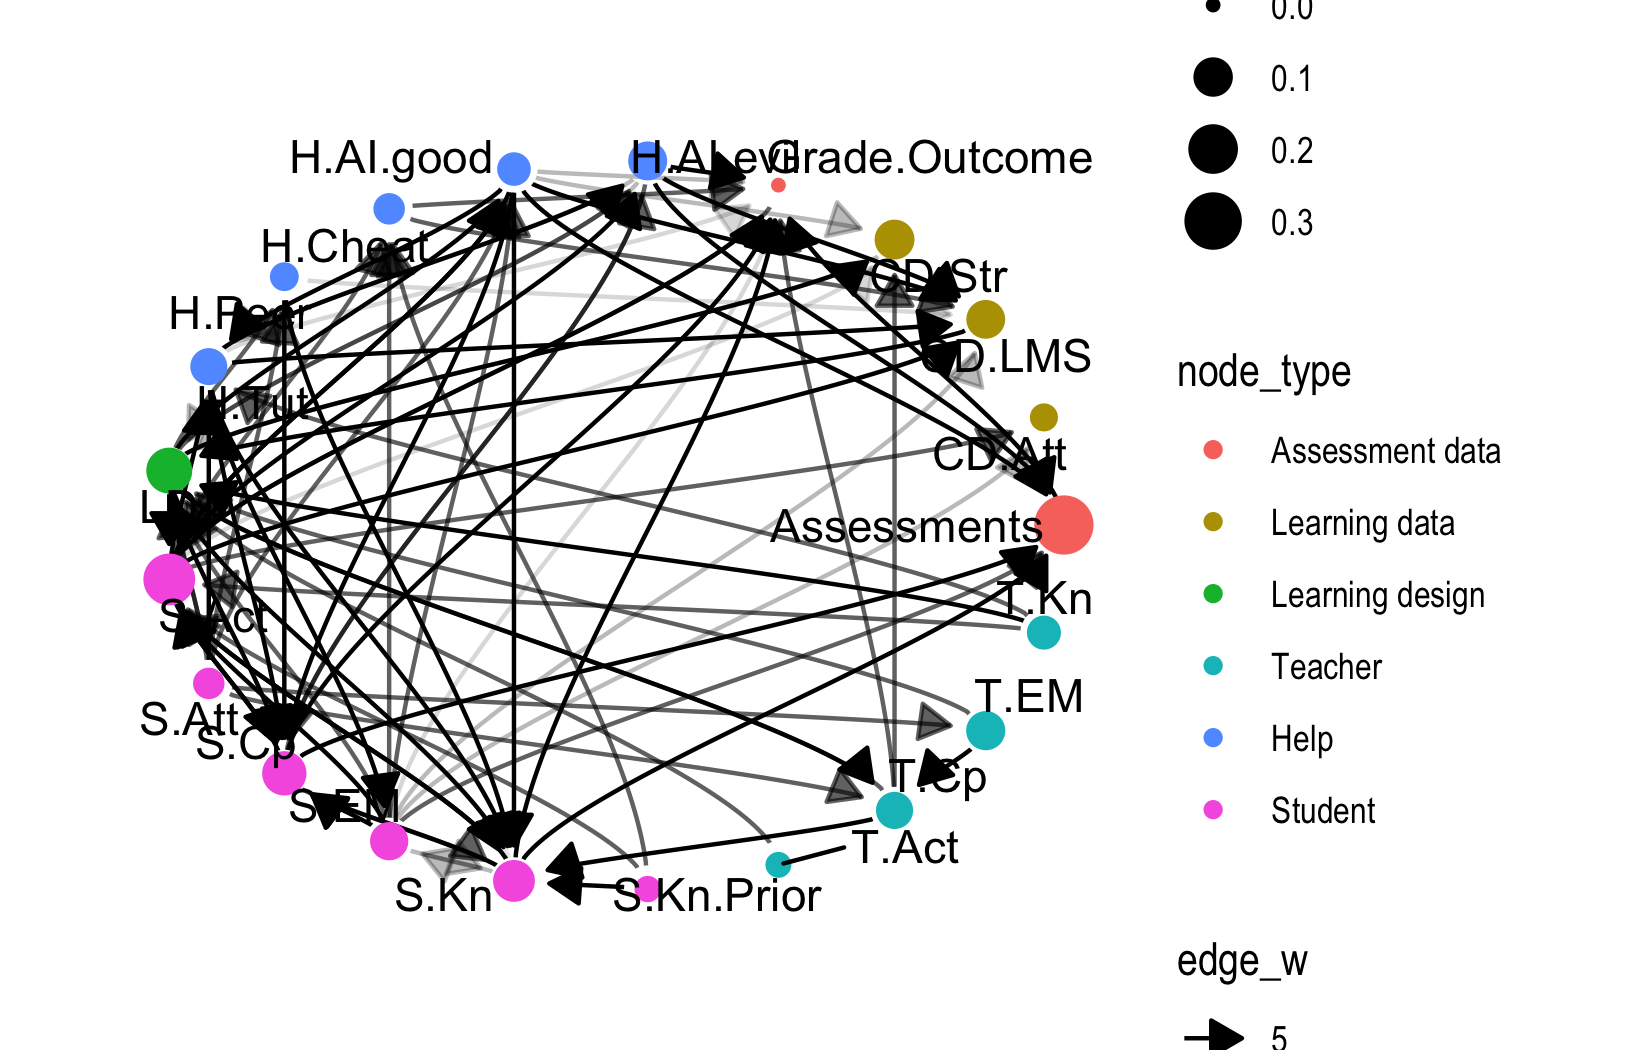
\includegraphics[keepaspectratio]{elicited-DAG-analysis_files/figure-pdf/unnamed-chunk-52-1.png}}

Path importance - what about the sets of implied conditional
independencies? Is there a way to look at the sets of these and see if
any contradict each other??




\end{document}
